\documentclass[12pt, a4paper]{book}
\usepackage[utf8]{inputenc}
\usepackage[T1]{fontenc}
\usepackage[default, scale=.95]{opensans} % police Open Sans
\usepackage{setspace}
\usepackage{amsmath}
\newcommand\numberthis{\addtocounter{equation}{1}\tag{\theequation}}
\usepackage{amsfonts}
\usepackage{fancyhdr}
\usepackage{amssymb}
\usepackage[nottoc, notlof, notlot]{tocbibind}
\usepackage{xcolor} % ou color selon l'installation
\definecolor{Prune}{RGB}{99,0,60} % l14-33 : couleurs de la charte graphique upsaclay
\definecolor{B1}{RGB}{49,62,72}
\definecolor{C1}{RGB}{124,135,143}
\definecolor{D1}{RGB}{213,218,223}
\definecolor{A2}{RGB}{198,11,70}
\definecolor{B2}{RGB}{237,20,91}
\definecolor{C2}{RGB}{238,52,35}
\definecolor{D2}{RGB}{243,115,32}
\definecolor{A3}{RGB}{124,42,144}
\definecolor{B3}{RGB}{125,106,175}
\definecolor{C3}{RGB}{198,103,29}
\definecolor{D3}{RGB}{254,188,24}
\definecolor{A4}{RGB}{0,78,125}
\definecolor{B4}{RGB}{14,135,201}
\definecolor{C4}{RGB}{0,148,181}
\definecolor{D4}{RGB}{70,195,210}
\definecolor{A5}{RGB}{0,128,122}
\definecolor{B5}{RGB}{64,183,105}
\definecolor{C5}{RGB}{140,198,62}
\definecolor{D5}{RGB}{213,223,61}
\usepackage{mdframed}
\usepackage{multirow} %% Pour mettre un texte sur plusieurs rangées
\usepackage{multicol} %% Pour mettre un texte sur plusieurs colonnes
\usepackage{scrextend} %Forcer la 4ème  de couverture en page pair
\usepackage{tikz}
\usepackage{graphicx}
\usepackage[absolute]{textpos}
\usepackage{colortbl}
\usepackage{float}
\usepackage{array}
\usepackage{geometry}
\usepackage{titlesec}
\usepackage[strict]{changepage}
\usepackage{acronym}   	 	% list of abbreviations / acronyms

% Drawing with tikz
\usepackage{tikz}
\usetikzlibrary{shapes.geometric, arrows, positioning}

% Caption setup
\usepackage{caption}
\captionsetup{labelfont=bf}
\captionsetup[figure]{font={stretch=1.5}}
\captionsetup[table]{font={stretch=1.5}}
% paramétrage couleur des liens hypertextes, toujours garder colorlinks=true
\usepackage{hyperref}
\hypersetup{
    colorlinks=true,
    linkcolor=black,
    urlcolor=purple,
    citecolor=purple
}
\usepackage[capitalise, noabbrev]{cleveref}

\pagestyle{plain} % pour ne garder que les n°de page en milieu-bas et supprimer les indications de chapitre en marge haute

% Code blocks formatting
\usepackage{listings}

\definecolor{dkgreen}{rgb}{0,0.6,0}
\definecolor{gray}{rgb}{0.5,0.5,0.5}
\definecolor{mauve}{rgb}{0.58,0,0.82}

\lstset{
  frame=tb,
  showstringspaces=false,
  columns=flexible,
  basicstyle={\small\ttfamily},
  numbers=left,
  numberstyle=\tiny\color{gray},
  numbersep=5pt,
  keywordstyle=\color{blue},
  commentstyle=\color{dkgreen},
  stringstyle=\color{mauve},
  breaklines=true,
  breakatwhitespace=true,
  tabsize=4
}

% Maths macros
% % --- Our (additional) packages --- %
%  \usepackage{color}
%  \usepackage{makeidx}
\usepackage{here}
% \usepackage{algorithm,algorithmic}
\usepackage{algorithm}

 \usepackage{faktor}
 \usepackage{xspace}
 \usepackage{amsfonts,amsthm,amsmath,amssymb}
 \usepackage[T1]{fontenc}
 \usepackage{graphicx}
 \usepackage{subcaption}
 \usepackage{pstricks}
%

\newtheorem{theorem}{Theorem}
\newtheorem{lemma}{Lemma}
\newtheorem{proposition}{Proposition}
\newtheorem{remark}{Remark}
\newtheorem{definition}{Definition}
\newtheorem{conjecture}{Conjecture}
\newtheorem{corollary}{Corollary}

% ---Algos --- %

%\SetKwInput{KwInput}{Input}
%\SetKwInput{KwInit}{Initialization}
% \usepackage{algorithm2e}
\newtheorem*{conjecture*}{Conjecture}
% --- Commands --- %
\DeclareMathOperator*{\argmax}{arg\,max}
\DeclareMathOperator*{\argmin}{arg\,min}

\newcommand{\id}{\mathrm{id}}
\newcommand{\MAP}{\mathrm{MAP}}
\newcommand{\eps}{\varepsilon}
\newcommand{\ind}{\mathbf{1}_}
\newcommand{\R}{{\mathbb{R}}}
\newcommand{\C}{{\mathbb{C}}}
\newcommand{\Var}{{\mathrm{Var}}}
\newcommand{\tr}{{\rm tr}}
\newcommand{\Tr}{{\rm Tr}}
\newcommand{\dT}{\mathbb {T}}
\newcommand{\dE}{\mathbb {E}}
\newcommand{\dL}{\mathbb {L}}
\newcommand{\dP}{\mathbb{P}}
\newcommand{\dQ}{\mathbb{Q}}
\newcommand{\dN}{\mathbb {N}}
\newcommand{\dR}{\mathbb {R}}
\newcommand{\dC}{\mathbb {C}}
\newcommand{\dG}{\mathbb {G}}
\newcommand{\cF}{\mathcal {F}}
\newcommand{\dH}{\mathbb{H}}
\newcommand{\cE}{\mathcal {E}}
\newcommand{\cO}{\mathcal {O}}
\newcommand{\cA}{\mathcal {A}}
\newcommand{\cB}{\mathcal {B}}
\newcommand{\cG}{\mathcal {G}}
\newcommand{\cH}{\mathcal {H}}
\newcommand{\cX}{\mathcal {X}}
\newcommand{\cL}{\mathcal {L}}
\newcommand{\cK}{\mathcal {K}}
\newcommand{\cW}{\mathcal {W}}
\newcommand{\cP}{\mathcal {P}}
\newcommand{\cV}{\mathcal {V}}
\newcommand{\cC}{\mathcal {C}}
\newcommand{\cI}{\mathcal {I}}
\newcommand{\cN}{\mathcal {N}}
\newcommand{\cM}{\mathcal {M}}
\newcommand{\cS}{\mathcal {S}}
\newcommand{\cD}{\mathcal {D}}
\newcommand{\cT}{\mathcal {T}}
\newcommand{\cY}{\mathcal {Y}}
\newcommand{\cZ}{\mathcal {Z}}
\newcommand{\cQ}{\mathcal {Q}}
\newcommand{\cR}{\mathcal {R}}

\newcommand{\fm}{\mathfrak{m}}


\newcommand{\Bin}{ \mathrm{Bin}}
\newcommand{\GW}{ \mathrm{GW}}
\newcommand{\Poi}{ \mathrm{Poi}}
\newcommand{\Ber}{\mathrm{Ber}}
\newcommand{\DTV}{{\mathrm{d_{TV}}}}
\newcommand{\ov}{{\mathrm{ov}}}
\newcommand{\Ent}{\mathrm{Ent}}
\newcommand{\KL}{\mathrm{KL}}
\newcommand{\loss}{\mathrm{loss}}

\newcommand{\err}{\mathrm{err}}

\newcommand{\bt}{\mathbf{t}}
\newcommand{\btau}{\boldsymbol{\tau}}
\newcommand{\bsigma}{\boldsymbol{\mathsf{\sigma}}}
\newcommand{\bd}{\mathbf{d}}
\newcommand{\bL}{\mathbf{L}}
\newcommand{\br}{\mathbf{r}}
\newcommand{\bA}{\mathbf{A}}
\newcommand{\bDelta}{\boldsymbol{\Delta}}
\newcommand{\Aut}{\mathrm{Aut}}
\newcommand{\bX}{\mathbf{X}}
\newcommand{\bU}{\mathbf{U}}
\newcommand{\bD}{\mathbf{D}}
\newcommand{\bC}{\mathbf{C}}
\newcommand{\bM}{\mathbf{M}}
\newcommand{\bV}{\mathbf{V}}
\newcommand{\bN}{\mathbf{N}}
\newcommand{\bZ}{\mathbf{Z}}
\newcommand{\bw}{\mathbf{w}}
\newcommand{\bK}{\mathbf{K}}
\newcommand{\bY}{\mathbf{Y}}
\newcommand{\bG}{\mathbf{G}}
\newcommand{\bcM}{\boldsymbol{\cM}}


\newcommand{\vol}{V}
\newcommand{\sign}{ \mathrm{sign}}
\newcommand{\diag}{ \mathrm{diag}}
\newcommand{\supp}{ \mathrm{supp}}
\newcommand{\var}{\hbox{Var}}
\newcommand{\cov}{\hbox{Cov}}
\newcommand{\ER}{Erd\H{o}s-R\'enyi }

\newcommand{\card}[1]{\left|{#1} \right|}
\newcommand{\poly}{\mathrm{poly}}
\newcommand{\bT}{\mathbf{T}}
\newcommand{\btheta}{\boldsymbol{\theta}}
\newcommand{\bc}{\mathbf{c}}
% \newcommand{\bV}{\mathbf{V}}

\newcommand{\pext}{p_{\mathrm{ext}}}

\newcommand{\inj}{\hookrightarrow}

\newcommand{\ts}{\textsuperscript}

\newcommand{\luca}[1]{({\color{purple} LG: #1})}


\begin{document}

\begin{titlepage}

  %\thispagestyle{empty}

  \newgeometry{left=6cm,bottom=2cm, top=1cm, right=1cm}

  \tikz[remember picture,overlay] \node[opacity=1,inner sep=0pt] at (-13mm,-135mm){
\includegraphics{images/Frame-ups.pdf}};

  %*****************************************************
  %******** NUMÉRO D'ORDRE DE LA THÈSE À COMPLÉTER *****
  %******** POUR LE SECOND DÉPOT                   *****
  %*****************************************************

  \color{white}

  \begin{picture}(0,0)
    \put(-152,-743){\rotatebox{90}{\Large \textsc{THESE DE DOCTORAT}}} \\
    \put(-120,-743){\rotatebox{90}{NNT : 2020UPASA001}}
  \end{picture}

  %*****************************************************
  %******************** TITRE **************************
  %*****************************************************

  \flushright
  \vspace{10mm} % à régler éventuellement
  \color{Prune}
  \fontfamily{cmss}\fontseries{m}\fontsize{22}{26}\selectfont
  \Huge Geographic and socio-demographic disparities in oncology care pathways \\

  \normalsize
  \color{black}
  \Large{\textit{
      Etude des disparités géographiques et socio-démographiques dans les parcours de soins en oncologie
    }} \\
  %*****************************************************

  \fontfamily{fvs}\fontseries{m}\fontsize{8}{12}\selectfont

  \vspace{1.5cm}

  \normalsize
  \textbf{Thèse de doctorat de l'université Paris-Saclay} \\

  \vspace{6mm}

  \small École doctorale n$^{\circ}$ 582, Cancérologie : Biologie, Médecine et Santé (CBMS)\\
  \small Spécialité de doctorat: Recherche clinique, innovation technologique, santé publique \\
  \vspace{6mm}

  \footnotesize Thèse préparée dans les unités de recherche de l'Institut Curie et INRIA, sous la direction de Fabien Reyal, MD, PhD, et la co-direction de Marc Lelarge, PhD.\\
  \vspace{15mm}

  \textbf{Thèse soutenue à Paris-Saclay, le 12 Décembre 2022, par}\\
  \bigskip
  \Large {\color{Prune} \textbf{Eric DAOUD-ATTOYAN}} %

  %************************************
  \vspace{\fill} % ALIGNER LE TABLEAU EN BAS DE PAGE
  %************************************

  \bigskip

  \flushleft
  \small \textbf{Composition du jury}\\
  \vspace{2mm}
  \scriptsize
  \begin{tabular}{|p{7cm}l}
    \arrayrulecolor{Prune}

    \textbf{François Alla}                     & Examinateur                \\
    Université de Bordeaux                     &                            \\
    \textbf{Stéphanie Allassonnière}           & Examinatrice               \\
    Univeristé Paris-Cité                      &                            \\
    \textbf{Gaël Varoquaux}                    & Examinateur                \\
    Université Paris-Saclay                    &                            \\
    \textbf{Inès Vaz-Duarte-Luis}              & Examinatrice               \\
    Université Paris-Saclay                    &                            \\
    \textbf{Gwenn Menvielle}                   & Rapporteur \& Examinatrice \\
    Inserm, Sorbonne Université, Paris, France &                            \\
    \textbf{Raphaël Porcher}                   & Rapporteur \& Examinateur  \\
    Université Paris-Cité                      &                            \\
    \textbf{Marc Lelarge}                      & Co-Directeur de thèse      \\
    INRIA, DI/ENS, PSL Research University     &                            \\
    \textbf{Fabien Reyal}                      & Directeur de thèse         \\
    Institut Curie, Université Paris-Cité      &                            \\
  \end{tabular}

\end{titlepage}

%***************************
%***** Acknowledgement *****
%***************************

\newgeometry{top=4cm, bottom=4cm, left=2cm, right=2cm}

\begin{singlespace}
  \setstretch{1.5}
  \chapter*{Acknowledgements}

% Jury & rapporteurs
Je remercie tout d'abord les membres du jury pour avoir accepté de suivre mon
travail: Pr. François Alla, Pr. Stéphanie Allassonnière, Gaël Varoquaux et Inès
Vaz-Duarte-Luis. Un grand merci également à mes deux rapporteurs, Pr. Raphaël
Porcher et Gwenn Menvielle pour avoir pris le temps de relire mon manuscrit. Je
suis honoré d'être encadré par ces grands médecins et chercheurs que je n'aurais
jamais imaginé rencontrer.

% Superviseurs
Ensuite, un immense merci à mes deux superviseurs de thèse, Pr. Fabien Reyal et
Marc Lelarge, pour m'avoir fait confiance dès le début et pour votre encadrement
de qualité pendant ces trois ans. J'ai beaucoup appris grâce à vous et j'en
ressors grandi. Merci Fabien pour tes innombrables intuitions, ta franchise et
ton exigence, particulièrement sur la visualisation de données. Tu as su faire
le pont entre la médecine et la recherche en informatique, qui m'a permis de
garder en tête le besoin des patients tout au long de mes projets. Merci Marc
pour ton calme, ta rigueur, ta pédagogie et ton immense expertise en Machine
Learning notamment. Tu as accepté de me superviser en cours de thèse et je t'en
suis très reconnaissant, ma thèse n'aurait pas été la même sans ton aide.

% Research teams
J'ai eu la chance de travailler dans deux équipes de recherche, le RT2 Lab de
l'Institut Curie et l'équipe Dyogene de l'INRIA Paris. Mes premiers
remerciements vont au RT2Lab. Tout d'abord merci à Elise et Beatriz, mes
co-thésardes avec qui nous avons résolu bien des problèmes autant scientifiques
qu'administratifs, et qui m'ont permis de garder le sourire pendant toute ma
thèse. Ensuite, Judith sans qui je n'aurais jamais commencé cette thèse et qui
m'a été d'excellent conseil tout au long de mon parcours. Merci à Anne-Sophie,
pour son accompagnement, ses conseils et son expertise dans la recherche
médicale. Merci à Nadir, Lidia, Amyn, Dorian, Jeanne, Aullène, Marie, Zoé,
Emile, Jade, Eva, Sara et Imane pour avoir apporté une nouvelle dynamique à
l'équipe. Enfin merci à Floriane, Paul nouveaux thésards de l'équipe, pour leurs
conseils et leur aide, je vous souhaite le meilleur. Un grand merci également à
Dominique, sans qui je n'aurais jamais pu survivre administrativement à
l'Institut Curie. Ensuite, mes remerciements vont à l'équipe Dyogene. Je
remercie d'abord mes collègues de bureau, dit ``le bureau des boloss''. Luca, tu
es la première personne que j'ai croisé à l'INRIA et je te remercie infiniment
pour ton accueil, pour m'avoir intégré dans l'équipe, mais aussi pour nos
footings et sessions musique. Matthieu, Mathieu et Bastien, je vous remercie
pour votre bonne humeur quotidienne et votre générosité qui m'ont fait passer
d'excellents moments dans ce bureau. Merci également à mes collègues Ilia,
Thomas, Jakob, Lucas, David, Cedric, Antoine, Romain, Laurent et Kevin,
brillants chercheurs d'une grande humilité. Enfin merci à Hélène, qui m'a aidé
sur tous les sujets administratifs avec une gentillesse et une efficacité
remarquable.
% Capgemini
Merci à Capgemini et à sa division Invent pour nous avoir accueilli dans
leurs bureaux, et nous avoir permis de travaillé avec des équipes de qualité et
de bénéficier de leur aide et de leur expertise. Merci à Charlotte, Olivier,
Johan, Marc-Felix, Charles, Hakim, Louis, Karim, Émilie, François et Cléa.
% INCa
Merci aux chercheurs de l'Institut National du Cancer Philippe-Jean
Bousquet, Christine Le Bihan et Sophie Houzard, pour m'avoir accompagné
pendant ces trois ans, ainsi que pour tous vos précieux conseils.
% CBIO
Merci aux membres du CBIO de m'avoir accueilli pendant le début de ma thèse,
en particulier Chloé-Agathe Azencott, pour m'avoir guidé tout au long de ce
travail.

% Random
Merci à tous les acteurs de la science ouverte notamment arXiv, medrXiv et
SciHub pour faciliter l'accès à la recherche à travers le monde. Merci à la
Boulangerie Moderne, pour ses madeleines en chocolat de qualité inégalée,
que je recommande à tout Paris.

% Friends
Merci à amis pour avoir toujours été là pour moi, et m'avoir encouragé tout
au long de mon parcours et de ma vie: ceux rencontrés à l'ECAM Lyon,
particulièrement Arnaud, Hubert, Jimmy et Lancelot; à Centrale, Anne-Laure et
Tom; et ceux de ManoMano, dont Vincent, Sébastien, Antoine, Florent, et Maxime.

% Family
Un immense merci à ma famille, qui compte énormément pour moi et que j'espère
rendre fier. En particulier, merci à mes parents pour leur amour et leur
éducation que j'ai parfois trouvé sévère mais qui s'est révélée juste. Merci à
mon frère qui a toujours été à mes côtés. Merci à Maké, ma marraine et seconde
mère, pour s'être occupée de moi comme un fils. Merci à Bernard, pour m'avoir
conseillé et guidé, sans qui je n'aurais jamais fait d'études d'ingénieur. Merci
à ma grand mère, pour sa tendresse et son amour.

% Dikran, Papy
Mes derniers remerciements vont à mon oncle Dikran et mon grand père René, qui
ne m'auront malheureusement pas vu finir cette thèse. Dikran, j'admirais ta
détermination et ta gentillesse. Papy, tu es pour moi le plus bel exemple de
réussite et d'humanité. Vous me manquez tous les jours.

\end{singlespace}

%***************
%***** TOC *****
%***************

\newgeometry{top=4cm, bottom=4cm, left=2cm, right=2cm}

\tableofcontents

%********************
%***** Chapters *****
%********************

\newgeometry{top=4cm, bottom=4cm, left=2cm, right=2cm}

\chapter*{List of abbreviations}
\addcontentsline{toc}{chapter}{Abbreviations}

% Inspired from: https://github.com/ashokpant/masters-thesis-latex/blob/master/abbreviations.tex

%--- Acronyms -----------------------------------------------------------------%
% \acrodef{label}[acronym]{written out form} % acronym syntax
%\acrodef{etacar}[$\eta$ Car]{Eta Carinae}   % acronym example
%--- Acronyms -----------------------------------------------------------------%
% how to use acronyms:
% \ac = use acronym, first time write both, full name and acronym
% \acf = use full name (text + acronym)
% \acs = only use acronym
% \acl = only use long text
% \acp, acfp, acsp, aclp = use plural form for acronym (append 's')
% \acsu, aclu = write + mark as used
% \acfi = write full name in italics and acronym in normal style
% \acused = mark acronym as used
% \acfip = full, emphasized, plural, used
%--- Acronyms -----------------------------------------------------------------%

\begin{multicols}{2}

        \begin{acronym}
                \acro{who}[WHO]{World Health Organization}
                \acro{insee}[INSEE]{Institut national de la statistique et des etudes economiques}
                \acro{pca}[PCA]{Principal Component Analysis}
                \acro{sae}[SAE]{Statistiques Annuelles des Etablissements}
                \acro{ch}[CH]{Centre Hospitalier}
                \acro{chru}[CHR/U]{Centre Hospitalier Regional / Universitaire}
                \acro{clcc}[CLCC]{Centre de Lutte Contre le Cancer}
                \acro{psph}[PSPH]{Participant au Service Public Hospitalier }
                \acro{ebnl}[EBNL]{Etablissement a But Non Lucratif}
                \acro{mco}[MCO]{Medecine, Chirurgie, Obstetrique}
                \acro{fca}[FCA]{Floating Catchment Area}
                \acro{2sfca}[2SFCA]{Two Step Floating Catchment Area}
                \acro{e2sfca}[E2SFCA]{Enhanced Two Step Floating Catchment Area}
                \acro{lp}[LP]{Linear Programming}
                \acro{ot}[OT]{Optimal Transport}
                \acro{lscp}[LSCP]{Location Set Covering Problem}
                \acro{mclp}[MCLP]{Maximum Covering Location Problem}
                \acro{pso}[PSO]{Particle Swarm Optimization}
                \acro{camion}[CAMION]{Catchment Area MaximizatION}
                \acro{inca}[INCA]{Institut National du Cancer}
                \acro{ipcc}[IPCC]{Intergovernmental Panel on Climate Change}
                \acro{simca}[SiMCa]{Sinkhorn Matrix factorization with Capacity constraints}
                \acro{sa}[SA]{Spatial Accessibility}
                \acro{poi}[POI]{Point Of Interest}
                \acro{lap}[LAP]{Linear Assignment Problem}
                \acro{ght}[GHT]{Groupement Hospitalier de Territoire}
                \acro{pmsi}[PMSI]{Programme de Medicalisation des Systemes d'Information}
                \acro{atih}[ATIH]{Agence technique de l'information sur l'hospitalisation}
                \acro{co2}[CO\textsubscript{2}]{Carbon dioxide}
                \acro{ghg}[GHG]{Greenhouse Gas}
                \acro{ict}[ICT]{Information and Communication Technologies}
                \acro{gp}[GP]{General Practitioner}
                % \acro{cf}[CF]{Collaborative Filtering}
                % \acro{cb}[CB]{Content Based Filtering}
                \acro{hrs}[HRS]{Health Recommender System}
                \acro{gcn}[GCN]{Graph Convolution Network}
                \acro{vgae}[VGAE]{Variational Graph Auto-Encoder}
        \end{acronym}

\end{multicols}


\begin{singlespace}
  \setstretch{1.5}

  \chapter{Introduction}

There will be an estimated 382,000 new cases of incident cancer and 157,400
deaths in 2018 in France. The French Cancer Plan \cite{buzyn_plan_2014}
2014-2019 announces the objectives to be implemented in the fight against cancer
in France. In particular, objectives 2 and 7 insist on the quality of the care
pathway: they aim respectively to ``guarantee the quality and safety of care''
and ``ensure comprehensive and personalized care''.

\section{Care pathways}

In order to standardize the care pathway while personalizing management, care
trajectories have been established. The definition of these optimal care
trajectories is based on national and international good practice
recommendations.

\section{Disparities in care pathways}

\ac{inca} has published several studies comparing care pathways in France with
national and international recommendations. One of them concerns the time
required for the management of breast and lung cancer. This study found
differences according to the status of the institution of first therapeutic
management or the region \cite{bernard_ledesert_etude_2012}. However, the study
does not explain these differences, in particular because of the lack of
availability of socio-demographic indicators. Today, there are several public
data sources that provide access to these indicators at the municipality level.
Incorporating additional data sources could lead to better understanding of
where these disparities in management come from according to the care
facilities. Indeed, the multiplicity of care centers, their types, the distance
of the care centers from the patients' homes and the location of treatments are
all factors that can degrade the care pathway and impact the prognosis of cancer
patients.

\subsection*{Geographical disparities}

A study analyzed the care pathways in Tanzania for patients with tuberculosis
\cite{mhalu_pathways_2019}. The study highlights the complexity of the pathways
from the first symptoms to diagnosis and the high cost of accessing health care
facilities.

Several studies have investigated the optimal distribution of care centers in
different countries, as well as their accessibility by road or public transport.
A study of health care facilities for the city of Shenzhen in China showed
differences in access to health care depending on the mode of transport used. It
appears that public transport users are at a disadvantage compared to patients
with a car \cite{tao_spatial_2018}. Mandel et al \cite{mandel_optimizing_2018}
showed that an application similar to Google Maps for guiding patients to
different care centers in a multi-site hospital reduces patient travel time. In
particular, the application uses real-time traffic data for referral. Jia et al
\cite{jia_selecting_2014} proposed a method to select the optimal care center
using several criteria such as geographic accessibility and service quality. In
particular, transportation networks such as high-speed lines and highways are
taken into account in the center selection.

\subsection*{Socio-demographic disparities}

Various studies have investigated the impact of socio-demographic factors on the
course of care and survival prognosis of patients. An American study on lung
cancer patients showed that good physical and intellectual conditions were
linked to better survival from the disease
\cite{pierzynski_socio-demographic_2018}.

A second study shows differences in access to care related to ethnicity for
patients with psychosis \cite{anderson_meta-analysis_2014}.

Even though the burden of cancer is easing in the United States, the decline is
unequal among different racial, ethnic and socio-economic groups
\cite{viswanath_science_2005}.

The aim of this study was to examine the impact of patient demographics, tumor
characteristics, and treatment type on time to treatment (TTT) in patients with
breast cancer treated at a safety net medical center with a diverse patient
population. Longer median TTT was noted for Black and single patients
\cite{khanna_impact_2017}.

\subsection*{Gender-related disparities}

Gender appears to have an impact on care pathways. For example, men may have
difficulty talking about their symptoms, fearing that it will be perceived as a
sign of weakness; whereas women who require care are more likely to be neglected
\cite{ferrari_gender_2018}. Indeed, women with myocardial infarction have a
higher mortality rate than men, and this discrepancy appears to be partially due
to delayed diagnosis and access to appropriate care
\cite{bugiardini_delayed_2017}. Similarly, a pediatric study of kidney
transplantation showed that young girls had less rapid access to transplantation
than young boys. This is partly due to non-medical reasons such as parental and
practitioner behavior regarding organ donation \cite{hogan_j_gender_2016}. More
specifically, the gender of the patient could have an impact on the oncology
care pathway. Indeed, several studies show that women's treatment for several
types of cancers is suboptimal. This would at least partially explain why their
chances of survival from these diseases are lower than those of men
\cite{park_a_undertreatment_2019,carter_paulson_e_gender_2009,rose_sex_2016}.
The above examples suggest that patient survival could be improved by taking
gender into consideration in the care pathway. However, at present, gender
differences in the oncology care pathway are barely explored.

  \chapter{Care centers characterization}

\section{Motivation}

There are many care centers in France, which do not share the same degree of oncology specialization. Therefore, we first run a clustering algorithm to automatically group the care centers based on their medical statistics and attributes. Using these clusters, we label the care centers in terms of hospital development and oncology specialization.

\section{Methods}

\subsection{Data collection}

To run our method, it is necessary to gather data from multiple sources. There was no database already available that contained all the information we needed, so had to retrieve data from multiple locations and merge it. We first needed health data to characterize the care centers. Then, geographical and socio-demographic data was used to obtain information on the population locations.
Health data is collected from two sources: \ac{pmsi} and \ac{sae}. The \ac{pmsi} database is includes discharge summaries for all inpatients admitted to public and private hospitals in France. The \ac{sae} database is a compulsory and exhaustive administrative survey of all public and private hospitals in France. The survey is sent every year and describes the activities of the hospitals as well as the list of services and activities they provide. All the health statistics we used is for year 2018.
The list of hospitals in France is available in the \ac{pmsi} database and updated yearly. There were 5,148 hospitals in 2018. To obtain statistics on these care centers, we use the \ac{sae} database. There are more than 50 tables in the \ac{sae}. Only four tables were necessary. We start with the table ``FILTRE'' (n=4,041 hospitals) that gathers the general information about the hospital and the list of services it has. Then we use the ``MCO'' table (n=1,650 hospitals) which contains statistics on care centers with medical surgery or obstetric activity. The table ``CANCERO'' (997 hospitals) gathers statistics about oncology activity. Finally, the table ``BLOCS'' (1,057 hospitals) gathers information about surgery room activity.
We merge the care centers dataset extracted from the \ac{pmsi} with the \ac{sae} tables. ``FINESS'', ``FILTRE'' and ``MCO'' are merged with an inner join. This operation will remove care centers that do not declare MCO activity in the \ac{sae}. The tables ``CANCERO'' and ``BLOCS'' are merged with a left join, so that care center with no oncology or surgery activity could remain in the dataset. The missing values were filled with 0. The final merged dataset has 1,588 care centers.
Metropolitan France is divided into 13 regions, 96 departments, and around 35,000 municipalities. The number of municipalities changes each year but is roughly stable. Statistics on municipalities are publicly available on various governmental open data platforms. Municipalities and their census statistics are extracted from the \ac{insee} website. The most up to date data was re- leased in 2021: population data is from 2017 and 2012, socio-demographic data is from 2018. Municipalities latitude and longitude coordinates are retrieved from La Poste open data platform. In the \ac{pmsi} database, municipalities with small population are merged into ``geographic codes'', an aggregation of one or more municipalities. The list of the geo- graphic codes and the municipalities they are linked with are retrieved from the \ac{pmsi} database. We merge (inner join) the \ac{insee} dataset with coordinates extracted from La Poste and the geographic codes correspondence. After merging these tables, the final dataset comprises 13 regions, 96 departments, 34,877 municipalities and 5,608 geographic codes.

\subsection{Variable selection}

After the previous merge on the \ac{sae} health data, we had more than 200 variables for every care center. We selected a list of 24 variables with the help of medical experts. The variables are either binary when they encode the presence or absence of a service; or continuous when they encode the number of stays. Even though the ``CANCERO'' table gives us the number of stays related to oncology, we created a new variable to encode the oncology activity of a care center. Indeed, the number of stays for radiotherapy or chemotherapy is usually much higher than the number or surgery stays, resulting in an over-representation of these activities compared to surgery. The ``CANCERO'' table gives us the number of patients and the number of stays with radiotherapy and chemotherapy per care center. We subtracted the number of radiotherapy and chemotherapy stays from the number of oncology stays. We named this variable ``CANCERO\_NB\_STAYS\_CHIRMED''. Then we added to this the number of chemotherapy and radiotherapy patients, resulting in a new variable that we refer as ``ONCOLOGY\_ACTIVITY''. Finally, log transformation is applied to continuous data and standard scaling (0 mean and unit variance) on every variable. The list of variables and their description are listed in \cref{table:sae-variables}.

\begin{table}[H]
    \centering
    \resizebox{\textwidth}{!}{%
        \begin{tabular}{|l|l|l|l|}
        \hline
            \acs{sae} table & Variable name & Variable definition & Distribution \\ \hline
            FILTRE & CHIRAMBU & Outpatient surgery activity & Binary \\ \hline
            FILTRE & CHIMIO & Chemotherapy activity & Binary \\ \hline
            FILTRE & RTH & Radiotherapy activity & Binary \\ \hline
            FILTRE & BLOC & Surgery activity & Binary \\ \hline
            FILTRE & BIO & Medical biology or anatomopathological activity & Binary \\ \hline
            FILTRE & REA & Intensive care unit & Binary \\ \hline
            FILTRE & MEDIC & Medication circuit & Binary \\ \hline
            FILTRE & DOULEUR & Chronic pain & Binary \\ \hline
            FILTRE & PALIA & Palliative care & Binary \\ \hline
            FILTRE & CHIRCANCER & Cancer surgery & Binary \\ \hline
            \acs{mco} & SEJHC\_MED & Number of inpatient medical stays & Continuous \\ \hline
            \acs{mco} & SEJHC\_CHI & Number of inpatient surgery stays & Continuous \\ \hline
            \acs{mco} & SEJHP\_MED & Number of outpatient medical stays & Continuous \\ \hline
            \acs{mco} & SEJHP\_CHI & Number of outpatient surgery stays & Continuous \\ \hline
            \acs{mco} & LIT\_MCO & Number of \acs{mco} beds & Continuous \\ \hline
            BLOCS & SALCHIR & Number of surgery operating rooms & Continuous \\ \hline
            BLOCS & SALAMBU & Operating rooms dedicated to outpatient surgery & Continuous \\ \hline
            CANCERO & CANCERO\_A1 & Use chemotherapy for cancer treatment & Binary \\ \hline
            CANCERO & CANCERO\_A2 & Use radiotherapy for cancer treatment & Binary \\ \hline
            CANCERO & CANCERO\_A3 & Has an oncology dedicated unit & Binary \\ \hline
            CANCERO & CANCERO\_A11 & Number of patients treated with chemotherapy & Continuous \\ \hline
            CANCERO & CANCERO\_A17 & Number of patients treated with radiotherapy & Continuous \\ \hline
            - & CANCERO\_NB\_STAYS\_CHIRMED & Number of oncology medical or surgery stays  & Continuous \\ \hline
            - & CANCERO\_ACTIVITY & Oncology activity & Continuous \\ \hline
        \end{tabular}}
    \caption{
        \textbf{List of the variables used for clustering, and their definitions.} All the variables except CANCERO\_NB\_STAYS\_CHIRMED and CANCERO\_ACTIVITY are coming from \ac{sae}. The variables are either binary or continuous. Oncology activity is the sum of CANCERO\_NB\_STAYS\_CHIRMED, CANCERO\_A17 and CANCERO\_A11.
    }
    \label{table:sae-variables}
\end{table}

\subsection{\acf{pca}}

\ac{pca} is dimensionality-reduction method. It is used to reduce the dimensionality of large data sets, by transforming a large set of variables into a smaller one. The new dataset still contains most of the information in the large set. Dimensionality reduction trades accuracy for simplicity and has multiple ad- vantages. First, dimensionality reduction removes redundant and highly correlated features. Then training statistical models on reduced data is easier and less computation- ally expensive. Moreover, dimensionality reduction makes it possible to visualize large dimensional data. In practice, \ac{pca} projects the original data onto new directions, referred as components. Each component explains some of the variance from the original dataset. Keeping the $n$ components with maximum variance and dropping the other ones performs the actual dimensionality reduction. We call ``explained variance'' the sum of the variance explained by the components kept. \ac{pca} is relatively easy to interpret, as each component is a linear combination of the input variables. The contributions of each input variable to the \ac{pca} components are called loading scores.
We apply the \ac{pca} algorithm to the SAE dataset that describes the care centers. We used Python's scikit-learn \cite{pedregosa_scikit-learn_2011} implementation of the \ac{pca}, since it's very well documented and maintained. The input data has 24 variables, and we perform a dimensionality reduction with $n=2$ components. We tried different number of components, from 2 to 5, but we found 2 gave good and easy to interpret results.

\subsection{Clustering}

Clustering is the task of grouping data points in such a way that points in the same group are closer to each other than to those in other groups. It is an unsupervised Machine Learning algorithm and does not need labelled data to train on. There are different types of clustering methods and different algorithms. Hard clustering is when each point belongs to a cluster or not. Soft clustering is when each point belongs to each cluster to a certain degree. There are many clustering algorithms, Xu and Tian wrote a comprehensive survey on them \cite{xu_comprehensive_2015}. We want to run a clustering algorithm on the \ac{pca} reduced dataset to automatically isolate care centers with similar statistics. We tried several algorithms, and, in our case, Spectral Clustering \cite{luxburg_tutorial_2007} worked best. Again, we used Python's scikit-learn Machine Learning library \cite{pedregosa_scikit-learn_2011} since they implemented most of the widely known clustering algorithms. The number $k$ of clusters is a hyper parameter and there is no universal rule to select the best number. We tried various values from 2 to 10 and manually interpreted the results with medical experts. We found that 8 clusters gave the most interpretable groups. The \ac{pca} and clustering results are visible on \cref{fig:clustering-pca}.

\begin{figure}[H]
    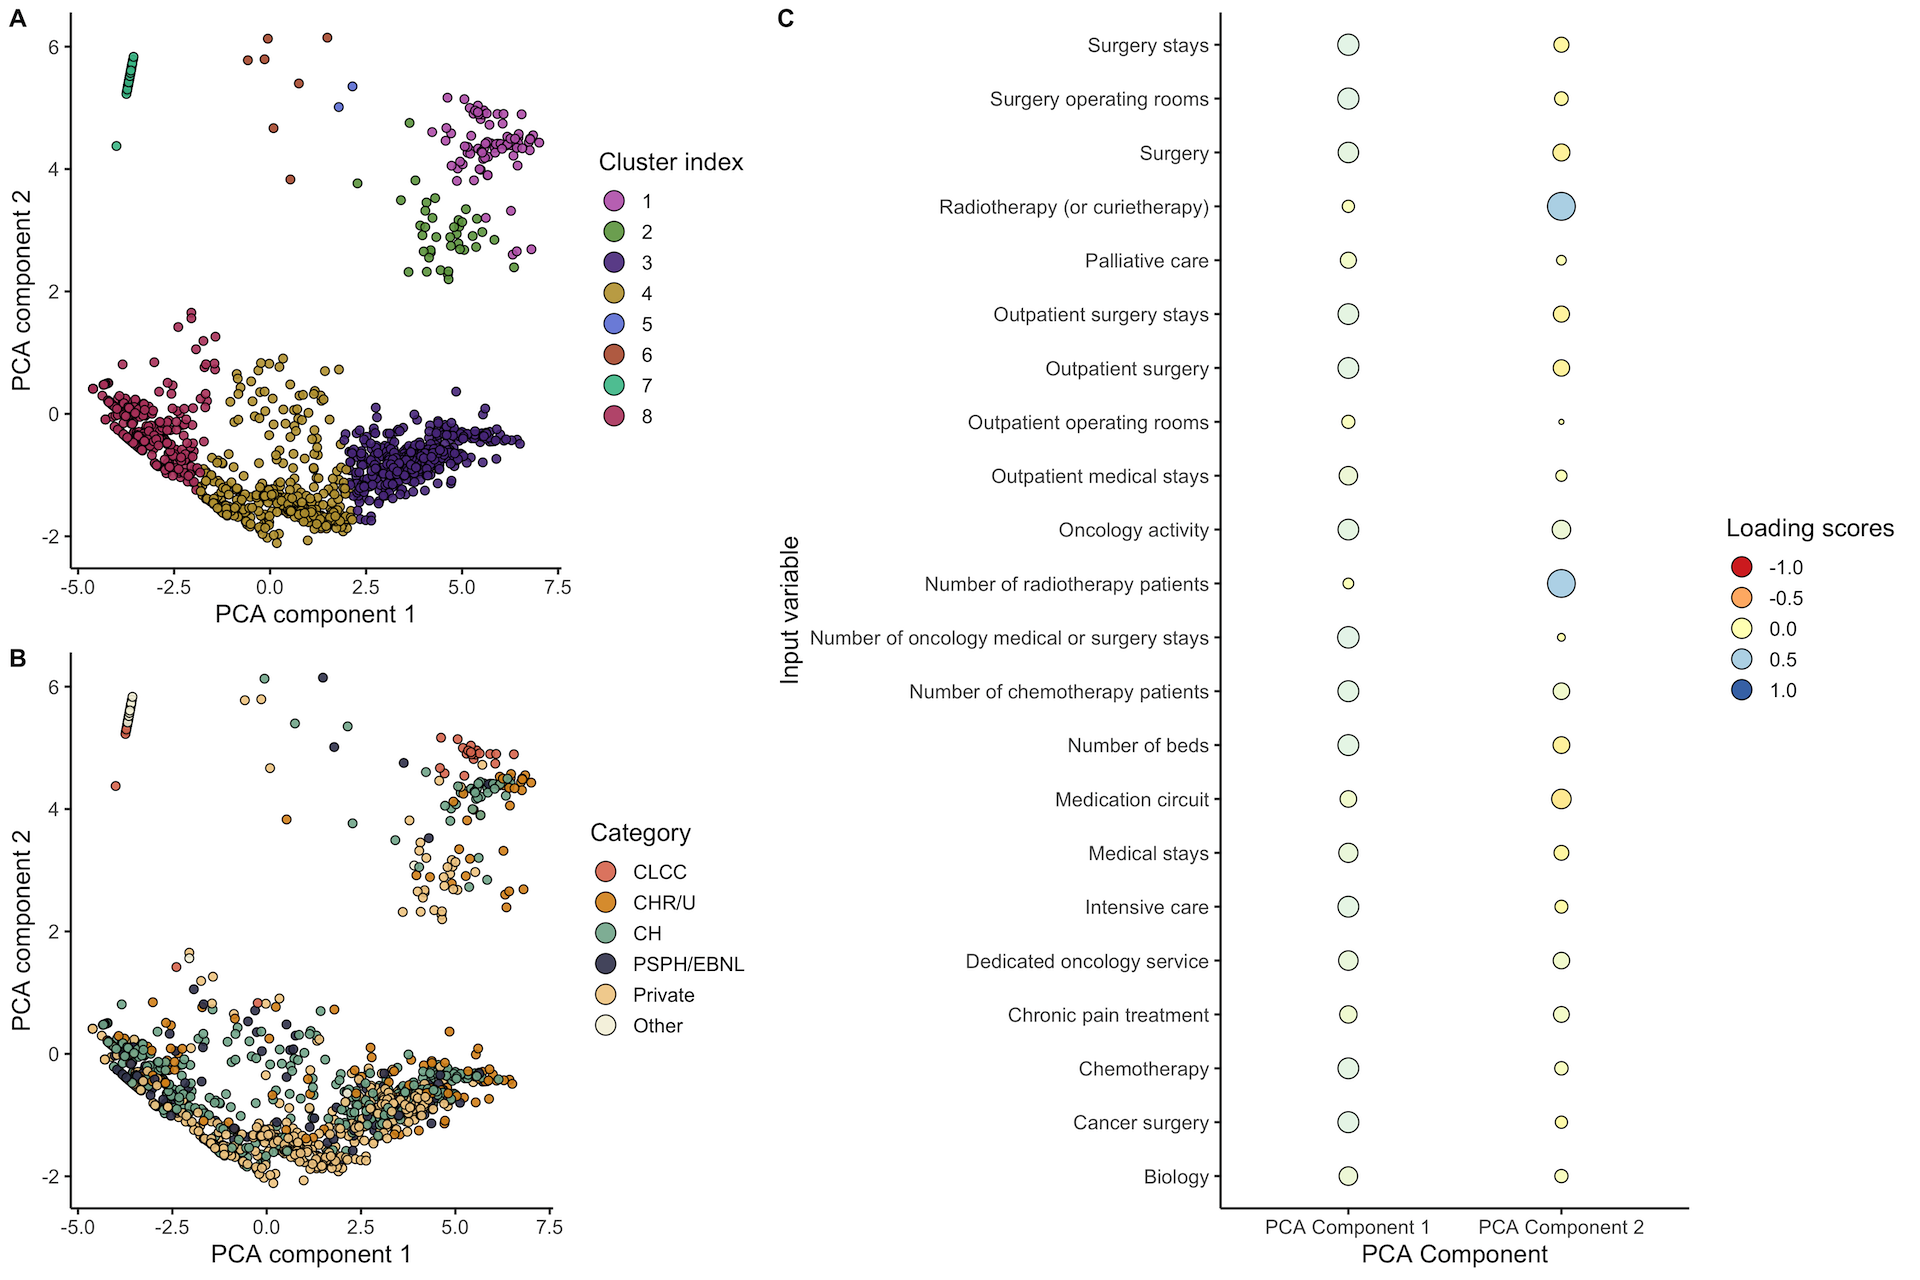
\includegraphics[width=\textwidth]{images/camion/supplemental/sup_fig1_pca_and_clustering.png}
    \centering
    \caption{
        \textbf{\ac{pca} interpretation}. Care centers are showed as points in the 2-dimensional \ac{pca} space. Points are colored by cluster index (A) and hospital type (B). \ac{clcc} care centers are close together in the \ac{pca} space, proving they have similar activity and services distribution. \ac{pca} components are a linear combination of the input variables (C). The loading scores reflect how much the input variable contributed to the \ac{pca} component. Component 1 is associated with most of the variables, while component 2 is linked with radiotherapy variables. Hence, we interpret component 1 as hospital size and component 2 as oncology specialization.
    }
    \label{fig:clustering-pca}
\end{figure}

\section{Results}

In 2018, the population in France was 66,993 million. Mainland France hosts 64,812 million inhabitants (96.8\%), while the remaining 2,181 million (3.2\%) live in overseas departments and regions . Metropolitan France is divided into 13 administrative regions and 96 departments. The population density in France is unevenly distributed . In 2020, the overall population density in metropolitan France was 119 inhabitants per square kilometer. Ile-de-France region has the highest population density with 1,022 inhabitants per square kilometer. Density in other regions in metropolitan France range between 40 and 187 inhabitants/km2. Denser areas are located near the coastline and around the largest cities like Paris, Marseille, Lyon, Strasbourg, Toulouse, or Bordeaux. The middle of the country is rural, and the population densities are low. While there are a great variety of regions and landscapes, the country is becoming more urbanized. This ``rural exodus'' is largely responsible of what is known as the ``empty diagonal'', a band of very low-density population that stretches from the southwest to the northeast.
We now describe the spatial distribution and specificities of the 1,662 hospitals included in this study. There are different types of hospitals in France: \ac{ch}  (n=667) and \ac{chru}  (n=142) are state-run hospitals; \ac{clcc}  (n=26) and \ac{psph}/\ac{ebnl}  (n=142) are both private hospitals of collective interest, though \ac{clcc} are oncology dedicated; private hospitals (n=606) are privately run and for-profit. The non \ac{mco} care centers with radiotherapy activity (n=79) are mostly private practice structures and are referred as “Other”. \cref{table:oncology-activity-per-region} shows the number of care centers and their oncology activity per hospital type and region. Most of the care centers are public, but a non-insignificant part are private. \ac{clcc} represent only 1.6\% of the care centers, yet they are responsible for 14.2\% of the overall oncology activity. The care centers are unevenly distributed across the country. For instance, Corse and Centre-Val-de-Loire are the only two regions with no \ac{clcc} care centers. Moreover, the proportion of oncology activity per hospital type varies from a region to another. For instance, in Nouvelle-Aquitaine, 47.1\% of the oncology activity is handled by private care centers, whereas in Provence-Alpes-Cote-d'Azur it is 21.4\%.

While it is obvious that \ac{clcc} care centers are suited for oncology care, it is difficult to assess the degree of oncology specialization for other care centers. Our clustering algorithm assigns the n=1,662 care centers into 8 clusters, sorted by oncology specialization. \cref{fig:clustering-spider} shows the distribution of some of the key health services per cluster. These services are biology, radiotherapy, chemotherapy, cancer surgery, intensive unit, palliative care, oncology unit, medication circuit, surgery, and outpatient surgery. The three oncology services are cancer surgery, radiotherapy, and chemotherapy. We see that care centers from clusters 1 (n=79) and 2 (n=39) all have these 3 services, hence they are the most suited hospitals for oncology care. Centers from cluster 3 (n=451) have cancer surgery and chemotherapy but lack radiotherapy. The most part of the n=381 centers from cluster 4 have cancer surgery, but no radiotherapy nor chemotherapy. Care centers from cluster 5 (n=2) and cluster 6 (n=7) have radiotherapy and chemotherapy services, but no cancer surgery. Care centers in cluster 7 (n=77) are dedicated to radiotherapy and mostly private practice structures. Finally, care centers 8 (n=626) have none of the 3 oncology services. To sum up, hospitals from clusters 1 and 2 (n=118) are “all-in-one” care centers that provide the most “ideal” oncology care. Centers from clusters 3 and 4 (n=382) provide oncology care but will have to be coordinated with additional structures during the pathways. Hospitals within clusters 5, 6 and 7 (n=86) are not allowed to perform cancer surgery but provide chemotherapy or radiotherapy. The remaining n=626 care centers in cluster 8 are not equipped for oncology care.

\begin{figure}[H]
    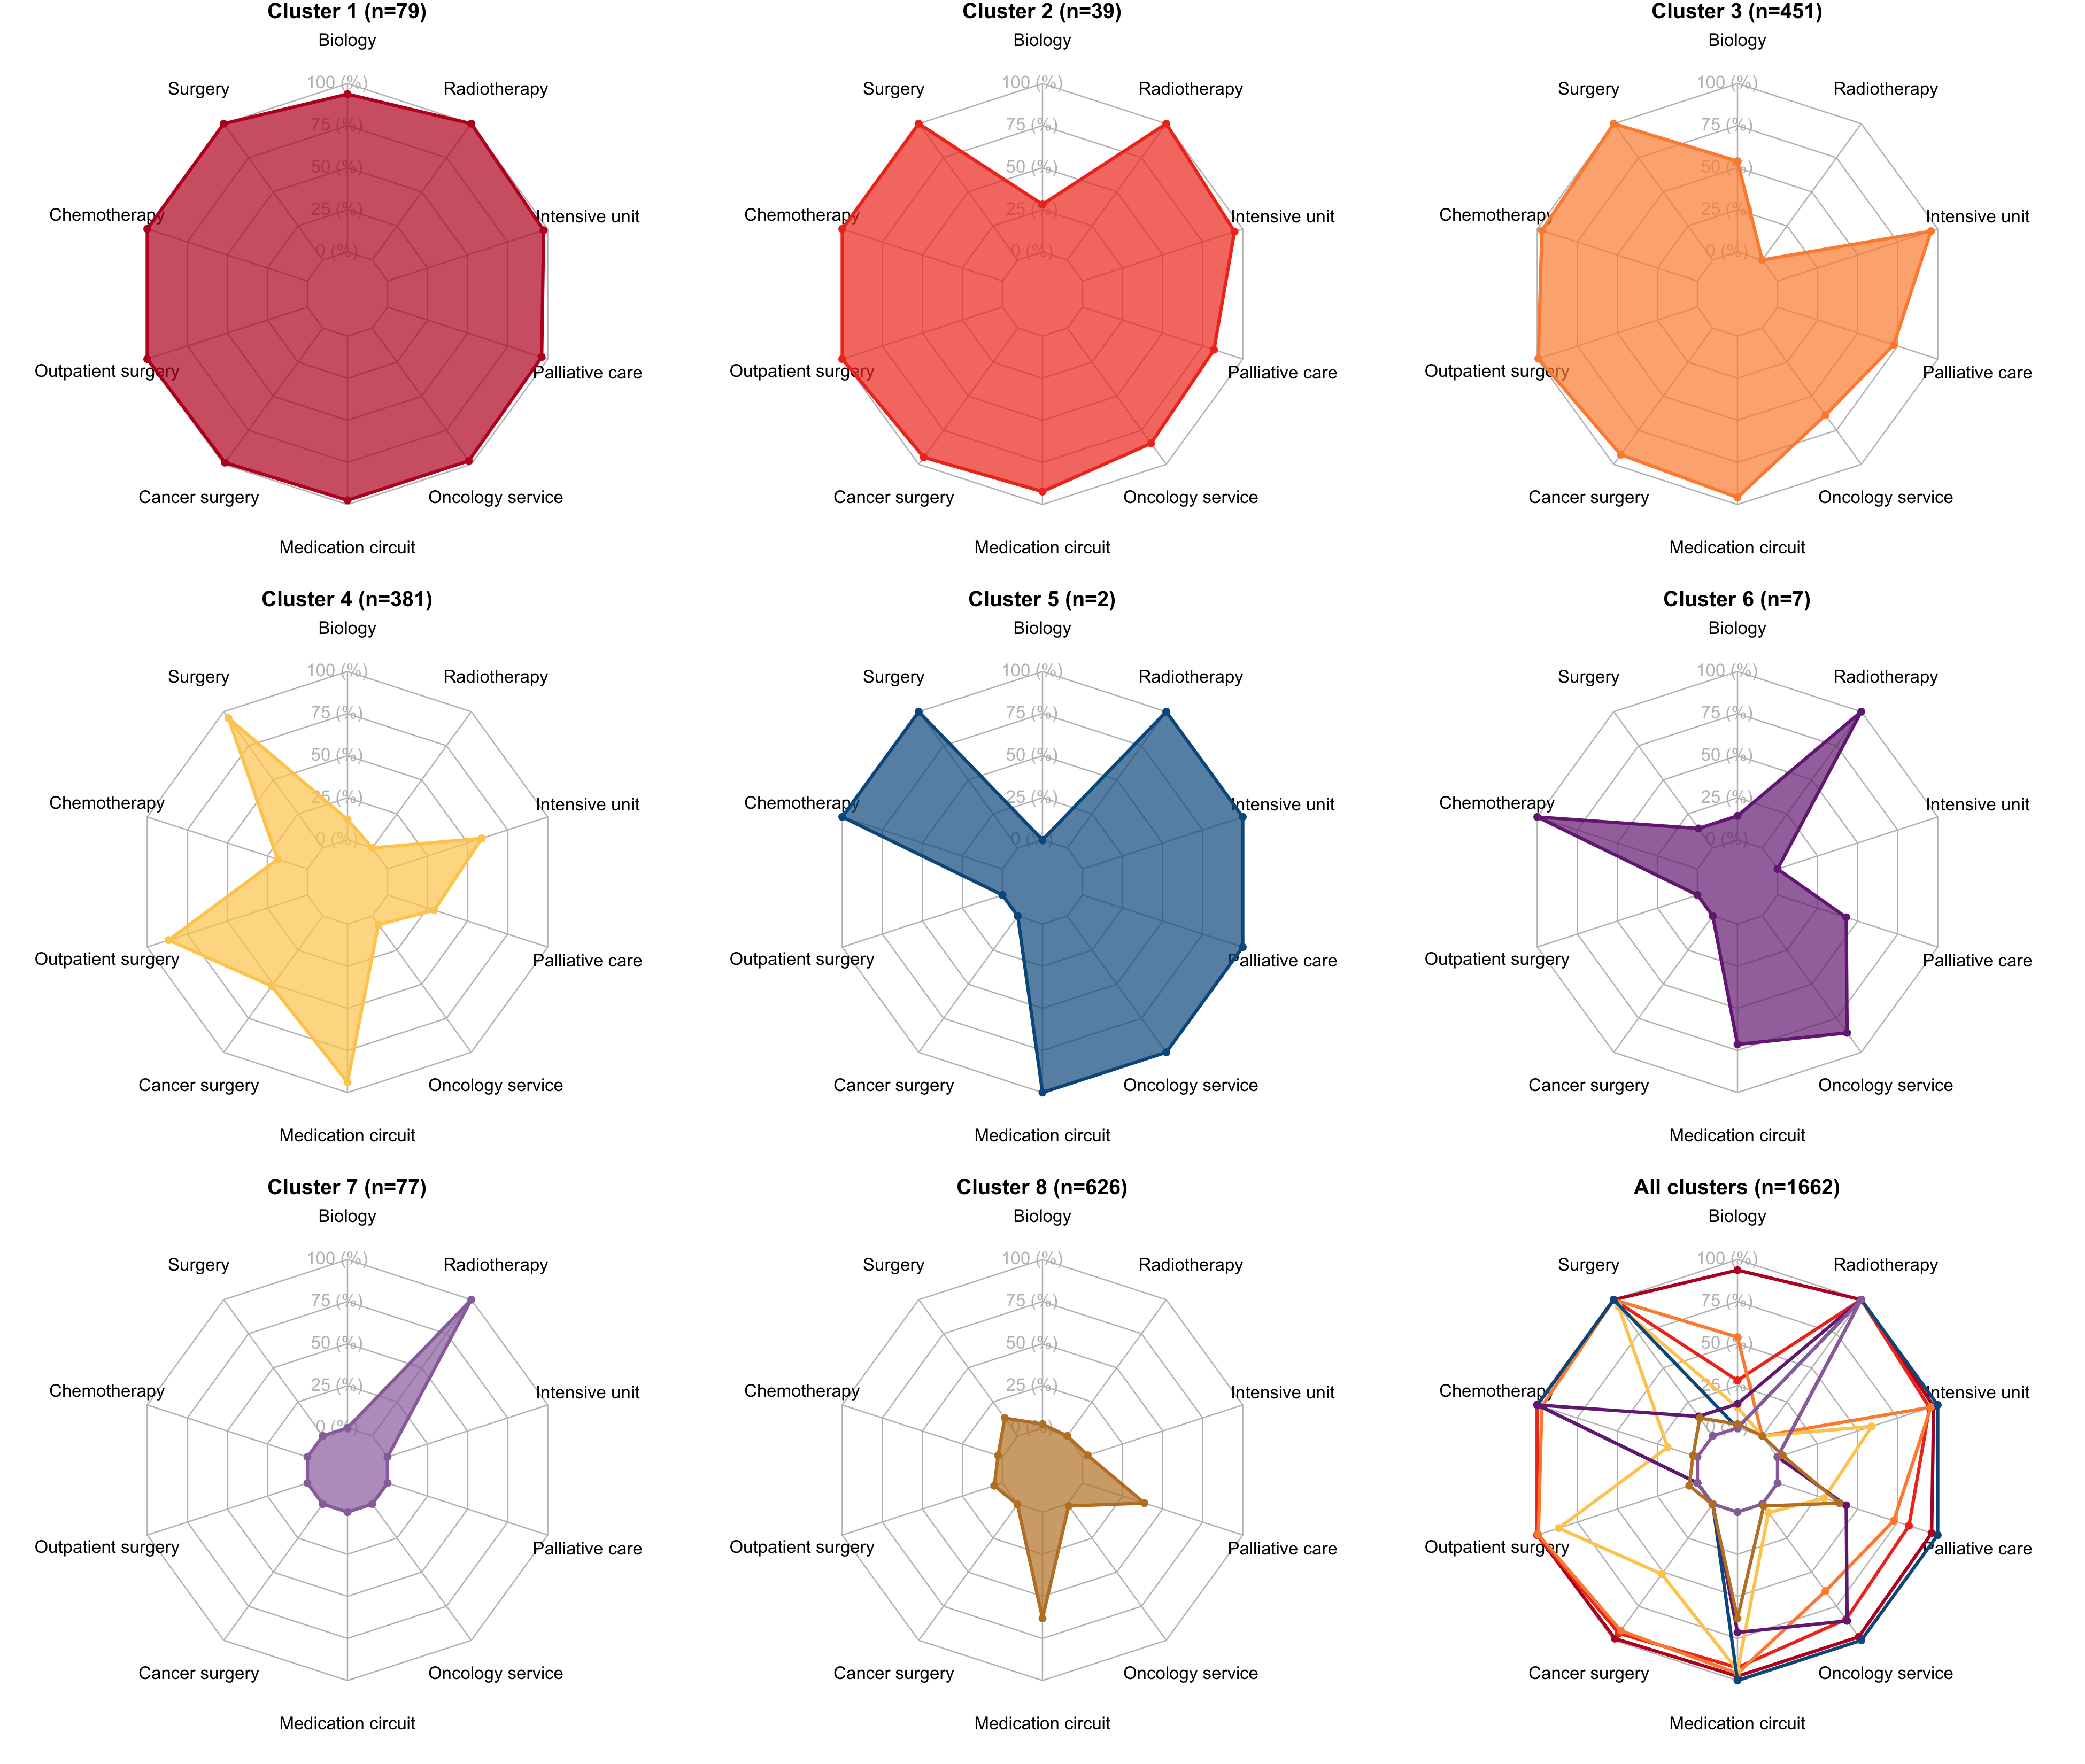
\includegraphics[width=\textwidth]{images/camion/fig1_clusters_services.png}
    \centering
    \caption{
        \textbf{Distribution of the care centers services and equipment per cluster.} Each radar plot axis shows the percentage of the care centers within the cluster that have the corresponding attribute. In Cluster 1, the care centers have all the listed services. In cluster 8, the centers have almost none of the services. Care centers from cluster 1 (n=79) and cluster 2 (n=39) are the most suit-ed for oncology care.
    }
    \label{fig:clustering-spider}
\end{figure}

Hospital types are unevenly distributed among the clusters as illustrated on \cref{fig:clustering-categories}. For instance, 76.9\% of the \ac{clcc} care centers are placed in cluster 1, as they are the most specialized centers. In cluster 7, we find external radiotherapy units of some \ac{clcc} centers, and private practice structures. The proportion of private care centers varies as well: cluster 1 has almost no private care center while cluster 2 has 61.5\% of private hospitals.

\begin{figure}[H]
    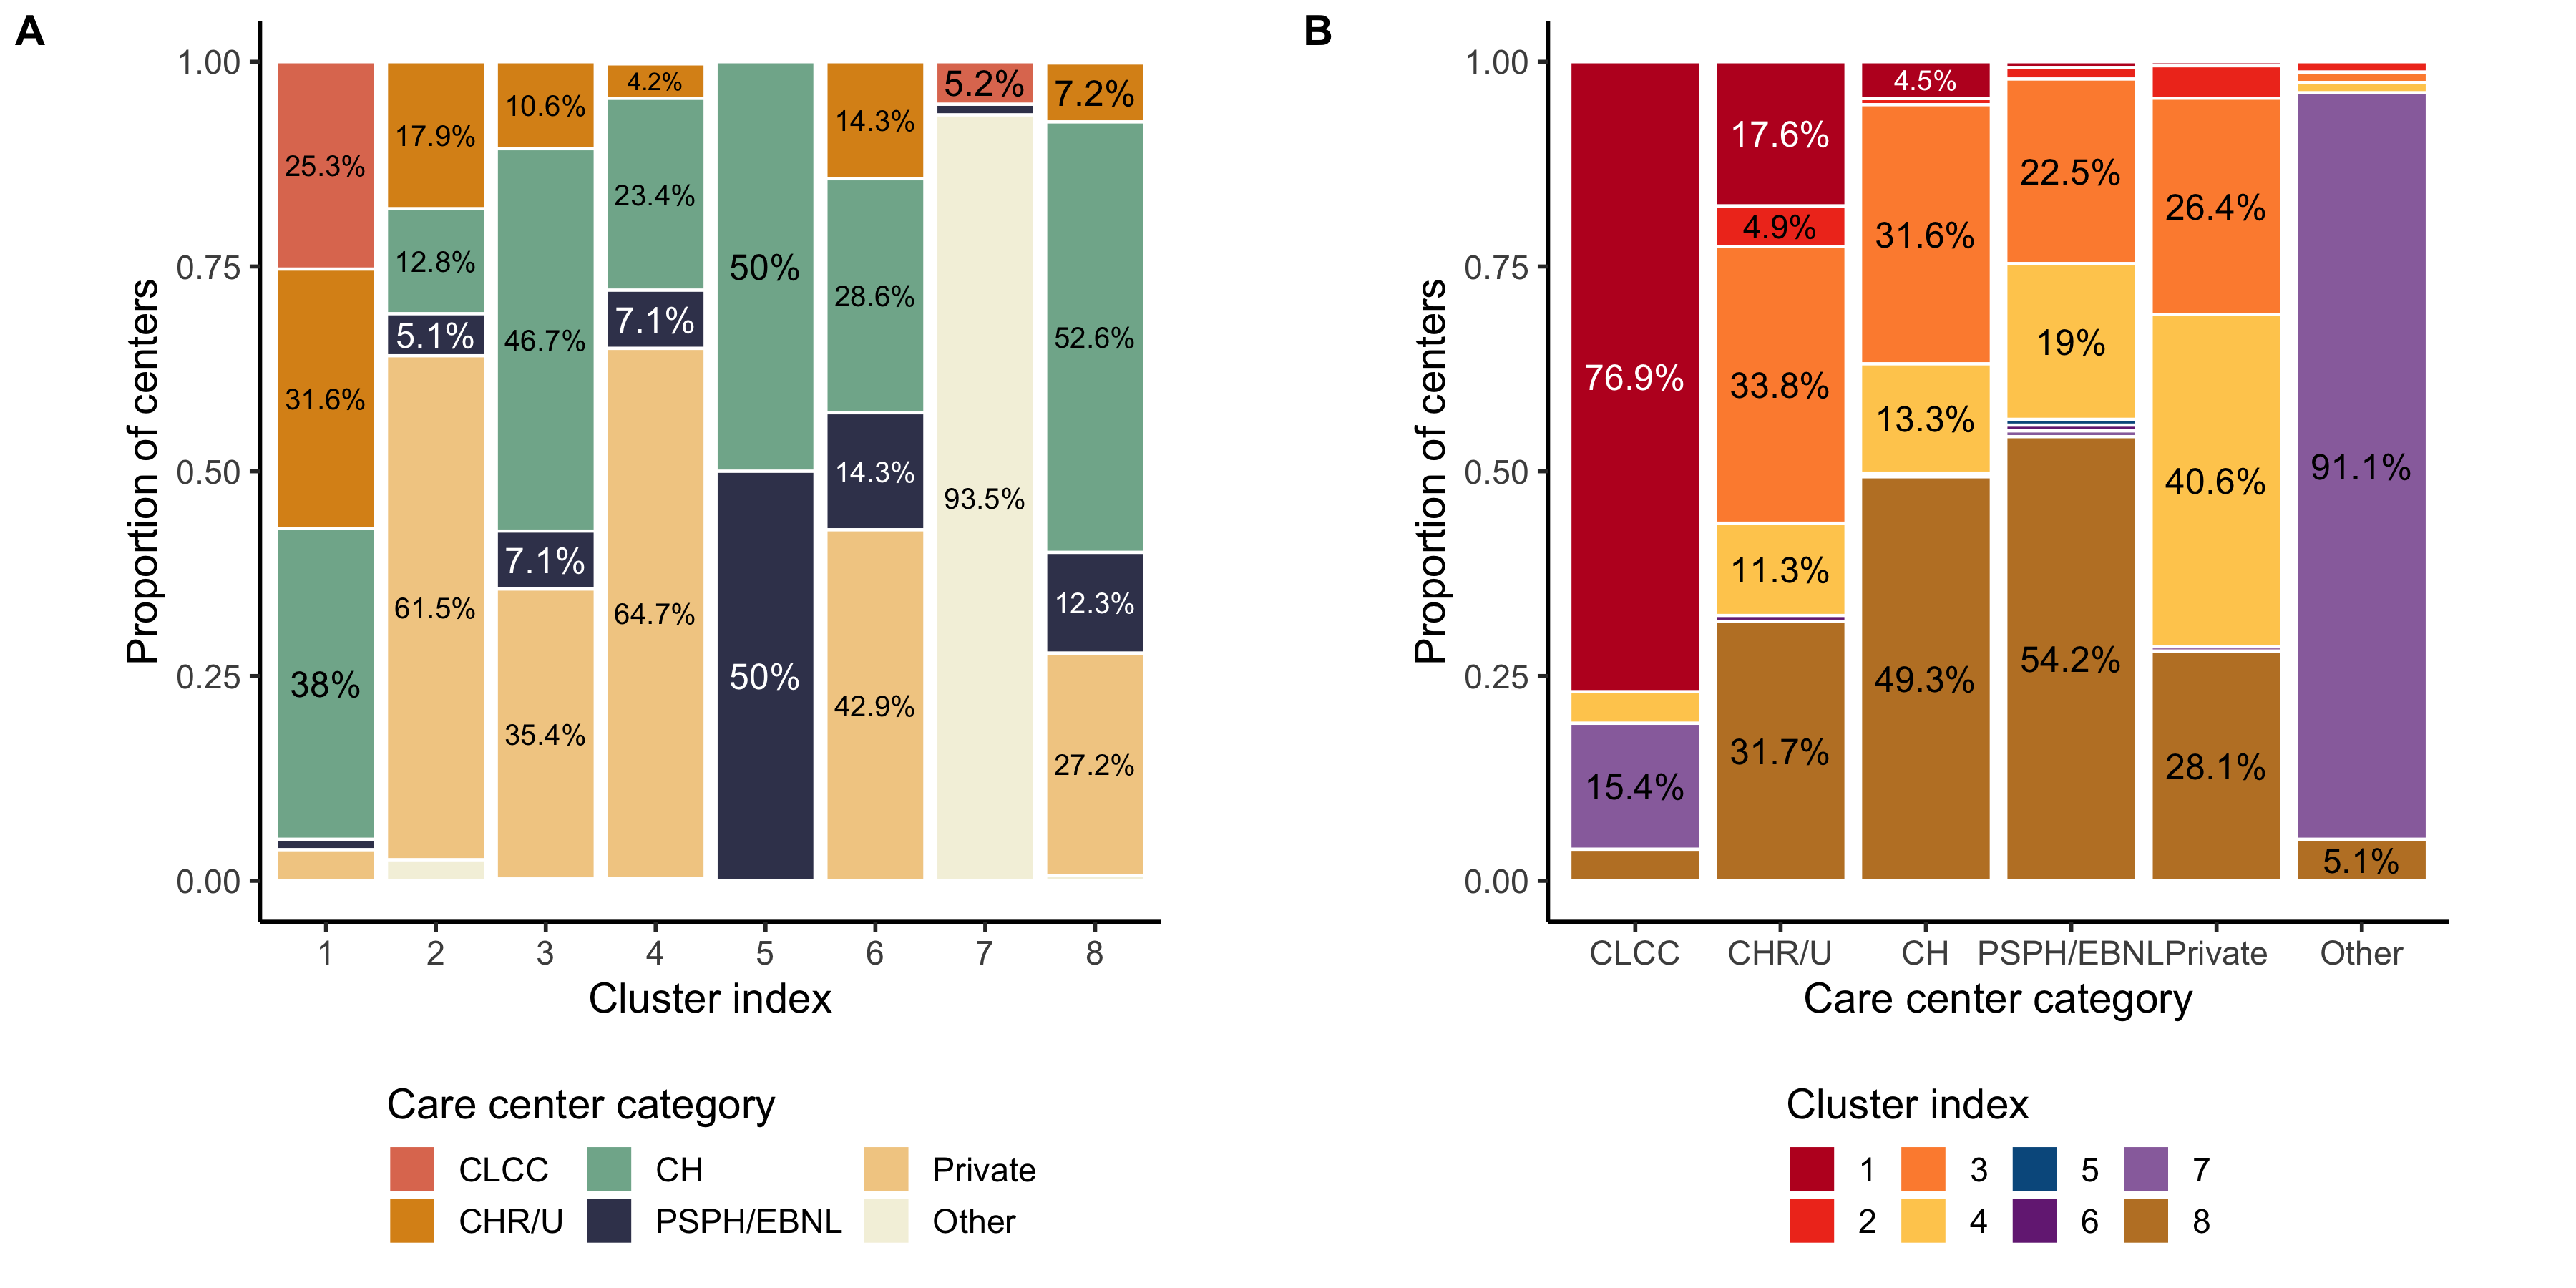
\includegraphics[width=\textwidth]{images/camion/supplemental/sup_fig2_categories_per_cluster.png}
    \centering
    \caption{
        \textbf{Comparison between hospital types and assigned clusters.} The majority of the \ac{clcc} care centers are grouped together in cluster 1. Moreover, cluster 1 has a very low percentage of private hospitals, whereas this proportion is the much higher in cluster 2. “Other” care centers are mostly private practice radiotherapy struc-tures, and they are regrouped in cluster 7.
    }
    \label{fig:clustering-categories}
\end{figure}

Moreover, most of the oncology activity is handled by care centers from clusters 1 and 3, as seen on \cref{fig:clustering-cumulative}. Also, the overall oncology activity from the n=79 centers in cluster 1 is almost as large as the activity of the n=451 hospitals from cluster 4.

\begin{figure}[H]
    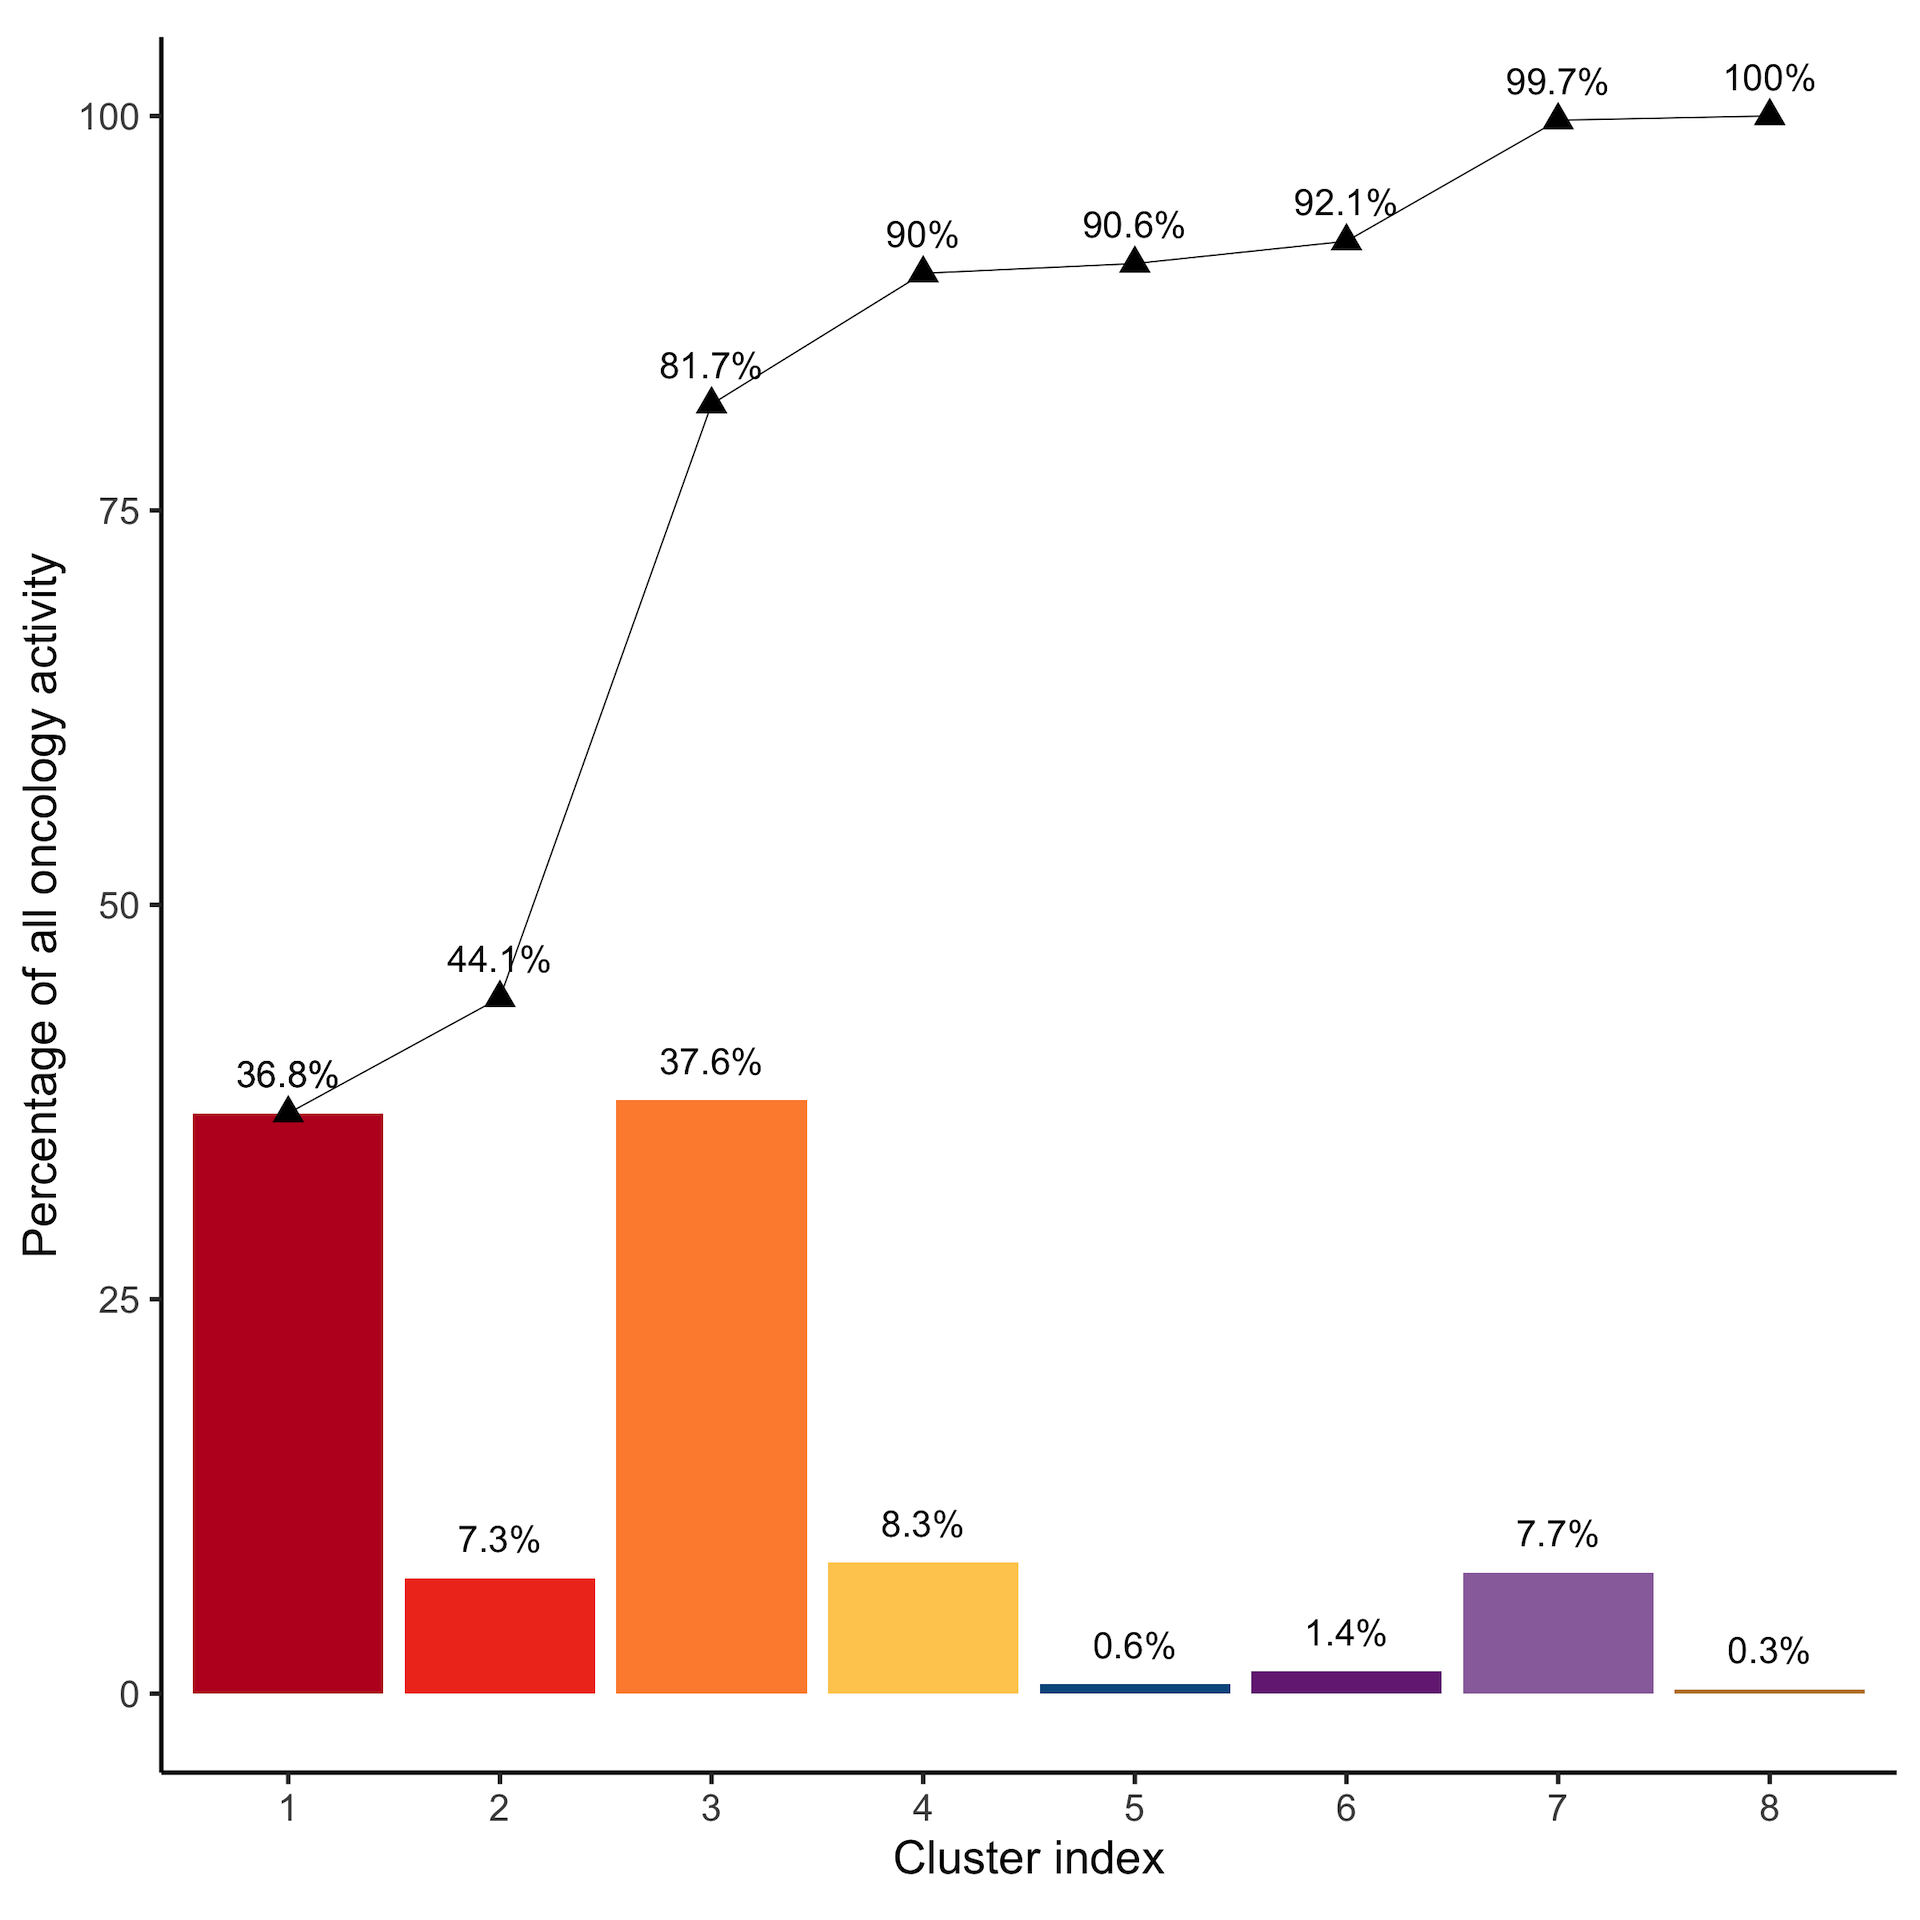
\includegraphics[width=0.5\textwidth]{images/camion/supplemental/sup_fig3_nb_stays_per_cluster.png}
    \centering
    \caption{
        \textbf{Cumulative sum of the oncology activity, per cluster.} Most of the oncology activity is handled by care centers from clusters 1 and 3. While there are only n=79 care centers in cluster 1, their total activity is almost as large as the n=451 care centers from cluster 3.
    }
    \label{fig:clustering-cumulative}
\end{figure}

\begin{figure}[H]
    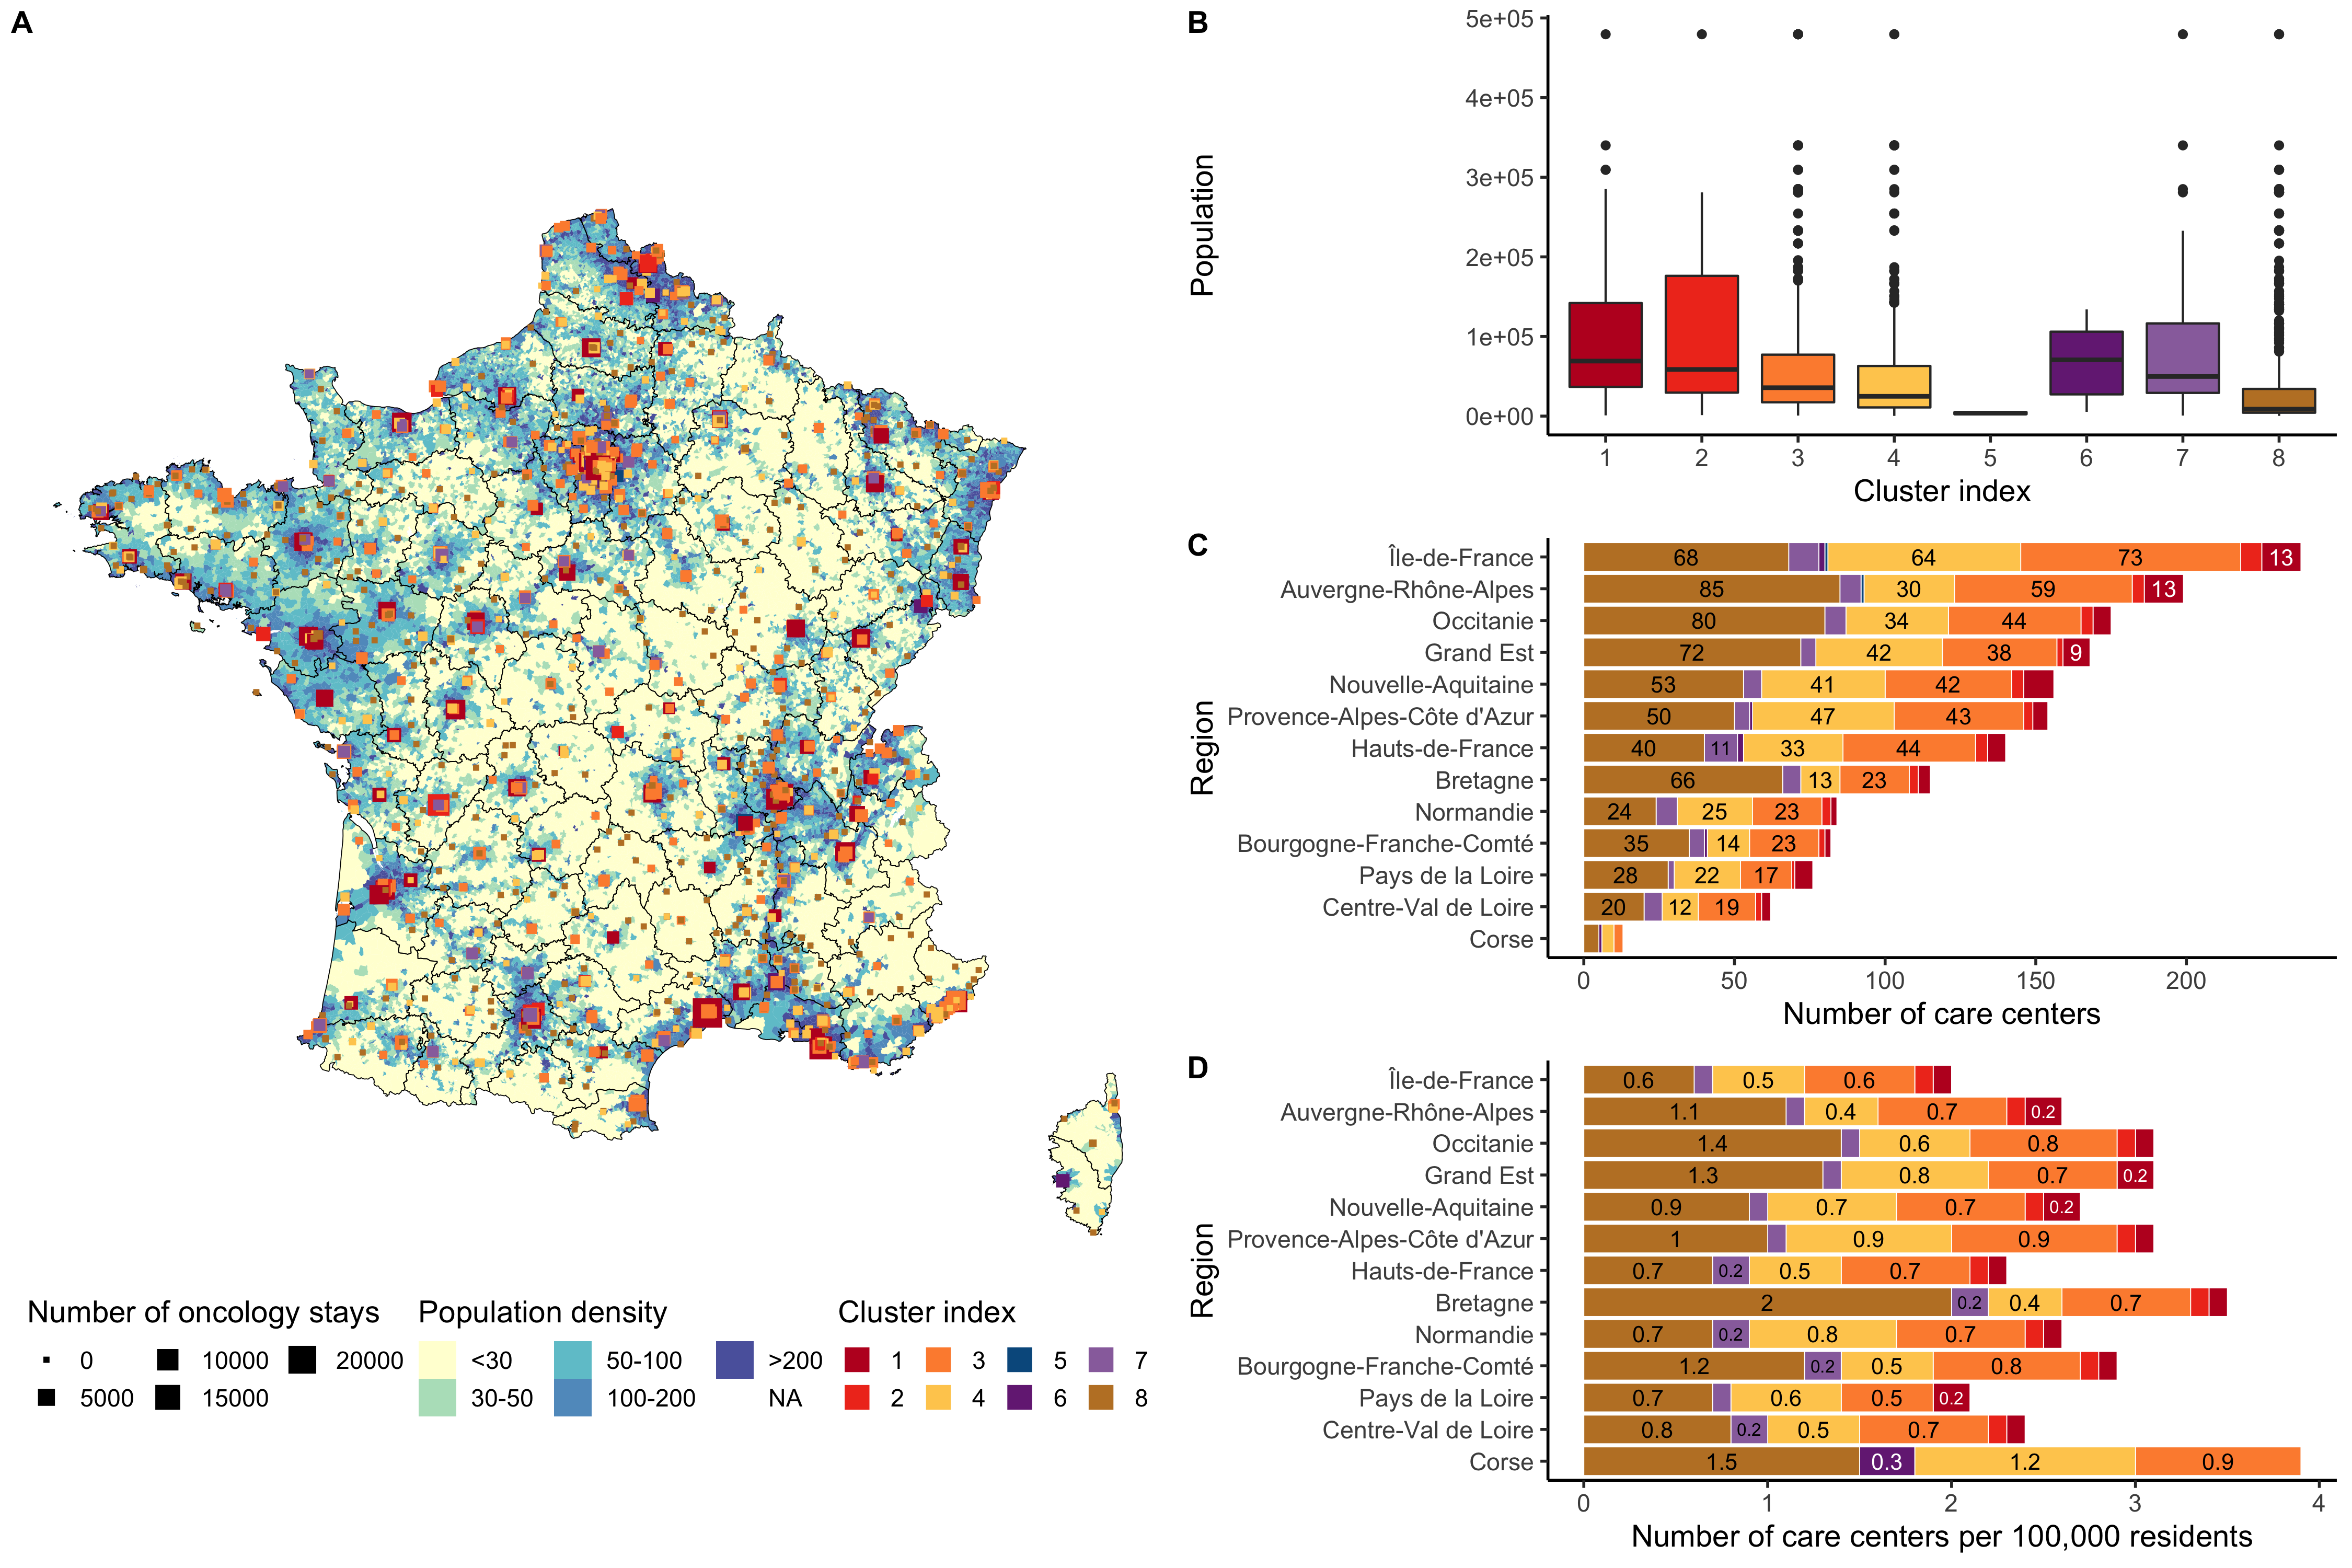
\includegraphics[width=\textwidth]{images/camion/supplemental/sup_fig4_care_centers_pop_density.png}
    \centering
    \caption{
        \textbf{Care centers spatial distribution, compared with population density.} Population density in metropolitan France is unevenly distributed across the country (A). Areas in the middle, near the Pyrenees and the Alps have very low population densities. The most specialized care centers are in dense areas and in large municipalities (B). While Ile-de-France has the highest number of care centers, it has the least care centers per 100,000 inhabitants.
    }
    \label{fig:clustering-map}
\end{figure}

\begin{table}[H]
    \resizebox{\textwidth}{!}{%
    \begin{tabular}{|l|l|l|l|l|l|l|l|l|}
    \hline
        Variable value per region & ~ & \multicolumn{7}{c}{Hospital Type} \\ \hline
        N = number of centers & ~ & \acs{ch} & \acs{ch} & \acs{clcc} & Other & \acs{psph}/\acs{ebnl} & Privé & All \\
        A = oncology activity (radio. + chemo. + surgery) & ~ &  (n=667)  & (n=142) & (n=26) & (n=79) & (n=142) & (n=606) & n=1,662 \\ \hline
        Auvergne-Rhône-Alpes & N & 98 (49,2\%) & 21 (10,6\%) & 2 (1\%) & 7 (3,5\%) & 13 (6,5\%) & 58 (29,1\%) & 199 \\
        ~ & A & 34,597 (26,7\%) & 31,706 (24,5\%) & 16,966 (13,1\%) & 6,710 (5,2\%) & 6,146 (4,7\%) & 33,297 (25,7\%) & 129.422 \\ \hline
        Bourgogne-Franche-Comté & N & 53 (64,6\%) & 4 (4,9\%) & 1 (1,2\%) & 5 (6,1\%) & 2 (2,4\%) & 17 (20,7\%) & 82 \\
        ~ & A & 12,238 (27,6\%) & 10,621 (24\%) & 5,844 (13,2\%) & 4,405 (9,9\%) & 657 (1,5\%) & 10,571 (23,8\%) & 44.336 \\ \hline
        Bretagne & N & 38 (33\%) & 8 (7\%) & 1 (0,9\%) & 6 (5,2\%) & 11 (9,6\%) & 51 (44,3\%) & 115 \\
        ~ & A & 15,953 (27\%) & 11,020 (18,6\%) & 6,341 (10,7\%) & 5,553 (9,4\%) & 2,050 (3,5\%) & 18,199 (30,8\%) & 59.116 \\ \hline
        Centre-Val de Loire & N & 29 (46,8\%) & 4 (6,5\%) & 0 (0\%) & 6 (9,7\%) & 2 (3,2\%) & 21 (33,9\%) & 62 \\
        ~ & A & 6,989 (19,6\%) & 11,524 (32,2\%) & 0 (0\%) & 5,137 (14,4\%) & 32 (0,1\%) & 12,058 (33,7\%) & 35.74 \\ \hline
        Corse & N & 7 (53,8\%) & 0 (0\%) & 0 (0\%) & 0 (0\%) & 0 (0\%) & 6 (46,2\%) & 13 \\
        ~ & A & 3,486 (66,3\%) & 0 (0\%) & 0 (0\%) & 0 (0\%) & 0 (0\%) & 1,773 (33,7\%) & 5.259 \\ \hline
        Grand Est & N & 70 (41,7\%) & 17 (10,1\%) & 3 (1,8\%) & 6 (3,6\%) & 30 (17,9\%) & 42 (25\%) & 168 \\
        ~ & A & 17,428 (19,6\%) & 22,123 (24,9\%) & 13,176 (14,8\%) & 6,793 (7,7\%) & 7,683 (8,7\%) & 21,553 (24,3\%) & 88.756 \\ \hline
        Hauts-de-France & N & 56 (40\%) & 11 (7,9\%) & 1 (0,7\%) & 11 (7,9\%) & 12 (8,6\%) & 49 (35\%) & 140 \\
        ~ & A & 21,864 (26\%) & 15,934 (19\%) & 6,947 (8,3\%) & 8,618 (10,3\%) & 5,242 (6,2\%) & 25,399 (30,2\%) & 84.004 \\ \hline
        Île-de-France & N & 40 (47,6\%) & 5 (6\%) & 4 (4,8\%) & 6 (7,1\%) & 3 (3,6\%) & 26 (31\%) & 84 \\
        ~ & A & 7,573 (14,9\%) & 7,947 (15,7\%) & 14,210 (28\%) & 5,419 (10,7\%) & 0 (0\%) & 15,627 (30,8\%) & 50.776 \\ \hline
        Normandie & N & 70 (44,9\%) & 10 (6,4\%) & 1 (0,6\%) & 7 (4,5\%) & 12 (7,7\%) & 56 (35,9\%) & 156 \\
        ~ & A & 37,844 (33\%) & 26,244 (22,9\%) & 7,477 (6,5\%) & 7,157 (6,2\%) & 2,824 (2,5\%) & 33,271 (29\%) & 114.817 \\ \hline
        Nouvelle-Aquitaine & N & 66 (37,7\%) & 14 (8\%) & 2 (1,1\%) & 7 (4\%) & 6 (3,4\%) & 80 (45,7\%) & 175 \\
        ~ & A & 14,735 (12,1\%) & 20,915 (17,2\%) & 16,047 (13,2\%) & 11,572 (9,5\%) & 1,098 (0,9\%) & 57,374 (47,1\%) & 121.741 \\ \hline
        Occitanie & N & 34 (44,7\%) & 5 (6,6\%) & 3 (3,9\%) & 4 (5,3\%) & 5 (6,6\%) & 25 (32,9\%) & 76 \\
        ~ & A & 11,901 (18,9\%) & 11,374 (18,1\%) & 12,564 (19,9\%) & 3,422 (5,4\%) & 3,916 (6,2\%) & 19,822 (31,5\%) & 62.999 \\ \hline
        Pays de la Loire & N & 53 (34,4\%) & 10 (6,5\%) & 3 (1,9\%) & 4 (2,6\%) & 15 (9,7\%) & 69 (44,8\%) & 154 \\
        ~ & A & 14,632 (13,6\%) & 16,533 (15,4\%) & 21,924 (20,4\%) & 6,172 (5,7\%) & 10,918 (10,2\%) & 37,176 (34,6\%) & 107.355 \\ \hline
        Provence-Alpes-Côte d'Azur & N & 53 (22,3\%) & 33 (13,9\%) & 5 (2,1\%) & 10 (4,2\%) & 31 (13\%) & 106 (44,5\%) & 238 \\
        ~ & A & 24,390 (12,6\%) & 66,406 (34,2\%) & 34,028 (17,5\%) & 12,817 (6,6\%) & 14,981 (7,7\%) & 41,577 (21,4\%) & 194.199 \\ \hline
        Grand Total & N & 667 (40,1\%) & 142 (8,5\%) & 26 (1,6\%) & 79 (4,8\%) & 142 (8,5\%) & 606 (36,5\%) & 1662 \\
        ~ & A & 223,630 (20,4\%) & 252,347 (23\%) & 155,524 (14,2\%) & 83,775 (7,6\%) & 55,547 (5,1\%) & 32,7697 (29,8\%) & 1,098,520 \\ \hline
    \end{tabular}}
    \caption{
        \textbf{Number of care centers (N) and overall oncology activity (A) per hospital type and region.} Oncology activity is the sum of the number of patients with radiotherapy or chemotherapy, and the number of medical or surgery stays related to cancer. \ac{ch} and \ac{ch} are public hospitals; \ac{clcc} and \ac{psph}/\ac{ebnl} are private hospitals of collective interest, though \acs{clcc} are oncology dedicated; private hospitals are for-profit. “Other” hospitals are mostly private practice radiotherapy structures. The percentages sum to 100\% row-wise. In Nouvelle-Aquitaine, 47.1\% of the oncology activity is handled by private care centers, whereas in Provence-Alpes-Cote-d’Azur it is 21.4\%.
    }
    \label{table:oncology-activity-per-region}
\end{table}

\section{Discussion}

The clustering algorithm successfully groups similar hospitals and lets us identify the care centers best suited for oncology care. Some variables in the \ac{sae} survey are declarative and potentially differ from the reality. We are aware of this bias, but we do not expect major differences that could distort our clustering results.
Receiving treatment in a care center with surgery, chemotherapy and radiotherapy activities is easier for the patient and leads to better care pathways. Care centers from cluster 1 will be the better choice for cancer treatment and correspond to modern oncology care specifications. However, these centers are a minority and sparsely located, essentially in dense areas and in large cities. While the inhabitants of large cities and metropolitan areas will have no problem reaching them, rural areas residents live far away from these centers. This population often has better access to care centers from intermediate clusters. Such centers do not have all the key services and the patients are more likely to visit multiple hospitals during their care pathways.
Longer drives to reach a more specialized care center could be considered more acceptable for surgery, where the hospital volume and surgeon expertise matter. However, for more frequent interventions like chemotherapy and radiotherapy especially, patients should prioritize short travels. There is a tradeoff to be found by patients, between care center proximity and care center expertise. This dilemma will be more frequent for patients living in rural areas than patients living in dense cities with large care centers nearby.


  \chapter{Accessibility to oncology care}

\section{Motivation}

While a lot of the ongoing research is focusing on finding new cancer
treatments, accessibility to oncology care receives less attention. Yet, several
studies have showed that access to health services plays a key role in cancer
survival. For instance, geographic residency status and social environment seem
to explain treatment and prognosis disparities for patients with non-small cell
lung cancer \cite{johnson_treatment_2014}. In France, increases in travel times
to health services were associated with lower survival rates for patients with a
colorectal cancer \cite{dejardin_influence_2014}. In New Zealand, living in
deprived areas, far from a cancer center or from primary care was associated
with lower survival chances for patients with colorectal, lung and prostate
cancers \cite{haynes_cancer_2008}.

Accessibility refers to the relative ease by which services can be reached from
a given location \cite{wang_measurement_2012}. Accessibility can be defined by
spatial factors, determined by where you are; and non-spatial factors,
determined by who you are \cite{khan_integrated_1992}. In what follows, we
restrict accessibility to \acf{sa} and use both terms interchangeably. \ac{sa}
methods assess the availability of supply locations from demand locations,
connected by a travel impedance metric. Supply locations are characterized by
their capacity or quantity of available resource. Similarly, demand locations
are characterized by their population. Such methods have been successfully used
to measure access to healthcare, such as primary care
\cite{guagliardo_spatial_2004} or oncology care
\cite{wang_measurement_2012,zahnd_spatial_2021,alahmadi_spatial_2013} in several
countries including France
\cite{launay_methodology_2019,gusmano_disparities_2014,gao_assessment_2016}.
When measuring accessibility for healthcare, the supply locations are often
physicians locations, whose capacity might be the number of physicians at that
location. Population locations represent where patients live. This could be
the precise address or a municipality. However, while accessibility to primary
care have been described in several studies, there is little work that focused
on oncology care specifically. In what follows, we applied \ac{sa} methods to
quantify the accessibility the oncology care in metropolitan France.
Intuitively, we compute a score for every municipality that measures how easy
it would be for patients living in a given municipality to reach oncology care.

\section{Methods}

\subsection{\acf{sa} methods overview}

There are several ways to compute accessibility to healthcare as reviewed in
\cite{guagliardo_spatial_2004}. Some methods are very straightforward and as
easy as computing ratios per geographical units. Other methods are more
sophisticated and can model more real world factors. We detail these methods in
the following sections.

\subsubsection{Provider-to-population ratios}

The easiest and most straightforward \ac{sa} method is to compute
provider-to-population ratios, also referred as supply ratios. The ratio
involves some indicator of health service capacity (supply) as numerator; while
the denominator is the population size within the area (demand). For instance,
when measuring accessibility to primary care, one might use the number of
physicians in the area as supply, and area population as demand. The resulting
ratio might be interpreted as the number of physicians per 100,000 inhabitants
\cite{schonfeld_numbers_1972}.

Supply ratios are highly interpretable, and relevant for comparisons of supply
in large areas. Policy analysts have used these metrics to set minimal standards
of supply and identify under-served areas where supply should be increased
\cite{schonfeld_numbers_1972,council_on_graduate_medical_education_physician_1998,connor_competition_1995}% Cons
However, supply ratios have limitations that often prevent their usage in more
detailed analysis. First, they do not account for patient border crossing, which
commonly occurs for small areas
\cite{connor_measuring_1994,basu_border-crossing_1996,basu_medicare_1995,holahan_border_1993}.
Second, supply ratios are constant within the bordered area, which will lead to
imprecision and false generalization in large areas. Finally, they do not
consider travel impedance, which plays a major role in \ac{sa}. Consequently the
results and interpretations can vary greatly depending on the size, number and
configuration of the areal units studied. This problem is well-known to
geographers and spatial analysts as the modifiable areal unit problem (MAUP)
\cite{openshaw_modifiable_1983}.

\subsubsection{Travel impedance to providers}

As stated earlier, travel impedance is a key aspect of \ac{sa} evaluation. It is
typically measured from a patient's residence or from the centroid of a
population location when the precise location is not available. The impedance
can be expressed in different ways: euclidean (straight) distance, travel
distance or estimated travel time.

Travel impedance is suited for rural areas, where providers are limited and
patients often travel to the nearest choice available. However, travel impedance
is less relevant for urban areas. Indeed, there are numerous reasonable options
available at a similar distance and patients won't travel to the closest one
anymore. Moreover, travel impedance is a poor indicator of availability and
should be combined with supply to properly evaluate \ac{sa}
\cite{fryer_multi-method_1999}.

\subsubsection{Gravity models}

Gravity models are more sophisticated ways to evaluate \ac{sa}, based on a
modified version of Newton's Law of Gravitation. They were initially developed
to predict retail travel \cite{reilly_law_1931} and help with land use planning
\cite{hansen_how_1959}. Gravity models combine both accessibility and
availability, and work well in urban and rural settings. Gravity models
represent the influence of all service points located within a reasonable
distance from a population location. The influence is discounted by the
increasing distance or travel impedance. The simplest formula for gravity-based
accessibility is:

\begin{equation}
    A_i = \sum_j \frac{S_j}{d_{ij}^{\beta}}
\end{equation}

In this equation, $A_i$ is the accessibility score at population location $i$.
$S_u$ is the capacity of the service point $u$, and $d_{iu}$ the travel
impedance (e.g. distance or travel time) between population location $i$ and
service point $u$. We set $\beta$ as a gravity decay coefficient, sometimes
referred to as the travel friction coefficient. Intuitively, $\beta$ represents
the change in difficulty of travel as the impedance value increases. The
accessibility score increases with higher provider capacity, and decreases with
higher travel impedance. Gravity models are an elegant way to compute
accessibility, which accounts for border crossing, local variations, and travel
impedance. The main drawbacks of this approach is the lack of intuitiveness, and
healthcare policy makers prefer to think of \ac{sa} in terms of
provider-to-population ratios or simple distance. Second, it only models supply
and does not account for demand. Providers should not be equally accessible if
they serve population locations with drastically different population sizes. A
proposed solution is to add a population demand factor $V_u$, to the denominator
\cite{joseph_measuring_1982}:

\begin{equation}
    V_u = \sum_k \frac{P_k}{d_{ku}^{\beta}}
\end{equation}

Here, $P_k$ is the population size at population location $k$, and $d_{ku}$ is
the distance between the population location $k$ and provider location $u$.
Intuitively, the demand on provider location $u$ is obtained by summing the
gravity discounted influence of all population points within a reasonable
distance. The improved gravity model is:

\begin{equation}
    A_i = \sum_j \frac{S_j}{d_{ij}^{\beta} V_j}
\end{equation}

However, another problem is that the distance decay coefficient, $\beta$, is
usually unknown and hard to estimate. Its form and magnitude can vary greatly
with the service type and population under study \cite{talen_assessing_1998}.

\subsubsection{\acf{2sfca}}

Recently, a new type of method has been developed and is now used in most
\ac{sa} papers. This algorithm is called \acf{2sfca} \cite{luo_using_2004}. It is
a two-step method that first computes a provider-to-population ratio for each
provider location. In the second step, for each population location, an
accessibility score is obtained by summing the provider-to-population ratios.
For the algorithm to work, a catchment threshold (distance or travel time) must
be set. Above this threshold, a provider location is considered unreachable from
the population location, and vice versa.

\begin{itemize}
    \item Step 1: for every care center $u$, compute its
          capacity-to-population ratio $R_u$.
    \item Step 2: for every population location, compute $A_i$ as the sum all
          the $R_u$ of the reachable providers.
\end{itemize}

\begin{align}
    R_u & =  \frac{S_u}{ \sum_{k \in \{ d_{ku} \leq d_0 \}  } P_k } \\
    A_i & = \sum_{u \in \{ d_{iu} \leq d_0 \} } R_u
\end{align}

The capacity of a provider is balanced by the total population with access to
it. A population location that solely has access to low capacities or
overcrowded providers will have a low accessibility score. Similarly, a
population location will have low accessibility scores if the distance to get to
the nearby providers is above the catchment area.

\subsubsection{\acf{e2sfca}}

The \ac{2sfca} method does not account for distance decay: a provider is either
reachable or not. The \ac{e2sfca} \cite{luo_enhanced_2009} addresses this
limitation by applying weights to differentiate travel zones in both steps.
Consider $P_i$ the population at location $i$, with $1 \leq i \leq n$ where $n$
is the number of population locations. Similarly, consider $S_u$ the capacity of
care center $u$, with $1 \leq u \leq m$ where $m$ is the number of care centers.
Finally, let $d_{iu}$ be the matrix of size $n \times m$ containing the
distances between location $i$ and providers $u$. We consider $r$ sub-catchment
zones each associated with a weight $W_s$, and a distance $D_s$, with $1 \leq s
    \leq r$, such that $D_1 < D_2 < ... < D_r$ and $W_1 > W_2 > ... > W_r$. The
resulting r travel intervals are $I_1=[0, D_1], I_2=[D_1, D_2 ], ...
    ,I_r=[D_{r-1}-,D_r]$. The accessibility $A_i$ of a population location $i$ is
computed in two steps:

\begin{itemize}
    \item Step 1: for every care center $u$, compute its weighted
          capacity-to-population ratio $R_u$.
    \item Step 2: for every population location, compute $A_i$ as the sum all
          the weighted $R_u$ of the reachable providers.
\end{itemize}

\begin{align}
    R_u & =  \frac{S_u}{\sum_{s=1}^{r} W_s \sum_{i, d_{iu} \in I_s} P_i} \\
    A_i & = \sum_{s=1}^{r} W_s \sum_{u, d_{iu} \in I_s} R_u
\end{align}

\subsubsection{Multi modal \acl{2sfca}}

The \ac{e2sfca} methodology can be enhanced by incorporating both public and
private transport modes \cite{langford_multi-modal_2016}. The proposed model
yields separate accessibility scores for each modal group at each demand point
to better reflect the differential accessibility levels experienced by each
cohort.

Suppose that each method of travel (car, bus, walking, etc.) necessitates a
dedicated transport network and let each such network be referred to as $N_1,
    N_2, ..., N_M$. In order to accommodate independent networks for each travel
mode into the \ac{e2sfca} model, the computation of Step 1 becomes:

\begin{equation}
    R_u =  \frac{S_u}{\sum_{m=1}^{M} \sum_{s=1}^{r} W_{s,m} \sum_{i, d_{iu,m} \in I_s} P_{i,m}} \\
\end{equation}

Similarly for Step 2:

\begin{equation}
    A_i = \sum_{m=1}^{M} \sum_{s=1}^{r} W_{s, m} \sum_{u, d_{iu} \in I_s} R_u
\end{equation}

\subsubsection{Huff model and \acl{2sfca}}

The \ac{e2sfca} does not consider competition among multiple healthcare sites
available for a population location \cite{wan_three-step_2012}, and therefore it
may lead to overestimation for some sites \cite{luo_integrating_2014}. The Huff
Model is a widely accepted method for quantifying the probability of people's
selection on a service site out of multiple available ones
\cite{huff_probabilistic_1963}. It specifically aims to estimate/model people's
choice on a service site with two factors: the distance to the service site; and
the attraction of the service site. Let $Prob_{i,j}$ be the probability of
population location $i$ visiting service site $j$, defined by
\cref{eq:huff-prob}. In this formula, $d_{ij}$ is the travel time between $i$
and $j$; $\beta$ is the distance impedance coefficient, usually set between 1.5
and 2; $C_j$ is the capacity or attractiveness of service site $j$; and $s$ are
the service sites within the catchment $D_0$ of $i$.

\begin{equation}
    Prob_{i,j} = \frac{C_i d_{ij}^{-\beta}}{\sum_{s \in D_0} C_s d_{is}^{-\beta}}
    \label{eq:huff-prob}
\end{equation}

Incorporating the $Prob_{i,j}$ term into the \ac{e2sfca} steps brings the
following equations:

\begin{align}
    R_u & =  \frac{S_u}{\sum_{s=1}^{r} W_s \sum_{i, d_{iu} \in I_s} Prob_{i,u} P_i} \\
    A_i & = \sum_{s=1}^{r} W_s \sum_{u, d_{iu} \in I_s} Prob_{i,u} R_u
\end{align}

\subsection{Accessibility to oncology care with the \acl{e2sfca} algorithm}

We computed the \ac{sa} score to these care centers for every municipality in
metropolitan France, using the \ac{e2sfca} algorithm and oncology activity as
supply variable. The accessibility distribution is shown on
\cref{fig:accessibility-distribution}. We compared the accessibility
distributions with \ac{e2sfca} vs. regular \ac{2sfca}. The accessibility was
lower with \ac{e2sfca} because of the weight decay. We also studied the
influence of the supply variable in the accessibility score. Accessibility is
much higher if we use the number of \ac{mco} stays as supply, instead of the
oncology activity. This makes sense since oncology care centers are less common
and the overall \ac{mco} activity is higher than the oncology activity.

\begin{figure}[h!]
    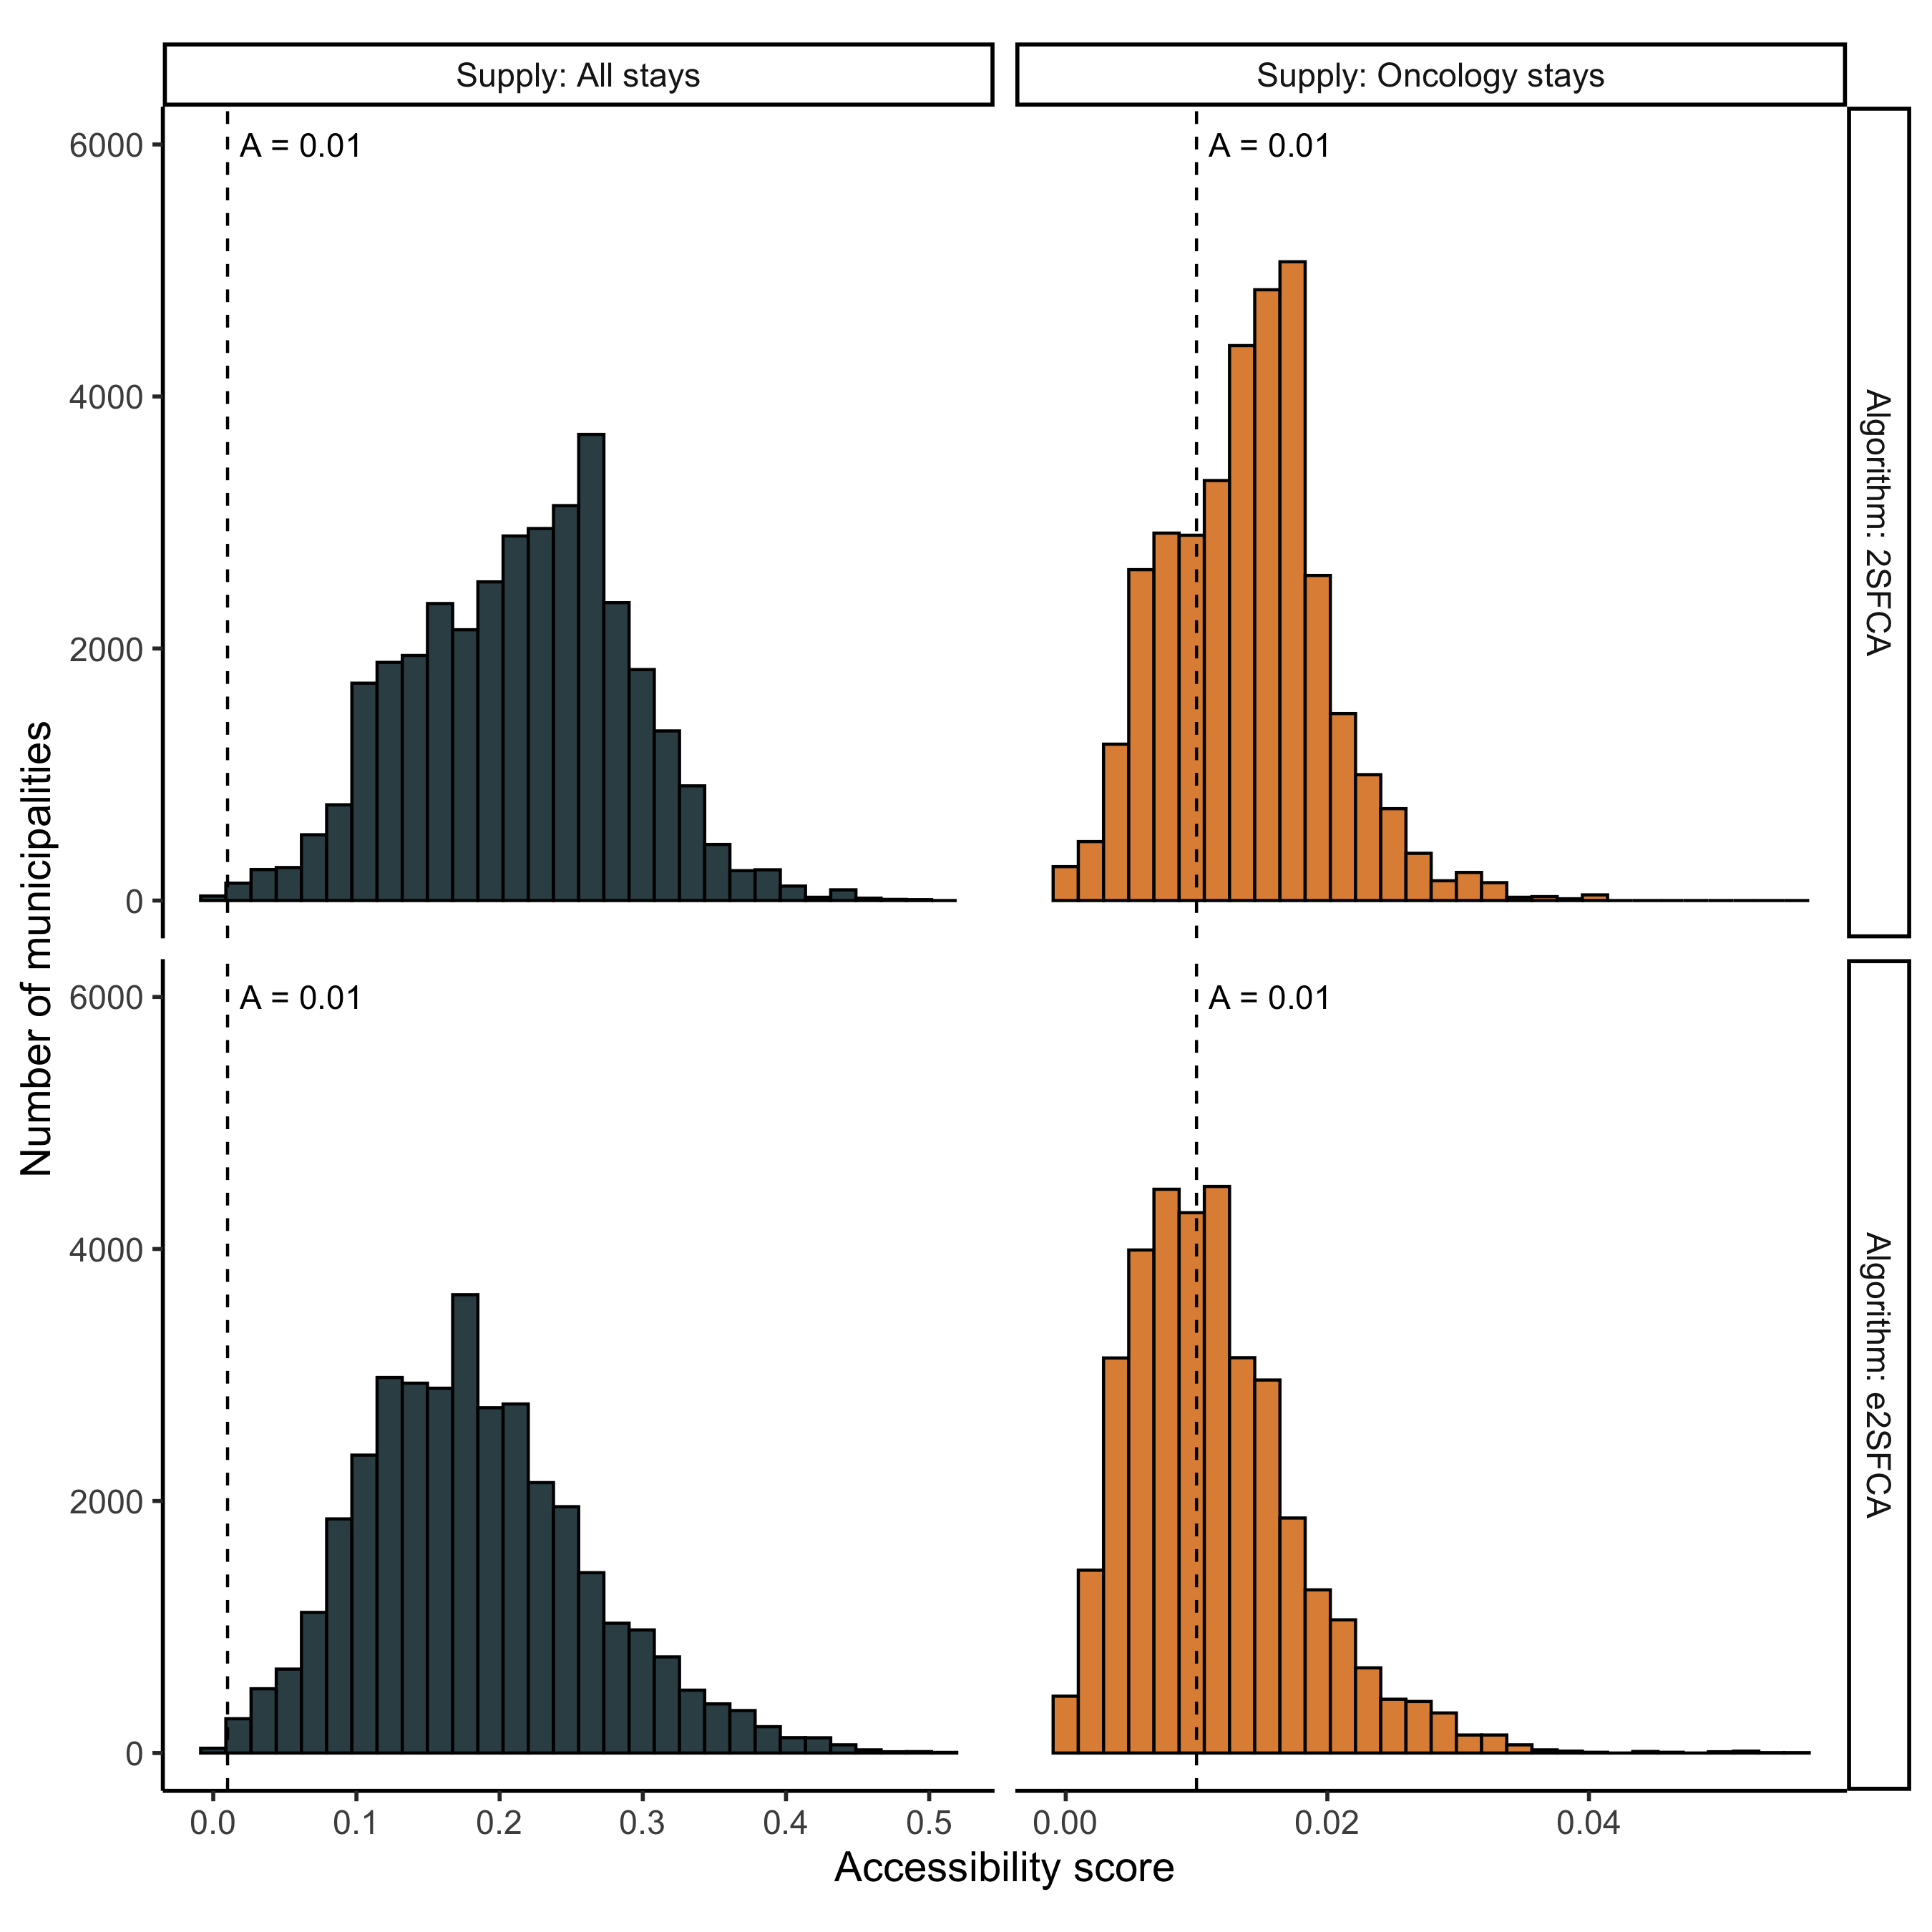
\includegraphics[width=0.7\textwidth]{images/camion/sup_fig5_accessibility_distribution.png}
    \centering
    \caption{ \textbf{Accessibility scores distribution.} The accessibility was
        lower with \ac{e2sfca} because of the weight decay. We also studied the
        influence of the supply variable in the accessibility score. Accessibility is
        much higher if we use the number of \ac{mco} stays as supply, instead of the
        oncology activity. This makes sense since oncology care centers are less common
        and the overall \ac{mco} activity is higher than the oncology activity. }
    \label{fig:accessibility-distribution}
\end{figure}

As we want to compute the accessibility to oncology care centers, we chose $S_u$
to be the oncology activity of a hospital $u$. We define oncology activity as
the sum of the number of medical and surgery stays related to cancer, and the
number of patients with chemotherapy or radiotherapy. A care center with no
oncology activity will have $R_u=0$ and a municipality that solely has access to
this care center u will have $A_i=0$. We use driving duration as travel
impedance metric, and we set the maximum catchment area to a 90-minute drive. In
2018, only 24,152 patients out of 761,057 (3.2\%) had travel duration greater
than 90 minutes for cancer related pathways. This is low enough to consider that
care centers are non-reachable beyond this distance. We divide the catchment
area into 3 intervals: $I_1=(0,30]$ ,$I_2=(30,60]$ and $I_3=(60,90]$. The
associated weights are respectively $W_1=1$, $W_2=0.042$ and $W_3=0.09$. These
sub catchment areas are set based on the cancer pathways travel duration
distributions and validated with medical experts. The weights are the same than
the \ac{e2sfca} paper \cite{luo_enhanced_2009}. For privacy reasons,
municipalities with small populations are grouped in entities called
``geographic codes'' in the \ac{pmsi} database. We decided to compute the
accessibility score for each geographic code and municipalities that are grouped
in the same code will have the same accessibility score.

\section{Results}

The oncology accessibility is unevenly distributed across the country, as
displayed on \cref{fig:accessibility-france}. For better readability, we cut the
accessibility scores into 5 quantiles. Q5 colored in dark green contains the top
20\% accessibility municipalities, and Q1 in light yellow contains the bottom
20\% ones. The lowest accessibility zones are mostly located in the center of
the country and in mountainous regions like the Alps or the Pyrenees. Plot (B)
shows that most of the population (51.6\%) lives in top 20\% accessibility
municipalities, while 6.3\% lives in the bottom 20\% quantile. On map (A), care
centers are displayed as squares, colored by cluster index, and sized by
oncology activity. We see that accessibility is highest near the most
specialized care centers. Indeed, the proportion of care centers from
specialized clusters decreases in lower accessibility quantiles (C). We then
ranked the departments by median accessibility and showed the top-10 and bottom
10 on plot (D). Among the top-5 departments, 4 are in Ile-de-France. Departments
from the bottom-10 are rural or mountainous areas like Lozère and
Alpes-de-Haute-Provence.  We notice disparities within departments as well, as
outlined by the large interquartile range in Hérault or Alpes-Maritimes. On the
contrary, this spread is very narrow in Ile-de-France departments.

\begin{figure}[h!]
    \includegraphics[width=0.9\textwidth]{images/camion/fig2_accessibility_france.png}
    \centering
    \caption{ \textbf{Distribution of the accessibility score computed with the
            \ac{e2sfca}, in metropolitan France.} Plot (A) shows municipalities
        colored by accessibility quantile. The care centers are drawn as
        squares, colored by cluster, and sized by oncology activity. Plot (B)
        shows the total population by accessibility quantile. Plot (C) displays
        the percentage of care centers by cluster by accessibility quantile.
        Plot (D) shows the top 10 and bottom 10 list of the departments, ranked
        by median accessibility. }
    \label{fig:accessibility-france}
\end{figure}

Accessibility score should be put into perspective with population density.
Overall, the denser municipalities have a median accessibility around 0.02.
Municipalities with low population densities have more extreme values.
\cref{fig:accessibility-vs-density} compares accessibility and population
density for three different regions: Provence-Alpes-Cote-d'Azur (A),
Ile-de-France (B), and Bourgogne-Franche-Comté (C). Municipalities are displayed
as squares, colored by accessibility quantile, and sized by population density.
These regions show very different profiles. In Provence-Alpes-Cote-d'Azur (A),
accessibility is essentially low in non-dense municipalities near the Alps.
However, in Bourgogne-Franche-Comté (C), we see dense municipalities with poor
accessibility scores, representing a large proportion of the region. We also
drew similar maps (D, E and F) where municipalities are colored based on the
average travel duration for patients with cancer in 2018. We see that the
average travel time is higher in municipalities with poor accessibility scores.

\begin{figure}[h!]
    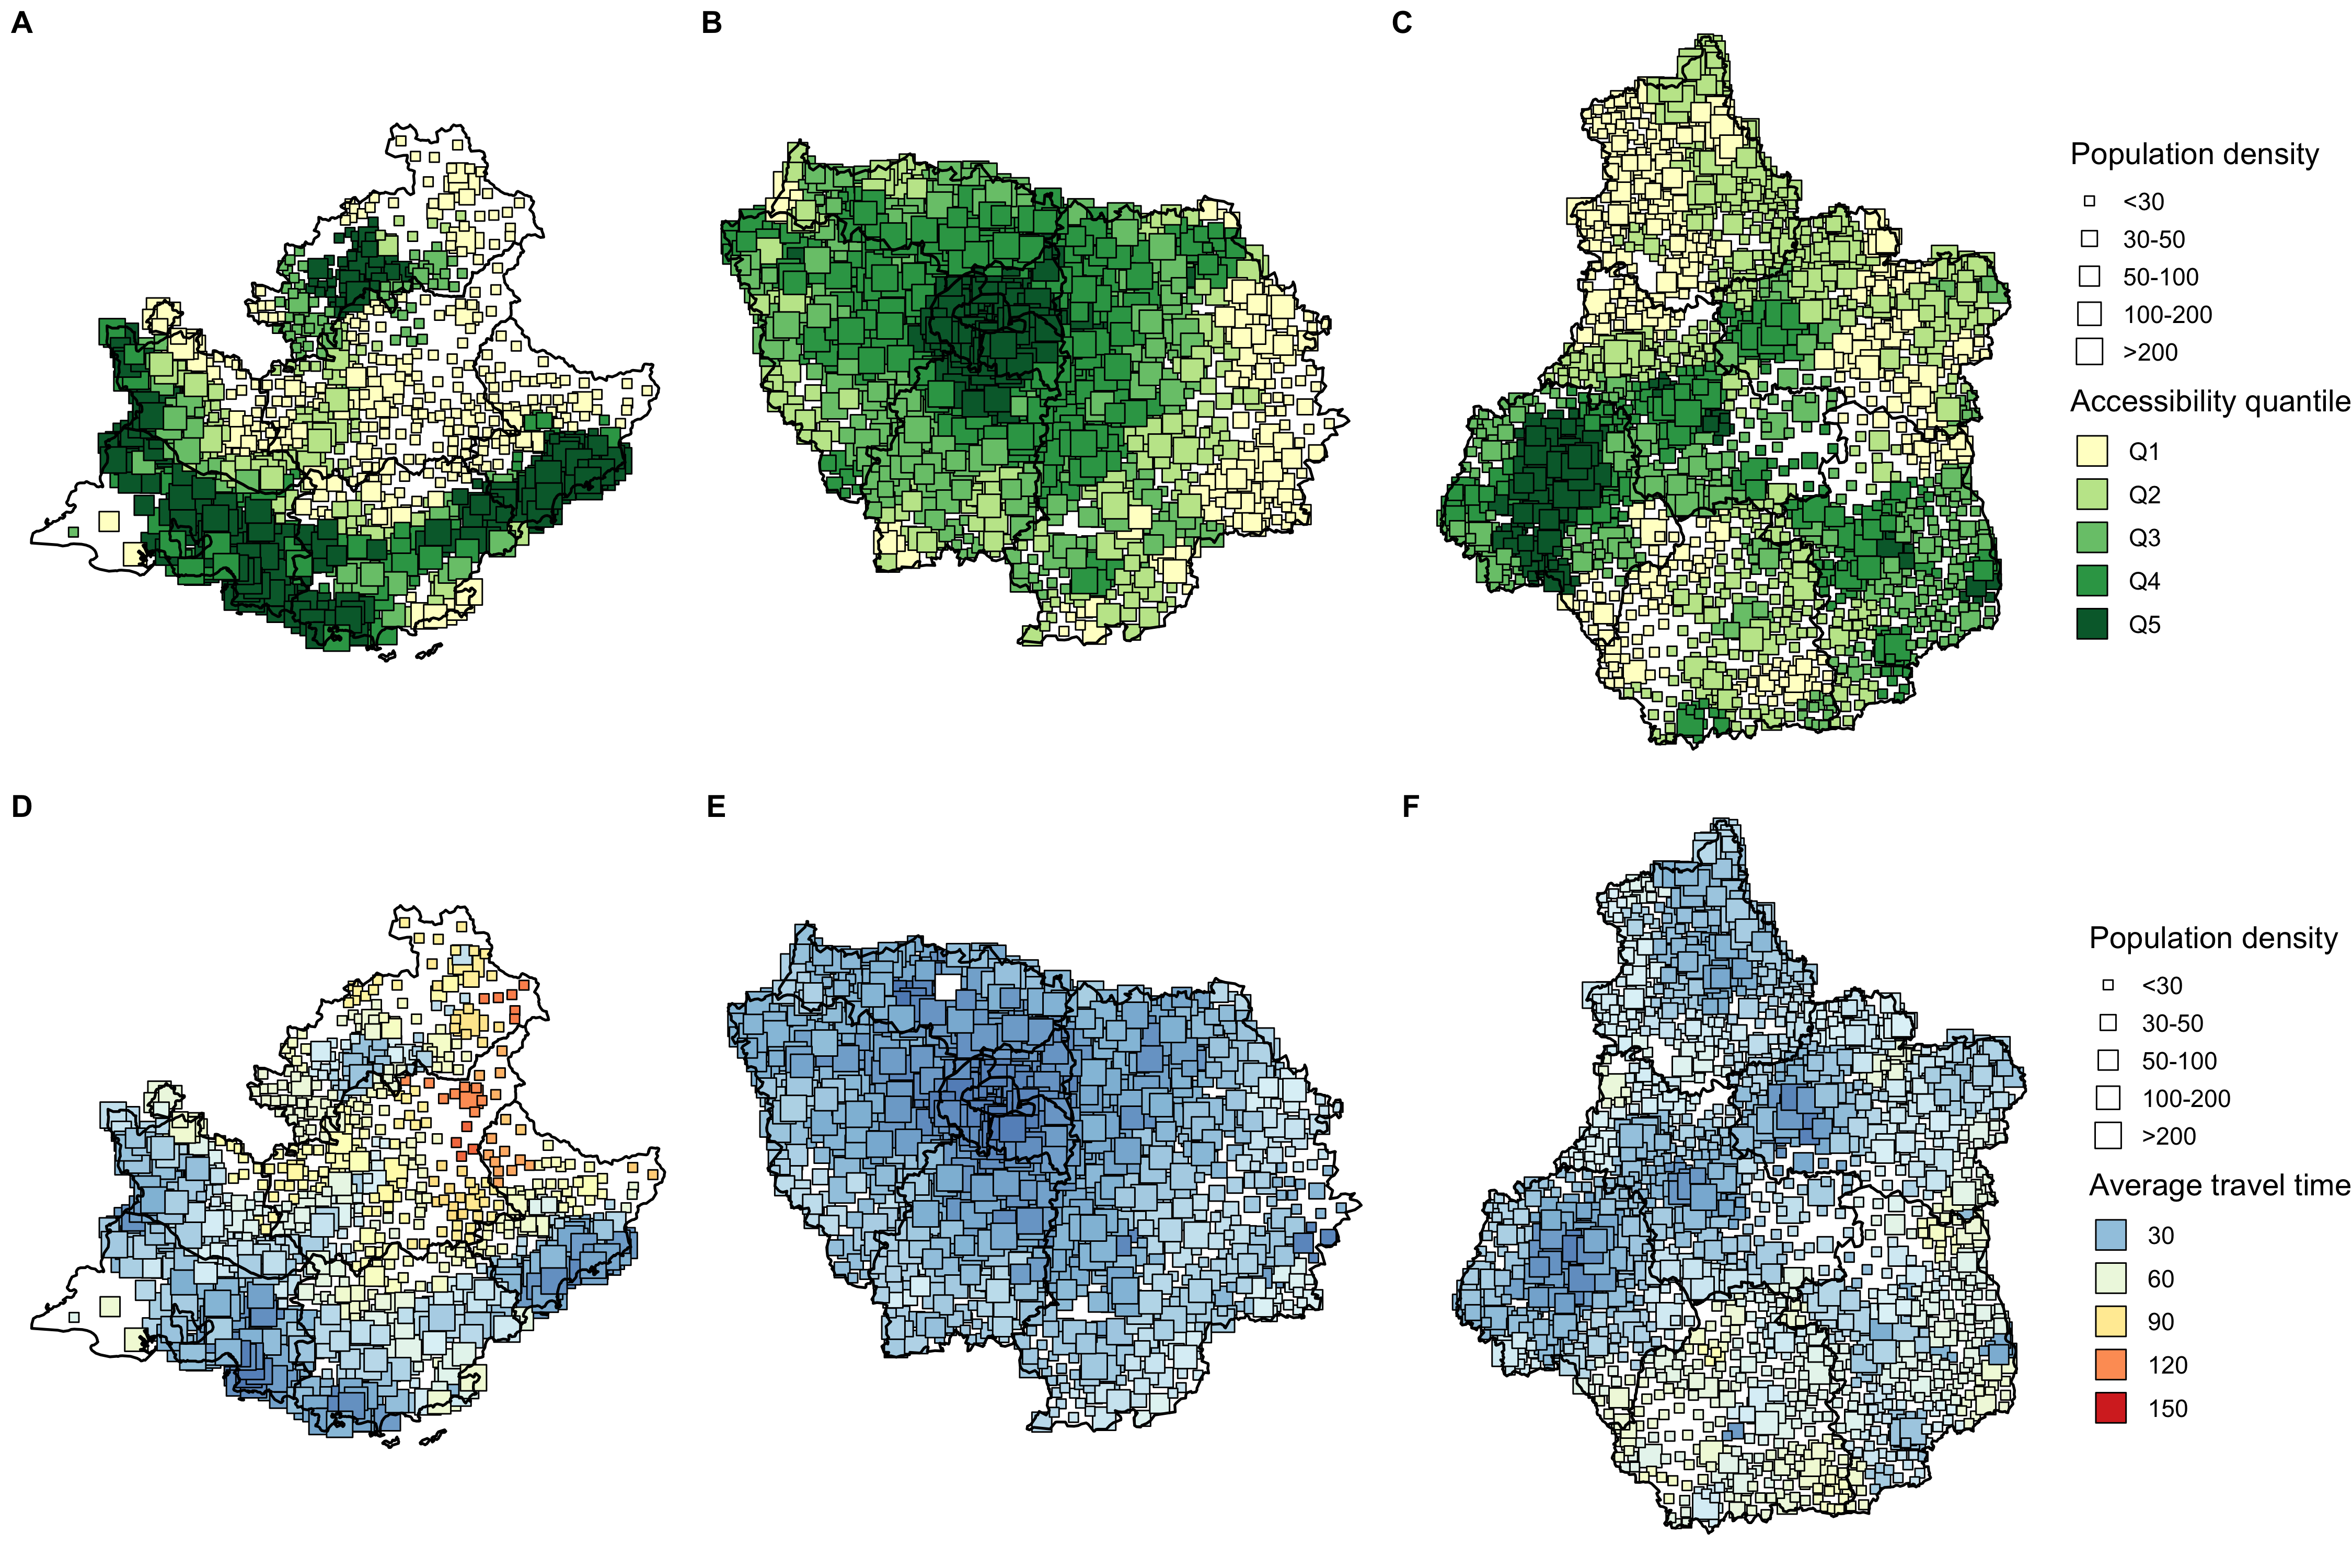
\includegraphics[width=0.9\textwidth]{images/camion/fig3_accessibility_vs_density_scatter_map.png}
    \centering
    \caption{ \textbf{Comparison of population density with accessibility scores
            and patient average travel time for cancer pathways.} Showing results in
        three regions: Provence-Alpes-Cote-d'Azur (A, D), Ile-de-France (B, E)
        and Bourgogne-Franche-Comté (C, F). Municipalities are drawn as squares,
        sized by population density and colored by either accessibility quantile
        (A, B, C) or patient average travel time (D, E, F). }
    \label{fig:accessibility-vs-density}
\end{figure}

Finally, we compared our accessibility score with the department exit ratio, by
municipality. Department exit ratio is defined as the proportion of cancer
patients who visited a care center outside from their department of residence
and was computed using the \ac{pmsi} database. In Provence-Alpes-Cote-d'Azur,
the exit ratio is higher in departments with low accessibility scores and few
oncology specialized care centers, as in Alpes-de-Haute-Provence and
Hautes-Alpes. While the Var department has some oncology centers, exit ratio
remains high since larger care centers are in Marseille and Nice.

\subsection{Accessibility distribution in metropolitan France regions}

\subsubsection{Accessibility in Provence-Alpes-Cote-d'Azur region}

We now focus on the region Provence-Alpes-Cote-d'Azur. This region is the far
southeastern on the mainland. The region's population was 5,048 million in 2018.
Its prefecture and largest city is Marseille. The region contains six
departments. Bouches-du-Rhone, Var and Alpes-Maritimes are located on the
coastline and gather the largest cities like Marseille, Nice, or Toulon.
Alpes-de-Haute-Provence, Vaucluse, and Hautes-Alpes are inland departments, with
a majority of rural and mountainous areas. Results are shown on
\cref{fig:accessibility-paca}. By comparing maps (A) and (B), we confirm that
the accessibility is maximum in denser areas of the region. Average patients
travel time are displayed on map (C) and we drew the major roads (primary,
motorway and truck) in red. The road system is well developed on the coast,
rallying the larger cities of the region. However, driving from the rural areas
in the Alps to the major cities is hard, resulting in higher travel times. The
accessibility is unevenly spread within the departments, especially in
Alpes-Maritimes where the distribution is multi-modal (D). There, cities like
Nice and Cannes have large hospitals thus good accessibility, while the northern
areas of the department are mostly mountains. Accessibility is higher in
municipalities with dense populations, for all the departments (E). Finally, the
average travel time decreases when the accessibility score increases. This makes
sense since the accessibility score was computed based on the driving distance
between population locations and care centers. However, it confirms that
patients living in poor accessibility zones effectively travel further to seek
oncology care. In Bouches-du-Rhone, nearly all the municipalities have an
average travel time lower than 30 minutes, while in Alpes-de-Haute-Provence,
average travel times are rarely lower than 60 minutes (F).

\begin{figure}[h!]
    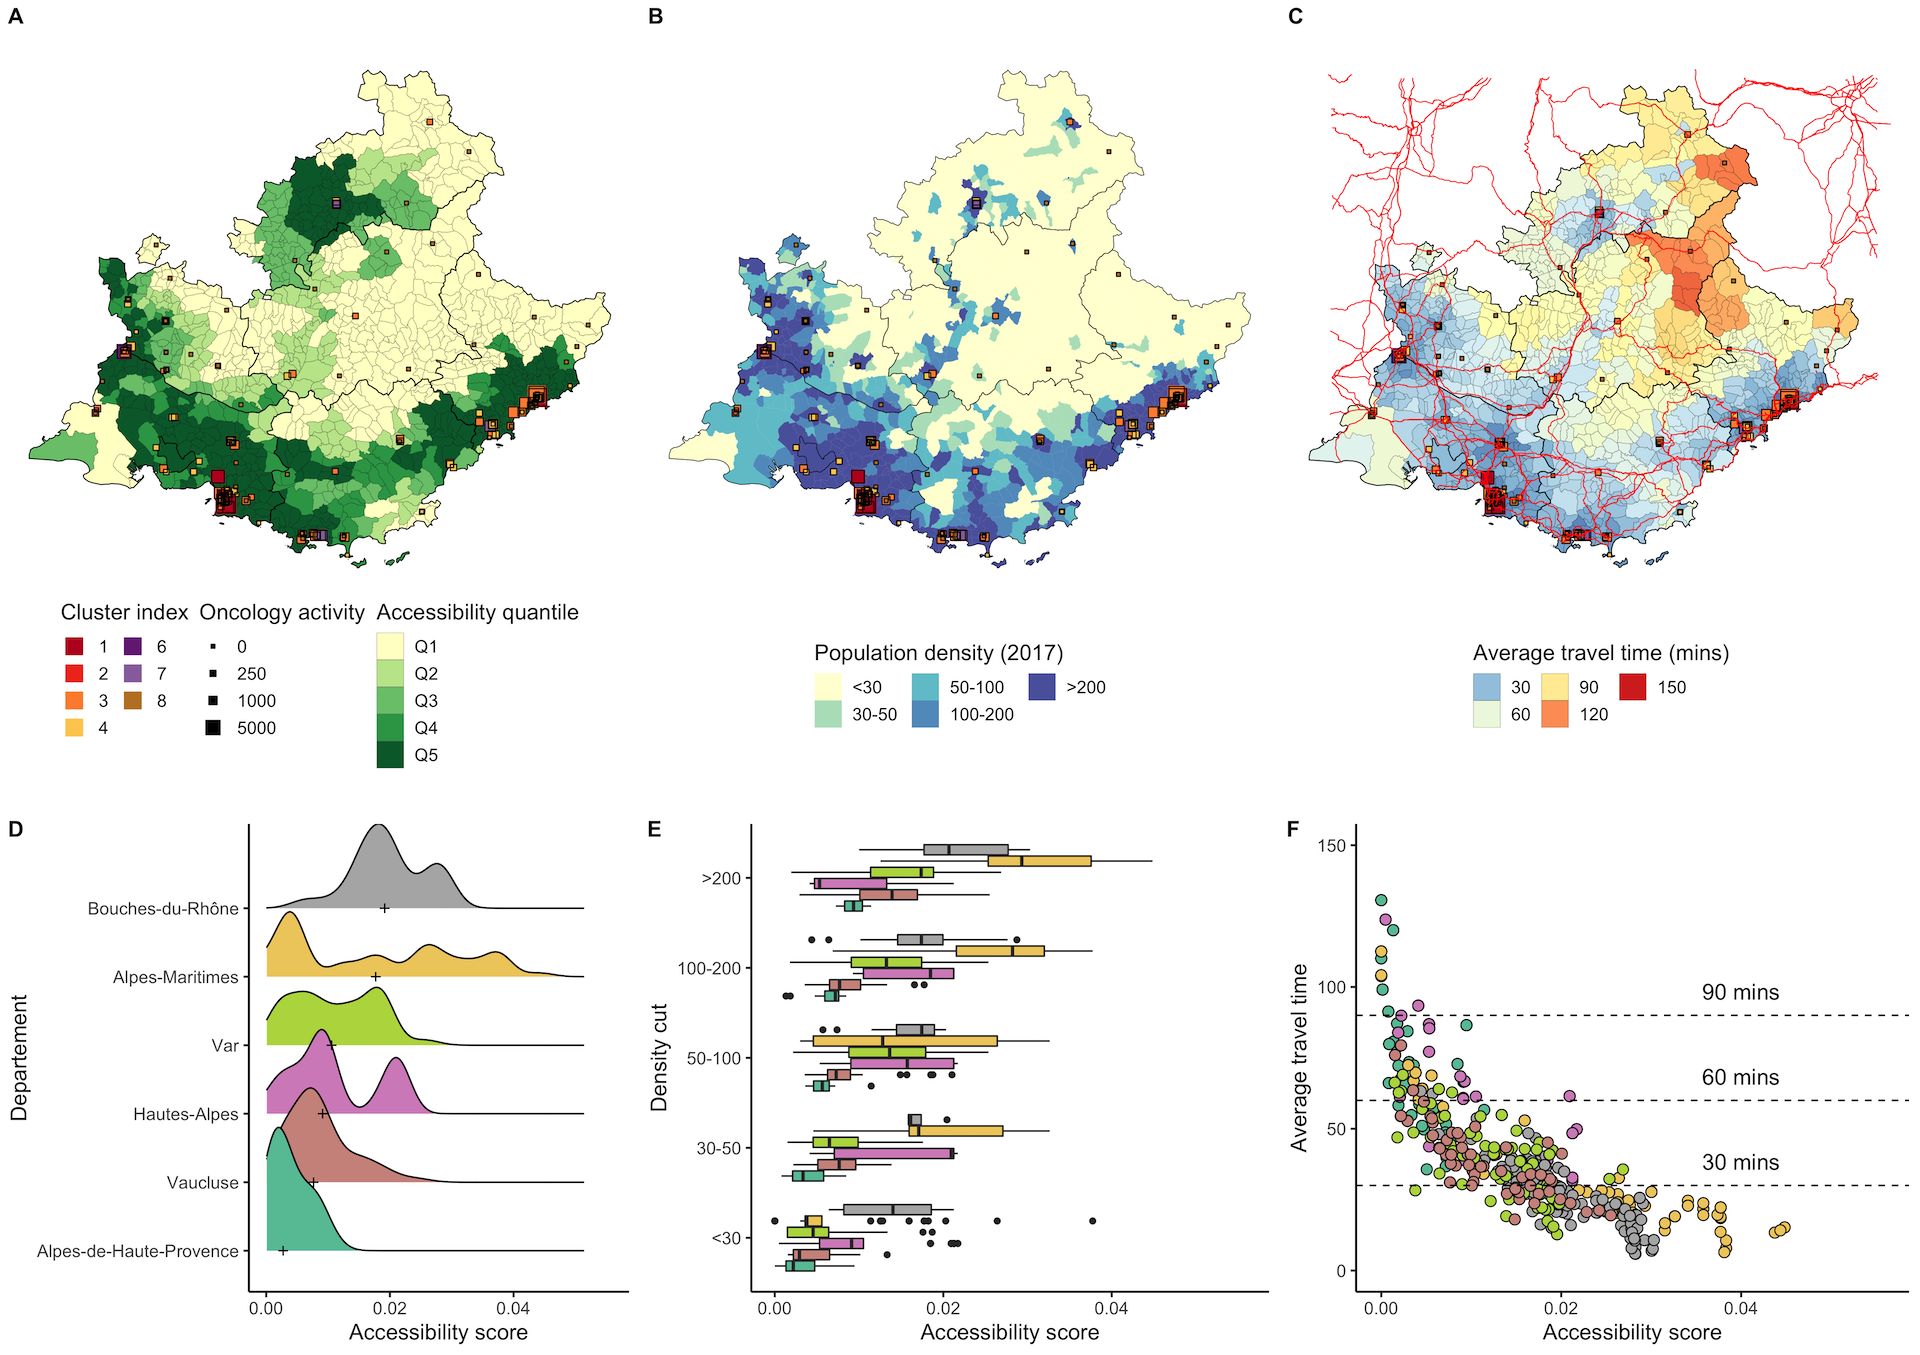
\includegraphics[width=0.9\textwidth]{images/camion/fig4_accessibility_Provence-Alpes-Cote-d'Azur.png}
    \centering
    \caption{ \textbf{Accessibility distribution in Provence-Alpes-Cote-d'Azur
            region.} Map (A) shows the region accessibility distribution per
        municipality. Map (B) displays the population density discretized in 5
        bins. The map on plot (C) displays the average travel time for cancer
        pathways. Large roads (primary, motorway and trucks) are drawn in red.
        Plot (D) shows the accessibility distribution per department of the
        region. Plot (E) shows the accessibility distribution by municipality
        population density and department. Plot (F) compares the accessibility
        score from municipalities with the average travel time for cancer
        pathways. }
    \label{fig:accessibility-paca}
\end{figure}

\subsubsection{Accessibility in Pays de la Loire region}

The Pays de La Loire region is located in the west of France. It covers 32,082
km\textsuperscript{2} which makes it the largest region in France, with a
population of 3,806,461 (Insee) in 2019. In the region, one out of two
inhabitants lives in rural areas, compared to one out of three on average in
France. The Pays de la Loire is thus the 4th most rural region behind New
Aquitaine, Brittany and Burgundy-Franche-Comté.  The Pays de La Loire region is
composed of 5 departments. The level of population living in rural communes
varies according to the departments, but 4 departments out of the 5 are
considered rural.  In Vendée and Mayenne, two out of three inhabitants live in
rural areas, in Maine-et-Loire 58\% of the population resides in a rural commune
and in Sarthe 56\%. However, 29\% of the region's population lives in a rural
commune under the influence of a pole, compared to 20\% in an independent rural
commune. The city of Nantes, located in Loire-Atlantique in the east of the
region, is the largest urban area in the region and has 303,382 inhabitants, as
well as 961,521 inhabitants in its urban unit. The region has several cities
with more than 100,000 inhabitants with Le Mans and its 143,325 inhabitants,
Angers (151,520 inhabitants), followed by cities of about 50,000 inhabitants
such as Saint-Nazaire, (68,200 inhabitants) Cholet, (54,200 inhabitants) and
Laval (51,000 inhabitants). The Pays de la Loire has good accessibility with
51\% of its population living in a territory with maximum accessibility and a
low rate of its population living in territories with low or very low
accessibility: 8.3\% of its population resides in an accessibility score zone of
Q2 and only 3.7\% of its population in Q1. Thus, the maps show a good
distribution of accessibility across the territory that varies proportionally
with population density, with low accessibility areas corresponding to areas
with low or very low population density. Travel time is also relatively evenly
distributed across the region, with average travel times of 30 minutes, although
depending on the department, a significant proportion of trips are between 30
and 60 minutes. A very small proportion of territories exceed 60 minutes of
travel time. The territories with longer travel times are located in the Vendée
department, mainly due to the coastal profile of the department and the islands
that make it up, such as the Noirmoutier peninsula or the Ile d'Yeu, where
travel times exceed 90 minutes and 120 minutes respectively.

\begin{figure}[h!]
    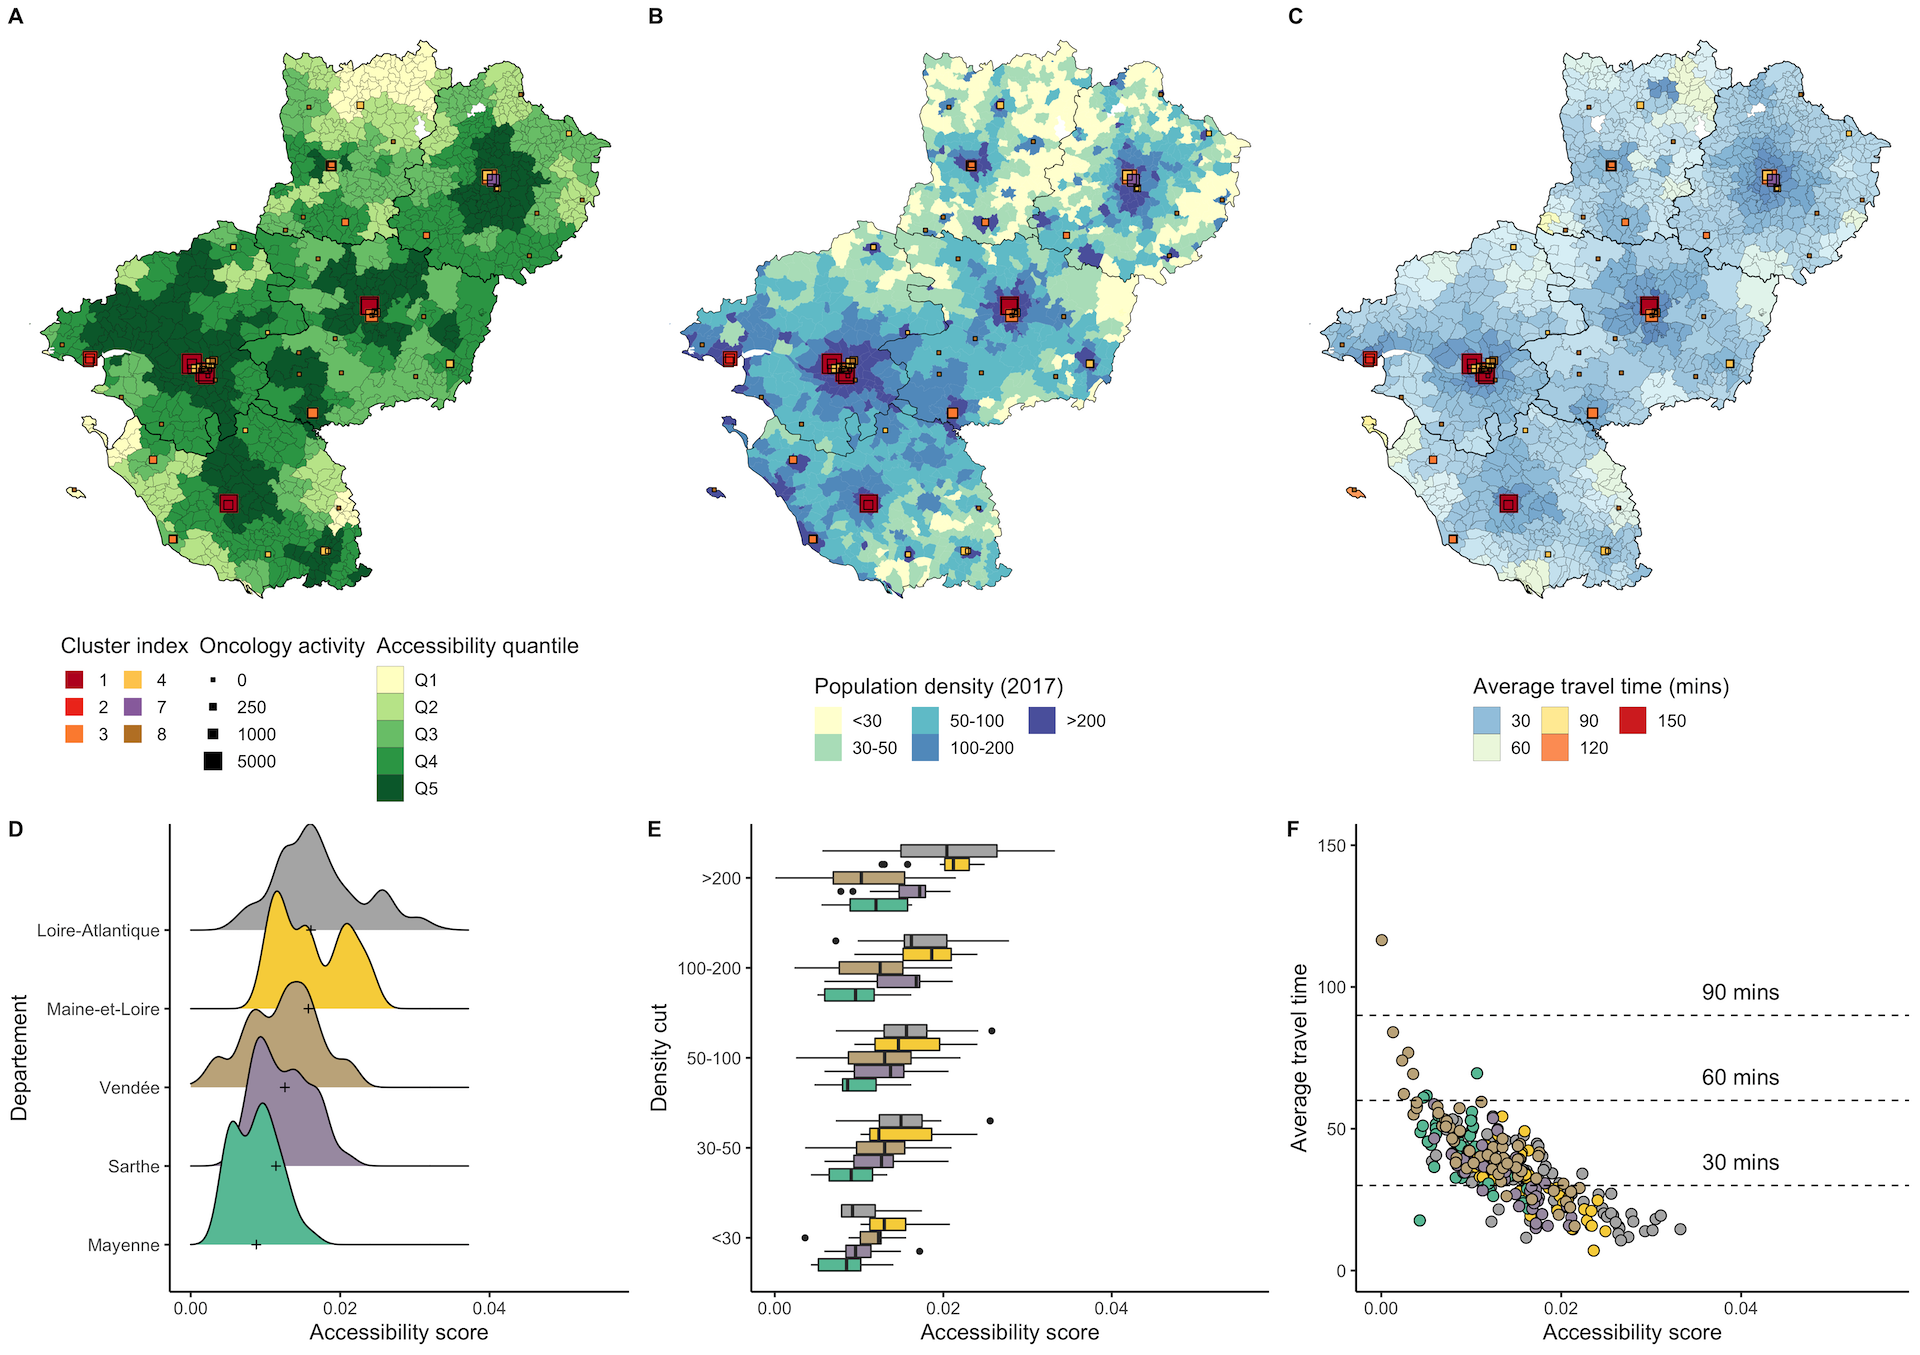
\includegraphics[width=0.9\textwidth]{images/camion/region_accessibility/accessibility_Pays-de-la-Loire.png}
    \centering
    \caption{
        \textbf{Accessibility distribution in Pays-de-la-Loire.} The accessibility distribution
        in this region is high, and the amount of municipalities with Q5 accessibility
        score is very low. The median accessibility is the highest in Loire-Atlantique
        department, especially around Nantes; or in Maine-et-Loire near Angers. The
        lowest median accessibility is in Mayenne, where the main city is Laval. The
        accessibility is lower in the northern part of this department, where the
        population density decreases compared to the rest of the region.
    }
\end{figure}

\subsubsection{Accessibility in Occitanie region}

The Occitanie region is located in the South of France. It covers 72,724 km² for
a population of 5,933,185 (Insee) in 2019, for a population density of 81.6
inhabitants/km² the 6th least dense region in metropolitan France. The rural
territory in Occitanie represents 90\% of the territory, mainly present in the
mountain areas of the Massif Central and Pyrenees. The urban space is mainly
found along the coast and in the Garonne basin. 39\% of the population lives in
rural areas, i.e. 2.9 million inhabitants, and 9 of the 13 departments are
considered rural. However, Occitanie is a largely urbanized territory with
numerous urban centers in each department, the main metropolises being Toulouse
and Montpellier. This region is the 5th most urbanized region of the metropolis
and has more than fifty urban units of at least 10,000 inhabitants with several
cities exceeding 70,000 inhabitants (Tarbes, Montauban, Albi). 4.4 million
people live in the urban units, representing 76\% of the population. Occitanie
is composed of 13 departments. Three departments are among the most urbanized in
the province and therefore have a strong demographic weight: Hérault (89\% of
the population residing in an urban unit), Pyrénées-Orientales (88\%) and
Haute-Garonne (87\%). The Hérault department includes the city of Montpellier,
but also Béziers, Sète and many small urban areas. The Haute Garonne includes
the city of Toulouse, the fourth most populated commune in France (493,465
inhabitants) and with its rural areas are under strong pole influence.  The Lot,
Lozère and Gers are the least urbanized in France, with less than 40\% of the
population living in urban areas.

In this region, accessibility is not uniform across the territory. The areas
with the highest accessibility scores are concentrated in the large urban areas
and their catchment areas, notably in the center of the region around the city
of Toulouse and Montauban in the Garonne basin, as well as along the coastline
in the east of the region around the cities of Nîmes, Montpellier, Béziers,
Narbonne and Perpignan. Also, if the most densely populated areas have a good
level of accessibility, it can be seen that some medium-sized cities in the
Occitanie region lack a good level of accessibility and even have low
accessibility. This is particularly pronounced in the rural departments of the
region (Lot, Gers and Lozère), as well as in Aude, Ariège and Hautes-Pyrénées.
Indeed, many urban units have a low accessibility score (Q2) such as Auch
(25,527 inhabitants) in the Gers, Foix (12,310 inhabitants) and Pamiers (29,340
inhabitants) in the Ariège, Rodez (47,868 inhabitants) in the Aveyron with a
score of Q2/Q3, Cahors (24,279 inhabitants) in the Lot. Many areas of the region
have long travel times of around 90 minutes if not 120 minutes on average. This
is particularly true along the border with Spain, which is characterized by its
mountainous terrain. However, the Gers, Lot, Lozère, Aveyron and Hérault regions
have average travel times of around 90 minutes. These high travel times are
mainly associated with sparsely populated areas, although in the Hautes-Pyrénées
department, average travel times of 90 minutes can be seen around the urban unit
of Bagnères de Bigorre (13,213).

\begin{figure}[h!]
    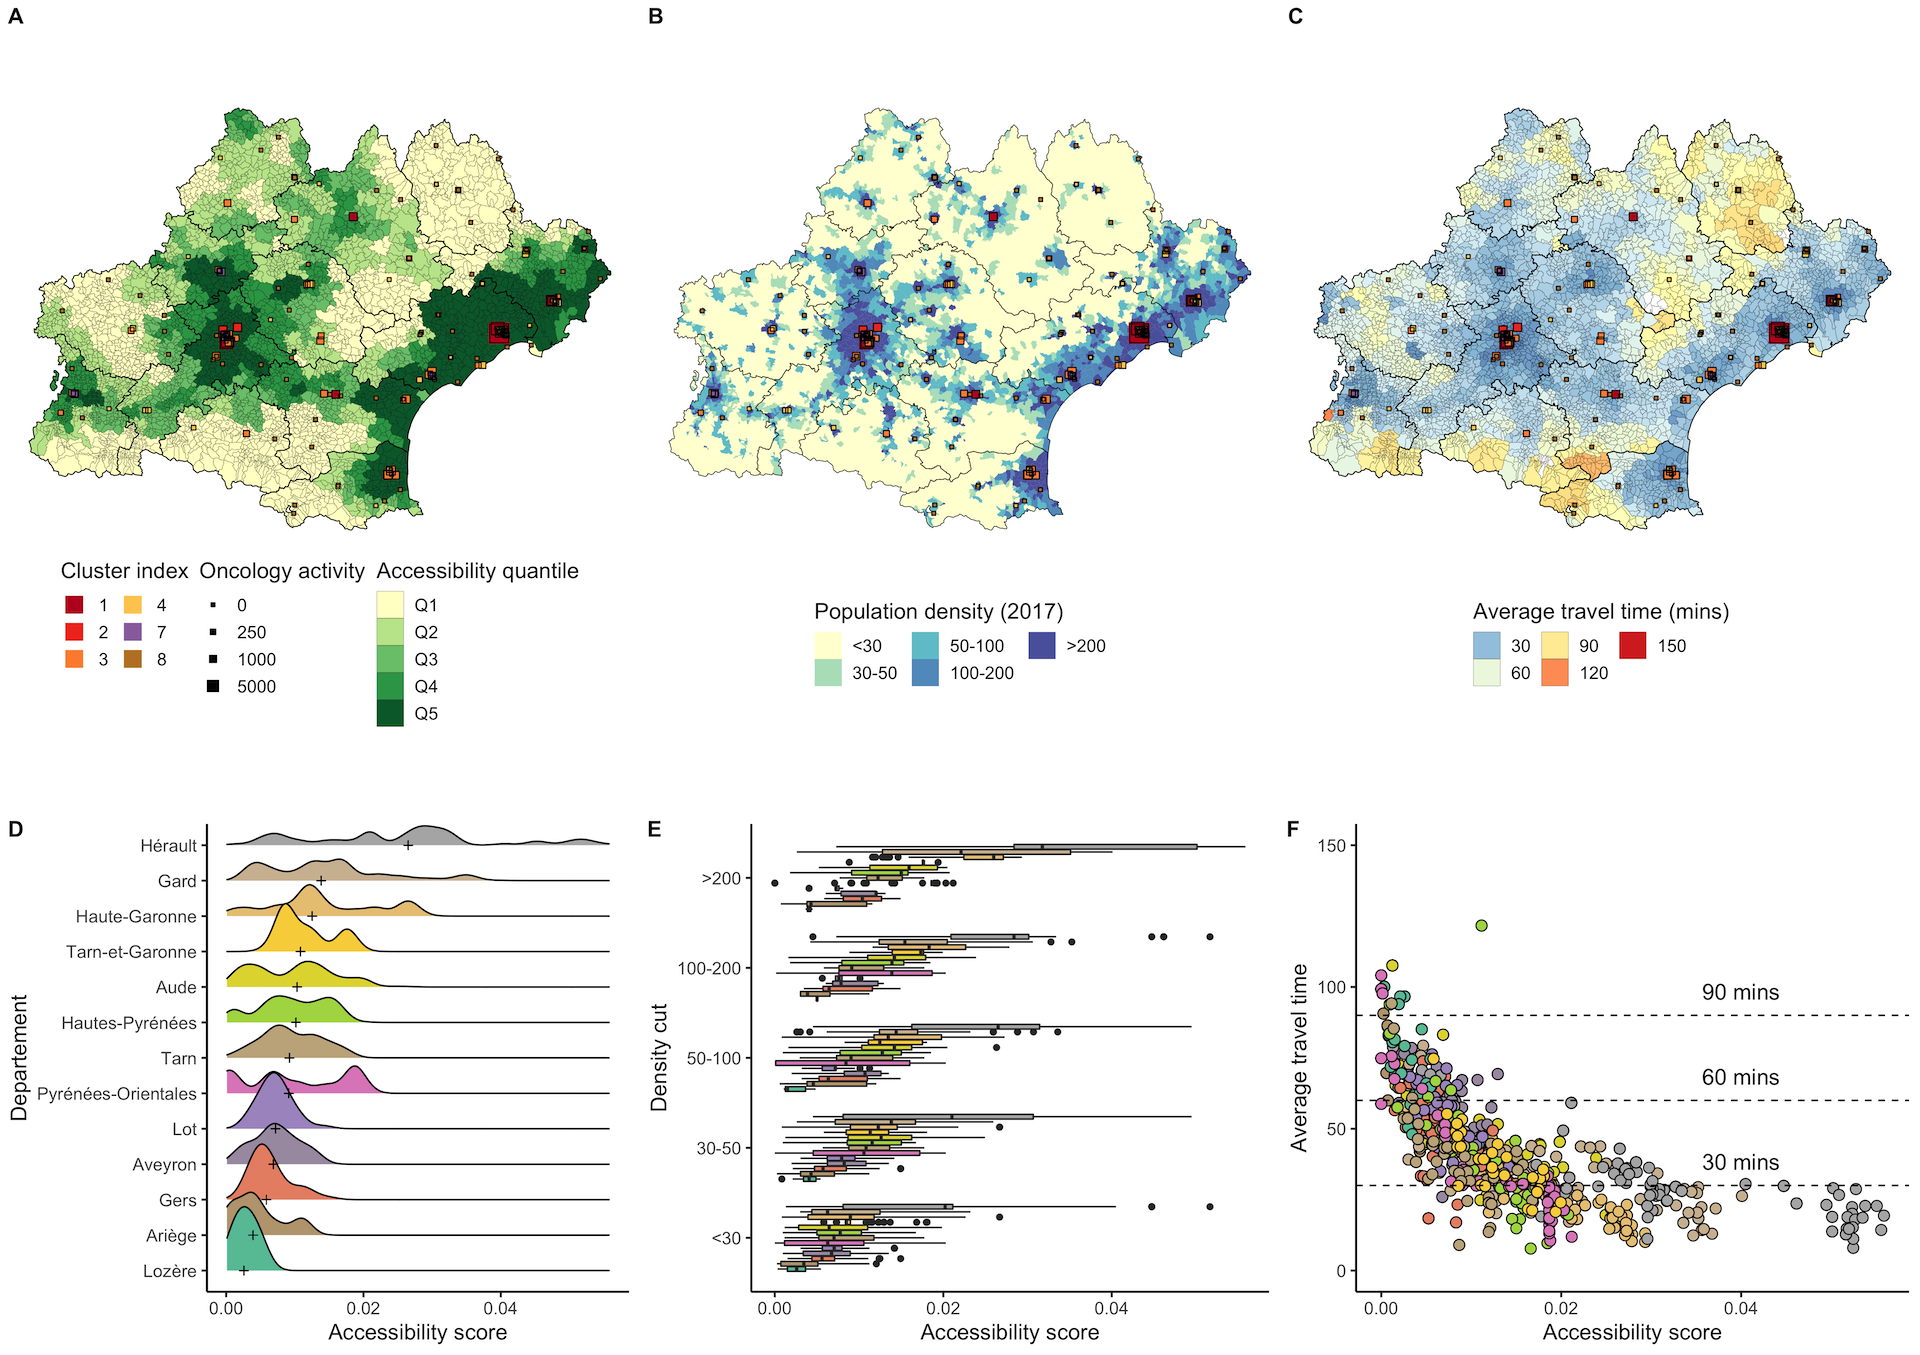
\includegraphics[width=0.9\textwidth]{images/camion/region_accessibility/accessibility_Occitanie.png}
    \centering
    \caption{
        \textbf{Accessibility distribution in Occitanie.} The areas with the highest accessibility scores are concentrated in
        the large urban areas and their catchment areas, notably in the center of the
        region around the city of Toulouse and Montauban in the Garonne basin, as well
        as along the coastline in the east of the region around the cities of Nîmes,
        Montpellier, Béziers, Narbonne and Perpignan.
    }
\end{figure}

\subsubsection{Accessibility in Nouvelle-Aquitaine region}

The Nouvelle-Aquitaine region is located in the southwest of France. It covers
an area of 84,036 km\textsuperscript{2} which makes it the largest region in
France, with a population of 6,010,289 (Insee) in 2019. The region is the third
most rural region of France with half of its inhabitants living in a rural
commune. The share of population in rural autonomous is significant compared to
the national average but is similar to that of Brittany or
Burgundy-Franche-Comté. Among the twelve departments of Nouvelle-Aquitaine , ten
are predominantly rural, and two are predominantly urban: Gironde (71\% of the
population living in an urban commune) and Pyrénées-Atlantiques (62\%).
Nouvelle-Aquitaine is composed of 12 departments. The region's main metropolis,
Bordeaux, with 260,958 inhabitants and 986,879 inhabitants in its urban unit, is
located in the west of the region in the Gironde department. The region includes
several intermediate cities with more than 70,000 inhabitants such as Limoges
(130,876), Poitiers (89,212), Pau (75,627), La Rochelle (77,205), Mérignac
(72,197), Pessac (65,245).

We notice accessibility disparities in this region. The areas with the highest
accessibility scores are mainly located around the above-mentioned large and
intermediate cities. Also, the areas with accessibility scores Q1 and Q2 are
mainly located in territories with low or very low population density.
Similarly, the Nouvelle-Aquitaine region seems to provide relatively widespread
access to cancer care for its population. Indeed, 56\% of its population is
located in a zone with a maximum accessibility score of Q5, and 21.1\% in a zone
with a very good accessibility score of Q4. This leaves a smaller share of the
population in areas of low accessibility (8.4\% in Q2) and very low
accessibility (6.3\% in Q1). The average travel time is well distributed over
the territory, with a majority of the territory covered by travel times between
30 and 60 minutes. It can be seen, however, that part of the territory has a
good share of trips of less than 30 minutes (on average e 15 minutes) even in
areas with average accessibility (score 0.2). A clear correlation can be seen
between accessibility score and average travel time, with longer travel times in
areas with low accessibility scores, but consequently less densely populated
territories. The Landes and Lot-et-Garonne are the departments with the highest
number of trips exceeding 60 minutes.

\begin{figure}[h!]
    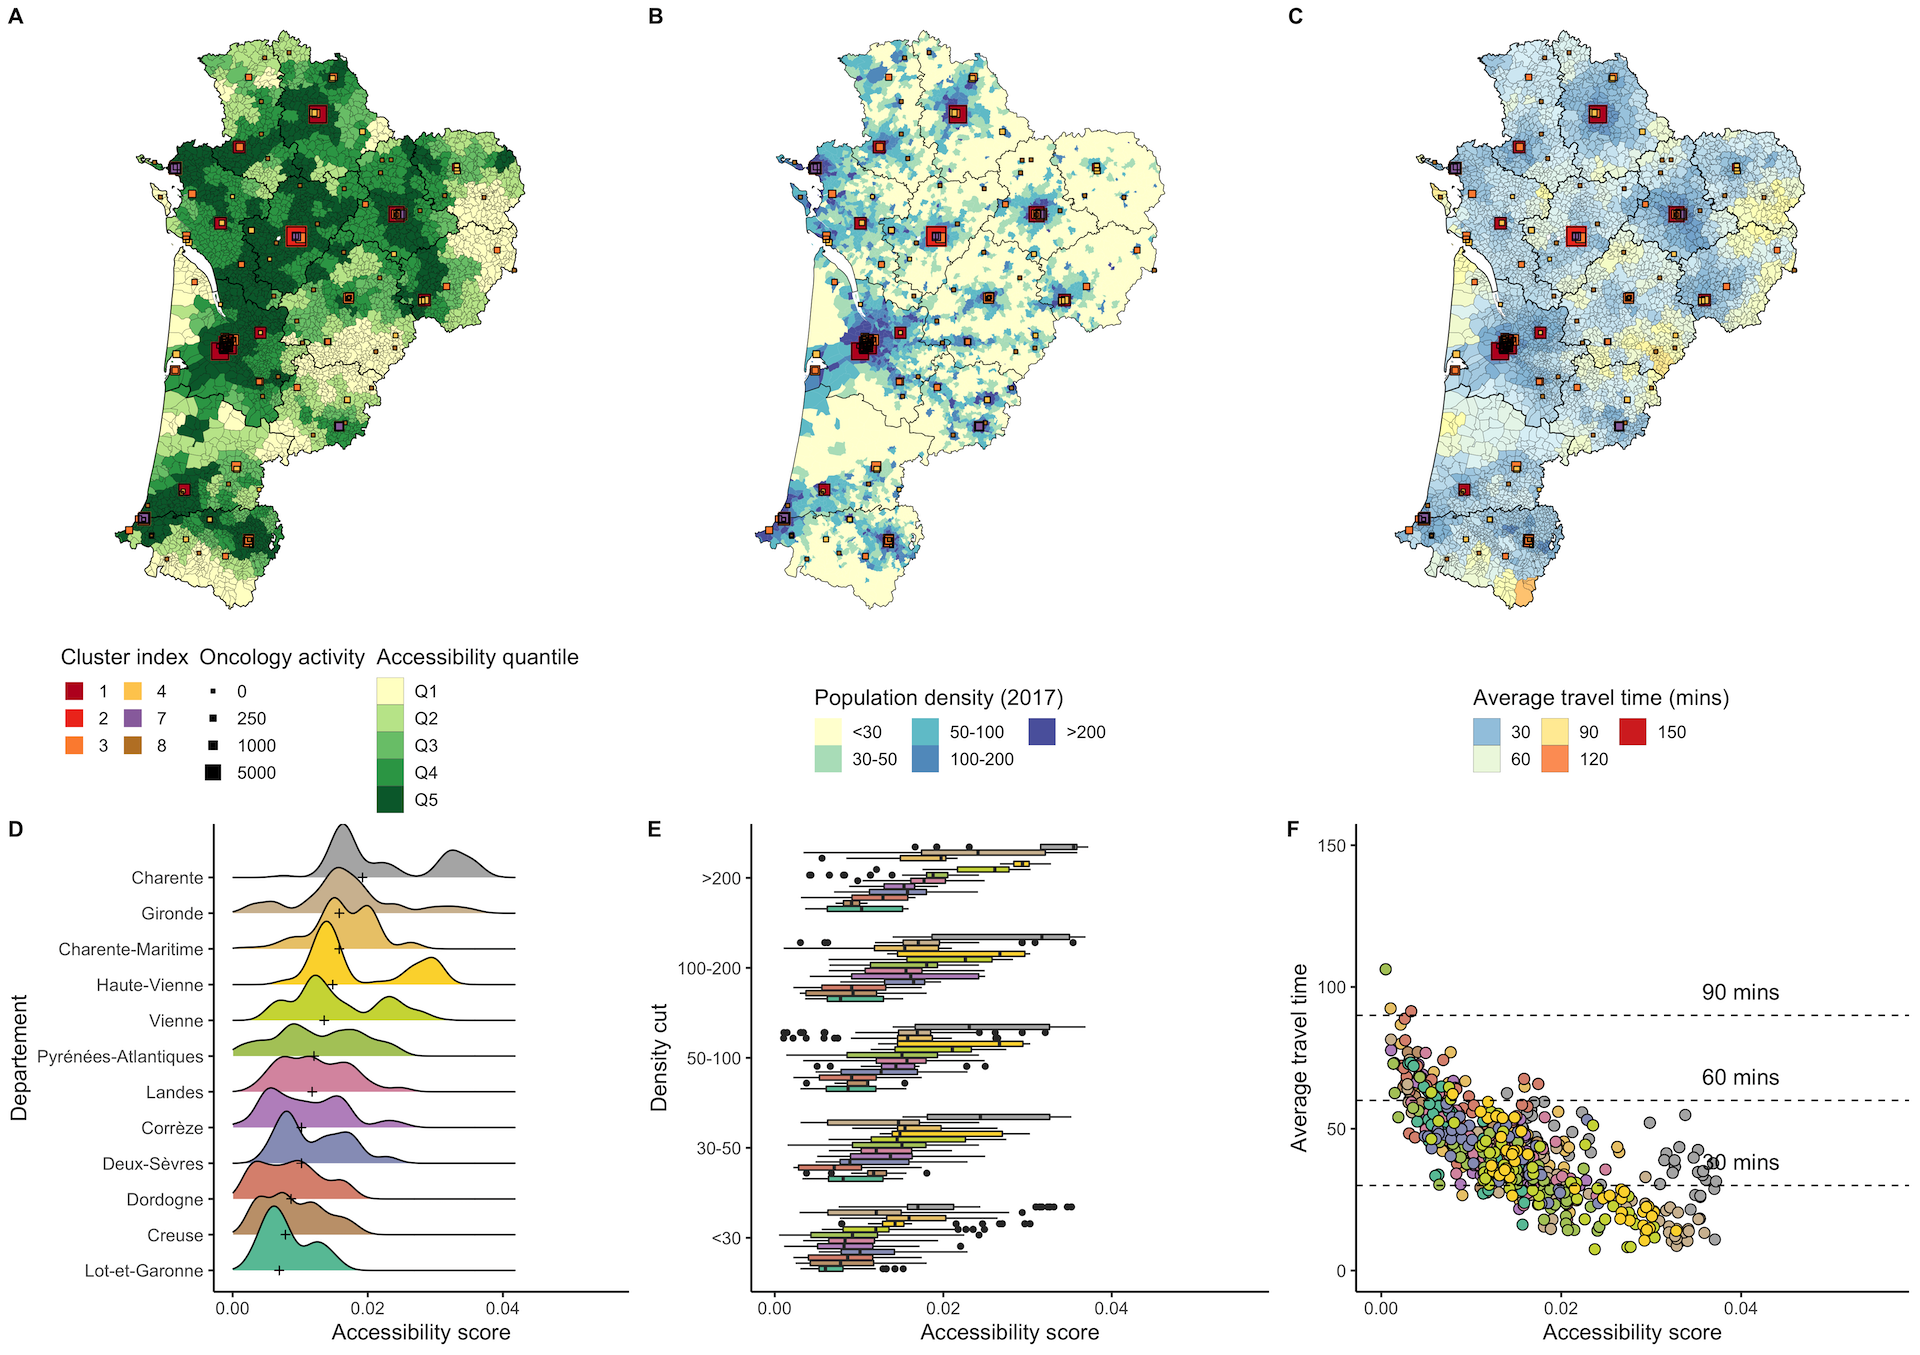
\includegraphics[width=0.9\textwidth]{images/camion/region_accessibility/accessibility_Nouvelle-Aquitaine.png}
    \centering
    \caption{
        \textbf{Accessibility distribution in Nouvelle-Aquitaine.}The areas with the highest accessibility scores are mainly located around the
        above-mentioned large and intermediate cities. Also, the areas with
        accessibility scores Q1 and Q2 are mainly located in territories with low or
        very low population density. The Nouvelle-Aquitaine region seems to
        provide relatively widespread access to cancer care for its population.
    }
\end{figure}

\subsubsection{Accessibility in Normandie region}

The Normandie region is located in the north-east of France. It covers 29,905
km² with a population of 3,325,032 inhabitants (Insee) in 2019. The Normandie
region remains a fairly rural region with half of its inhabitants living in a
rural commune (49\% compared to 40\% in the rest of France). The population
living in a rural commune is clearly in the majority in Orne in the south of the
region (73\%), Manche in the west (68\%) and Eure in the east (62\%). However,
more than half of the rural communes are not under the influence of a hub.
Normandie is composed of 5 departments. The department of Seine-Maritime in the
northeast of the region has two of the largest urban units in the region with
more than 200,000 inhabitants: Rouen the most populous with 112,321 inhabitants
and 471,893 in its urban unit as well as Le Havre with 172,366 inhabitants and
233,414 in its urban unit. The third urban unit of more than 200,000 inhabitants
in the region is Caen with 206,973 inhabitants in its urban unit, located in
Calvados. Normandie presents a rather average accessibility in terms of
population density and accessibility ratio since 30.9\% of its population lives
in the best accessibility score almost equivalent to the percentage of
population living in a territory with a Q3 score of 28.3\%. Only 10.3\% of its
population lives in accessibility level Q1 and 9.2\% in Q2.


We notice that the accessibility score is unevenly distributed. Although the
areas with low or very low population density are the most affected by a low
accessibility score of Q1 or Q2, we can still observe a fairly homogeneous
distribution of the population on the territory, especially in the areas far
from the urban units, and an accessibility that remains fairly low around Q2.
The department of Calvados has the best distribution of accessibility over its
entire surface. Whereas Orne, which is the most rural department in Normandie,
has an accessibility score of Q1 except around the urban unit of Argentant. The
same is true for the department of La Manche, which includes many areas of the
territory with an accessibility score of Q1 or especially Q2 despite a higher
population density, notably around the city of Cherbourg-Octeville and its
surroundings with an accessibility score of Q3 or even Q2 for a city that
nevertheless counts 35,545 and 81,423 in its urban unit (Figure 24). The average
travel time is well distributed over the territory, with the majority of the
territory covered by travel times of 30 minutes on average and below 60 minutes.
It can be seen that the majority of trips in the departments of Seine-Maritime
and Calvados are under 30 minutes, particularly in Calvados, unlike the
department of Orne, the only department in the region whose trips are slightly
over 60 minutes but still under 90 minutes.

\begin{figure}[h!]
    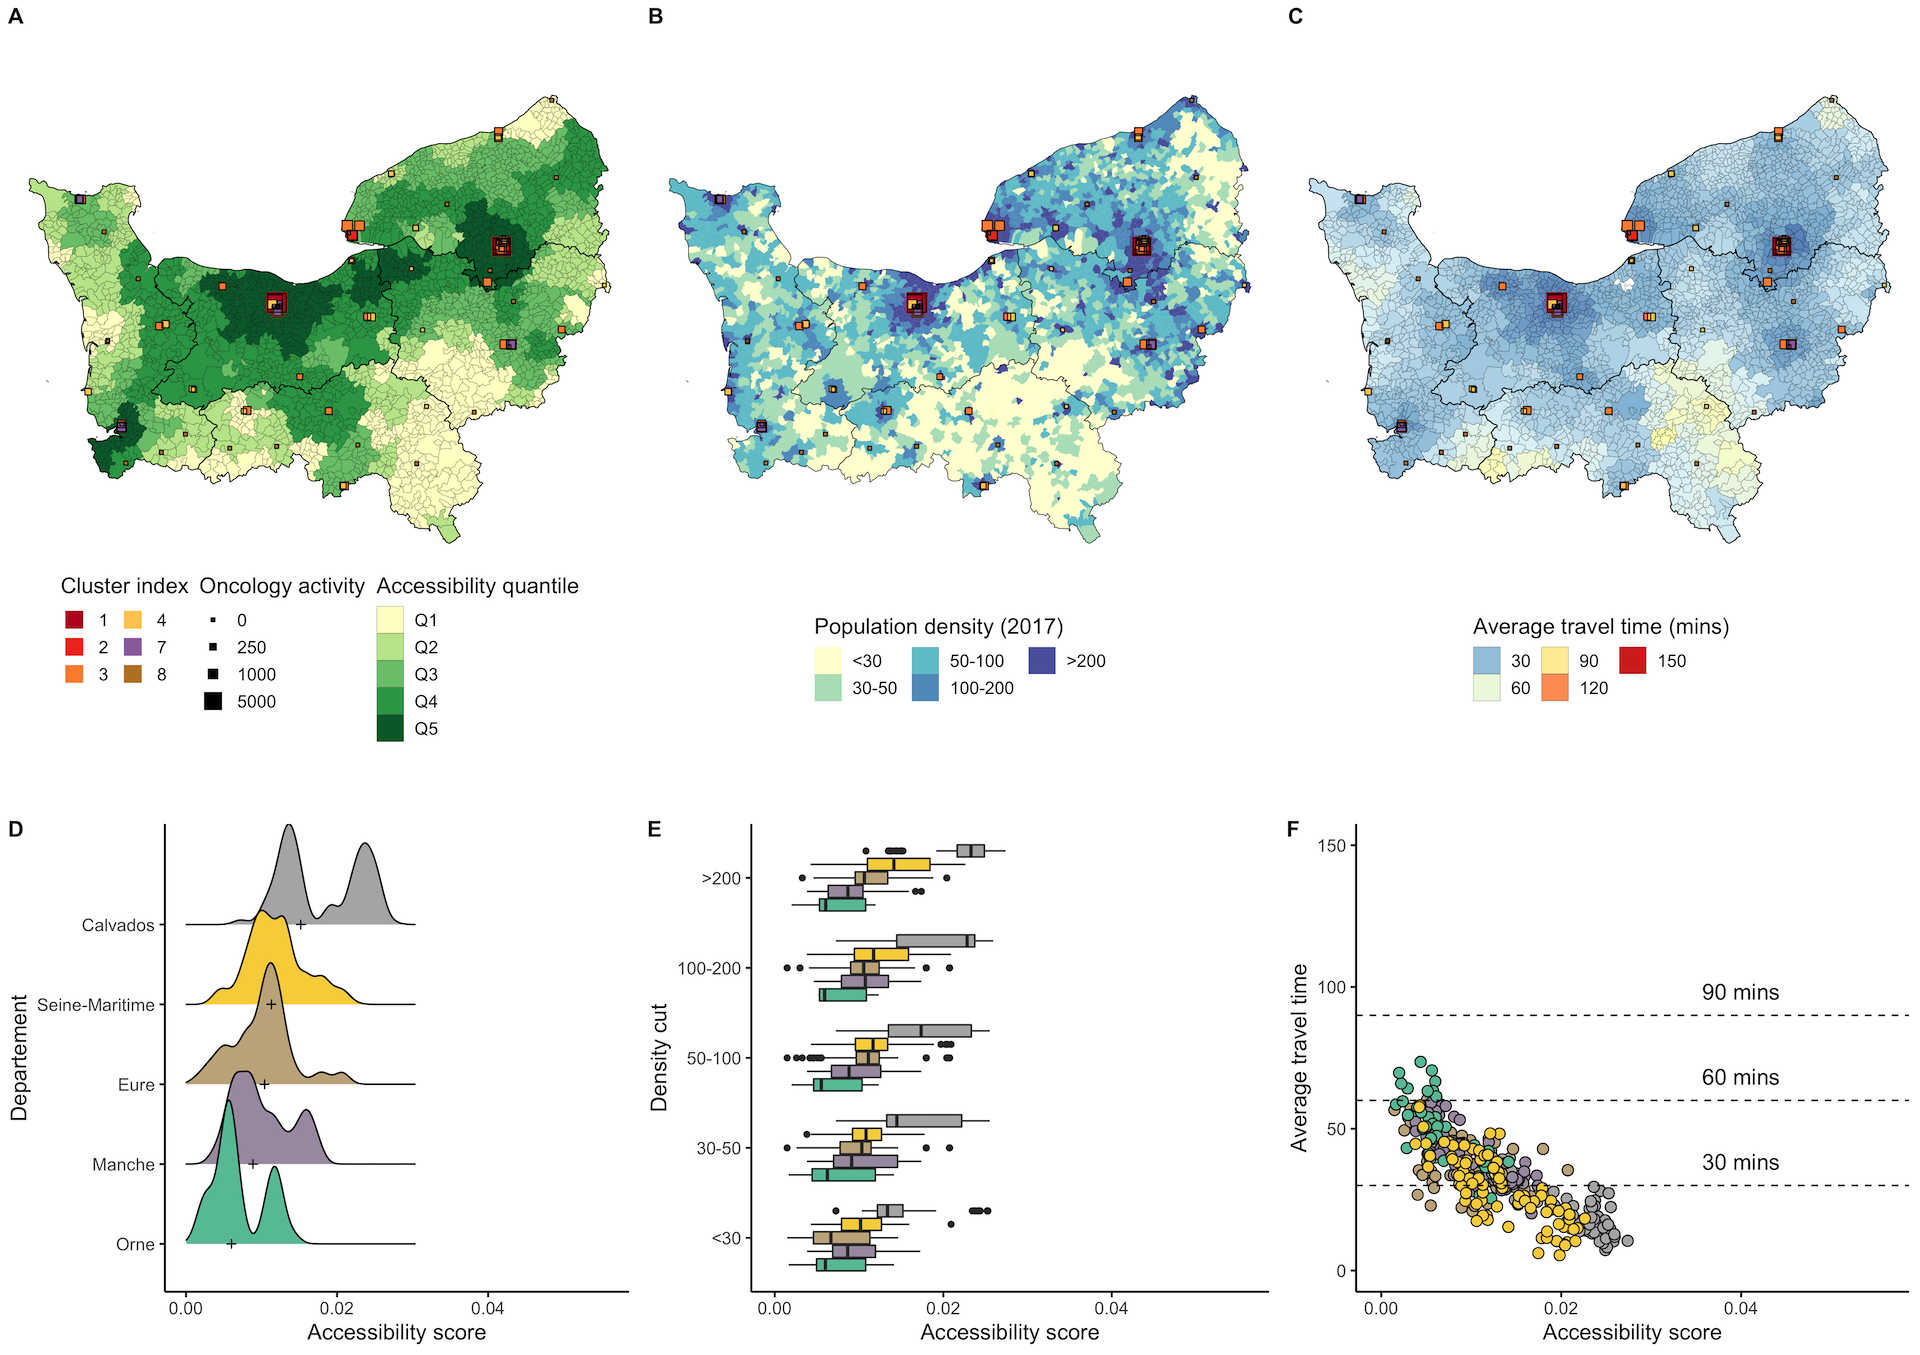
\includegraphics[width=0.9\textwidth]{images/camion/region_accessibility/accessibility_Normandie.png}
    \centering
    \caption{
        \textbf{Accessibility distribution in Normandie.}
    }
\end{figure}

\subsubsection{Accessibility in Île-de-France region}

The Île-de-France (IdF) region is located in the center north of France. This
one covers 12,012 km\textsuperscript{2} for a population of 12,213,447 (Insee)
in 2018. The IdF region is the most populated and dense of metropolitan France.
Only 5\% of the population lives in a rural commune, for the 671 rural communes
cover 59\% of the IdF territory. The majority of rural communes (85\%) are under
the influence of Paris. Île-de-France is composed of 8 departments, 4
departments in the inner suburbs and 4 departments in the outer suburbs. It is a
special region because it includes the French capital, Paris, the leading French
city in terms of demography and population density with 2,175,601 inhabitants in
2021. The city of Paris is also home to many specialized health establishments.
The rural communes are far from the influence of Paris and are mainly located in
the departments of the outer suburbs, three quarters of which are in
Seine-et-Marne. The most rural and least dense areas are therefore mainly
located in the east of the region, particularly along the border to the east of
the Seine-et-Marne department.

Île-de-France has good accessibility over the vast majority of its territory.
Indeed, 63.8\% of the population of IdF is located in an area with a maximum
accessibility score, and almost no population is located in an area with a
minimum accessibility score Q1 or even Q2. Also, although only 9\% of the
territory's surface is identified as having a Q5 score and 15\% as having a Q1
score, the minimum accessibility zones are not very densely populated, which
only affects a very small part of the region's population. Indeed, we observe
that the only areas with a Q1 score are located in the eastern part of the
region in the Seine-et-Marne department where the population density is very
low. Moreover, travel time is uniform throughout the region with a very good
level of travel time limited to an average of 30 minutes. The Ile-de-France
region does not suffer from accessibility difficulties at any level for cancer
treatments, regardless of location in the territory.

\begin{figure}[h!]
    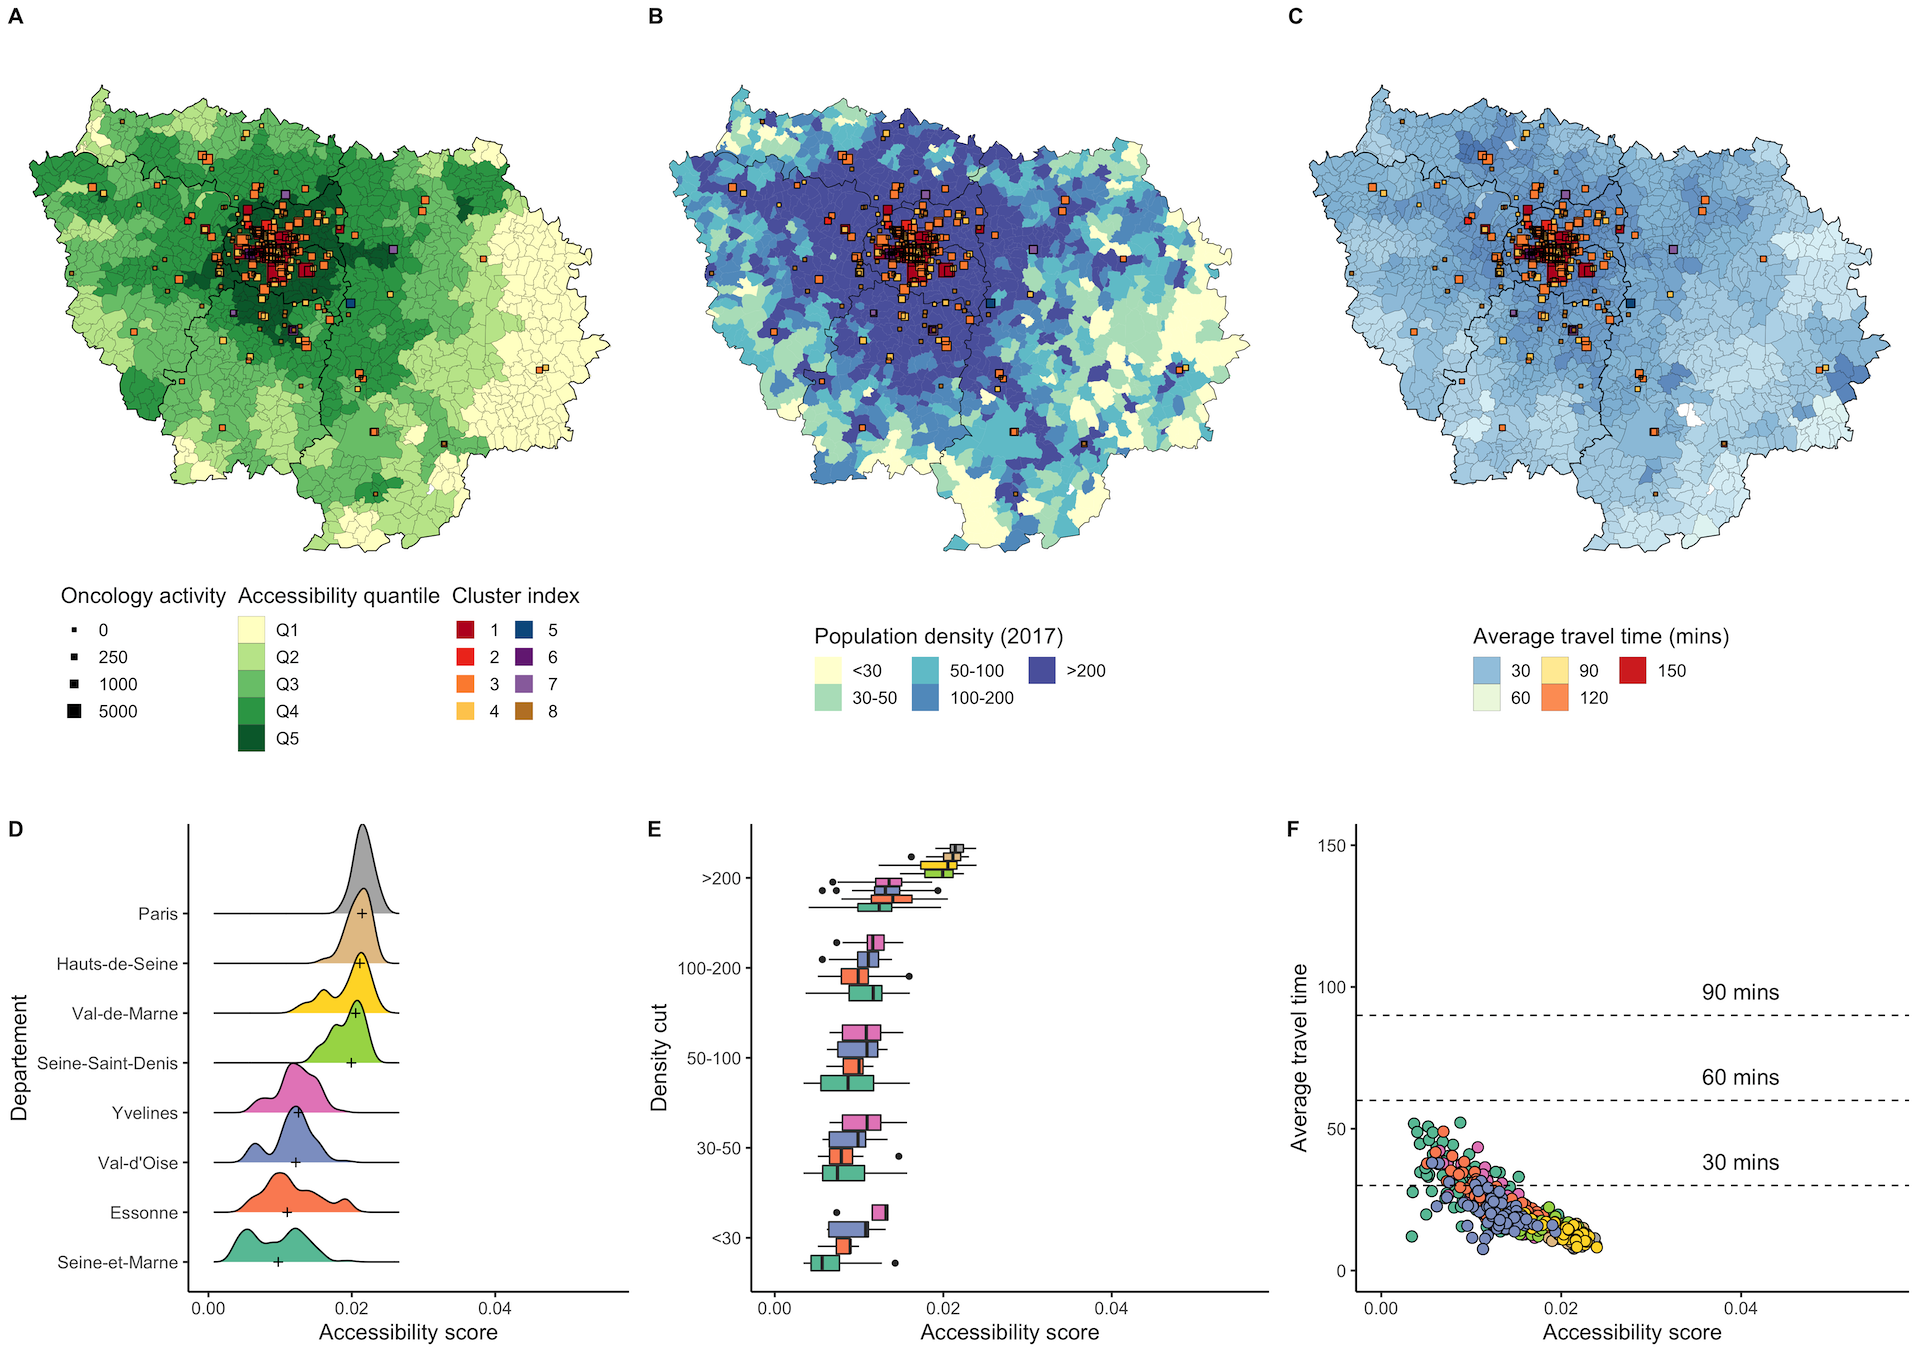
\includegraphics[width=0.9\textwidth]{images/camion/region_accessibility/accessibility_Ile-de-France.png}
    \centering
    \caption{
        \textbf{Accessibility distribution in Ile-de-France.}Île-de-France has good accessibility over the vast majority of its territory.
        Indeed, 63.8\% of the population of IdF is located in an area with a maximum
        accessibility score, and almost no population is located in an area with a
        minimum accessibility score Q1 or even Q2. Also, although only 9\% of the
        territory's surface is identified as having a Q5 score and 15\% as having a Q1
        score, the minimum accessibility zones are not very densely populated, which
        only affects a very small part of the region's population.
    }
\end{figure}

\subsubsection{Accessibility in Hauts-de-France region}

The Hauts-de-France region is located in the north of France. It covers
31,948km² for a population of 6,005,000 (Insee) in 2019, or 9\% of the
metropolitan population. The region has retained a strong industrial footprint.
It is the second most urbanized region after Ile de France with 89\% of its
population living in a large urban area. However, 83\% of the region's
municipalities are considered rural (including autonomous rurality and rurality
under the influence of a pole in a peri-urban area), with 29\% of the region's
population living in a so-called rural municipality. The Hauts-de-France is
composed of 5 departments. In the department of Nord in the north of the region,
particularly urbanized and densified, is the city of Lille which has 1,411,571
inhabitants in its metropolis. Amiens in the department of Somme is the second
most populated urban area in the region.

The accessibility zones are relatively evenly distributed over the territory,
although the best accessibility in this department is mainly in the urban and
peri-urban area of Lille. Travel time averages 30 minutes over most of the
region, with the exception of the northern end of the region in the Aisne
department and the northeastern part of the same department, where travel time
averages 60 to 90 minutes. The population density is also low in these areas,
the Aisne being the least populated department in the Hauts-de-France region.
Only 4.4\% of the population of Hauts-de-France is located in an area with an
accessibility quantile of Q1 and 16.6\% in Q2. It is possible to perceive that
certain parts of the territory with a medium (100-200) to high (>200) population
density have an accessibility qualified at Q2 and Q3, which implies a difficulty
of accessibility of optimal care for certain segments of the population. In
fact, despite a low population rate in Q1, only 32.5\% of the regional
population is located in an area with the highest quantile of accessibility Q5.
These observations allow us to consider that the improvement of accessibility to
optimal care in this territory could be easily optimized because the initial
care offer is already well distributed in the territory with accessibility zones
Q4 and Q3, which together account for 46.4\% of the population.

\begin{figure}[h!]
    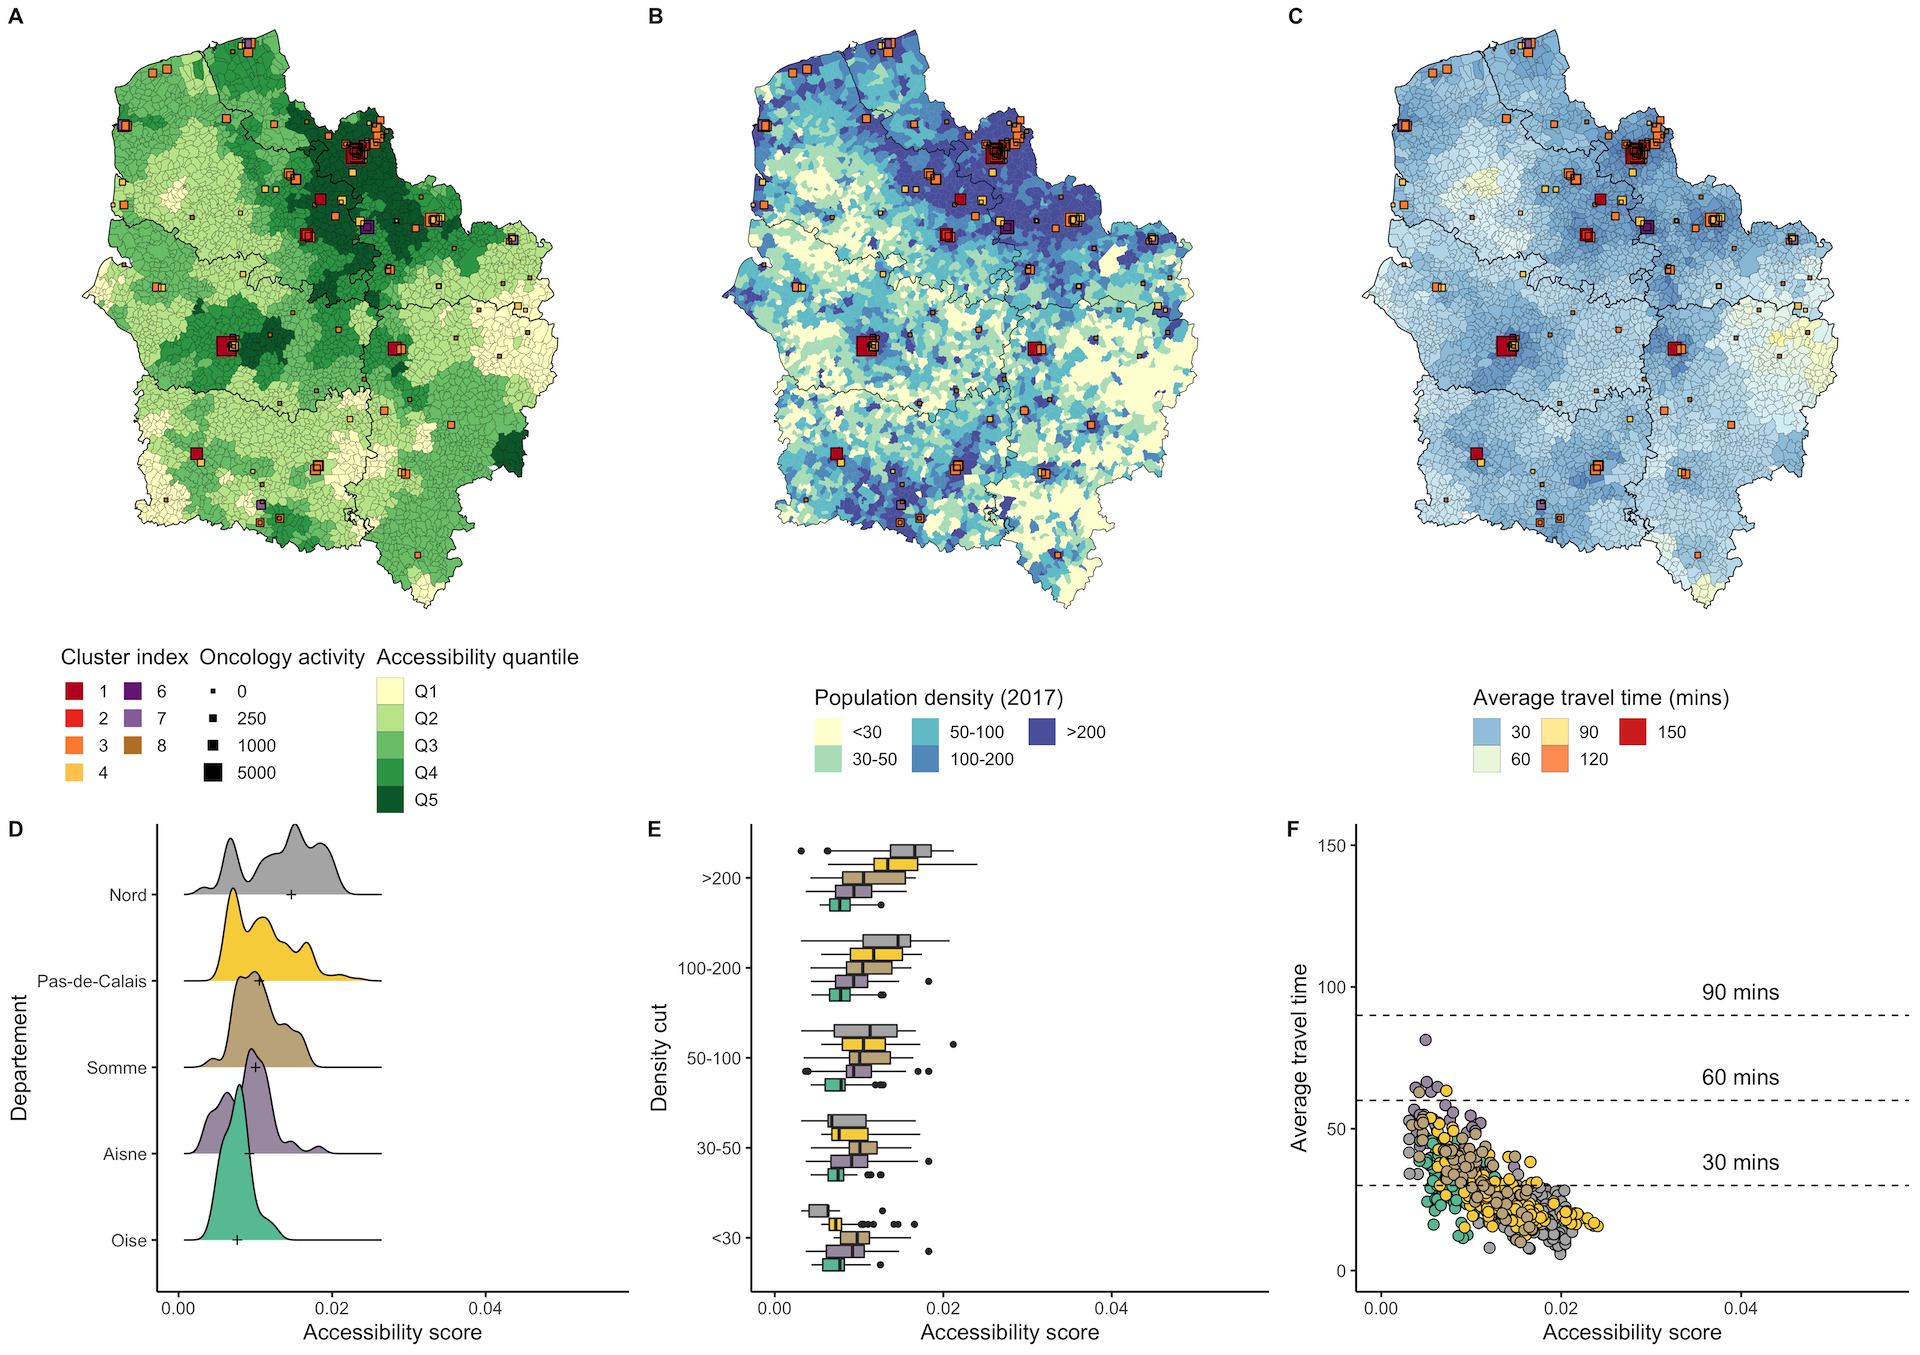
\includegraphics[width=0.9\textwidth]{images/camion/region_accessibility/accessibility_Hauts-de-France.png}
    \centering
    \caption{ \textbf{Accessibility distribution in Hauts-de-France.} The
        accessibility zones are relatively evenly distributed over the
        territory, although the best accessibility in this department is mainly
        in the urban and periurban area of Lille. Travel time averages 30
        minutes over most of the region, with the exception of the northern end
        of the region in the Aisne department and the northeastern part of the
        same department, where travel time averages 60 to 90 minutes }
\end{figure}

\subsubsection{Accessibility in Grand Est region}

The Grand Est region is located in the east of France. It covers 57,433
km\textsuperscript{2} for a population of 5,556,219 (Insee) in 2019. 39\% of the
population resides in a rural commune (i.e., a commune with low or very low
density). 61\% of the population resides in urban areas, 22.8\% in peri-urban
rural areas and 16.2\% in autonomous rural areas, moreover nearly 80\% of the
regional surface is dedicated to agriculture and forestry. The Grand Est is
composed of 8 departments. The departments of Meuse and Haute-Marne central to
the region are among the most rural departments in France with respectively 74\%
and 67\% of their population living in rural areas (peri-urban and autonomous),
while the departments of Haut-Rhin, Bas-Rhin, Meurthe-et-Moselle and Moselle
have more than 60\% of their population living in urban areas (2018, Insee). The
department of Marne in the west of the region is home to Reims, the most densely
populated city in the region after Strasbourg.

The accessibility is high in the eastern half of the region in the departments
of Moselle, Meurthe et Moselle, Bas-Rhin, Haut-Rhin, particularly around the
large agglomerations (Strasbourg, Nancy, Metz, Colmar). Indeed, 41\% of the
population of the Grand Est is in an accessibility zone of Q5 and only 7.5\% in
a Q1 zone. The lack of accessibility in the western part of the region is more
pronounced due to the low or very low density areas that are more common in
these departments. Also, the link between population density and accessibility
is visible and reinforced by the consideration of average travel times. Travel
times are almost uniformly distributed over the entire territory, with little or
no travel time exceeding 30 minutes; travel times of 60 minutes on average are
limited and those of 90 minutes are very limited. These times are most prevalent
in the western half of the region in the very low density areas but mostly in
the less demographically dense areas.  The poor accessibility for the city of
Charles-Ville-Mézière (46,436 inhabitants in 2019) is more worrying in view of
its demographic density. However, it can be observed that the coverage of
maximum accessibility for the majority of the population does not necessarily
require a spatial accessibility spread over the surface of the region, since the
Grand Est has only 13.5\% of the surface of its territory considered as Q5
accessibility, but covers the needs of maximum accessibility for 41\ of its
population. Thus, the urban nature of the population of the Grand Est seems to
be a determining factor in maximizing accessibility to care.

\begin{figure}[h!]
    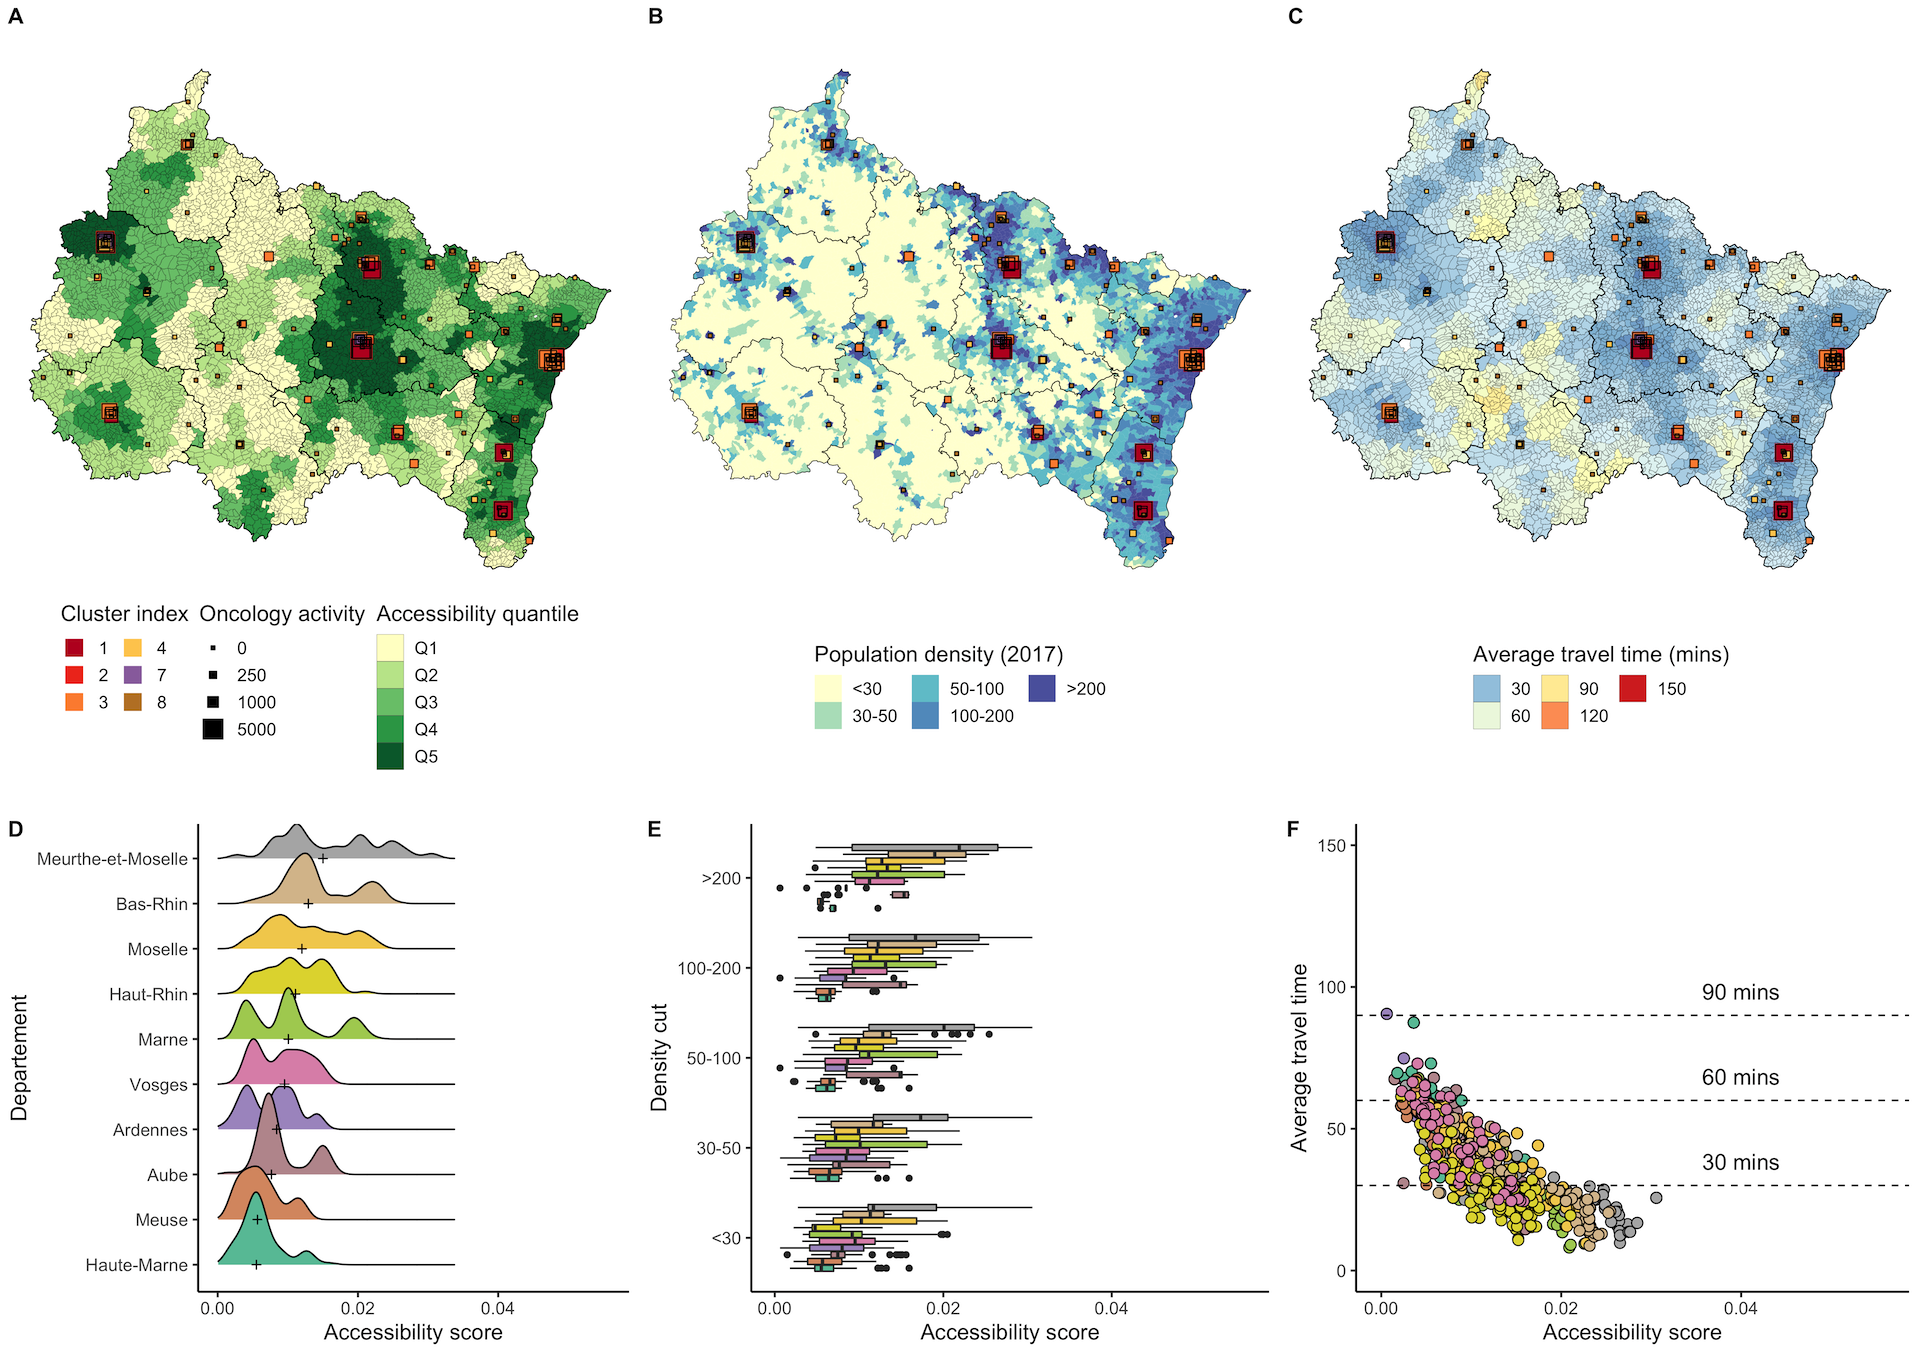
\includegraphics[width=0.9\textwidth]{images/camion/region_accessibility/accessibility_Grand-Est.png}
    \centering
    \caption{ \textbf{Accessibility distribution in Grand-Est.} We notice good
        accessibility scores in the eastern half of the region in the
        departments of Moselle, Meurthe et Moselle, Bas-Rhin, Haut-Rhin,
        particularly around the large agglomerations (Strasbourg, Nancy, Metz,
        Colmar). Indeed, 41\% of the population of the Grand Est is in an
        accessibility zone of Q5 and only 7.5\% in a Q1 zone. The lack of
        accessibility in the western part of the region is more pronounced due
        to the low or very low density areas that are more common in these
        departments. }
\end{figure}

\subsubsection{Accessibility in Centre-Val de Loire region}

The Centre-Val-de-Loire region is located in the center west of France. It
covers an area of 39 151 km\textsuperscript{2} with a population of 2 573 180
(Insee) in 2019. The region is one of the most rural regions of France, with
90\% of its territory occupied by rural municipalities and 1 in 2 inhabitants
living in a rural municipality (49\%). 27\% of the population (700,000
inhabitants) live in a rural commune under the influence of a major pole and
nearly 22\% (of 570,000) outside the area of attraction of such a pole. However,
the CVdL includes two metropolitan areas, Orléans in the department of Loiret
and Tour in Indre-et-Loire, which together account for one-third of the regional
population. Paris also has an influence on the region, affecting 184,000
inhabitants under its influence, i.e., 7\% of the CVdL population. Thus, the
majority of the population (90\%) lives in an attractive urban area. The
Hauts-de-France is made up of 6 departments. The department of Indre-et-Loire
includes and Loiret includes the two metropolitan areas of the region Tour with
137,665 inhabitants and Orleans with 288,229 inhabitants in 2019.

The accessibility of the whole region is relatively lower than in other regions
observed so far. Many areas have a low or very low accessibility score despite a
medium population density. Areas with low or very low population density can
have a very low accessibility score, although low-density areas of the Cher have
a score around the Q3 quantile. Only the city of Tour and its vicinity shows a
maximum level of accessibility, as well as some surrounding parcel areas in the
department of Loir-et-Cher around the city of Blois and in the department of
Cher around Bourges. Even the city of Orleans has an accessibility score of Q4
despite the presence of level 1 clusters. The CVdL has the particularity of
being the only French region without a \ac{clcc} on its territory. The closest
\ac{clcc} are those in adjacent regions, in Paris in the Île-de-France and Anger
in Normandy. We can deduce that in order to access a specialized center, the
inhabitants of this region have to leave the region.  We can see that the level
1 clusters in the region are located in Tour, Orléans and Chartes. The
departments in the south of the region have lower level clusters, with the Cher
having only a level 3 and a level 7 cluster. This is reflected in the travel
times which are rather homogeneous and low in the northern and central
departments with average travel times of 30 minutes, while the southern
departments, Indre and Cher have much higher travel times throughout their
territory, around 60 minutes and 90 minutes.

\begin{figure}[h!]
    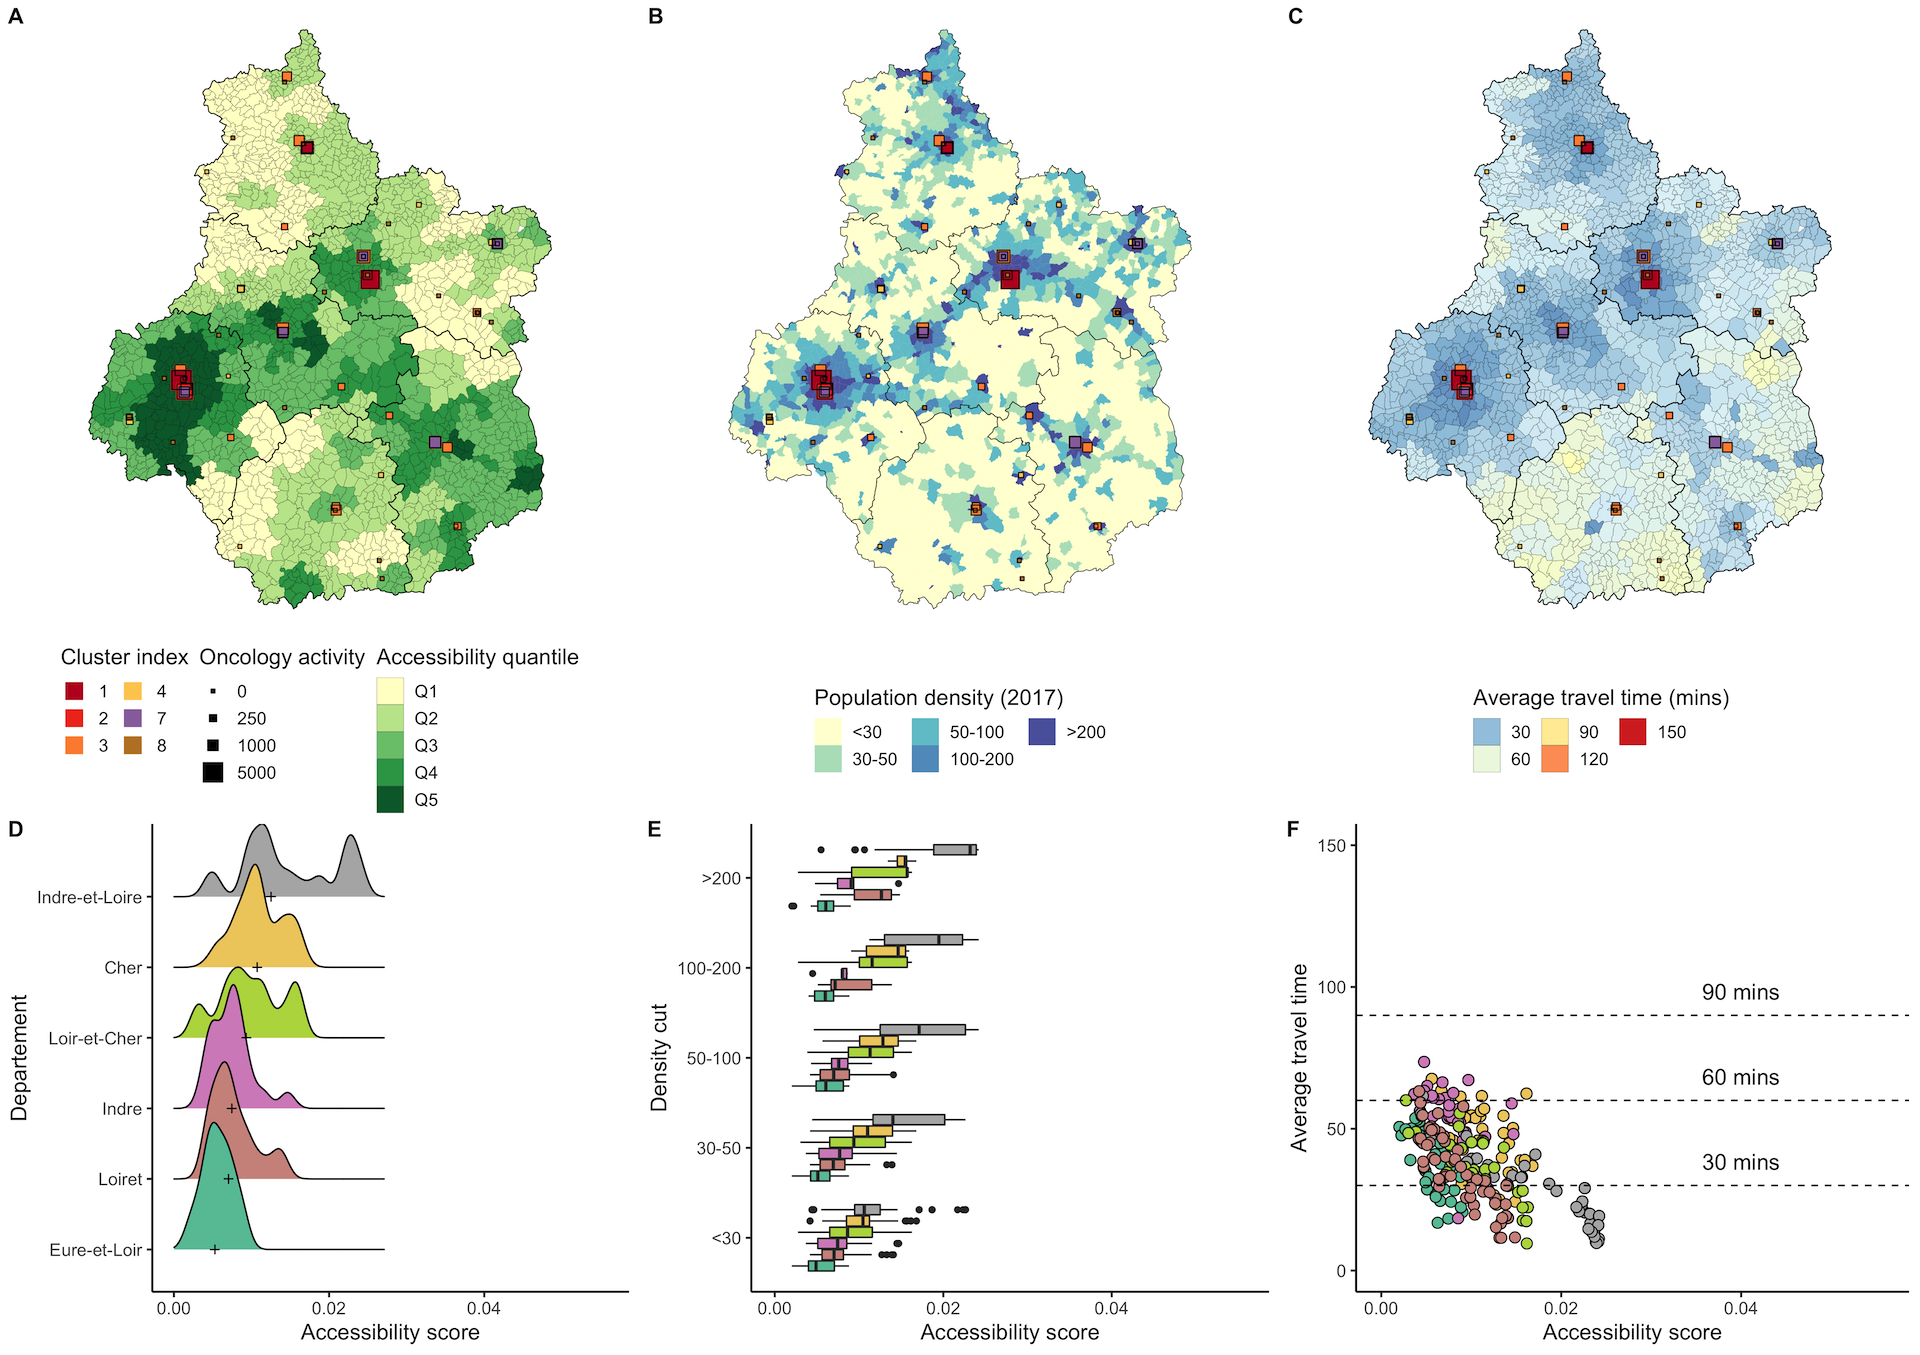
\includegraphics[width=0.9\textwidth]{images/camion/region_accessibility/accessibility_Centre-Val-de-Loire.png}
    \centering
    \caption{ \textbf{Accessibility distribution in Centre Val de Loire.} The
        accessibility of the whole region is relatively lower than in other
        regions observed so far. Many areas have a low or very low accessibility
        score despite a medium population density. Areas with low or very low
        population density can have a very low accessibility score, although
        low-density areas of the Cher have a score around the Q3 quantile. Only
        the city of Tour and its vicinity shows a maximum level of
        accessibility, as well as some surrounding parcel areas in the
        department of Loir-et-Cher around the city of Blois and in the
        department of Cher around Bourges. }
\end{figure}

\subsubsection{Accessibility in Bretagne region}

The region of Bretagne is located in the west of France, on the Atlantic coast.
It covers 27,208 km², making it the largest region in France, with a population
of 3,354,854 (Insee) in 2019. More than half of the Breton population (53.7\%)
resides in a rural commune, so Bretagne is the second most rural region of
metropolitan France after Burgundy-Franche-Comté. The Breton rural area is
characterized by longer travel times to everyday services. 25.7\% of the
inhabitants of very sparsely populated autonomous areas have to travel more than
10 minutes on average to access them, and for 68.6\% of them, the average
journey takes between 7 and 10 minutes. However, a major part of the population
lives in an attractive urban area, i.e. 87\% of the region's population.
Bretagne is composed of 5 departments. The main metropolis of the region is
Rennes with 215,366 inhabitants and 364,133 inhabitants in its urban unit, the
first agglomeration of the department of Ille-et-Vilaine, followed by Brest
which is located in the department of Finistère with 139,926 inhabitants.

Bretagne has very good accessibility with 57.7\% of its population living in a
territory with maximum accessibility and above all a very low rate of its
population in territories with low or very low accessibility with 5.1\% of its
population in Q2 and only 1.5\% of its population in Q1. Also, the maps show a
good distribution of accessibility throughout the territory, with variations
often related to the territory's population density ratio. Travel times reflect
the level of accessibility, with many travel times less than 30 minutes and some
travel times between 30 and 60 minutes but very rarely more. However, Morbihan
has a relatively high proportion of trips between 30 and 60 minutes, including
rare areas where travel times exceed 90 minutes, particularly due to the
department's profile, which includes certain islands such as Belle-Île, which
have travel times of over 120 minutes.


\begin{figure}[h!]
    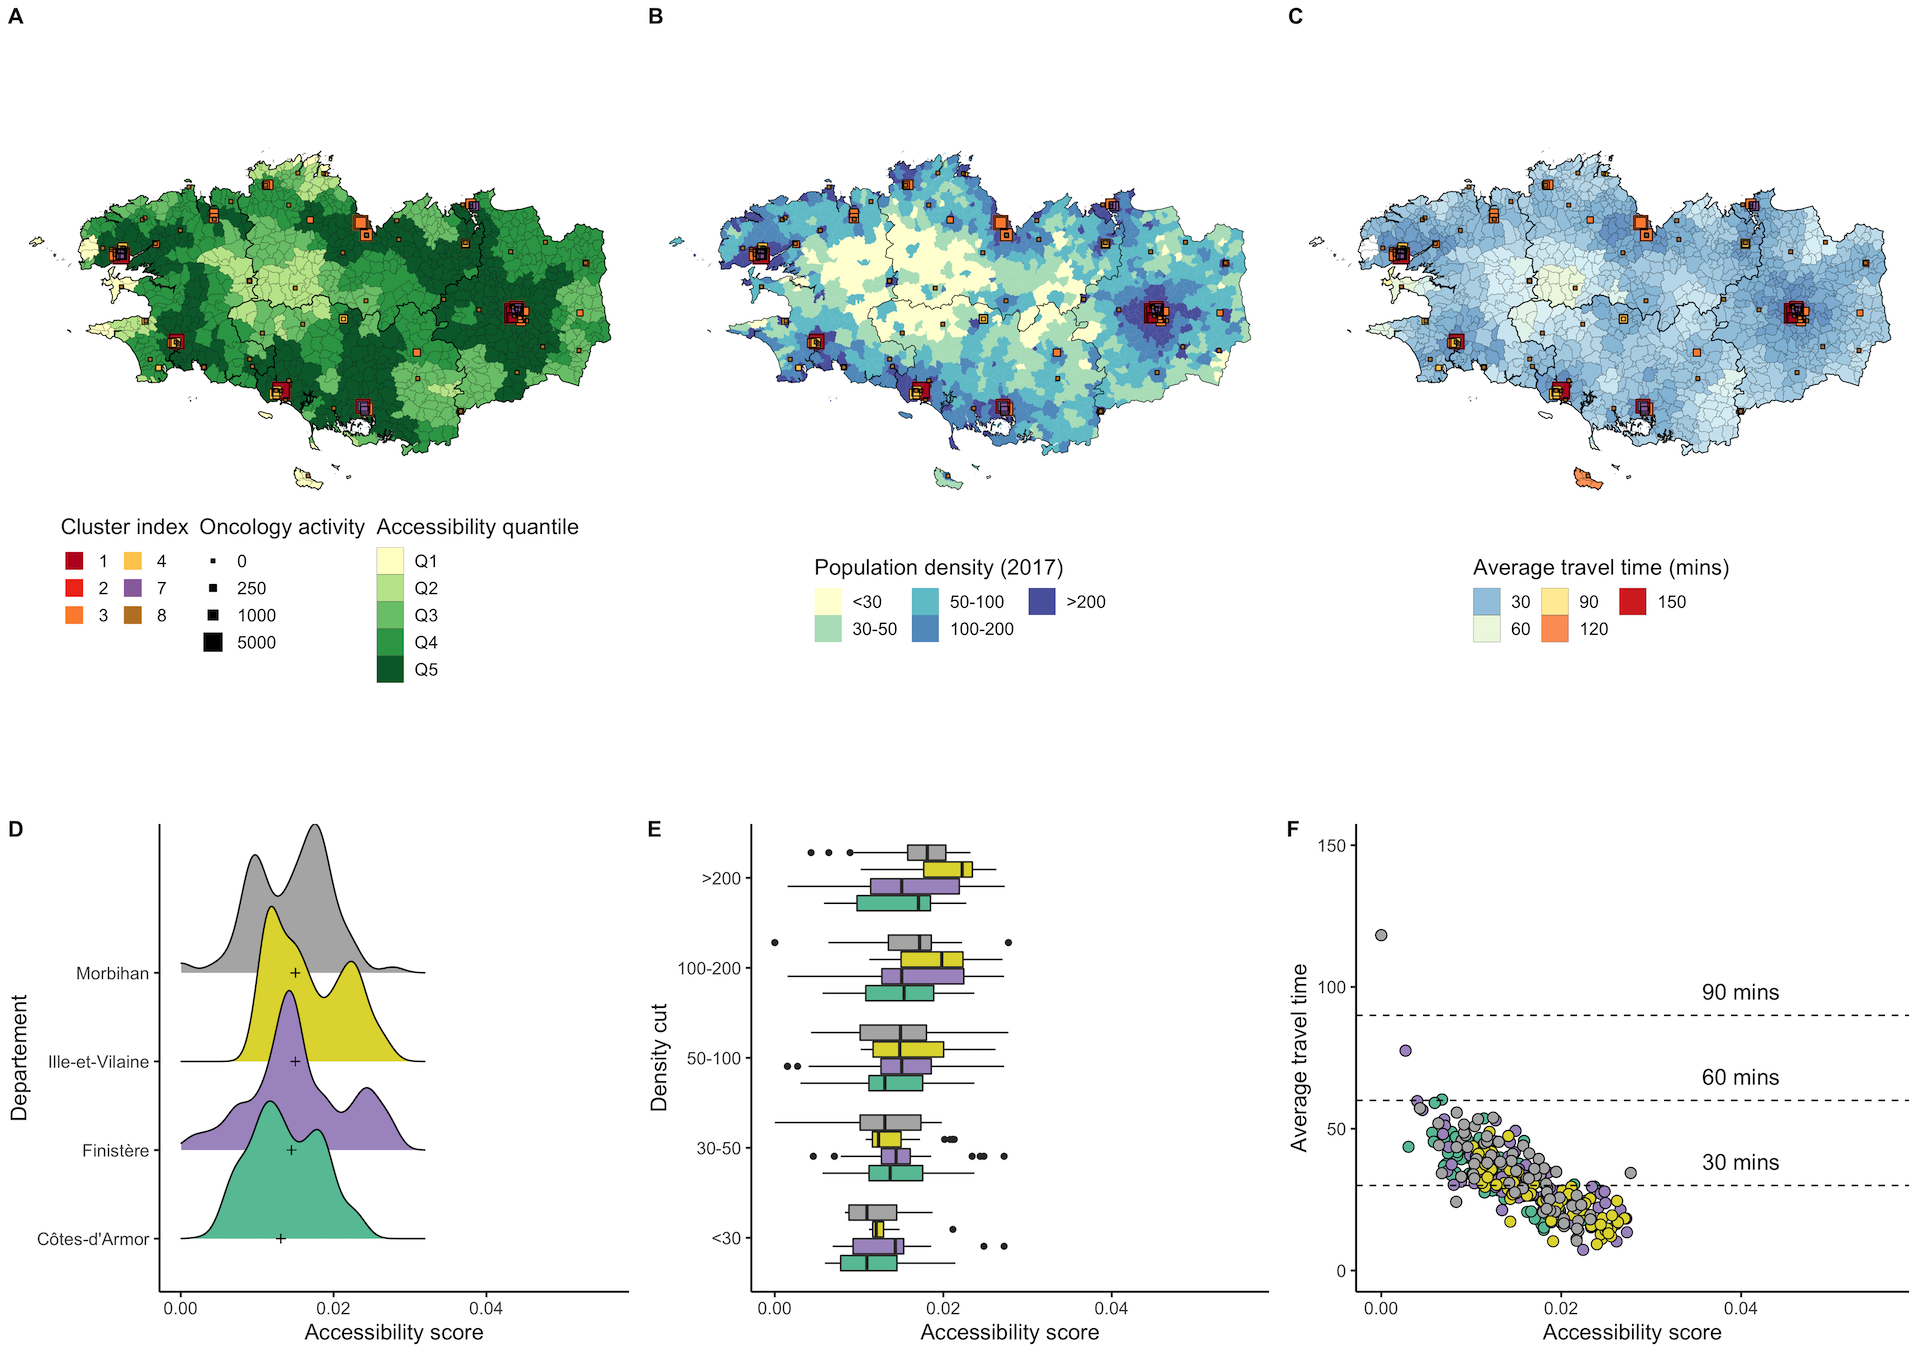
\includegraphics[width=0.9\textwidth]{images/camion/region_accessibility/accessibility_Bretagne.png}
    \centering
    \caption{
        \textbf{Accessibility distribution in Bretagne.}
    }
\end{figure}

\subsubsection{Accessibility in Bourgogne-Franche-Comté region}

The Bourgogne-Franche-Comté (BFC) region is located in the center-east of
France. It covers 47,784 km\textsuperscript{2} for a population of 2,805,580
(Insee) in 2019 with 1,242,882 active people. In 2018 the BFC is considered the
first rural region of France with more than half of its population (1.5 million
people) residing in rural areas. The BFC is composed of 8 departments. The
departments of Yvonne, Nièvre to the west, Saône-et-Loire and Jura to the south,
have a particularly rural and agricultural landscape without dense urban areas,
especially for Saône-et-Loire.  In the department of Côte-d'Or is located Dijon,
the largest and most densely populated city in the region with 158,002
inhabitants, ahead of the city of Besançon with its 117,912 inhabitants, which
is located to the east in the department of Doub. In total, the BFC region has
3,704 municipalities, 26 of which have more than 10,000 inhabitants.

The departments of Côte-d'Or and Doubs have the best accessibility, especially
around densely populated urban areas such as Dijon or Besançon. Some areas of
the region have a low accessibility quantile Q1 and Q2 which cover 37.3\% and
16.4\% respectively of the regional territory, i.e. more than half (53.7\%) of
the area is recognized with a level of accessibility to cancer care. The areas
with low or very low accessibility are located mainly in rural areas and with
low or very low population density, except for the eastern border of the Doubs,
which has more densely populated areas, but with more mountainous terrain, with
a quantile 1 accessibility. In each department, accessibility is best in the
urban areas and their surroundings. The travel time shows an unequal
distribution of access to health care in the territory, since the majority of
municipalities have an average travel time of 30 minutes, but large areas of the
region show average travel times of 60 or 90 minutes, particularly in the
departments of Nièvre and Yvonne, although in the less densely populated areas
of these departments, or travel times exceeding 120 minutes in the east of the
Jura at the Swiss border, which is, however, likely to be a more mountainous
terrain

\begin{figure}[h!]
    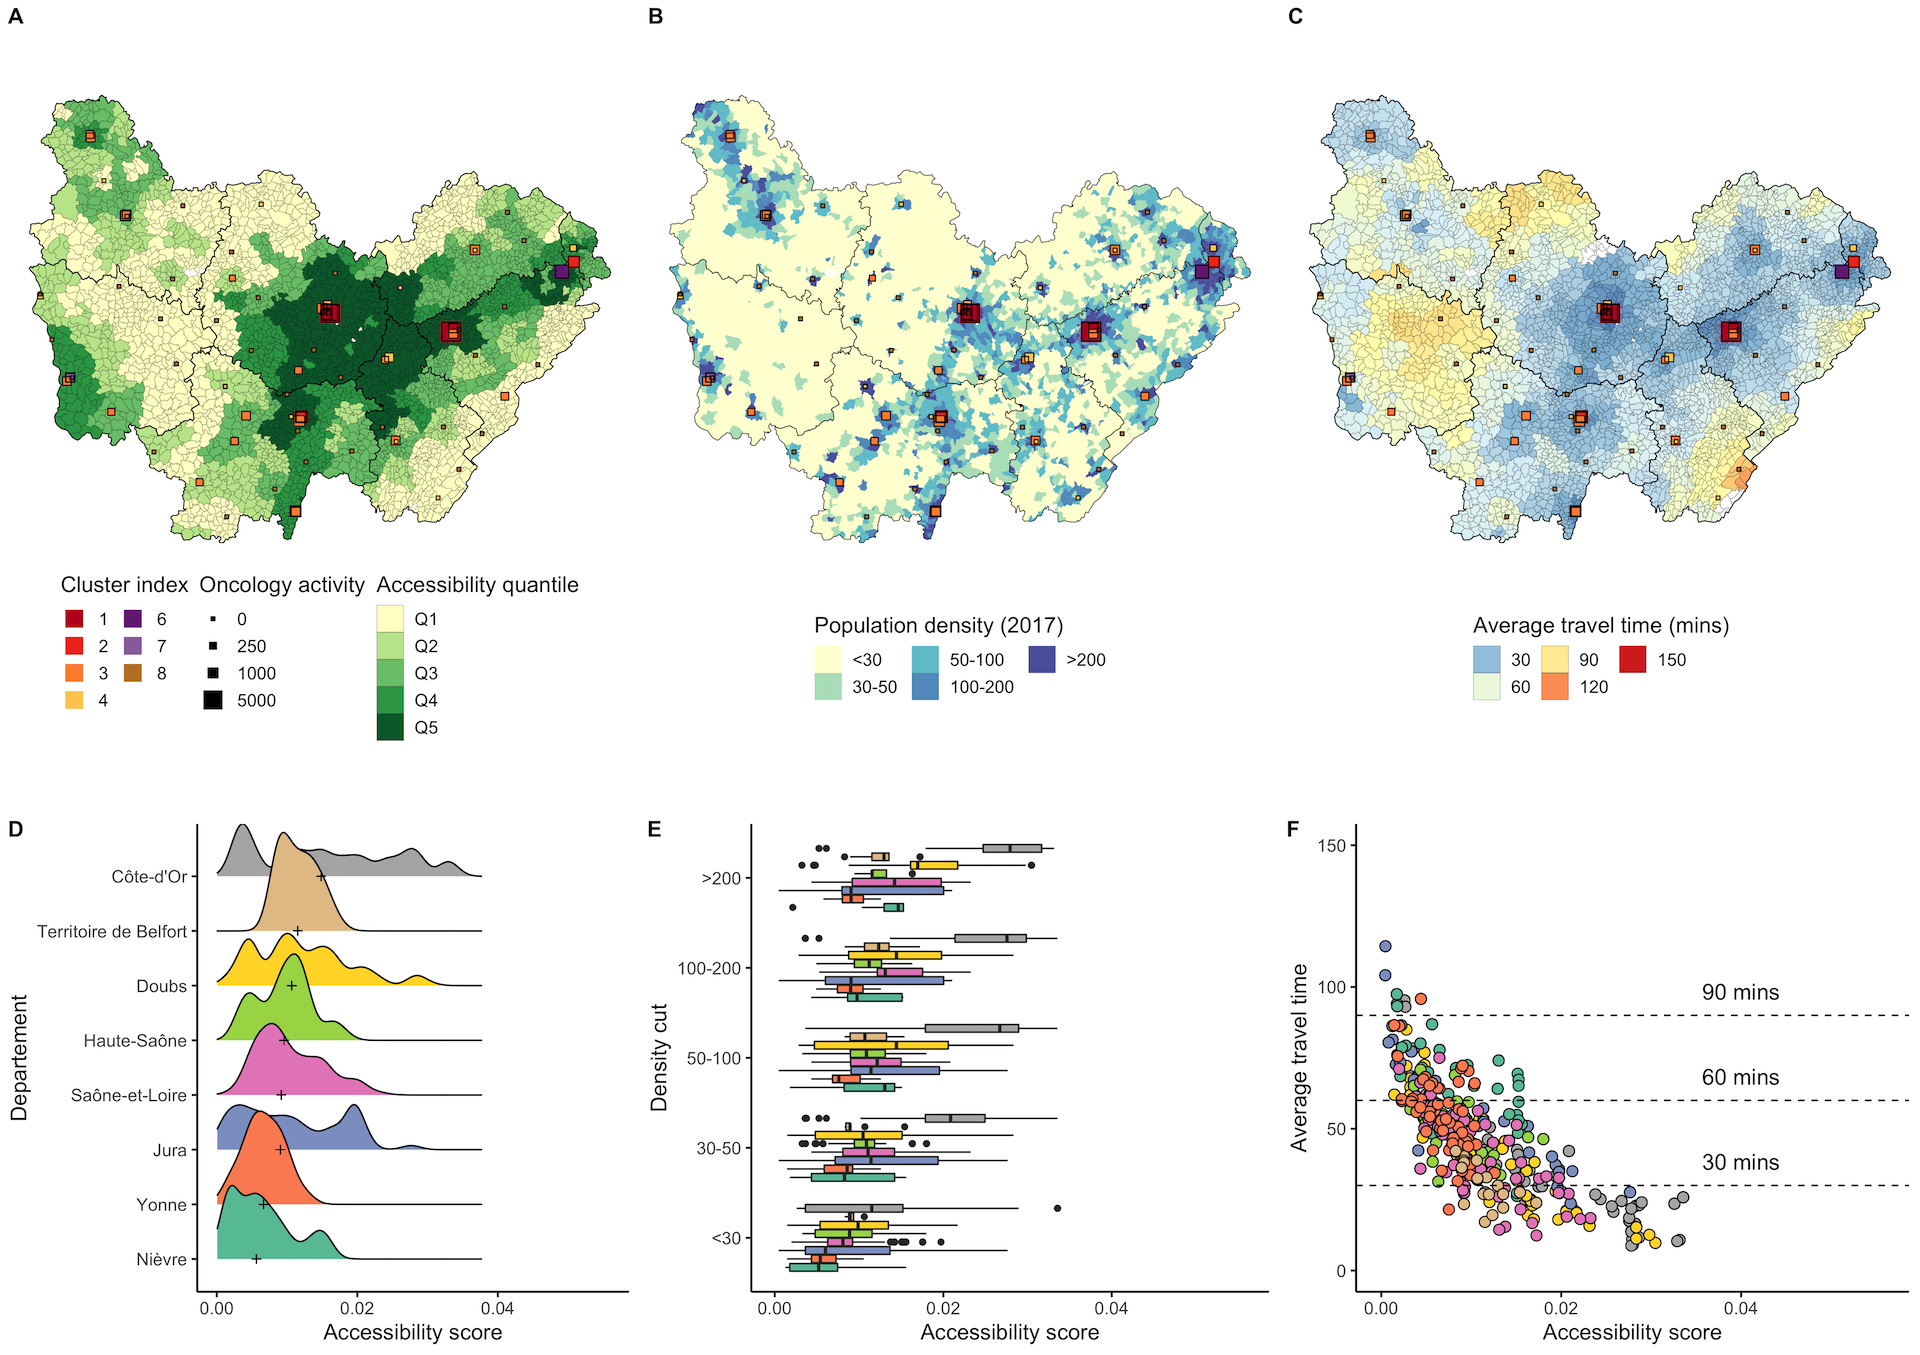
\includegraphics[width=0.9\textwidth]{images/camion/region_accessibility/accessibility_Bourgogne-Franche-Comte.png}
    \centering
    \caption{ \textbf{Accessibility distribution in Bourgogne-Franche-Comté.}
        The departments of Côte-d'Or and Doubs have the best accessibility,
        especially around densely populated urban areas such as Dijon or
        Besançon. Some areas of the region have a low accessibility quantile Q1
        and Q2 which cover 37.3\% and 16.4\% respectively of the regional
        territory, i.e. more than half (53.7\%) of the area is recognized with a
        level of accessibility to cancer care. The areas with low or very low
        accessibility are located mainly in rural areas and with low or very low
        population density, except for the eastern border of the Doubs, which
        has more densely populated areas, but with more mountainous terrain,
        with a quantile 1 accessibility. }
\end{figure}

\subsubsection{Accessibility in Auvergne-Rhône-Alpes region}

The Auvergne-Rhône-Alpes (ARA) region is located in eastern France. It covers
69,711 km\textsuperscript{2} for a population of 7,994,459 (Insee) in 2018,
representing 12.3\% of the metropolitan population, i.e. the most populated
region in France. The ARA is the main mountain region of France with 2.2 million
people residing in a municipality classified as a mountain area, with more than
half in the regional part of the Massif Central which is distributed in a
diagonal of low population density, while the population of the Alpine massif is
concentrated in the urbanized and more densely populated parts at the bottom of
valleys. In the ARA, 35\% of the population lives in a rural commune, the
provincial metropolitan average being 33\%, and these communes cover 89\% of the
region's surface area. The ARA is composed of 12 departments. The Rhône
department in the northern center of the region includes the city of Lyon, the
second largest city in France, which has 1,411,571 inhabitants in its
metropolis. The eastern departments, Savoie, Haute-Savoie, Isère, Drôme,
constitute the mountainous areas of the region. Of the twelve departments, five
are considered 'essentially rural': Cantal (74\% of the inhabitants live in
rural communes), Haute-Loire (70\%), Ardèche (60\%), Allier (58\%) and Ain
(50\%).

If we look at the maps, we can see that the areas with the lowest accessibility
are mainly located in areas with low or very low density, particularly along the
mountainous border in the east of the region in the departments of Haute-Savoie,
Savoie, Isère and Drôme. It is possible to observe a good distribution of
accessibility in the central, northern and north-western part of the region,
particularly around the large agglomerations such as the city of Lyon,
Clermont-Ferrand, Moulins, Grenoble and Aurillac. The three southern
departments, Haute-Loire, Ardèche and Drôme, are less accessible than the other
departments in the region. Above all, it can be observed that the mountainous
terrain tends to have a strong impact on accessibility to care, since travel
times in these areas, particularly for the departments of Drôme and Savoie,
reach an average of 120 minutes if not 150 minutes. In the mountainous
departments of the east, the valleys that contain the urban centers with the
highest population density, such as Chambéry, Grenoble and Annecy, are the most
favorable accessibility centers in these departments. Despite its mountainous
nature, 51.1\% of the Auvergne-Rhône-Alpes region is located in an accessibility
zone Q5 compared to 8\% in an accessibility zone Q1.

\begin{figure}[h!]
    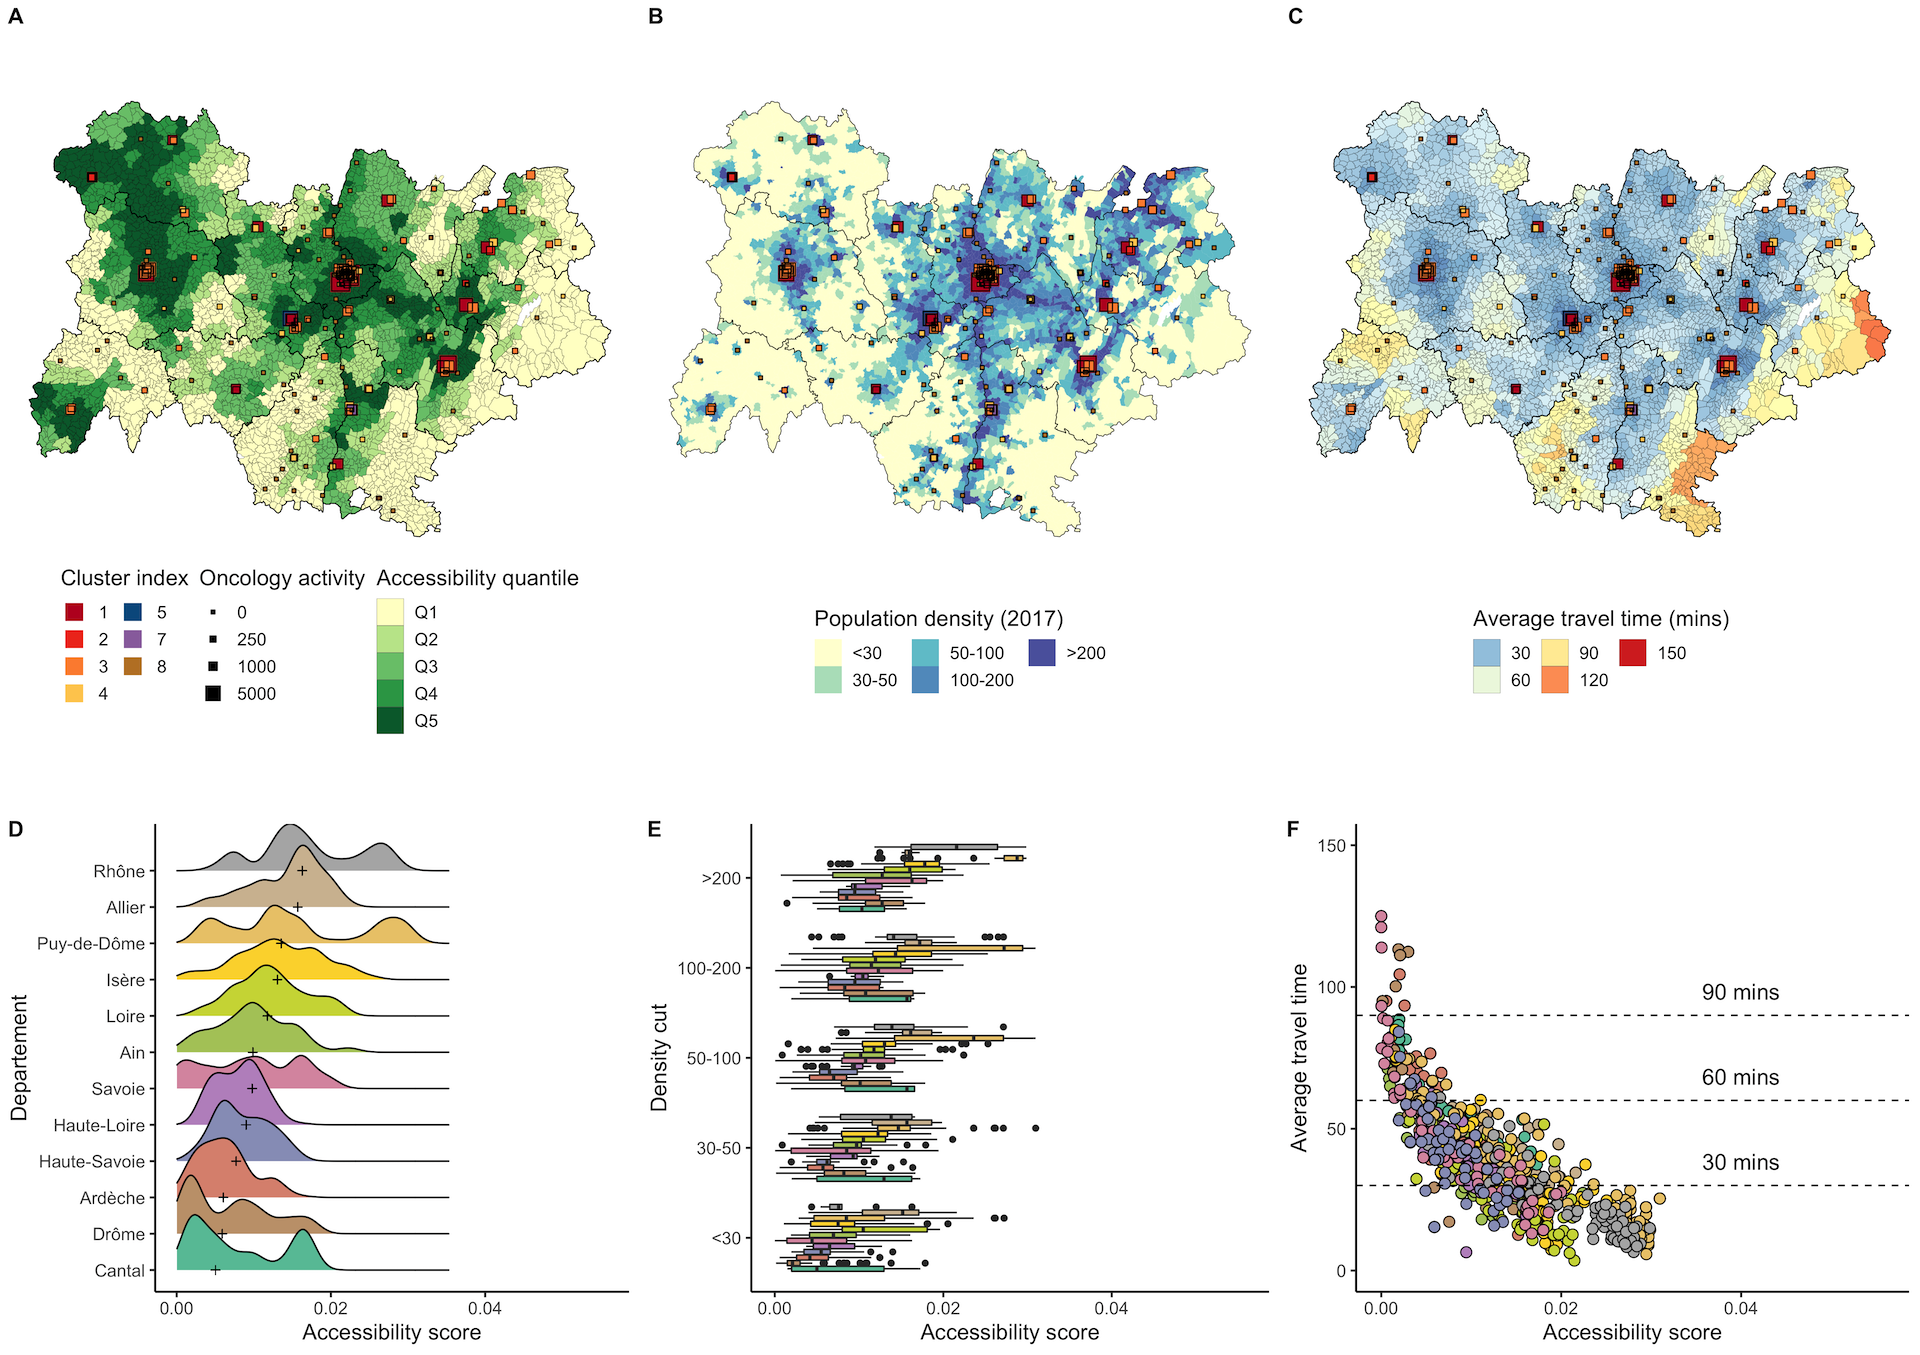
\includegraphics[width=0.9\textwidth]{images/camion/region_accessibility/accessibility_Auvergne-Rhone-Alpes.png}
    \centering
    \caption{ \textbf{Accessibility distribution in Auvergne-Rhone-Alpes.} The
        areas with the lowest accessibility are mainly located in areas with low
        or very low density, particularly along the mountainous border in the
        east of the region in the departments of Haute-Savoie, Savoie, Isère and
        Drôme. It is possible to observe a good distribution of accessibility in
        the central, northern and north-western part of the region, particularly
        around the large agglomerations such as the city of Lyon,
        Clermont-Ferrand, Moulins, Grenoble and Aurillac. The three southern
        departments, Haute-Loire, Ardèche and Drôme, are less accessible than
        the other departments in the region. Above all, it can be observed that
        the mountainous terrain tends to have a strong impact on accessibility
        to care, since travel times in these areas, particularly for the
        departments of Drôme and Savoie, reach an average of 120 minutes if not
        150 minutes. }
\end{figure}

\section{Conclusion}

In this section, we described our method to compute the oncology accessibility
score given to every municipality in metropolitan France. This score was
obtained by using the \acf{e2sfca} algorithm, with oncology activity as supply,
municipality population as demand, and driving car duration as impedance metric.
Specific attention should be given to municipalities with very poor access to
oncology care centers. While we saw that most of the population lives in high
accessibility areas, around 6\% of the population lives in the bottom 20\%
accessibility quantile. Among these municipalities, some are very rural and
mountainous like those in the Alpes-de-Haute-Provence in
Provence-Alpes-Cote-d'Azur region. Such areas cannot be expected to have a very
good healthcare coverage. By contrast, the case of suburban areas with
relatively dense population and poor accessibility should be addressed more
easily. Our optimization algorithm can help driving public health policies, as
it effectively identifies areas where accessibility could grow, by allocating
additional oncology activity to a restricted number of care centers. The
proposed growth factors are indicative and do not have to be effective within a
year, as it represents a considerable effort for care centers to increase their
activity. Our oncology accessibility score is deliberately non-specific to
cancer type. This score is meant to outline how easy it would be for a
population location to reach a first entry point for oncology care. Here, we are
only focusing on surgery, chemotherapy, and radiotherapy treatments. The same
technique could be used on a specific cancer type, the method will remain the
same, only the supply variable used in the accessibility score will change. We
should mention that \ac{sa} is better suited for pathologies that are relatively
well handled across the whole country. Accessibility for rare diseases like
pediatric cancer or complex cancers that re-quire a specific expertise is less
informative because only a handful of care centers are indicated. Similarly, we
could compute an accessibility score that is focused on specific kinds of stays:
our web application lets the user pick between surgery, chemotherapy, or
radiotherapy as supply variable.

  \chapter{CAMION: Catchment Area MaximizatION algorithm}

\section{Context}

\subsection{Motivation}

Uneven distributions of population and health-care providers lead to geographic disparity in accessibility for patients \cite{wang_why_2020}. For instance, Weiss et al. \cite{weiss_global_2020} showed that 8.9\% of the global population could not reach healthcare within one hour if they have access to motorized transport. In Germany, Bauer et al. \cite{bauer_spatial_2020} shown that 10\% of the population lived in areas with low accessibility for internal medicine and surgery. Location-allocation algorithms \cite{church_location_1999} can optimize the distribution and supply of health providers to reduce accessibility disparities. These algorithms seek the optimal placement of facilities for a desirable objective under certain constraints \cite{wang_measurement_2012}. For instance, Luo et al. developed an optimization algorithm to improve the healthcare planning in rural China by finding the best place and capacity for new health facilities \cite{luo_integrating_2014}. Tao et al. worked on a spatial optimization model to maximize equity in accessibility to residential care facility in Beijing, China \cite{tao_spatial_2014}. When optimizing health accessibility, there are two competing goals: equity and efficiency \cite{krugman_opinion_2013,meyer_equity_2008}. Equity may be defined as equal access to healthcare for everyone \cite{culyer_equity_1993}. An efficient situation is when everything has been done to help any person without harming anyone else \cite{hemenway_optimal_1982}. While some argue that efficiency should be ad-dressed in priority \cite{hemenway_optimal_1982}, others agree that equity is a matter of ethical obligation, especially in public health \cite{fried_rights_1975, oliver_equity_2004}.

\subsection{Location-allocation algorithms}

Regarding efficiency optimization, the most popular algorithms are p-median, \ac{lscp} and \ac{mclp}. The p-median algorithm minimizes the weighted sum of distances between users and facilities \cite{murad_using_2021}. \ac{lscp} minimizes the number of facilities needed to cover all demand \cite{shavandi_fuzzy_2006}. \ac{lscp} maximizes the demand covered within a desired distance or time threshold by locating a given number of facilities \cite{casado_heuristical_2005}.
To reach equal access to healthcare, quadratic programming has been used to  minimize the variance of accessibility scores defined by the \ac{2sfca} \cite{wang_planning_2013}. Similarly, a \ac{pso} algorithm was developed to minimize the total square difference between the accessibility score of each demand location and the weighted average accessibility score \cite{tao_spatial_2014}. Finally, a two-step optimization algorithm has been developed to address the dual objectives of efficiency and equality, by first choosing where to site new hospitals and then deciding which capacity they should have \cite{luo_two-step_2017,li_two-step_2017}.

\section{Methods}

However, most of the previous algorithms seek locations to open new health facilities. In this work, we are interested in the case where the health facilities are fixed, and the only lever to improve accessibility is to increase their capacities. Given a capacity budget, we want to know which facilities to grow and by how much. We introduce \ac{camion}, an accessibility optimization algorithm based on \ac{fca} and \ac{lp}. The initial accessibility score was computed with the \ac{e2sfca} algorithm \cite{luo_enhanced_2009} but our algorithm can generalize to more \ac{fca} derivatives.
We model the problem as an optimization task. In our case, we want our optimization algorithm to find new care centers capacities given some constraints, so that the total accessibility is maximum. We apply optimization on a given region only, rather than on the whole metropolitan France. We chose this approach because healthcare planning is handled regionally rather than nationally. We show below that our optimization problem is a \ac{lp} problem.
In its standard form, \ac{lp} finds a vector $x$ that maximizes $c^T x$ under constraints $Ax \leq b$, where $A$ is a matrix and $b$ a vector. Boundaries can be set to $x$ such as $x \geq 0$. Consider $x_u$ the new capacity of a care center $u$, to be computed by the algorithm. Let $Q_u$ and $W_u$ be two vectors of size $m$, defined as follows:

\begin{align}
    Q_u &=  \sum_{s=1}^{r} W_s \sum_{i, d_{iu} \in I_s} P_i \\[10pt]
    W_u &=  \sum_{s=1}^{r} \sum_{i, d_{iu} \in I_s} W_s
\end{align}

We can compute the total accessibility as a sum on the m care centers:

\begin{align*}
    \sum_{i} A_i &= \sum_{i} \sum_{s=1}^{r} W_s \sum_{u, d_{iu} \in I_s} \frac{S_u}{Q_u} \\[10pt]
    \sum_{i} A_i &= \sum_{i} \sum_{i, d_{iu} \in I_s} W_s \frac{S_u}{Q_u} \\[10pt]
    \sum_{i} A_i &= \sum_{u} \frac{S_u}{Q_u} \sum_{s} \sum_{i, d_{iu}} W_s \\[10pt]
    \sum_{i} A_i &= \sum_{u} \frac{S_u}{Q_u} W_u \numberthis \label{eq:A_i_sum_u}
\end{align*}

\cref{eq:A_i_sum_u} can be rewritten in the \ac{lp} standard form with:

\begin{align*}
c &= \frac{W_u}{Q_u} \\
x_u &= S_u  \\
b &\geq \sum_{u} x_u  \\
x_{u_\text{min}} &\leq x_u \leq x_{u_\text{max}}
\end{align*}

The user-defined parameters are $b$, $x_{u_\text{min}}$ and $x_{u_\text{max}}$. $b$ is the total capacity to be shared across all the care centers. $x_{u_\text{min}}$ and $x_{u_\text{max}}$ are the capacity boundaries for care center $u$. If $b$ is set to the current total capacity, a care center can’t be grown unless another one is decreased. If $b > \sum_{u} x_u$, the capacity of care centers can be increased without decreasing other centers. We know how to solve \ac{lp} and we used the SciPy \cite{virtanen_scipy_2020} implementation of the revised simplex method as explained in \cite{bertsimas_introduction_1998}.
We now detail how we set the user-defined parameters to apply the \ac{lp} algorithm to our specific case. The additional capacity was set as +3\% of the overall activity of the region's care centers: $b = 1.03 \times \sum_{u} x_u$. The choice of the boundaries $x_{u_\text{min}}$  and $x_{u_\text{max}}$ is crucial and must be realistic. We studied the hospitals activity on the past four years (2016 to 2019) to retrieve the average growth percentage of a care center. The growth percentage is computed as follows: $(S_\text{2019} - S_\text{2016}) / S_\text{2016}$ . Among the care centers that grew and who had an existing oncology activity, the mean growth percentage was 23\%. Hence, we set $x_{u_\text{max}}$ as +20\% of the care center capacity. Regarding $x_{u_\text{min}}$, we set the boundary based on the cluster of the care center. For the three most specialized clusters, we set their $x_{u_\text{min}}$ equal to their current activity. We did this to prevent the algorithm from decreasing the most specialized and well-equipped care centers. Regarding the care centers from the other clusters, $x_{u_\text{min}}$, so that they could be emptied if need be. Finally, we set $x_{u_\text{max}}$ if the care center belongs to the least specialized cluster. The new capacities are indicative and should be further investigated to make sure they are relevant. Especially when setting an existing oncology activity to 0.

\section{Results}

Since we focused on describing the accessibility situation in Provence-Alpes-Cote-d'Azur, we now present the outcomes of our optimization algorithm in this same region. The algorithm was run with the user-specified parameters stated in the Methods Section: we chose to increase the overall oncology activity in the region by 3\% (+3,221 activity) and capped care centers to a 20\% maximum growth. The median accessibility in the region went from 0.0093 to 0.0103, a 11.1\% increase. The results are shown on \cref{fig:optim-paca}. Map (A) displays the accessibility delta ($A_{i_\text{after}} - A_{i_\text{before}}$) as well as the care centers eligible to grow. Centers from cluster 8 were hidden since we considered that they couldn't provide any oncology activity. The algorithm identified a list of 26 care centers where the oncology activity could grow to maximize the total accessibility in the region. These centers are either public or private hospitals, primarily located in the Avignon and Gap areas. The care centers located in high accessibility areas near Marseille and Nice were ignored by the algorithm because improving these zones is not a priority. The care center that grew the most is Clinique Sainte Catherine, in Avignon. Interestingly, this care center was recently bought by the Unicancer group, which coordinates all the cancer centers in France. This hospital's type will change to become a new \ac{clcc}. Thus, it is expected to grow in the next years and to be equipped with more oncology services and staff.

\begin{figure}[h]
    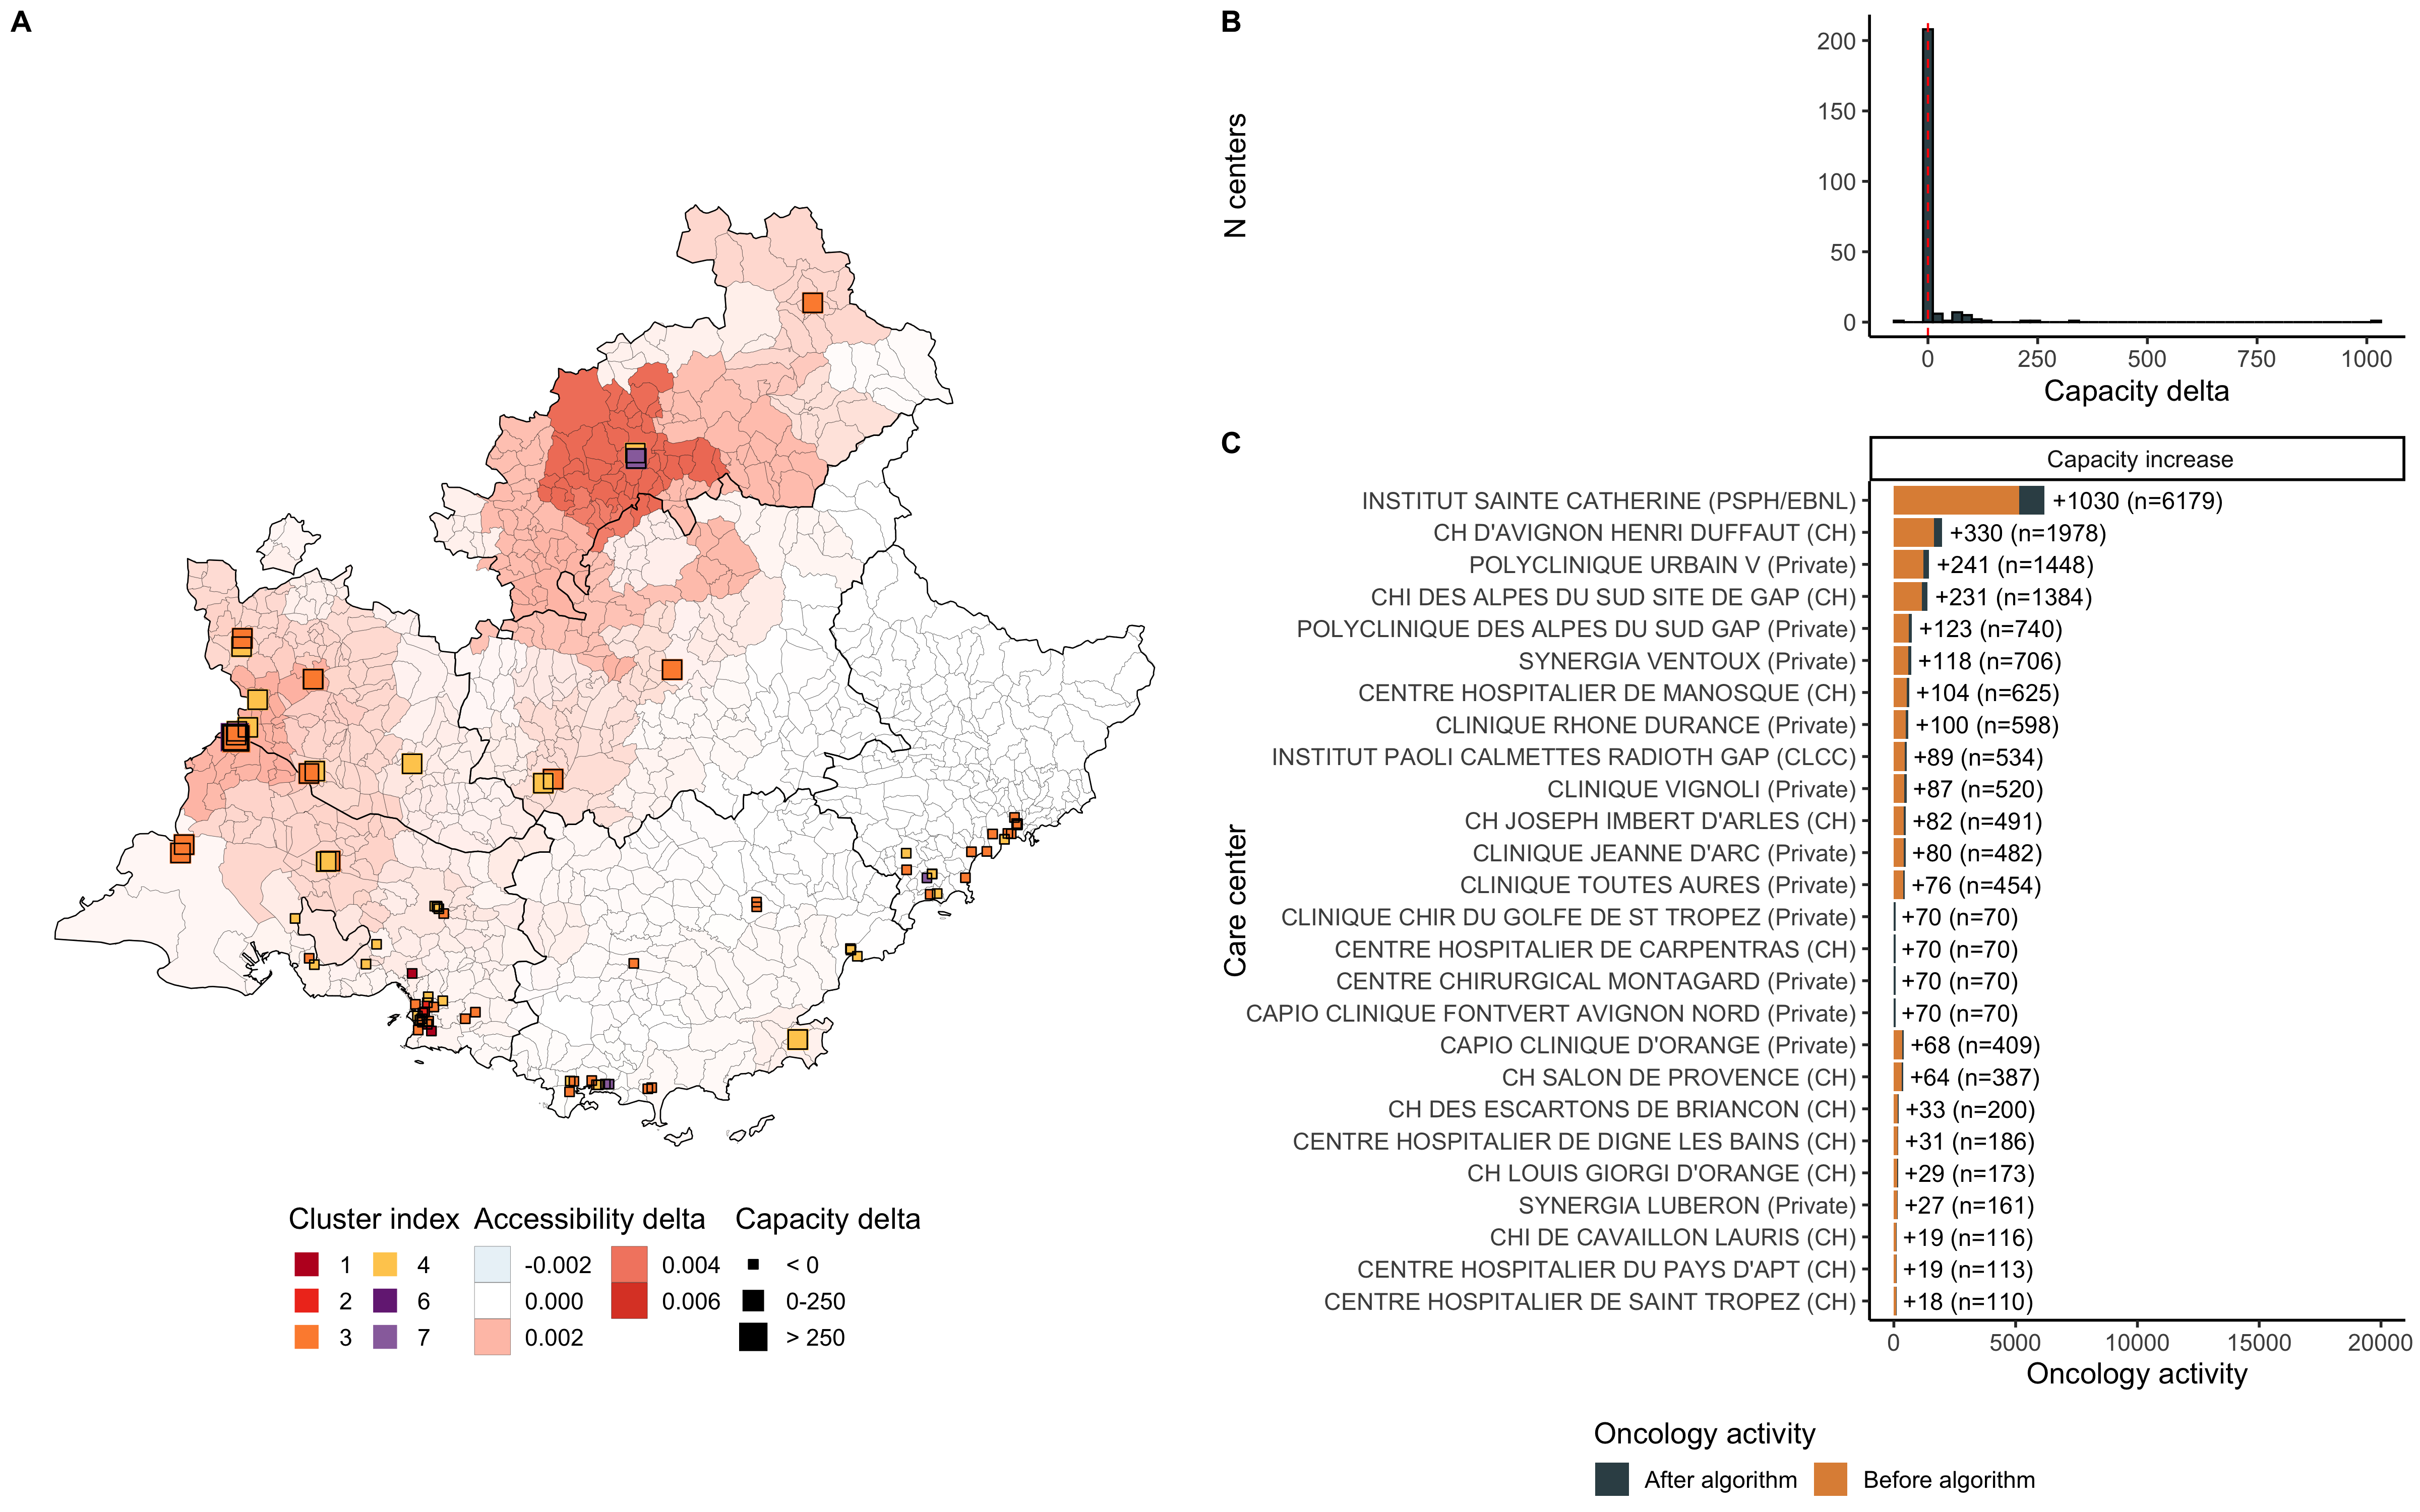
\includegraphics[width=\textwidth]{images/camion/fig5_Provence-Alpes-Cote-d'Azur.png}
    \centering
    \caption{
        Accessibility delta in Provence-Alpes-Cote-d'Azur region after running the optimization algorithm. Map (A) displays the accessibility delta ($A_{i_\text{after}} - A_{i_\text{before}}$) by municipality. Plot (B) shows the capacity delta ($S_{u_\text{after}}-S_{u_\text{before}}$) distribution. Capacity was defined as the oncology activity: the number of patients with chemotherapy or radiotherapy and the number of medical or surgery stays related to oncology. We show the list of the care centers that grew the most (C)  and by how much. For instance, the hospital Institut Sainte Catherine in Avignon, was assigned a +1,030 capacity, for a total of n=6,179. Additional activity was 3,221. 26 centers grew and 1 decreased. Median accessibility before optimization was 0.0093 and 0.0103 after, corresponding to a 11.1\% increase.  Accessibility increased around cities like Avignon and Gap. Care centers near Nice were left unchanged by the algorithm.
    }
    \label{fig:optim-paca}
\end{figure}

While we described the results in Provence-Alpes-Cote-d'Azur region, we ran the algorithm with similar parameters on every region in metropolitan France. We observe two types of optimization strategies. For most regions, the algorithm manages to find a couple of areas where the accessibility can be locally improved, like it did in Provence-Alpes-Cote-d'Azur near Gap and Avi-gnon. However, for regions like Ile-de-France and Haut-de-France, the hospital capacity increase is more uniformly distributed across the region. Most of the time, the algorithm left un-touched the large care centers located in dense cities with good accessibilities. This can be explained by the relatively low value of the additional activity parameter: with a very large value of additional activity, every care center will grow. If we keep it low, the algorithm identifies in which areas hospital capacity should be increased in priority.

\subsection*{Pays de la Loire}

\begin{figure}[h]
    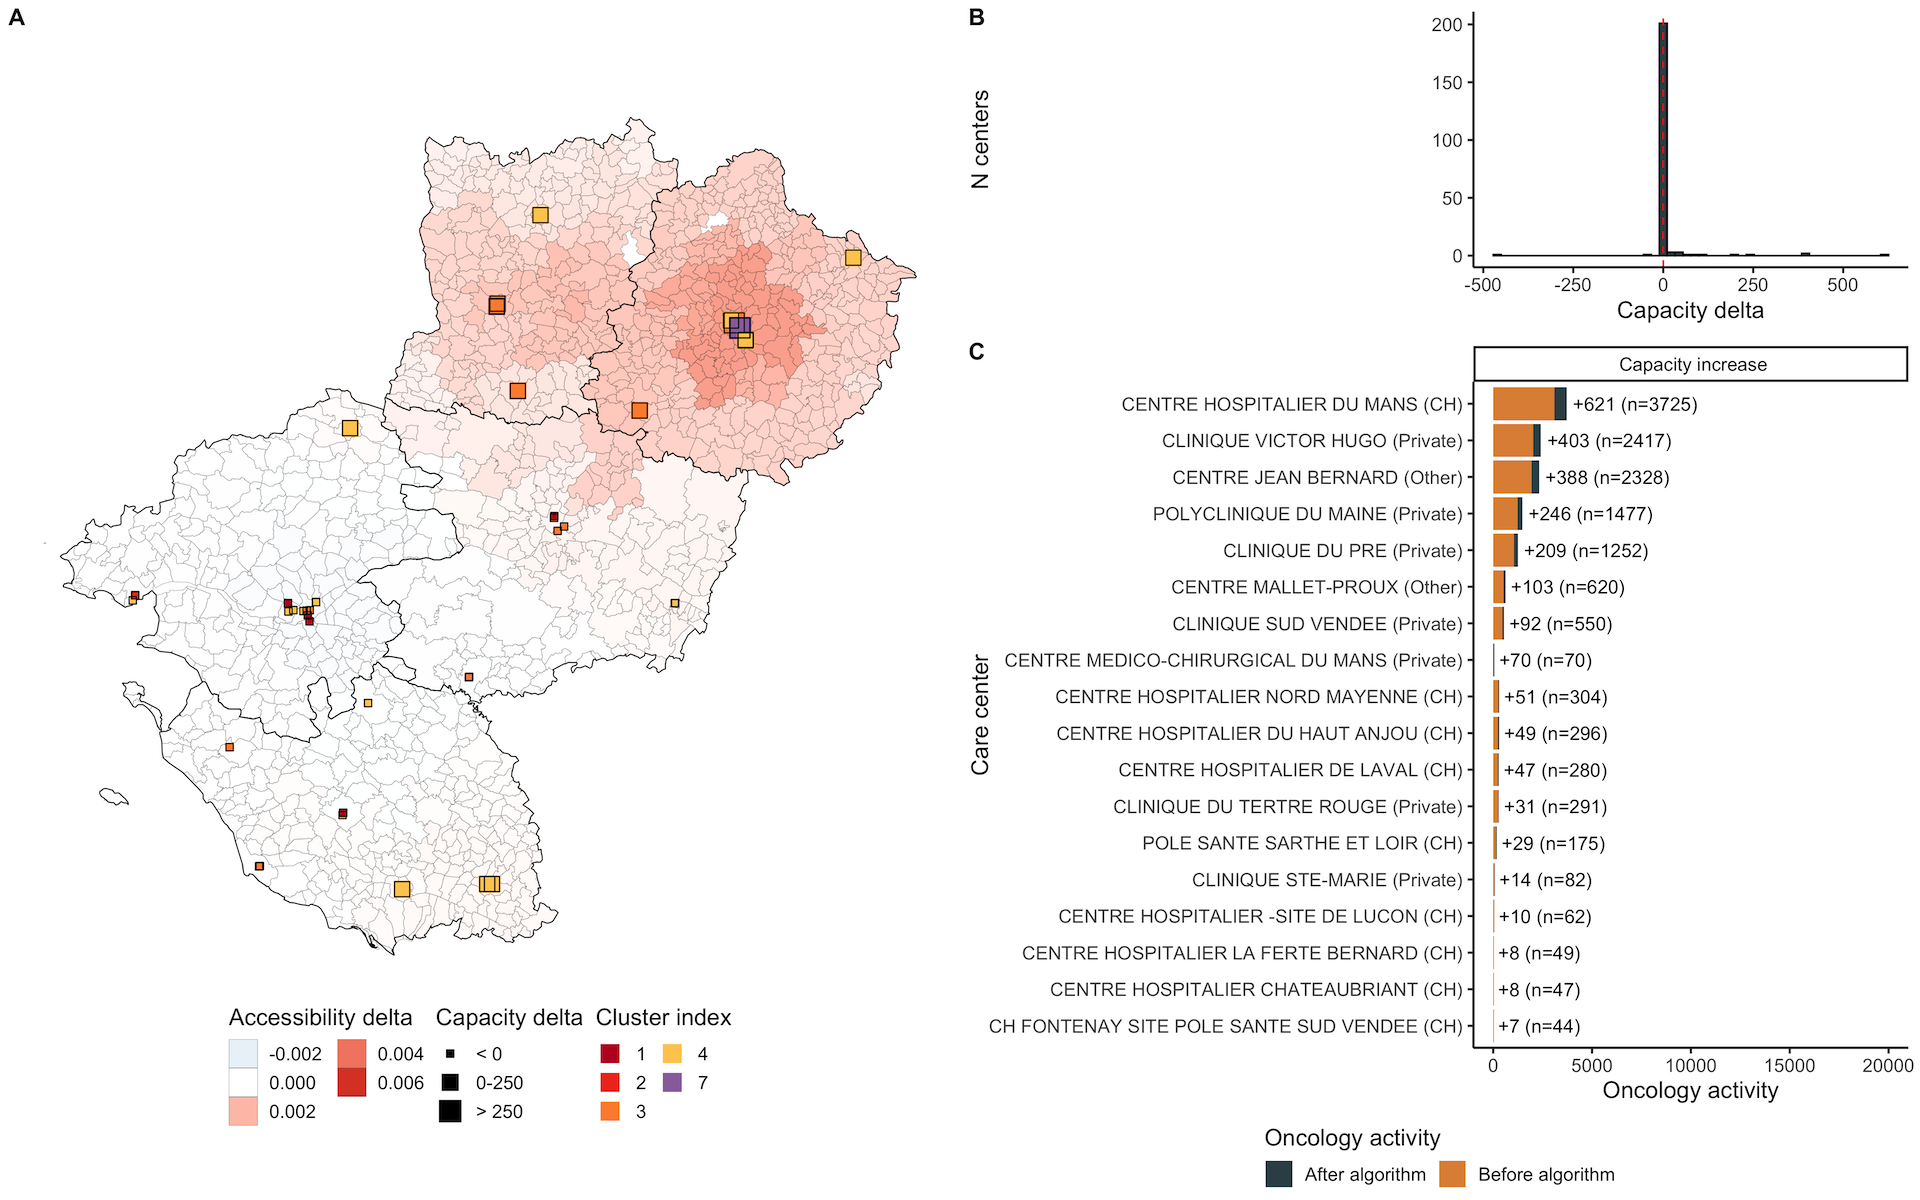
\includegraphics[width=\textwidth]{images/camion/optim_region/optim_Pays-de-la-Loire.png}
    \centering
    \caption{
        Optimization results in Pays-de-la-Loire. Additional activity was 1,890. 18 centers grew and 2 decreased. Median accessibility before optimization was 0.0118 and 0.0121 after, corresponding to a 2.4\% increase. Accessibility grew near La Roche sur Yon, Angers and Le Mans.
    }
\end{figure}

\subsection*{Occitanie}

\begin{figure}[h]
    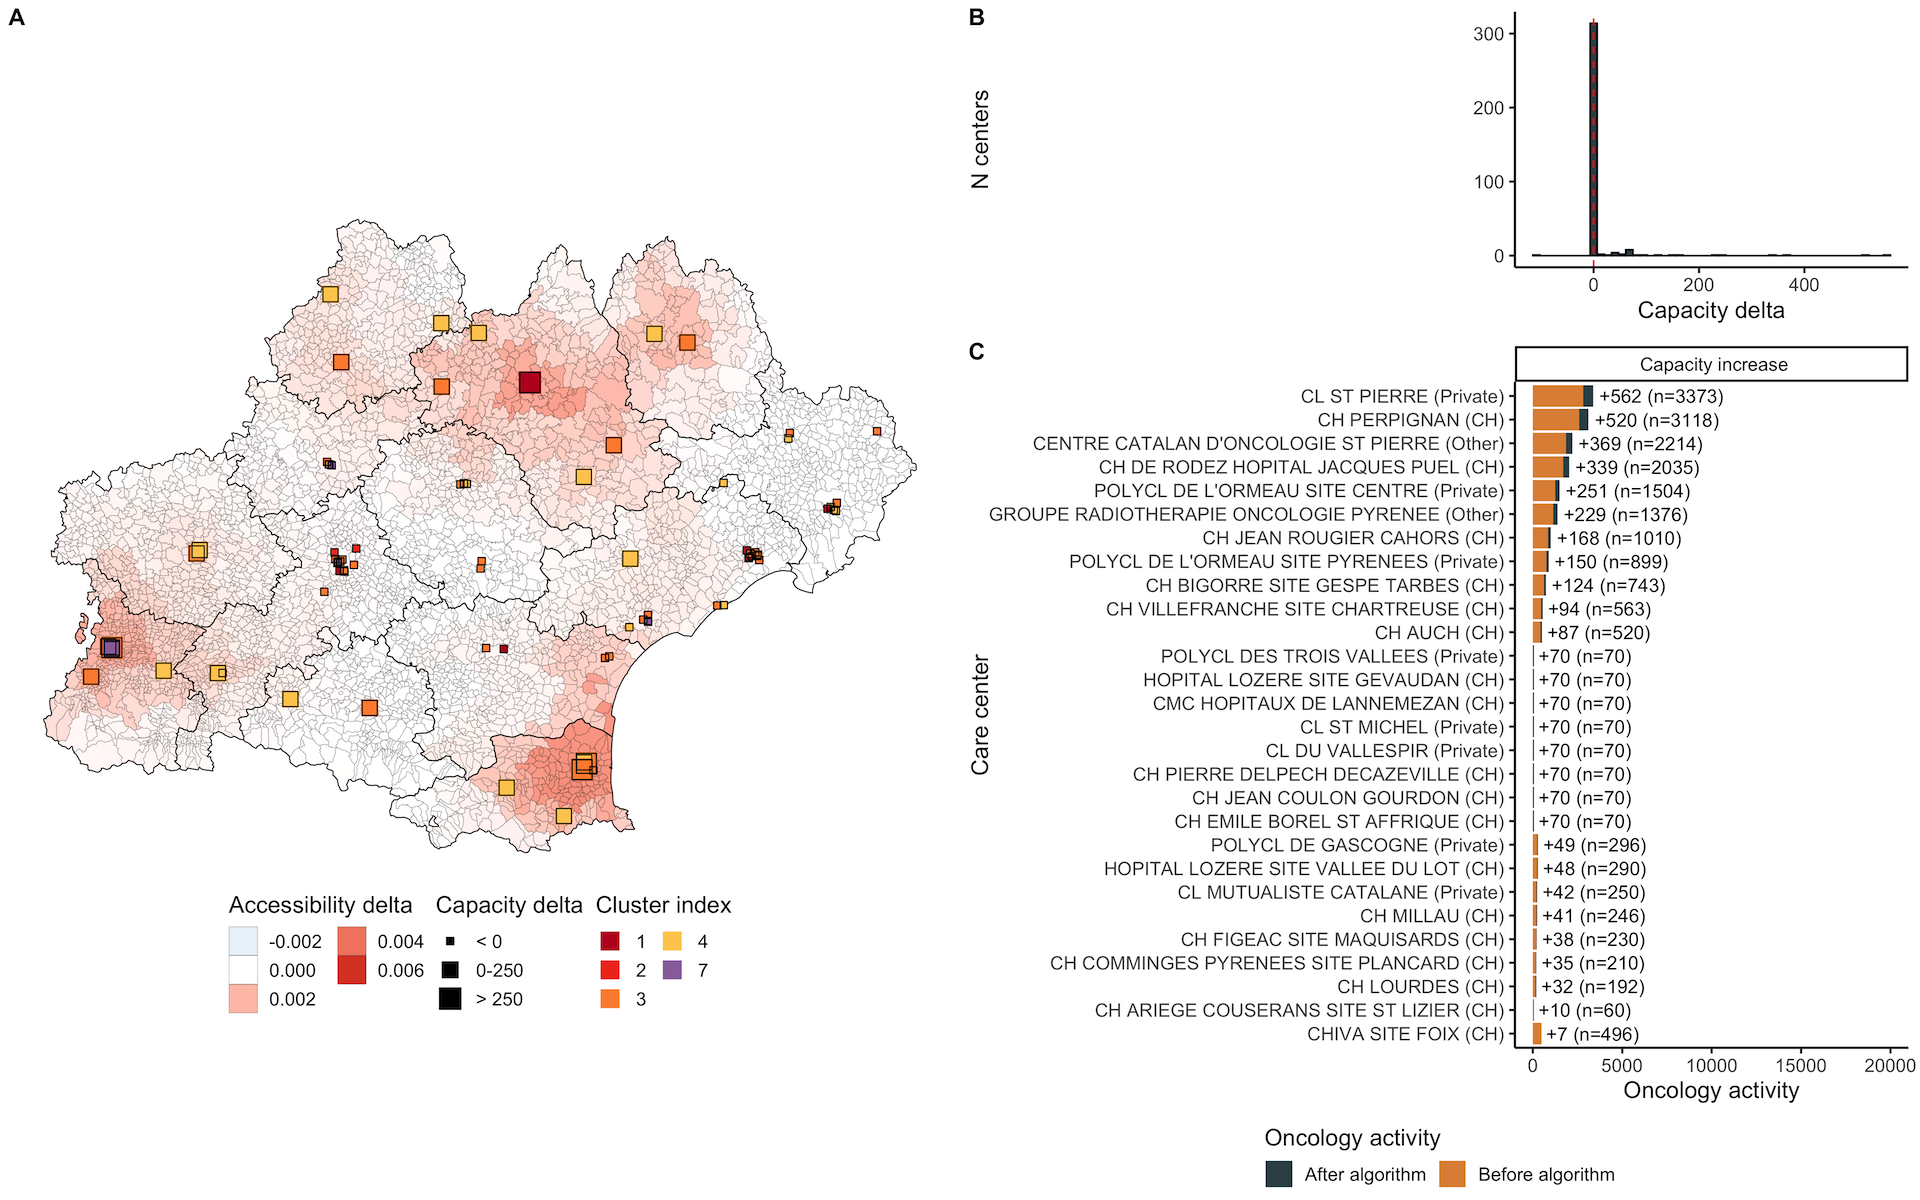
\includegraphics[width=\textwidth]{images/camion/optim_region/optim_Occitanie.png}
    \centering
    \caption{
        Optimization results in Occitanie. Additional activity was 3,652. 28 centers grew and 1 decreased. Median accessibility before optimization was 0.0087 and 0.0091 after, corresponding to a 4.7\% increase. Accessibility grew around Perpignan, Rodez, Mende and Tarbes.
    }
\end{figure}

\subsection*{Nouvelle-Aquitaine}

\begin{figure}[h]
    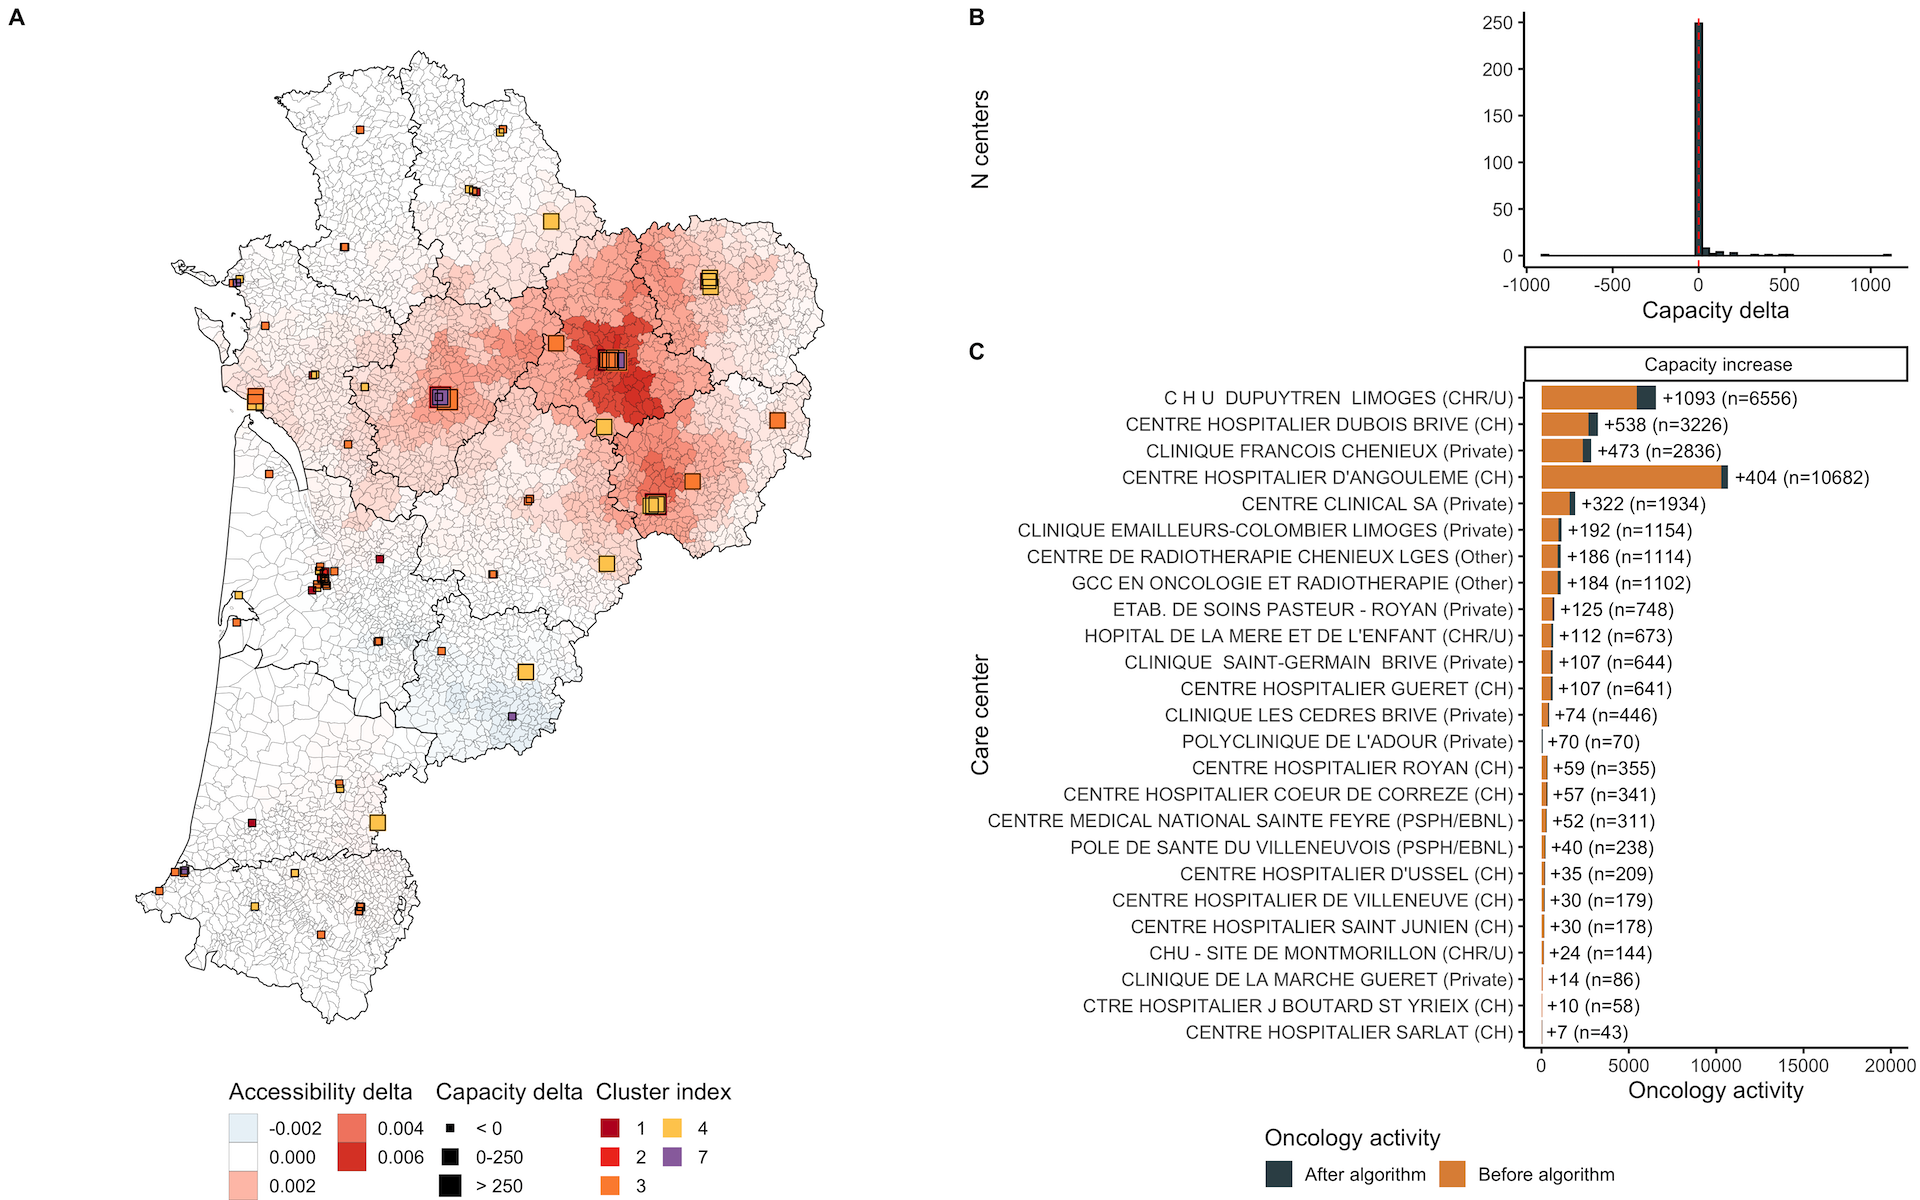
\includegraphics[width=\textwidth]{images/camion/optim_region/optim_Nouvelle-Aquitaine.png}
    \centering
    \caption{
        Optimization results in Nouvelle-Aquitaine. Additional activity was 3,445. 25 centers grew and 1 decreased. Median accessibility before optimization was 0.0117 and 0.0119 after, corresponding to a 1.5\% increase. Accessibility grew around Limoges, Angouleme, and Brives-la-Gaillarde.
    }
\end{figure}

\subsection*{Normandie}

\begin{figure}[h]
    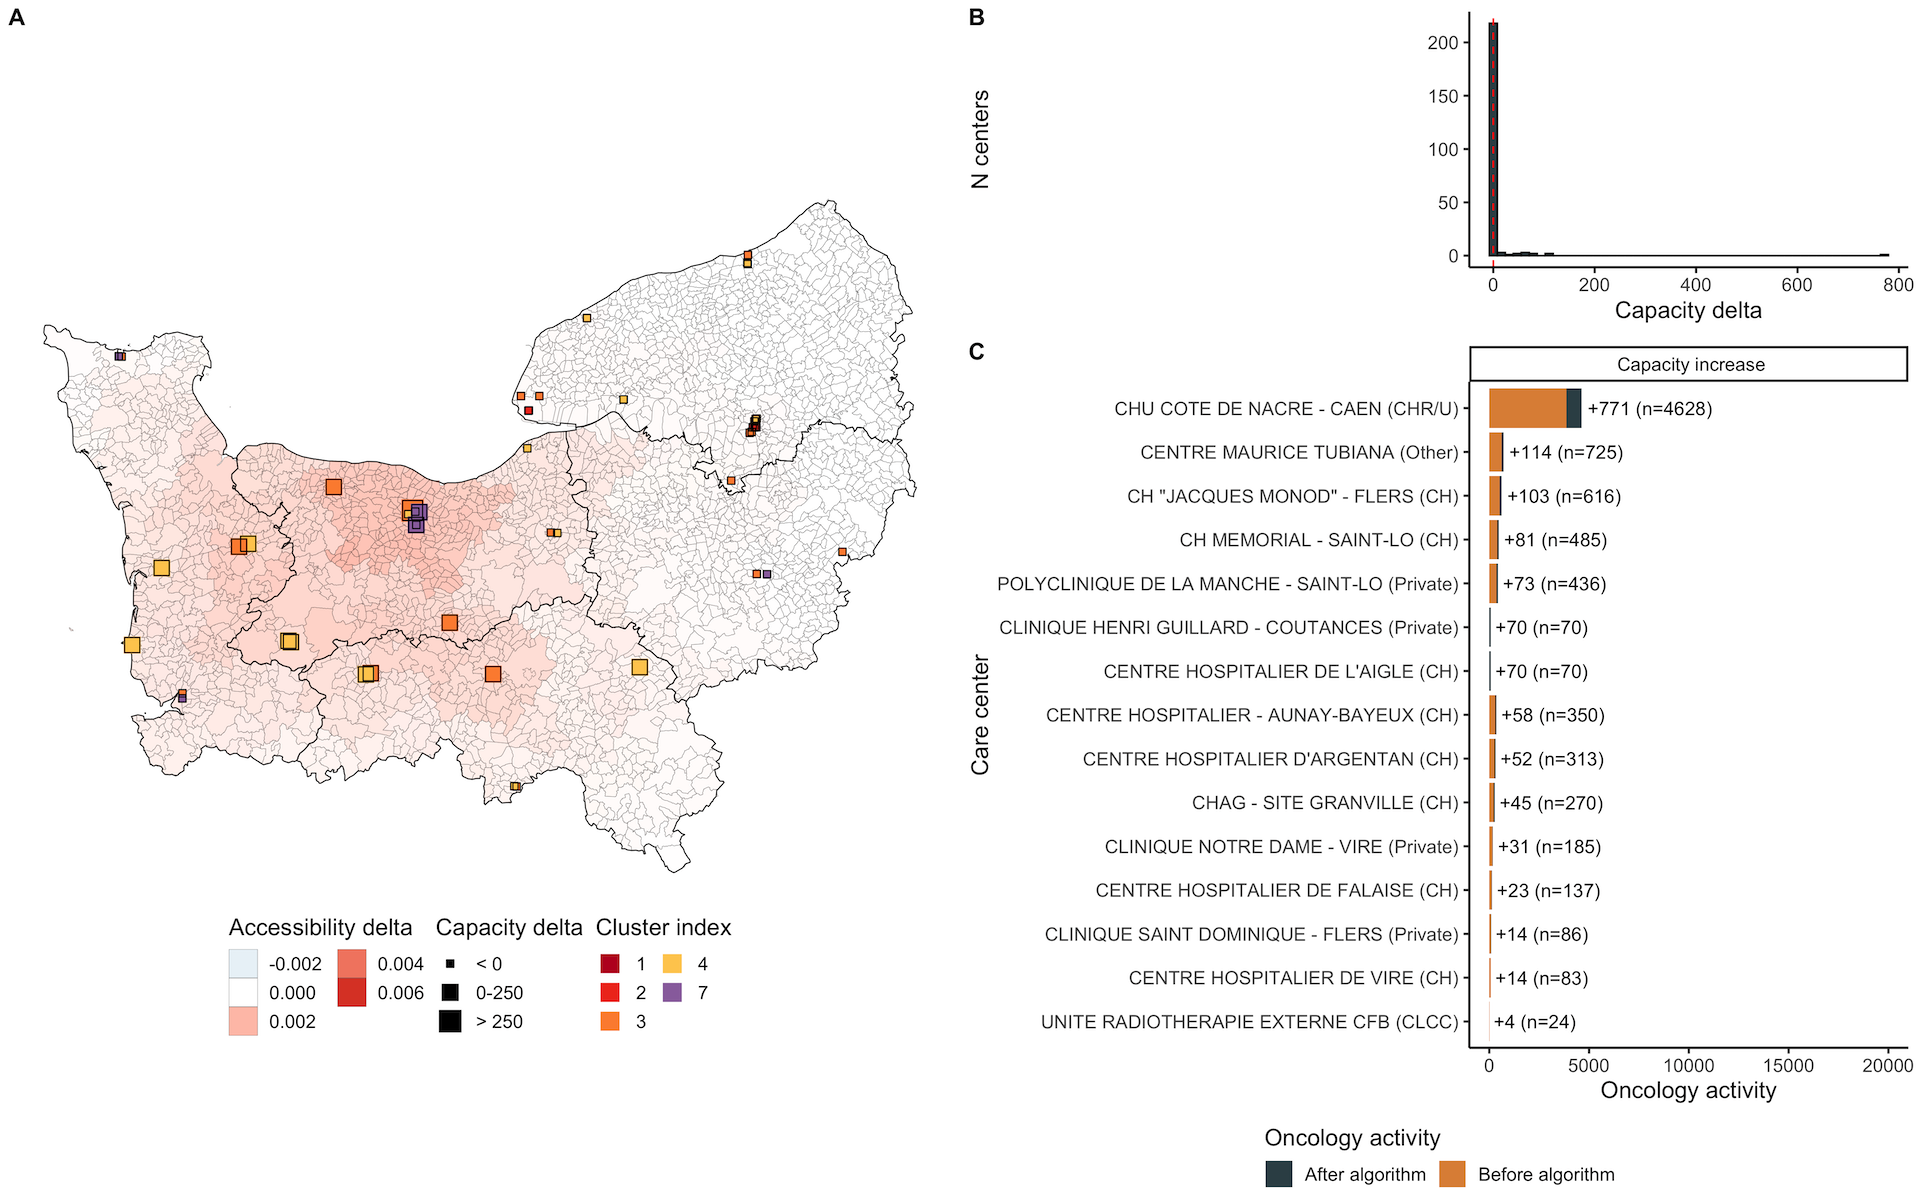
\includegraphics[width=\textwidth]{images/camion/optim_region/optim_Normandie.png}
    \centering
    \caption{
        Optimization results in Normandie. Additional activity was 1,523. 15 centers grew and 0 decreased. Median accessibility before optimization was 0.0105 and 0.0106 after, corresponding to a 1\% increase. Accessibility grew near Caen, Argentan, and St-Lo.
    }
\end{figure}

\subsection*{Île-de-France}

\begin{figure}[h]
    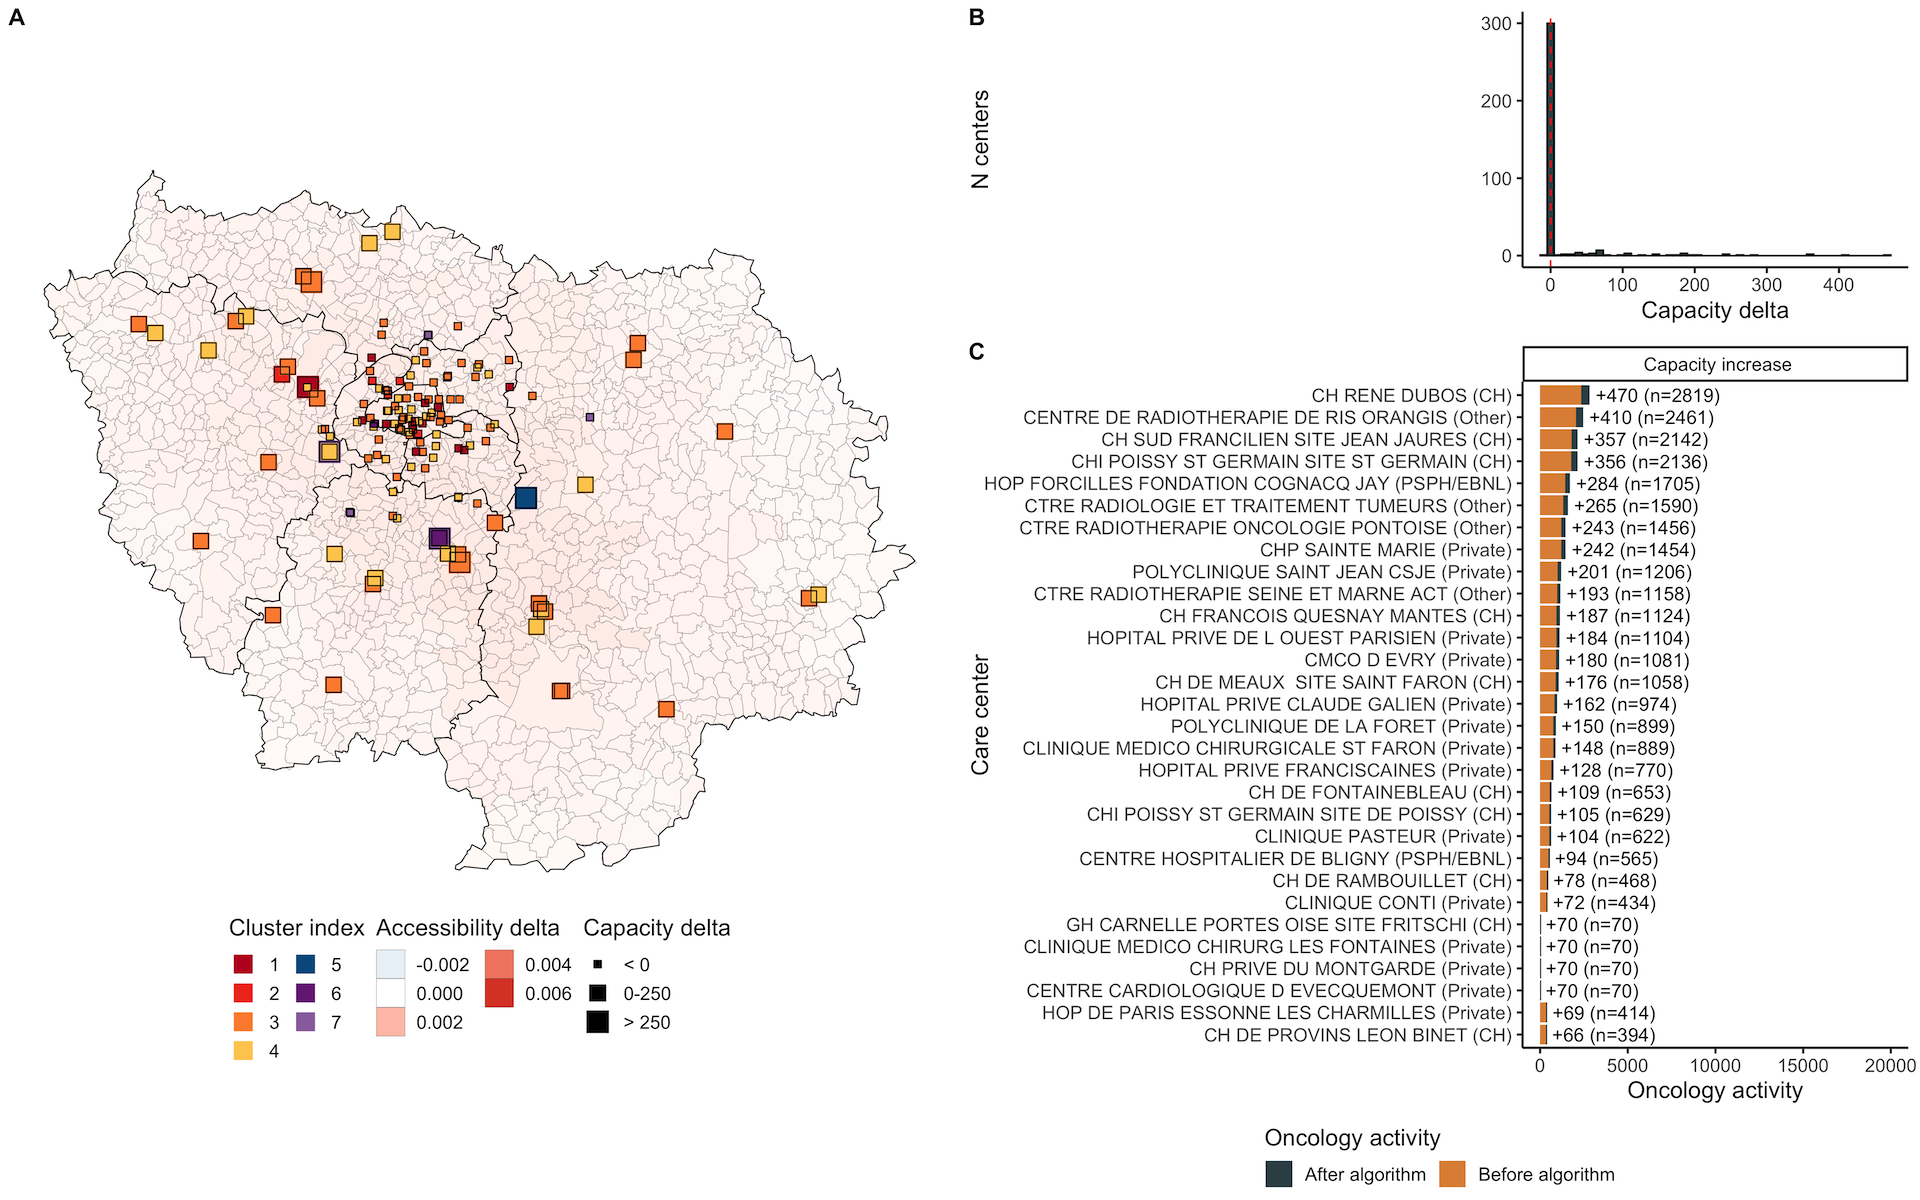
\includegraphics[width=\textwidth]{images/camion/optim_region/optim_Ile-de-France.png}
    \centering
    \caption{
        Optimization results in Ile-de-France. Additional activity was 5,826. 44 centers grew and 1 decreased. Median accessibility before optimization was 0.0088 and 0.0089 after, corresponding to a 1.3\% increase. Accessibility grew around Mantes-la-Jolie, Rambouillet, Melun, and Evry.
    }
\end{figure}

\subsection*{Hauts-de-France}

\begin{figure}[h]
    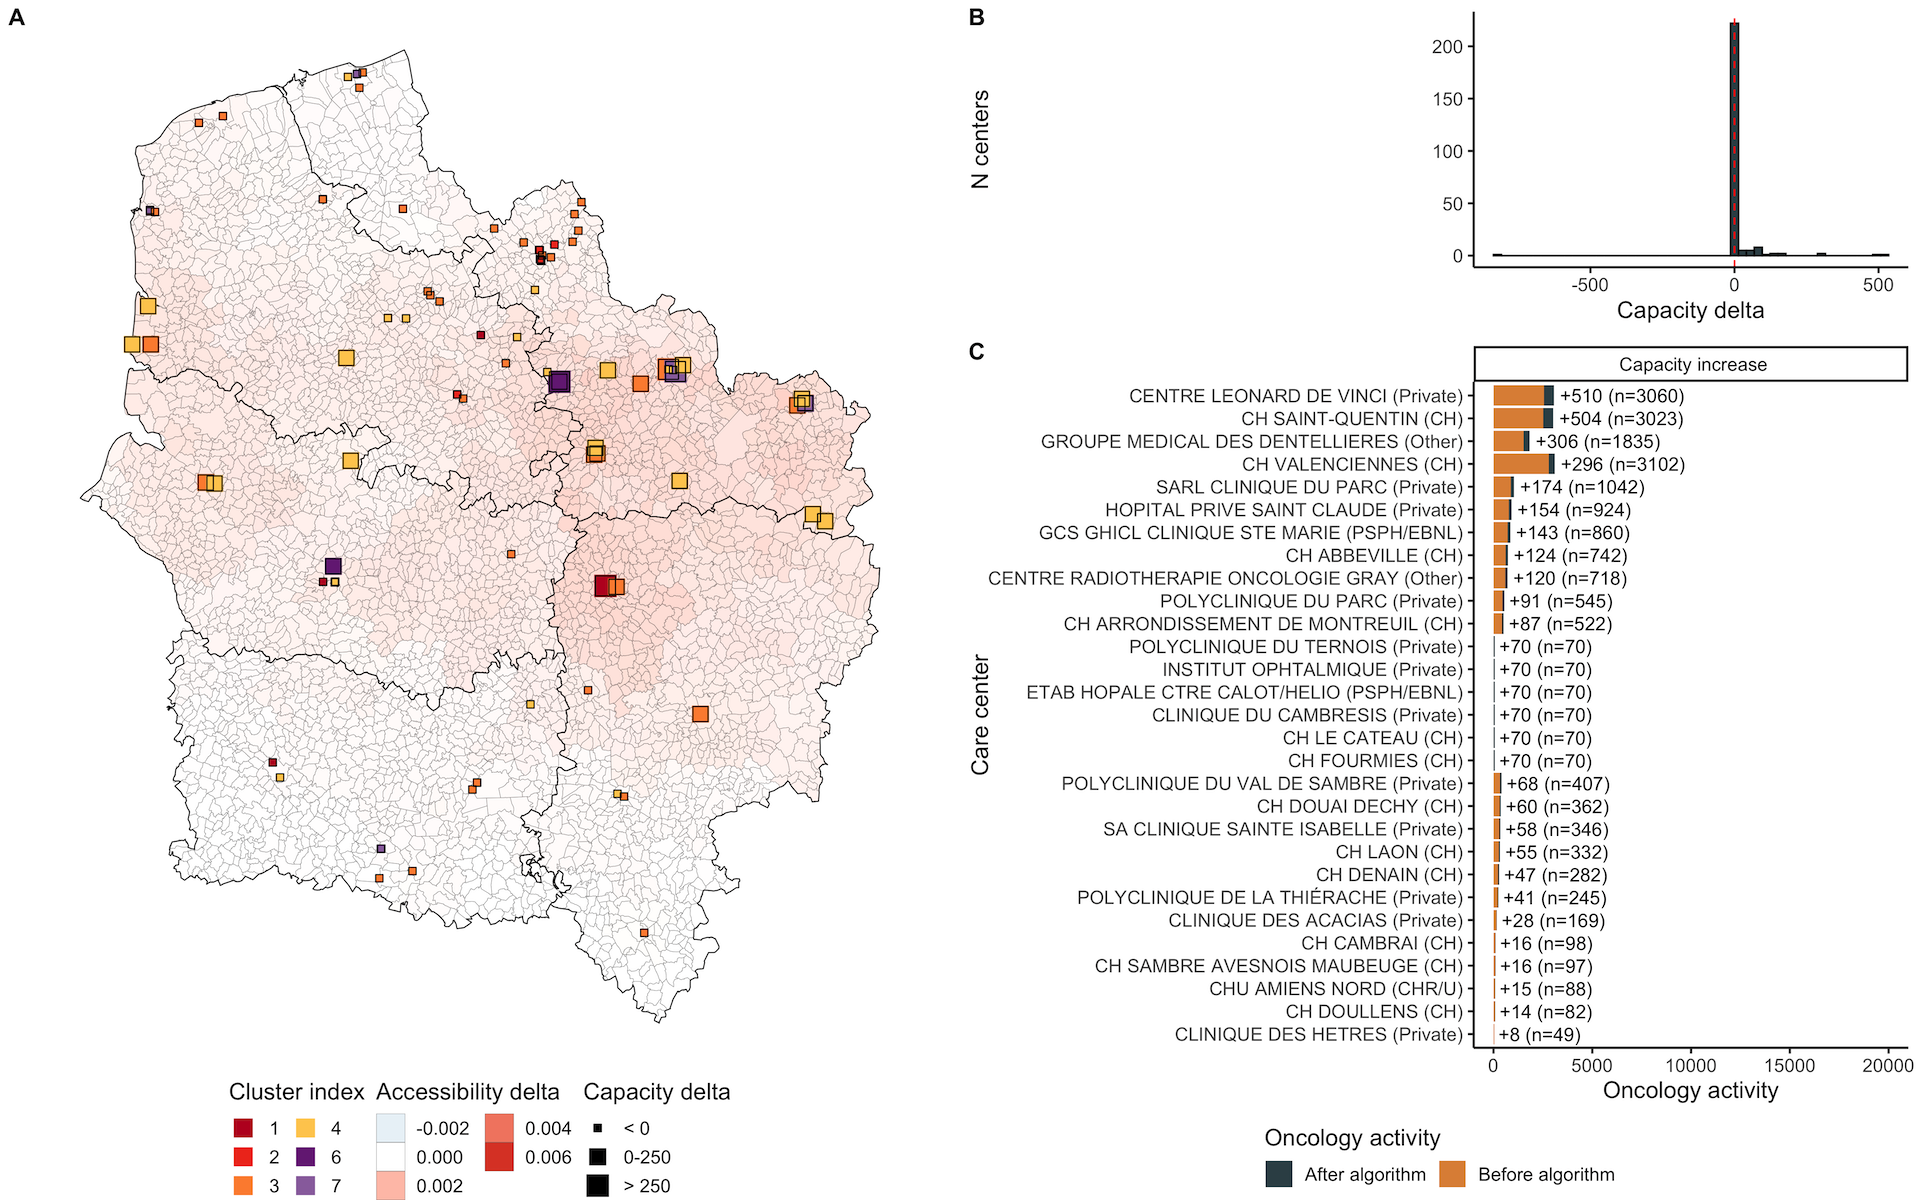
\includegraphics[width=\textwidth]{images/camion/optim_region/optim_Hauts-de-France.png}
    \centering
    \caption{
        Optimization results in Hauts-de-France. Additional activity was 2,520. 29 centers grew and 1 decreased. Median accessibility before optimization was 0.01 and 0.0102 after, corresponding to a 2.1\% increase. Accessibility grew around St-Quentin and Valenciennes.
    }
\end{figure}

\subsection*{Grand Est}

\begin{figure}[h]
    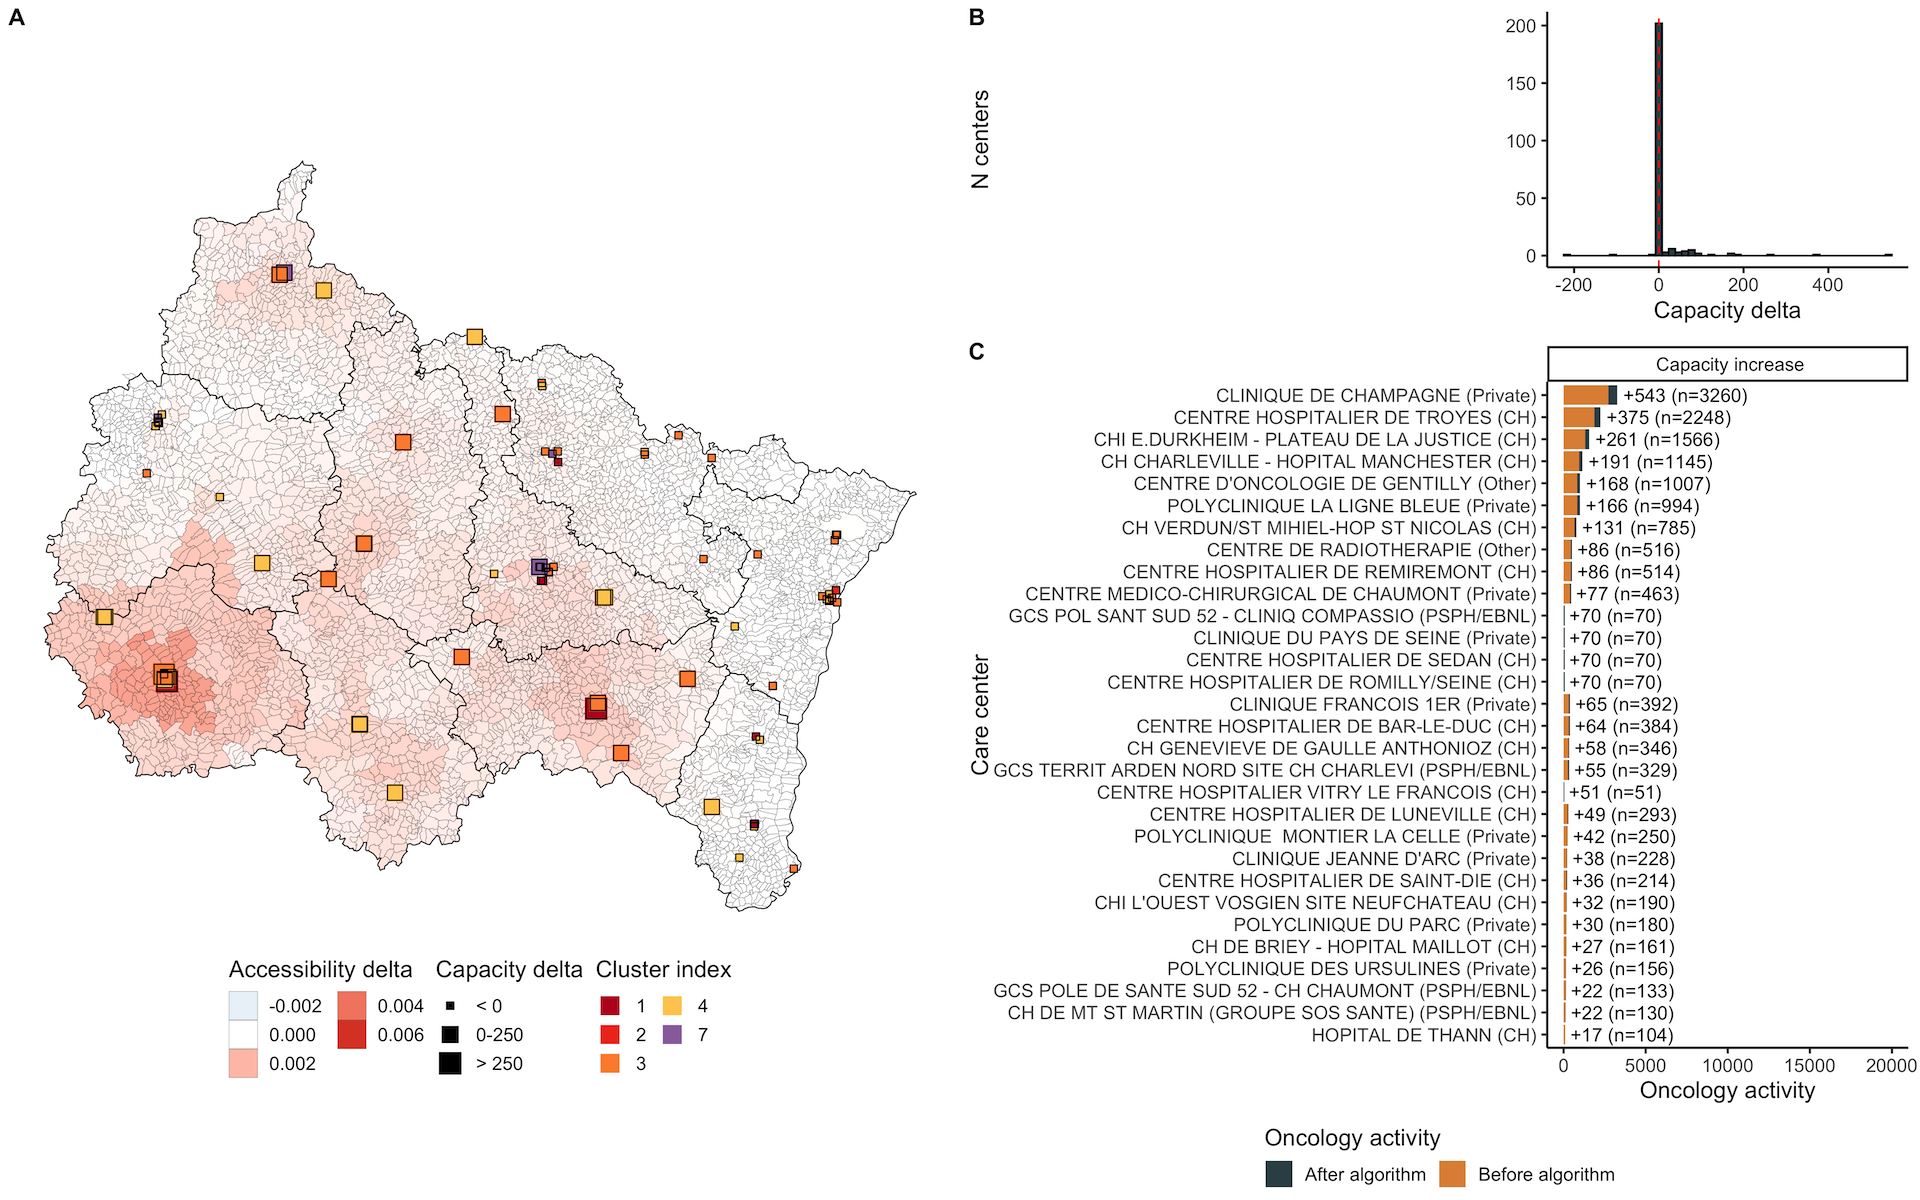
\includegraphics[width=\textwidth]{images/camion/optim_region/optim_Grand-Est.png}
    \centering
    \caption{
        Optimization results in Grand-Est. Additional activity was 2,663. 31 centers grew and 4 decreased. Median accessibility before optimization was 0.0096 and 0.0099 after, corresponding to a 3\% increase. Accessibility grew around Troyes and Epinal.
    }
\end{figure}

\subsection*{Centre-Val de Loire}

\begin{figure}[h]
    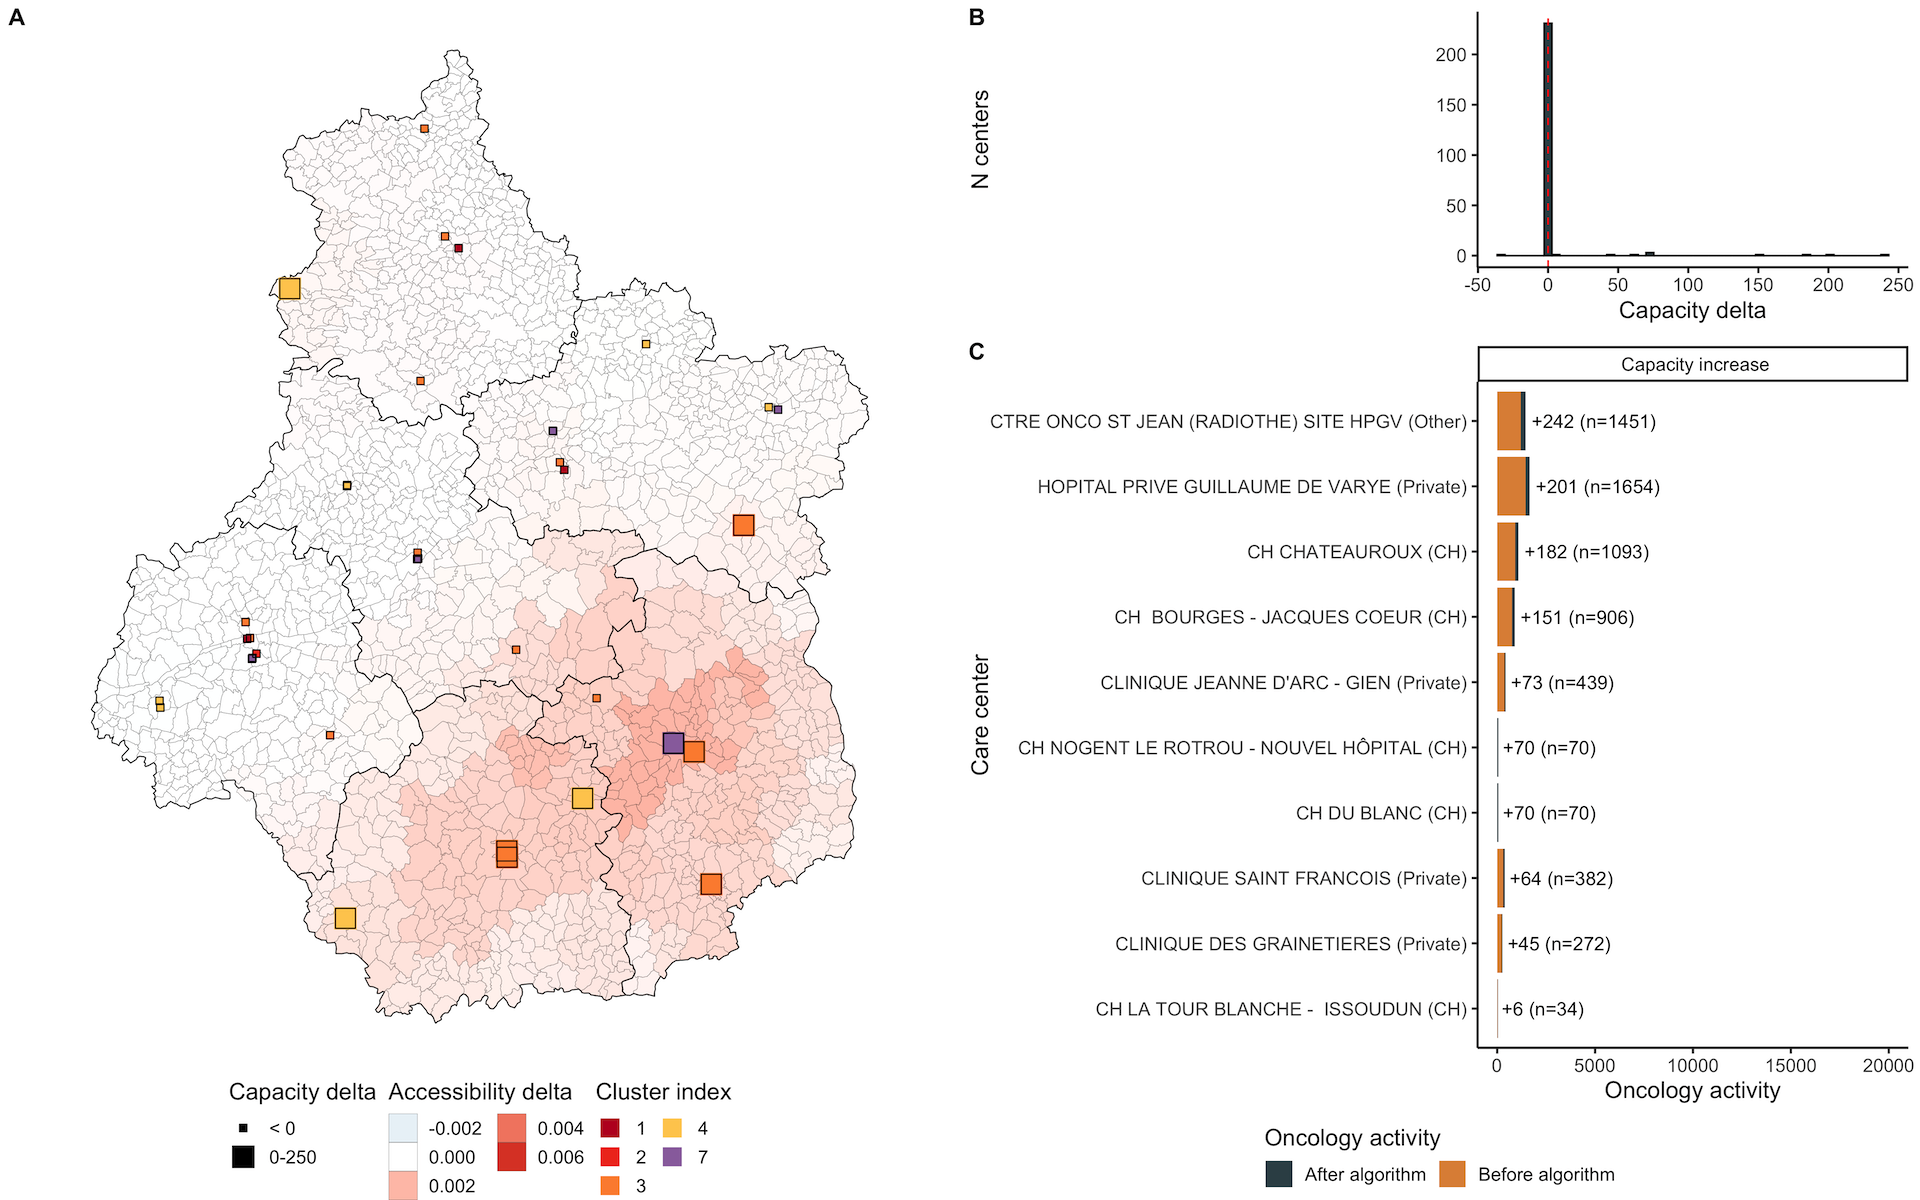
\includegraphics[width=\textwidth]{images/camion/optim_region/optim_Centre-Val-de-Loire.png}
    \centering
    \caption{
        Optimization results in Centre-Val-de-Loire. Additional activity was 1,072. 10 centers grew and 1 decreased. Median accessibility before optimization was 0.0099 and 0.0102 after, corresponding to a 2.9\% increase. Accessibility grew around Tours, Blois, Bourges and Chateauroux.
    }
\end{figure}

\subsection*{Bretagne}

\begin{figure}[h]
    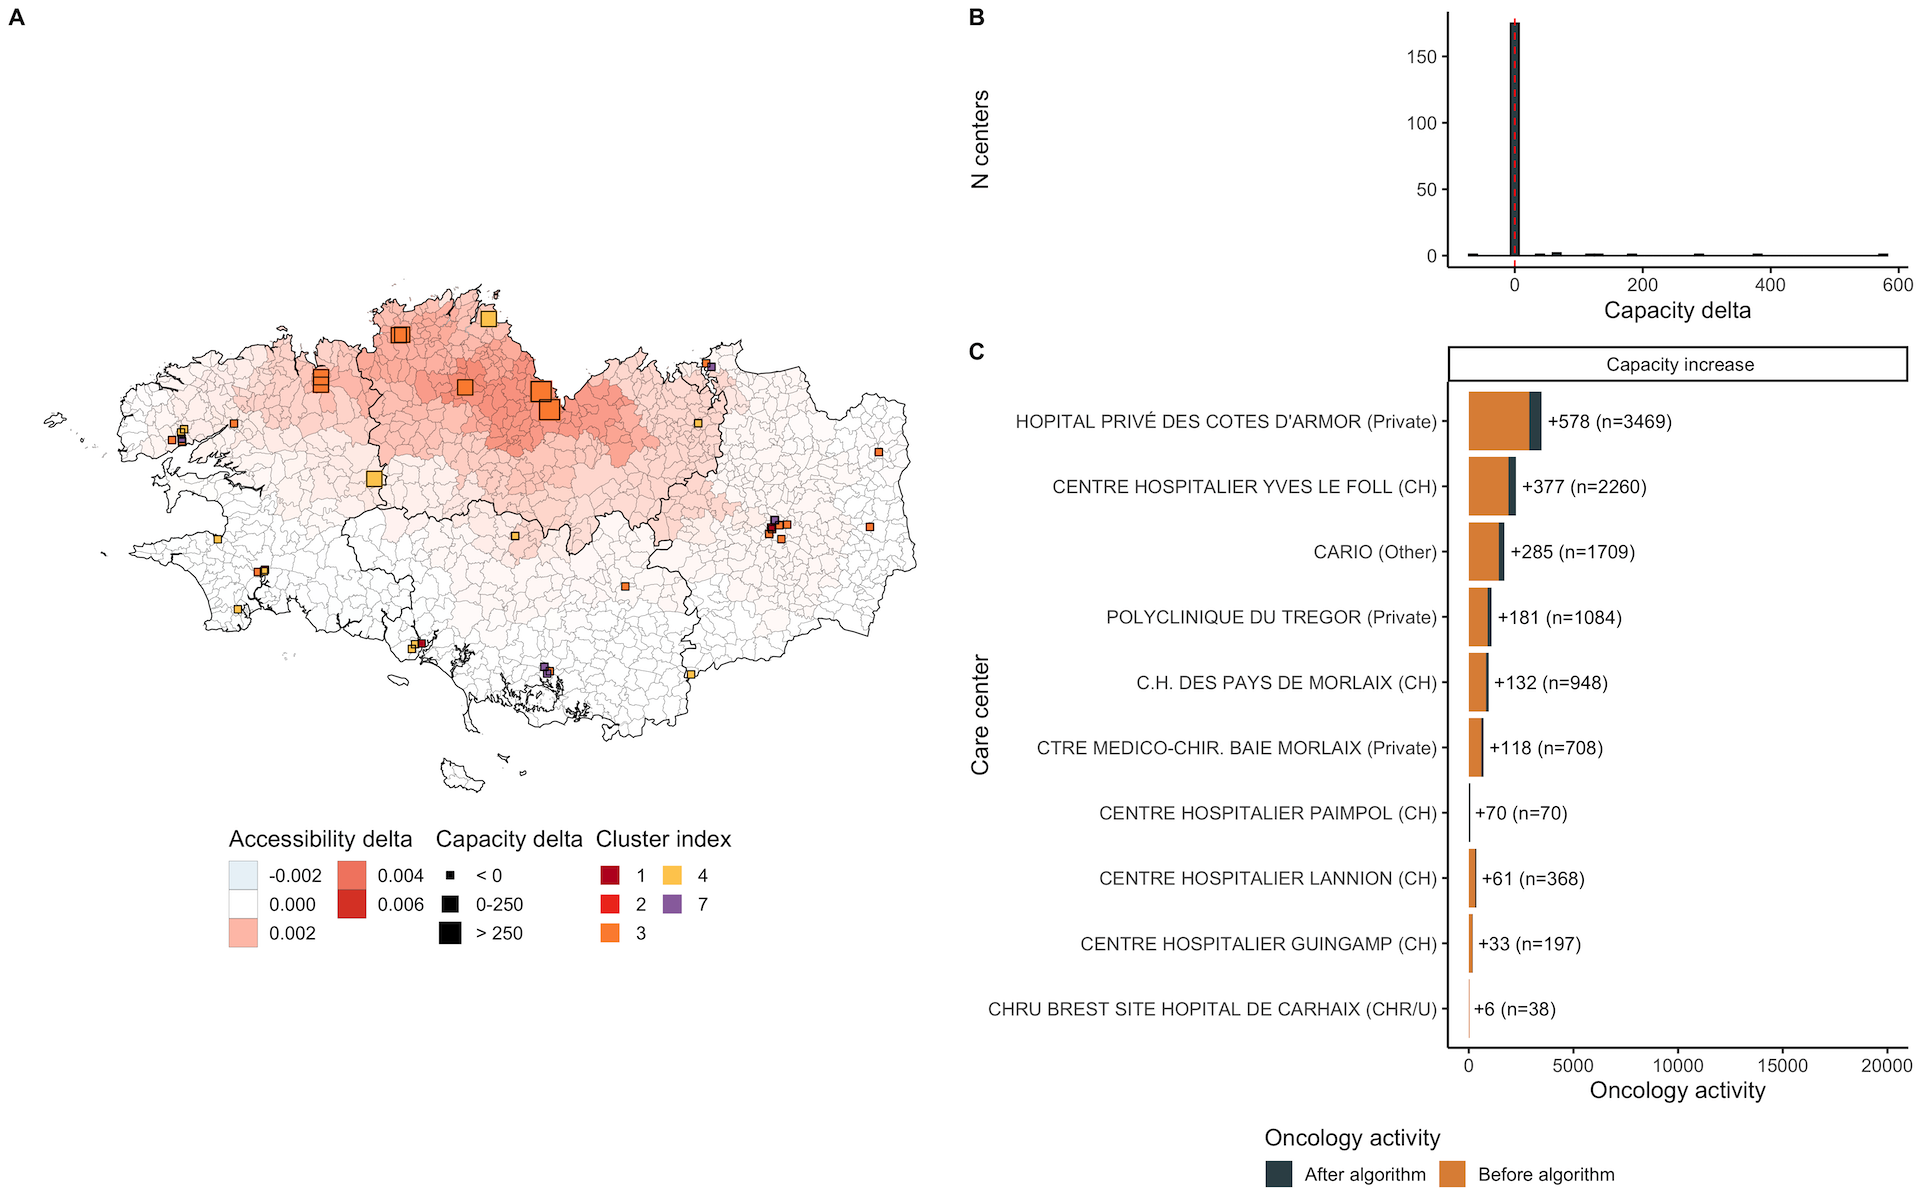
\includegraphics[width=\textwidth]{images/camion/optim_region/optim_Bretagne.png}
    \centering
    \caption{
        Optimization results in Bretagne. Additional activity was 1,773. 10 centers grew and 2 decreased. Median accessibility before optimization was 0.0131 and 0.0134 after, corresponding to a 2.4\% increase. Accessibility grew around St-Brieuc and Quimper.
    }
\end{figure}

\subsection*{Bourgogne-Franche-Comté}

\begin{figure}[h]
    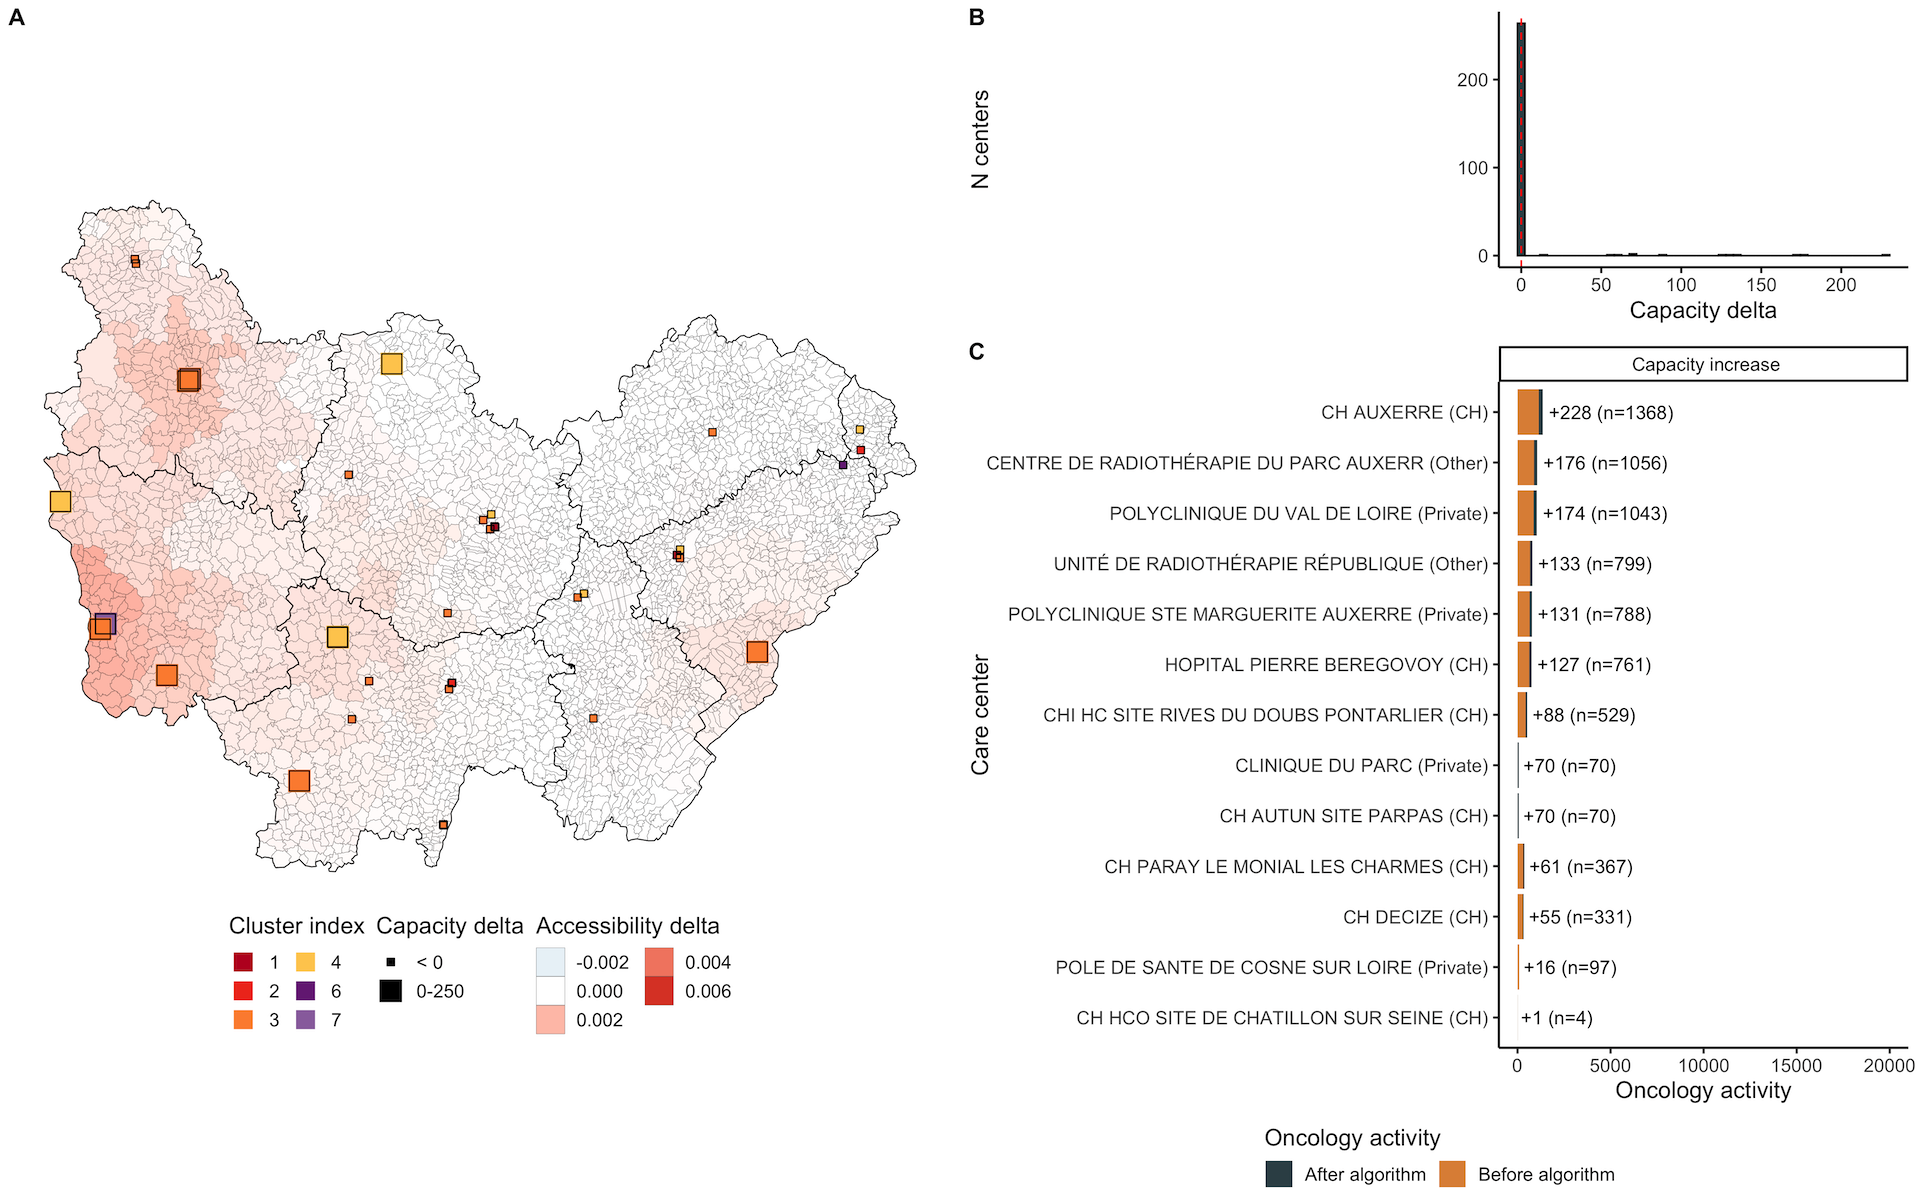
\includegraphics[width=\textwidth]{images/camion/optim_region/optim_Bourgogne-Franche-Comte.png}
    \centering
    \caption{
        Optimization results in Bourgogne-Franche-Comté. Additional activity was 1,330. 13 centers grew and 0 decreased. Median accessibility before optimization was 0.0096 and 0.0098 after, corresponding to a 1.9\% in-crease. Accessibility grew around Nevers, Belfort, Vesoul and Auxerre.
    }
\end{figure}

\subsection*{Auvergne-Rhône-Alpes}

\begin{figure}[h]
    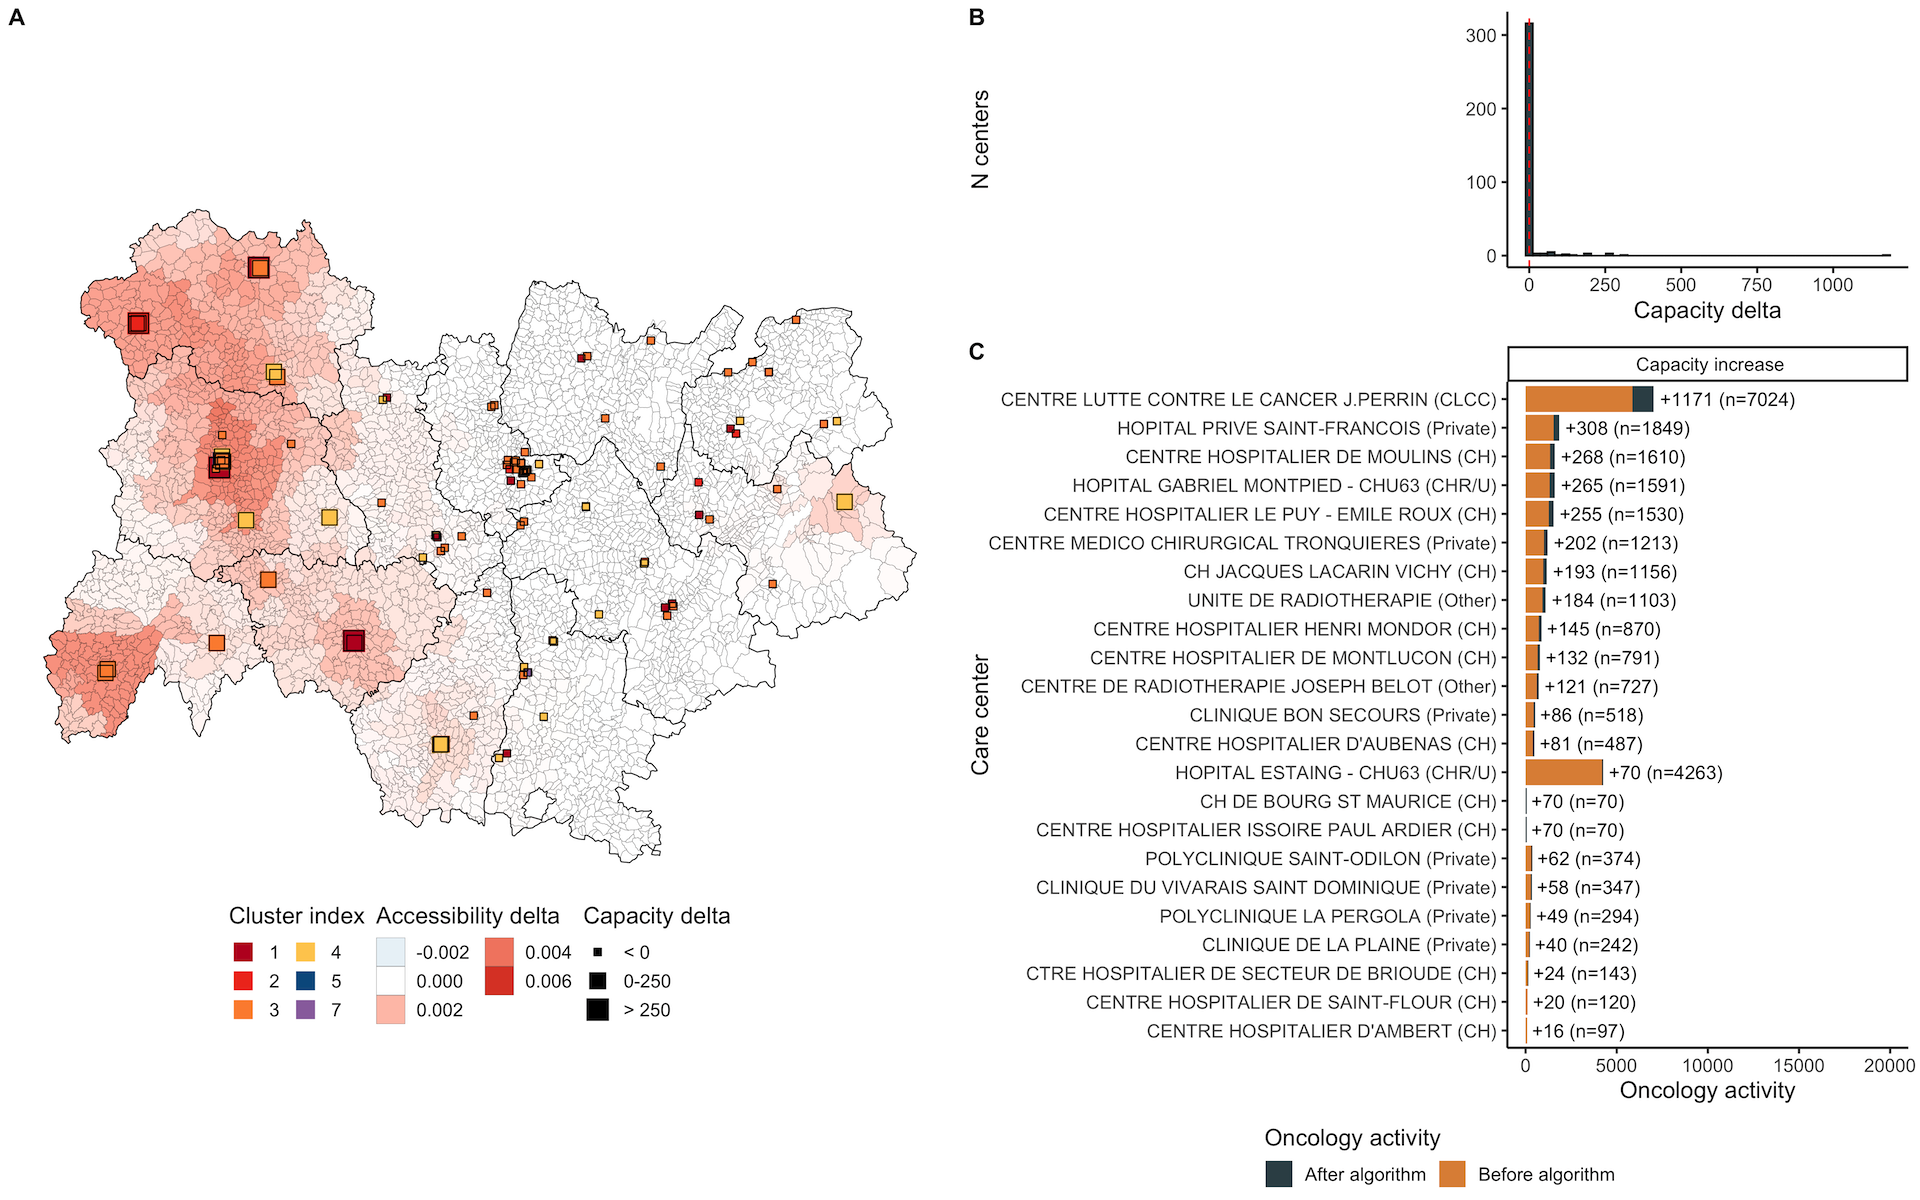
\includegraphics[width=\textwidth]{images/camion/optim_region/optim_Auvergne-Rhone-Alpes.png}
    \centering
    \caption{
        Optimization results in Auvergne-Rhone-Alpes. Additional activity was 3,883. 23 centers grew and 2 de-creased. Median accessibility before optimization was 0.0092 and 0.0095 after, corresponding to a 3.2\% in-crease. Accessibility grew around Moulins, Montluçon, Le Puy en Velay, Clermont-Ferrand and Aurillac.
    }
\end{figure}

\section{Web application}

We developed a web application that allows the users to run the optimization algorithm in any region with the parameters they want. The application displays accessibility results and optimization outcomes on an interactive map with additional plots. The user can browse the list of care centers by cluster and the list of municipalities with their accessibility scores.

\section{Open source code}

We open sourced the code for accessibility computation and \ac{camion} algorithm.
The code is available in the following Github repository: \url{https://github.com/ericdaat/CAMION}.

We applied our method to Health Facilities in New York City. We used datasets downloaded from NYC Open Data website, which lists free public data from New York City agencies and other partners. We downloaded the Zip Codes boundaries and census statistics in New York City, provided by the Department of Information Technology and Telecommunications. We retrieved the list of health facilities in the New York State, as well as their certifications for services and beds. Both datasets were provided by the New York State Department of Health. We only kept the health facilities located in New York City, with Medical / Surgical beds. Every hospital has Latitude / Longitude coordinates. We used Zip Codes polygons centroids as reference point to compute the travel between Zip Codes and hospitals. We used the Zip code population as $P_i$, to encode the demand variable. The supply variable $S_u$ was the number of Medical / Surgery bed for each Health Facility $u$. We used the geodesic (straight) distance between health facilities coordinates, and Zip Code centroid coordinates as distance matrix.

Download the datasets here:

\begin{itemize}
    \item \href{https://data.beta.nyc/dataset/nyc-zip-code-tabulation-areas/resource/894e9162-871c-4552-a09c-c6915d8783fb}{Zip Codes boundaries and census statistics in New York City}
    \item \href{https://health.data.ny.gov/Health/Health-Facility-General-Information/vn5v-hh5r}{List of health facilities in NY State}
    \item \href{https://health.data.ny.gov/Health/Health-Facility-Certification-Information/2g9y-7kqm}{Health facilities certifications for services and beds}
\end{itemize}

\begin{figure}[h]
    \includegraphics[width=\textwidth]{images/camion-ny/fig1.png}
    \centering
    \caption{
        Health facilities with Medical / Surgery beds in New York City. We included 55 facilities with a total of 13,443 beds. Map (A) shows the geographical location of the facilities, colored by county, and sized by number of beds. The distribution of the number of beds is shown on (B). The top 30 facilities with the highest number of beds are listed on (C) and colored by county. The largest facilities are in New-York County.
    }
    \label{fig:camion-ny-beds}
\end{figure}

\begin{lstlisting}[language=Python, caption=Compute accessibility score with \ac{e2sfca}]
from camion.fca import E2SFCA

# Declare variables
P_i = np.random.rand(100)
S_j = np.random.rand(10)
D_ij = np.random.randint(low=1, high=100, size=(100, 10))

# Init E2SFCA algorithm
e2sfca = E2SFCA(
    S_j=S_j,   # Facilities
    P_i=P_i,   # Population locations
    D_ij=D_ij  # Travel impedance
)

# Choose weights for travel impedance
weights = [(30, 1), (60, 0.42), (90, 0.09)]

# Compute accessibility scores
A_i = e2sfca.compute_accessibility_score(weights)
\end{lstlisting}

\begin{figure}[h]
    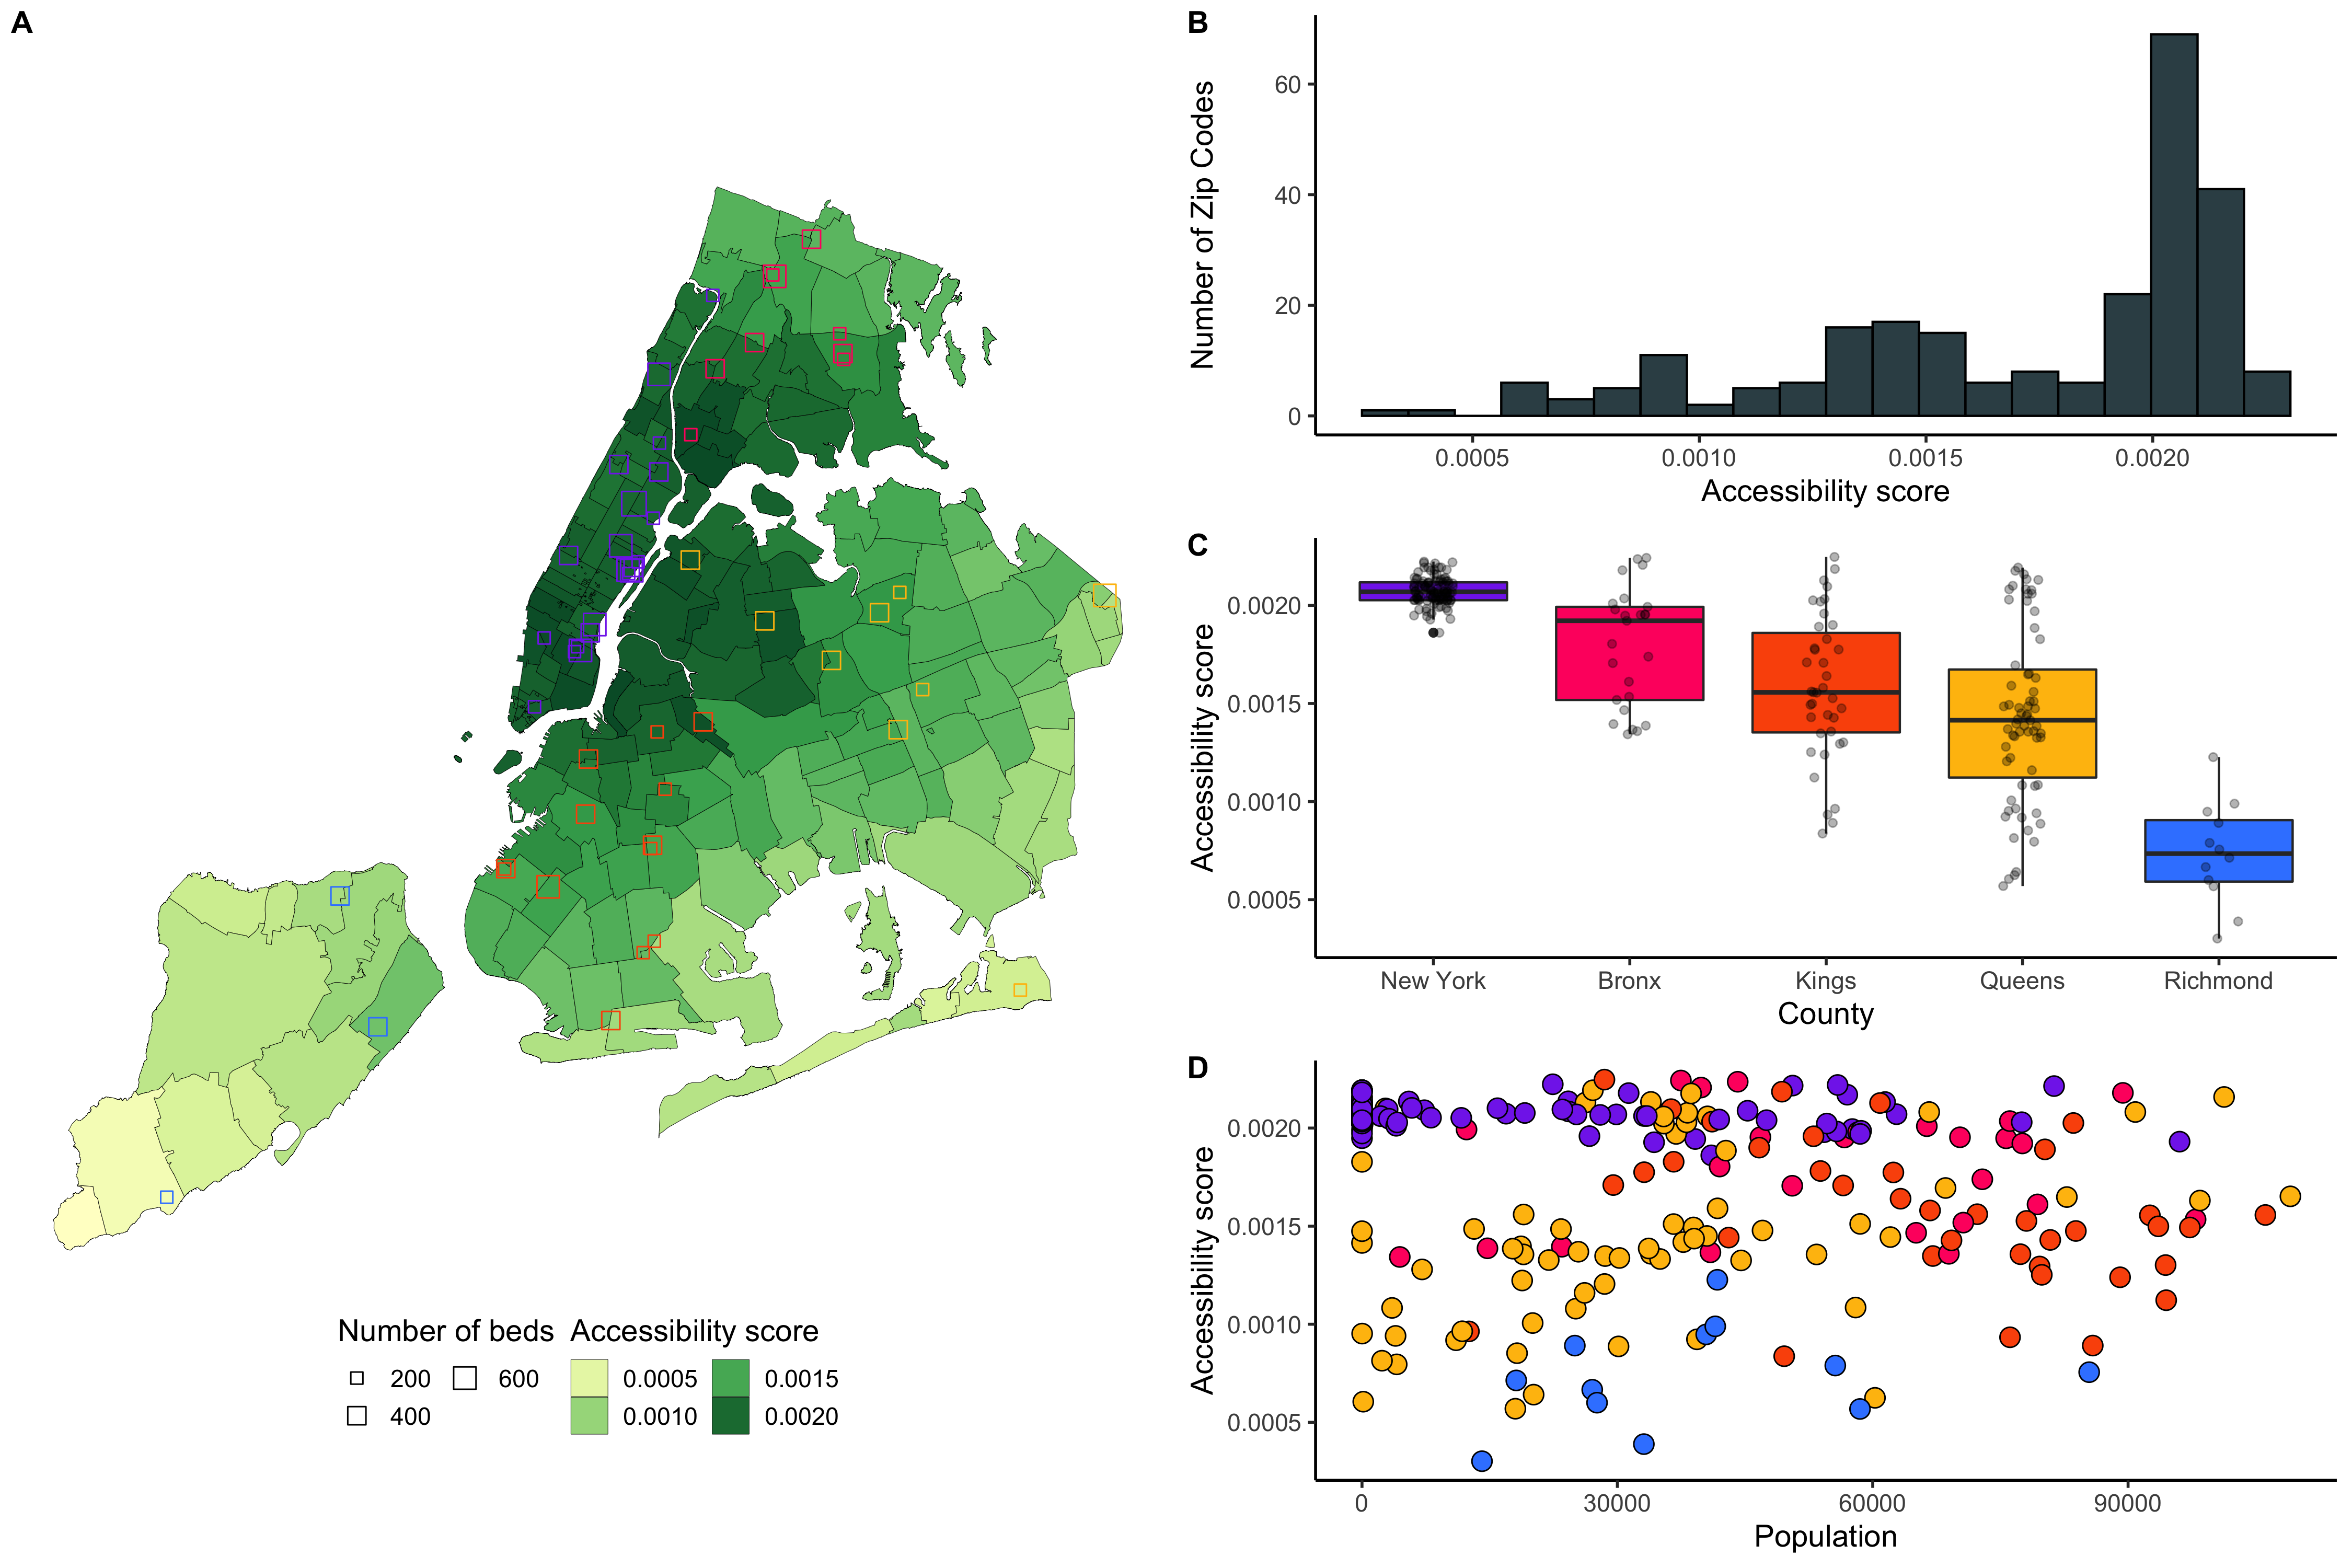
\includegraphics[width=\textwidth]{images/camion-ny/fig2.png}
    \centering
    \caption{
        Accessibility to Medical / Surgery beds in New York City. Accessibility score was computed with the Enhanced Two Step Floating Catchment Area method, with a 45 km maximum catchment area. The geographical distribution of the accessibility score is shown on map (A). Zip codes are colored by accessibility score. Facilities are sized by number of beds and colored by county. The overall accessibility distribution is shown on (B). New-York County has the highest accessibility distribution where Richmond has the lowest (C). Accessibility seems to be higher in dense areas but there is no significant correlation between accessibility and population (D).
    }
    \label{fig:camion-ny-accessibility}
\end{figure}

\begin{lstlisting}[language=Python, caption=Optimize accessibility with \acs{camion}]
from camion.optimization import RegularOptimizer, MaxiMinOptimizer

# Define optimization parameters
budget = 1000
growth_percentage = 0.3

# Init regular optimizer
regular_optimizer = RegularOptimizer()

# Init maximin optimizer
maximin_optimizer = MaxiMinOptimizer()

# Run optimization with the optimization parameters
S_j_new_regular = regular_optimizer.run_optimization(
    S_j, P_i, W_ij,
    budget, growth_percentage
)

S_j_new_maximin = maximin_optimizer.run_optimization(
    S_j, P_i, W_ij,
    budget, growth_percentage
)
\end{lstlisting}

\begin{figure}[h]
    \includegraphics[width=\textwidth]{images/camion-ny/fig3.png}
    \centering
    \caption{
        Accessibility delta after running the optimization algorithm. Both overall and maxi-min optimization algorithms are run. The optimization results are illustrated on maps (A) and (B) respectively. We displayed the accessibility delta as the difference of accessibility after and before the optimization. Every zip code is colored by accessibility delta. The health facilities are displayed as squares, sized accordingly to the capacity increase. The overall optimization increased facilities around New-York and Queens Counties (A). The maxi-min algorithm targeted Richmond facilities in priority (B).
    }
    \label{fig:camion-ny-optim}
\end{figure}

\section{Discussion}

The quality of oncology care is linked with the care centers' volume. A care center with a very low activity is less likely to provide decent care. As a result, \ac{inca} defined several thresholds (36) that forbid care centers with very low activity to keep operating. Similarly, the care quality in a saturated care center won’t be good either, since patients are more likely to wait longer before diagnosis or between interventions. While it is easy to spot care centers with low activity, it is harder to judge if a care center is over-crowded, and we should be careful when attributing new activity to the hospitals. We based the 20\% max growth out of the previous centers’ activity increase. This percentage could be tailored to the center cluster or current activity. Volume is not the only factor determining care quality. More sophisticated indicators like average delay between diagnosis and first treatment can tell whether a care center is in line with the care pathways recommendations. Care centers with activities lower than the thresholds, or with a large proportion of degraded pathways should be handled with care by our algorithm.
Accessibility optimization depends on many factors and healthcare professionals will not have the same uses for our algorithm. Some may consider that for a care center to grow another should decline, where others would rather not decrease any centers' activities. Moreover, the healthcare planning is very different from a region to another, and even within the regions departments are showing disparities. Hence, we cannot expect the algorithm to be used with the same parameters on every region. For all these reasons, we believe that providing a web application to run the algorithm and choose the parameters is the most useful way to the help healthcare professionals improve the current situation.

  \chapter{Optimizing patients travel}

\section{Context}

Cancer treatment delay is a problem in health systems worldwide, increasing
mortality for many types of cancers \cite{hanna_mortality_2020}, including
breast cancer \cite{caplan_delay_1992, williams_assessment_2015,
    pace_delays_2015}. Distance between patients residence and diagnosing hospitals
is among the factors causing these delays, especially for cancer types that are
hard to diagnose \cite{flytkjaer_virgilsen_cancer_2019}. While accessibility to
healthcare is growing, research found that 8.9\% of the global population (646
million people) could not reach healthcare within one hour if they had access to
motorized transport \cite{weiss_global_2020}. Thus, a non insignificant part of
the population might be exposed to lower prognosis.

The benefits of centralized healthcare have been debated. A centralized approach
often requires patients to travel far away from their home and their local
community hospitals \cite{woo_centralisation_2012}. Patients subject to longer
travels to reach a specialized hospital are likely to be affected by the travel
burden and separation from their social environment \cite{payne_impact_2000}. In
the debate between local versus centralized healthcare provision, there are
evidence of an association between travel distance and health outcomes
\cite{kelly_are_2016}. Unsurprisingly, travel to cancer treatment is
inconvenient for some patients and might even act as a barrier to treatment
\cite{payne_impact_2000}. Research also showed that patients who lived far from
hospitals and had to travel more than 50 miles had a more advanced stage at
diagnosis, lower adherence to encoded treatments, a worse prognosis, and a worse
quality of life \cite{ambroggi_distance_2015}. More research linked travel
burden with lower treatment compliance
\cite{dutta_evaluation_2013,guidry_transportation_1997}. The distance from the
hospital influences the choice of appropriate treatment by cancer patients. In
breast cancer, patients living farther from a radiation treatment facility more
often underwent mastectomy instead of breast conservative surgery
\cite{schroen_impact_2005,celaya_travel_2006,voti_treatment_2006,meden_relationship_2002,nattinger_relationship_2001,boscoe_geographic_2011}
or did not undergo radiotherapy after breast cancer surgery
\cite{satasivam_dilemma_2014,schroen_impact_2005,celaya_travel_2006}. In non
small cell lung cancer, patients were most likely to not undergo potentially
curative surgery if they lived far from a specialist hospital and only attended
a general hospital for their care \cite{tracey_patients_2015}. Moreover, the
necessity for repeated visits for cancer diagnosis and treatment makes distance
an even more important issue for the patient\cite{guidry_transportation_1997}.
However, for hard to diagnose cancer type like rectum or testis cancers,
distance was associated with decreasing odds of advanced disease stage
\cite{virgilsen_travel_2019}. This is possibly due to being treated in more
specialized hospitals.

The negative effects of centralized healthcare are even more pronounced for
patients living in rural areas. Indeed, rural cancer patients face more
challenges in receiving care, due to the limited availability of providers and
clinical trials, as well as transportation barriers and financial issues
\cite{charlton_challenges_2015}. There are evidence of poorer treatments and
outcomes for patients living in rural areas. For instance, in Australia, poorer
survival and variations in clinical management have been reported for breast
cancer women living in non metropolitan areas \cite{dasgupta_variations_2018}.
Still in Australia, breast cancer women treated in a rural hospital had a
reduced likelihood of breast conservative surgery \cite{hall_unequal_2004}.  The
hazard of death from ovarian cancer was greater in women treated at a public
general hospital than in women treated at a gynecological oncology service (GOS)
\cite{tracey_effects_2014}. Contacting a provincial hospital instead of a
university hospital might lead to diagnosis and treatment delays, which could be
improved by a better referral system \cite{thongsuksai_delay_2000}. In
Australia, patients living farther from a radiotherapy service were more likely
to die of rectal cancer, with a 6\% risk increase for each additional 100km
\cite{baade_distance_2011}. In Rwanda, rural breast cancer patients who lived in
the same district as breast cancer hospitals had a decreased likelihood of
system delay \cite{pace_delays_2015}. In Canada, place of residence seems to
influence health outcomes in patients with diffuse large B-cell lymphoma
\cite{lee_effect_2014}. They found that rural and metropolitan patients had
similar survival; however, patients in small and medium urban areas experienced
worse outcomes than those in metropolitan areas. Thus, rural culture might have
a dual effect on health outcomes. On one hand, distance, transportation, and
health services shortage are barriers to healthcare. On the other hand, rural
culture comes with community belonging, and deeper relationship with health care
professionals, which might be beneficial for some patients
\cite{brundisini_chronic_2013}.

The World Health Organization called climate change the greatest threat to
global health in the 21st century, significantly affecting hundreds of millions
of people \cite{change_climate_2015}. The United Nations created the \ac{ipcc}
to assess the science related to climate change and provide governments with
scientific information that they can use to develop climate policies. The health
care sector is an important contributor to \ac{co2} emissions. An international
comparison of health care carbon footprints showed that, on average, the health
carbon footprint in 2014 constituted 5.5\% of the total national carbon
footprint \cite{pichler_international_2019}. Hence, the health sector has a
responsibility to take climate action
\cite{health_care_without_harm_hcwh_global_2021}. Especially since the Paris
Agreement, where countries agreed to cut \ac{ghg} emissions to keep global
warming below 2°C. Today, hospitals are powered by fossile energy such as coal,
oil and gas. Healthcare related travels, and the manufacture and transport of
healthcare products are also major causes of \ac{ghg} emissions. Ultimately, all
health systems will need to reach near zero emissions by 2050, which can be more
cost effective than business as usual. The Lancet Countdown on health and
climate change started to review annually the relation between health and
climate change \cite{watts_2020_2021}. A large share of these carbon emissions
is due to patients journeys \cite{andrews_carbon_2013,nicolet_what_2022} because
most patients travel by car \cite{forner_carbon_2021}. With centralization of
care, patients are encouraged to be treated in large hospitals for better
outcome \cite{eskander_health_2016}. Such hospitals are in urban areas, and the
populations living in rural areas will have to travel longer to reach these
centers, resulting in higher carbon emissions.

In France, few studies have evaluated the ecological impact of cancer care
\cite{guillon_empreinte_2020}. The Shift Project is a French think tank that
works towards a carbon-free economy. As a non-profit organization, they inform
and influence the debate on the energy transition. In 2021, the Shift Project
released a report on how to decarbonize the health care sector in France
\cite{the_shift_project_plan_2021}. They identified that most of the \ac{ghg}
emissions were scope 3 emissions, which are indirect emissions that occur in the
hospitals value chain. Among these emissions, the largest source are
pharmaceuticals and medical device buying, followed by patients and visitors
transportation. The Shift Project states that emissions related to
transportation should be cut by 99\%, through measures like increasing public
transportation and telemedicine.

Telemedicine includes all medical practices that allow patients to be treated
remotely from a health facility. It has been used increasingly around the world,
even in oncology where it is sometimes referred as teleoncology
\cite{mooi_teleoncology_2012,sabesan_are_2014,sabesan_timely_2014,sabesan_medical_2014}.
Teleoncology models have been used to provide access to specialized cancer care
for people in rural, remote and other disadvantaged areas, which minimizes the
access difficulties and disparities \cite{sabesan_telemedicine_2012,
    sabesan_are_2014}. Teleoncology models can also be beneficial in training
medical, nursing, and allied health trainees and staff at rural centers
\cite{sabesan_medical_2014}. Research reported multiple benefits of telemedicine
at every level of care, including education, prevention, diagnosis, treatment,
and monitoring \cite{bertucci_outpatient_2019}. However, besides the expected
benefits, several questions and fears are emerging
\cite{bertucci_outpatient_2019}. First, there is a risk of patient isolation,
due to the absence of in-person meeting. It is also more difficult to build an
atmosphere of trust during remote consultations and the examinations might be of
inferior quality. Finally, digital divide is a major limitation of e-health, as
certain categories of patients do not have access to the internet or to a
smartphone.

\section{Methods}

\subsection{Travel burden index}

In this section, we detail our method for computing the travel burden score. We
used the \ac{pmsi} database to identify which hospitals were the patients
visiting from their population locations. We obtained 166,944 pairs of
population locations and hospitals. The number of distinct population locations
was 5,606, and the number of distinct hospitals was 978. We kept population
locations and hospitals located in metropolitan France only. From these pairs,
we retrieved routes from the Mapbox Directions API, with population locations as
starting point and hospitals as destinations.  We used driving car as the
default mean of transportation since most patients travel with personal car or
taxi to the hospital. The Mapbox API returns an array of routes ordered by
descending recommendation rank. We kept the first route for our analysis. From
this route, the overall duration and distance were returned directly by the API.
Addition-ally, we extracted more variables: the number of roundabouts and the
road sinuosity. The road sinuosity was computed as the ratio between the GPS
distance and straight distance. The sinuosity is 1 for perfectly straight roads
and increases with the number of turns. We computed this ratio for every road
leg and summed them up to obtain the overall road sinuosity. We apply standard
scaling (0 mean, unit variance) on these 4 variables, and we ran a \ac{pca} on
top of the scaled data. We used the first PCA component as our score.

\subsection{Carbon footprint estimation}

We now explain how we estimated the \ac{co2} emissions from a driving route. We
only consider the direct emissions, proportional to the traveled distance and
car fuel consumption. As mentioned earlier, we extracted the GPS routes between
population locations and hospitals. For each pair of locations, we have the
number of patients and number of individual stays. We use the number of stays as
number of travels between population locations and hospitals. We stored the
overall distance extracted from the Mapbox API for each route. However, we do
not know which car was used by patients during their visit to the hospital.
Instead, the average \ac{co2} emission rate obtained from the French Agency for
the Environment and Energy Management (ADEME) to estimate the emissions.
Emissions were computed for every pair of population locations and hospitals, as
the product between the number of patients stays, the GPS distance and the
average \ac{co2} emission rate. In 2018, the average emission rate was 112 grams
of \ac{co2} per kilometer. We should mention that the 2018 average emission rate
is calculated from the new cars sold that year. The average emission rates for
the previous years are available on the ADEME website. There is a downward
trend, but the number was roughly stable between 2014 and 2019, ranging from 114
gC02/km to 112 gC02/km. Even though the 2018 average emissions might not
perfectly fit to the actual distribution, we believe that this estimator will be
good enough for our analysis.

\section{Results}

\subsection{Patients travel description}

We included 493,526 travels for 12 cancer types, treated in 978 distinct
hospitals as summarized in \cref{table:distance_and_co2}.

\begin{table}[h]
    \centering
    \resizebox{\textwidth}{!}{%
        \begin{tabular}{|l|l|l|l|l|l|l|l|}
            \hline
            % Headers
            ~                                                                                & N stays & Median duration & Median distance & Total distance & N FINESS & \% FINESS & \ac{co2} Emissions \\ \hline
            % Pathology
            Pathology                                                                        & ~       & ~               & ~               & ~              & ~        & ~         & ~                  \\ \hline
            Malignant melanoma and other malignant skin tumors                               & 104429  & 21,56           & 16,18           & 3214375,72     & 894      & 91\%      & 360,01             \\ \hline
            Malignant tumors of the eye, brain and other parts of the central nervous system & 7904    & 44,39           & 44,43           & 616675,46      & 327      & 33\%      & 69,07              \\ \hline
            Malignant tumors of the lip, oral cavity and pharynx                             & 13115   & 29,55           & 26,35           & 629616,37      & 659      & 67\%      & 70,52              \\ \hline
            Malignant tumors of the thyroid and other endocrine glands                       & 9059    & 27,57           & 22,68           & 405445,77      & 564      & 58\%      & 45,41              \\ \hline
            Malignant tumors of the digestive organs                                         & 81440   & 24,31           & 20,18           & 3330910,43     & 858      & 88\%      & 373,06             \\ \hline
            Malignant tumors of the male genital organs                                      & 47472   & 24,68           & 20,66           & 1869128,99     & 815      & 83\%      & 209,34             \\ \hline
            Malignant tumors of the female genital organs                                    & 29501   & 25,75           & 21,48           & 1249403,48     & 799      & 82\%      & 139,93             \\ \hline
            Malignant tumors of the respiratory and intrathoracic organs                     & 30228   & 31,71           & 28,69           & 1523374,66     & 758      & 78\%      & 170,62             \\ \hline
            Malignant tumors of bone and articular cartilage                                 & 2452    & 41,80           & 39,32           & 180105,78      & 323      & 33\%      & 20,17              \\ \hline
            Malignant tumors of the urinary tract                                            & 75140   & 22,74           & 17,90           & 2565232,46     & 803      & 82\%      & 287,31             \\ \hline
            Malignant breast tumors                                                          & 86237   & 24,94           & 20,26           & 3290349,47     & 810      & 83\%      & 368,52             \\ \hline
            Malignant tumors of mesothelial tissue and soft tissue                           & 6549    & 33,35           & 30,04           & 402222,65      & 677      & 69\%      & 45,05              \\ \hline
            % Cluster
            Hospital Cluster                                                                 & ~       & ~               & ~               & ~              & ~        & ~         & ~                  \\ \hline
            Cluster 1                                                                        & 121890  & 33,33           & 29,73           & 6586967,47     & 79       & 8\%       & 737,74             \\ \hline
            Cluster 2                                                                        & 38606   & 24,46           & 21,35           & 1630935,96     & 39       & 4\%       & 182,66             \\ \hline
            Cluster 3                                                                        & 244493  & 22,73           & 18,03           & 8377446,27     & 451      & 46\%      & 938,27             \\ \hline
            Cluster 4                                                                        & 86245   & 21,32           & 16,22           & 2634153,25     & 348      & 36\%      & 295,03             \\ \hline
            Cluster 5                                                                        & 7       & 15,13           & 12,17           & 137,79         & 2        & 0\%       & 0,02               \\ \hline
            Cluster 6                                                                        & 13      & 30,13           & 31,55           & 440,41         & 3        & 0\%       & 0,05               \\ \hline
            Cluster 8                                                                        & 2272    & 18,43           & 11,55           & 46760,09       & 56       & 6\%       & 5,24               \\ \hline
        \end{tabular}
    } \caption{ \textbf{Patients travel description for each pathology.} We
        included 493,526 travels for 12 cancer types, treated in 978 distinct
        hospitals. For each pathology, we compared the median travel du-ration and
        median travel distance. For more frequent cancer types, the patients travel
        remain relatively short. However, for the less frequent tumors such as the
        eye, brain, and other parts of the central nervous system, the patients'
        travels were longer. This could probably be explained by the lower number of
        hospitals with the required specialization. We also looked at the travel
        duration based on the visited hospital. The patients' travels were longer
        when they visited more specialized hospitals from clusters 1 and 2. }
    \label{table:distance_and_co2}
\end{table}

The three most frequent pathologies were: malignant melanoma and other malignant
skin tumors (n=104,429 stays); malignant breast tumors (n=86,237 stays); and
malignant tumors of the digestive organs (n=81,440 stays). The rarest
pathologies were malignant tumors of the eye, brain, and other parts of the
central nervous system (n=7,904 stays); malignant tumors of mesothelial tissue
and soft tissue (n=6,549 stays); and malignant tumors of bone and articular
cartilage (n=2,452 stays). For each pathology, we compared the median travel
duration and median travel distance. For more frequent cancer types, the
patients travel remain relatively short, as there are many hospitals with the
required specialization. For instance, the shorter travels were for skin tumors
patients, with a median distance of 16.18 kilometers and a median duration of
21.56 minutes. Among all the hospitals included, 894 (91.4\%) of them performed
skin tumor surgeries. However, for the less frequent tumors such as the eye,
brain, and other parts of the central nervous system, the patients' travels were
longer. Indeed, the median travel duration was 41.8 minutes, and the median
distance was 39.32 kilometers. This could probably be explained by the lower
number of hospitals with the required specialization: only 323 (33\%) of them
performed such surgeries.

\begin{figure}[h]
    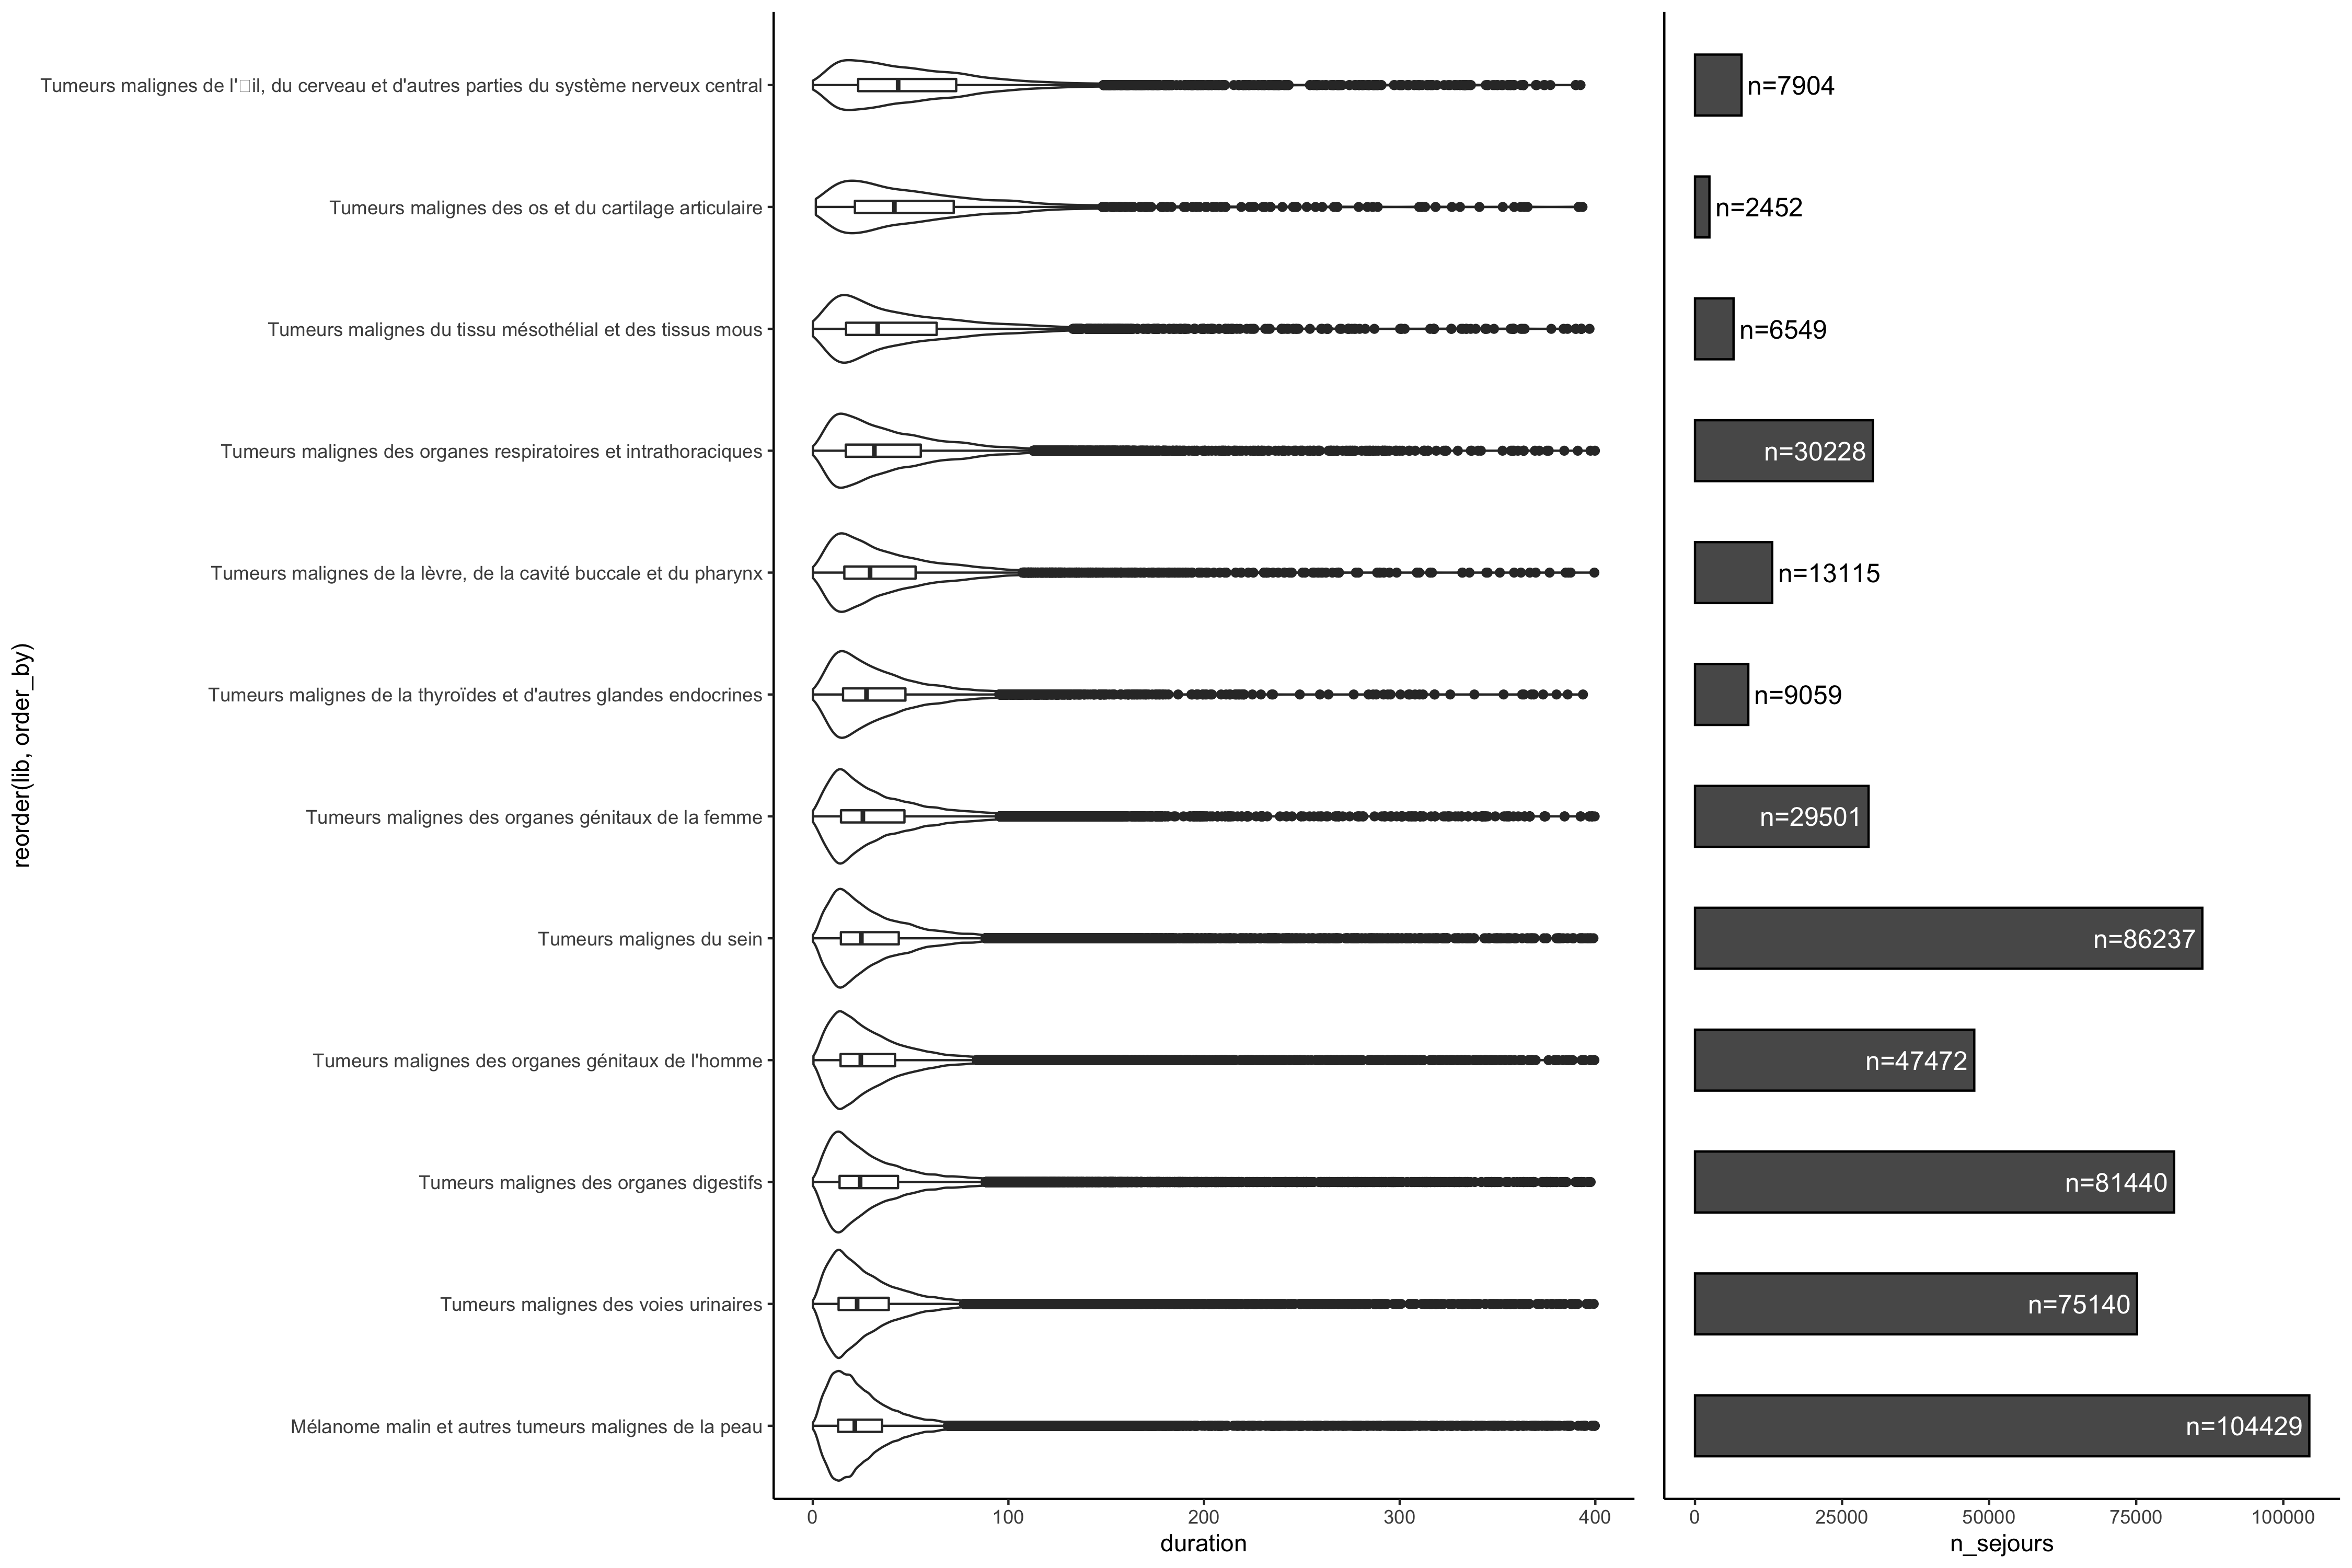
\includegraphics[width=0.9\textwidth]{images/routes/fig8_top.png}
    \centering
    \caption{ \textbf{Travel duration per cancer type.} Nice plot. }
    \label{fig:travel-duration-cancer-type}
\end{figure}

We also looked at the travel duration based on the
visited hospital. To assess the oncology specialization of the hospitals, we
used the hospitals clusters defined in (63). Only the hospitals from clusters 1
to 4 can perform cancer surgeries. Hospitals from clusters 1 and 2 are the most
specialized oncology hospitals, with all the key services such as cancer
surgery, radiotherapy, and chemotherapy. They also have the largest surgeries
volumes and are often specialized in even the rarest cancer types. Such
hospitals are sparsely located, and often placed in large cities. The hospitals
from clusters 3 and 4 are less specialized and are in both large cities and
sub-urban areas. The patients' travels were longer when they visit more
specialized hospitals from clusters 1 and 2. This might be explained by either
the need for more specialized care, or by the reputation of the hospital and the
incentive of going there in-stead of a smaller but closer hospital. We are now
interested in the spatial distribution of the patients travel duration, in
metropolitan France. On \cref{fig:routes-duration-france}, we showed the average
driving duration per municipalities on a map (A). Municipalities are filled by
duration bins. Unsurprisingly, median travel duration is short-ed for patients
living in dense municipalities. The median duration for patients living in
municipalities with more than 200 inhabitants per km\textsuperscript{2} is 16.4
minutes. However, for patients living in municipalities with less than 30
inhabitants per km\textsuperscript{2}, the median duration is 50.7 minutes,
about three times higher. Most patients living in dense areas can reach
hospitals from the more specialized clusters in little time. However, travel
durations are highest for patients from rural areas reaching the most
specialized hospitals (C).

\begin{figure}[h]
    \includegraphics[width=0.9\textwidth]{images/routes/fig1.png}
    \centering
    \caption{ \textbf{Average driving duration for cancer patients in
            metropolitan France.} Map (A) displays the average driving duration by
        municipalities. The median travel duration is higher for municipalities
        with lower population densities (B). The median travel duration is
        especially high for patients from rural areas visiting specialized
        hospitals (C). Patients living in dense areas do not need to travel far
        when reaching specialized hospitals (C). }
    \label{fig:routes-duration-france}
\end{figure}

\subsection{Travel burden index}

While travel duration is a good proxy for the patients travel burden, it is not
the only contributor. In this section, we show the results of our travel burden
score.

\begin{figure}[h]
    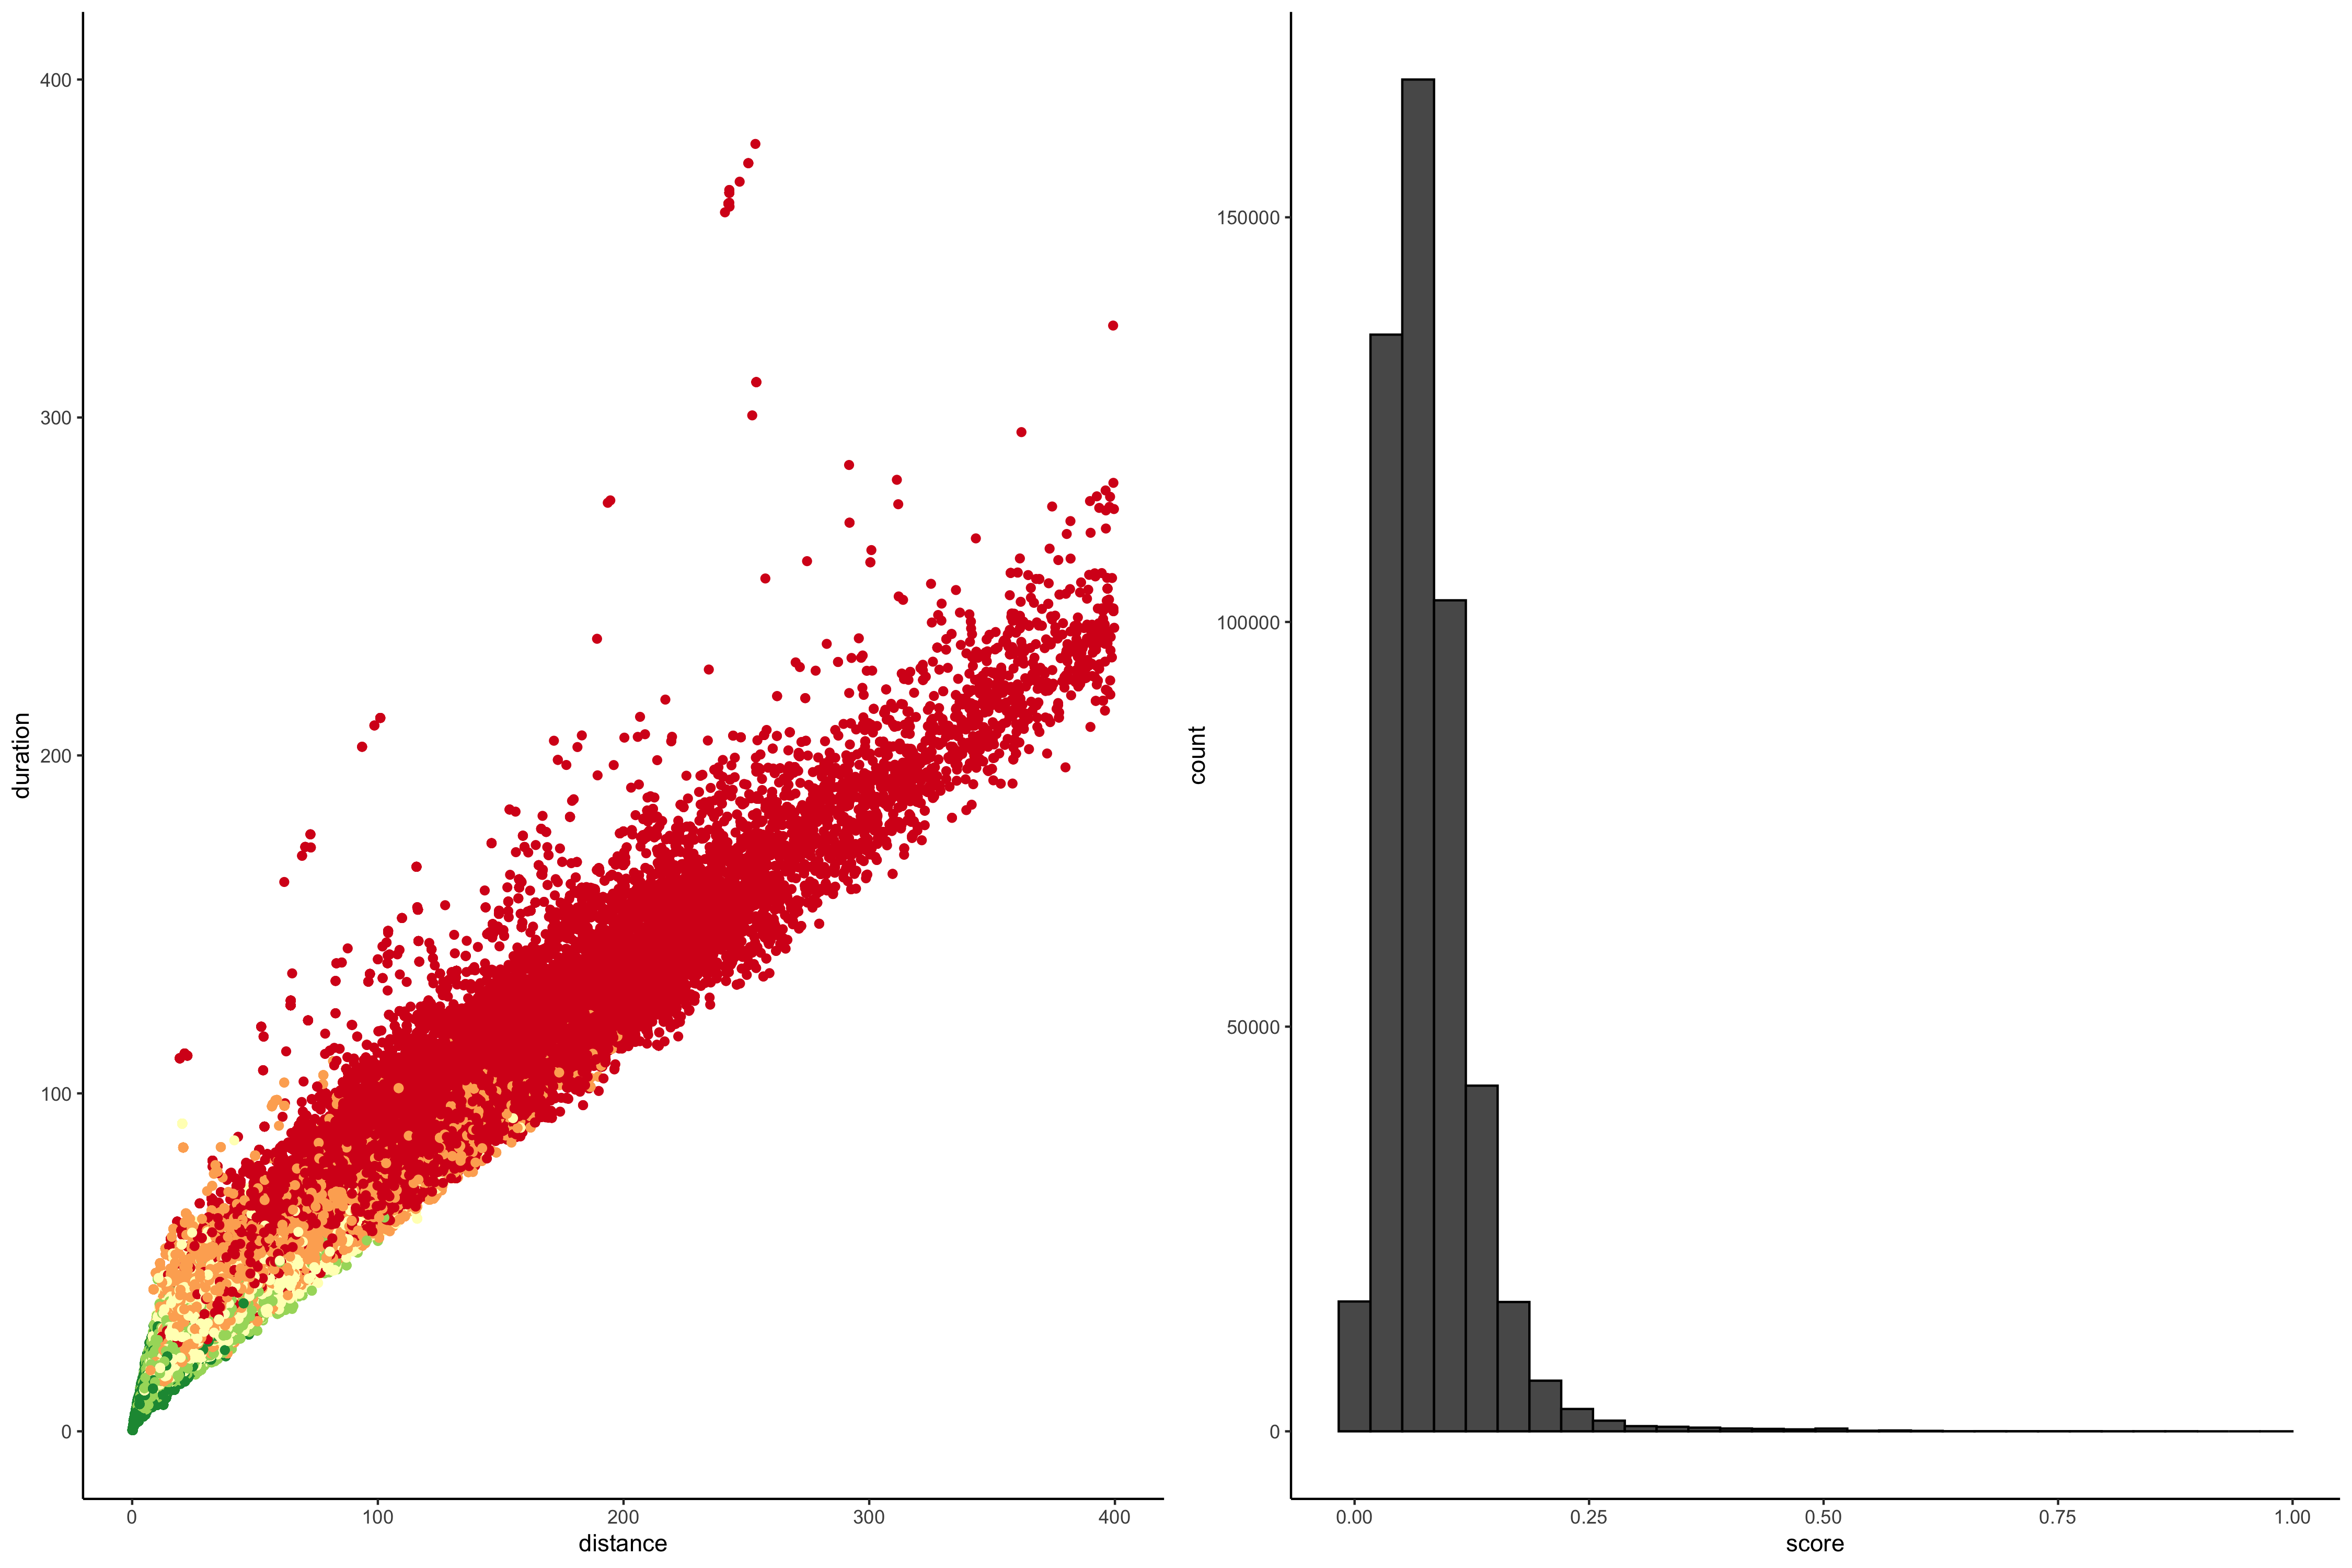
\includegraphics[width=0.9\textwidth]{images/routes/fig8_bottom.png}
    \centering
    \caption{ \textbf{Travel burden score histogram.} Nice plot. }
    \label{fig:travel-burden-histogram}
\end{figure}

On \cref{fig:routes-burden-index}, map (A) shows the spatial
distribution of the travel burden score. We display the average travel burden
score per municipality. The lower the score, the lower the travel burden is. We
discretized the average score into 5 quantiles. For municipalities in the first
quantile, the average travel burden score is in the top 20\%, meaning that
patients travel are shorts and road sinuosity is low. The first quantile is
colored in dark green on the map. The last quantile is where travel burden score
is the highest, and these municipalities are colored in pale yellow.
Municipalities with lower population densities have a higher proportion of
routes with high travel burden. For instance, among all the municipalities with
population densities lower than 30 inhabitants per km\textsuperscript{2} 47.5\%
are in the worst quantile, compared to only 19.8\% for municipalities with 200
or more inhabitants per km\textsuperscript{2} (B). We now compare the travel
burden score with several variables, such as duration, distance, sinuosity,
number of roundabouts, as well as the road type ratio (C). Higher travel burden
is associated with higher road sinuosity, distance, duration, as well as higher
number of roundabouts. The percentage of highway roads is also the highest in
this quantile.

\begin{figure}[h]
    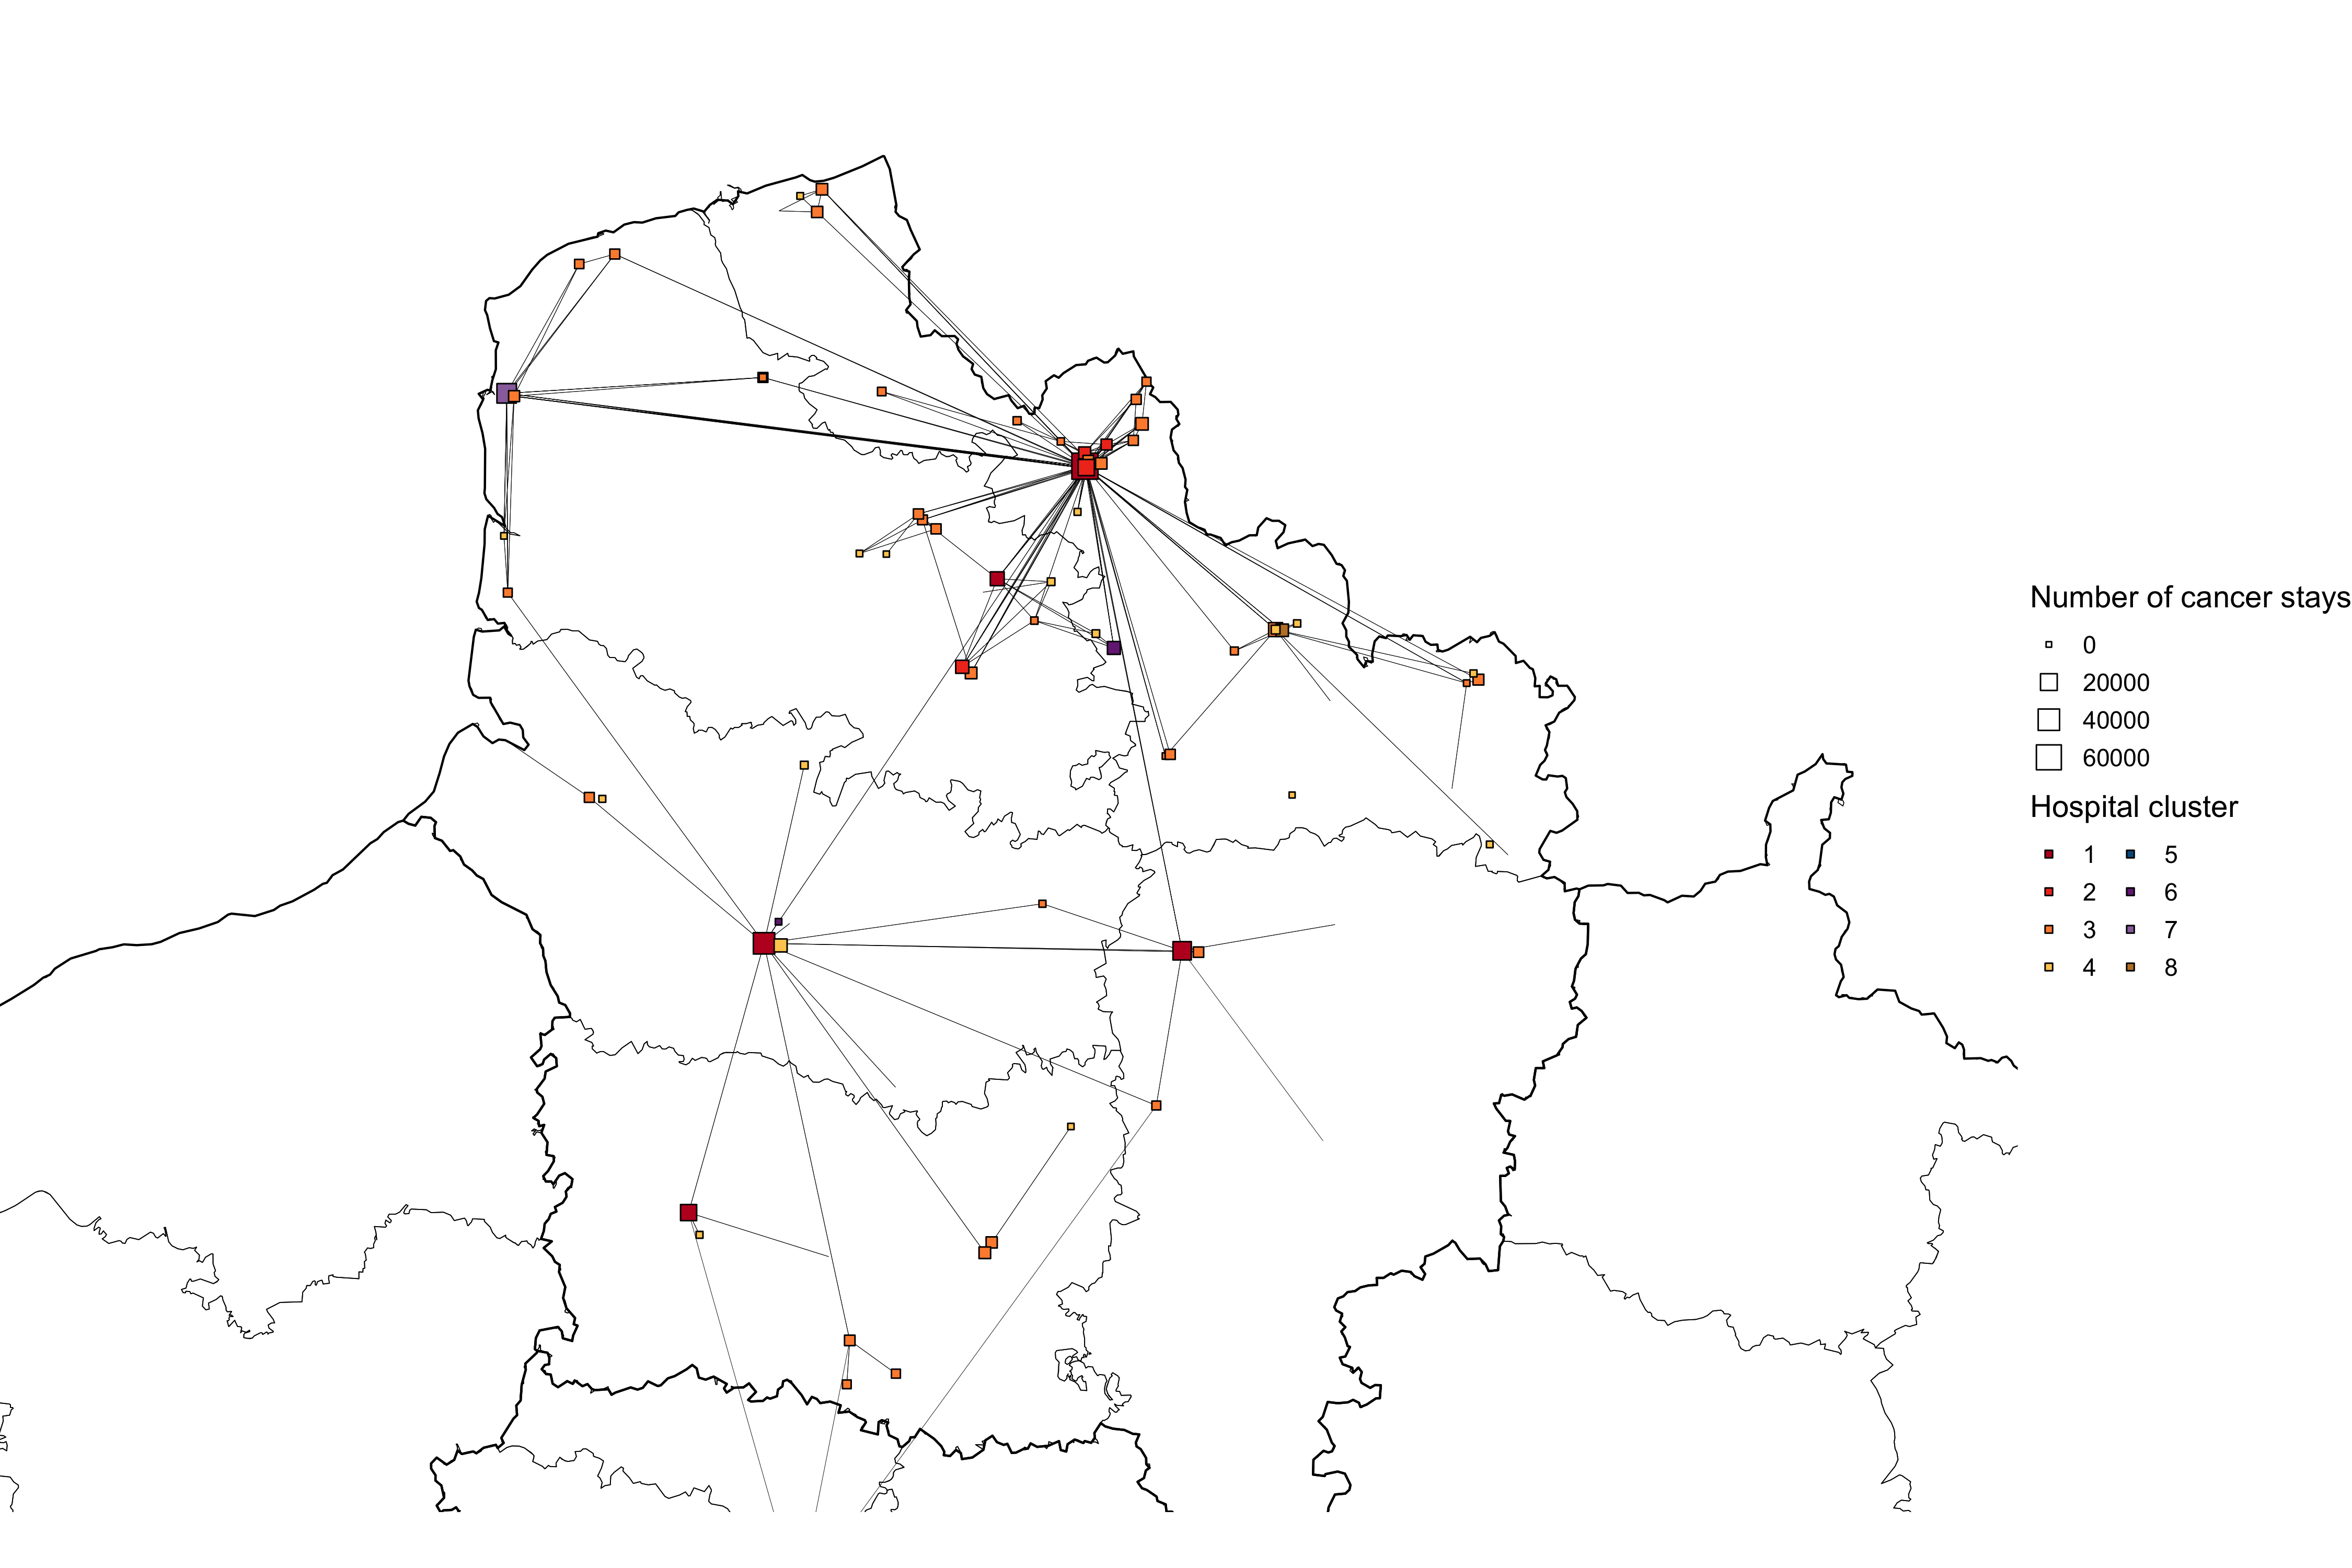
\includegraphics[width=0.9\textwidth]{images/routes/fig2.png}
    \centering
    \caption{
        \textbf{Travel burden index in metropolitan France.}
        The travel burden index is a composite score based on route duration,
        distance, number of roundabouts and sinuosity. The higher the score is,
        the more tedious the route is. The score distribution is displayed on
        map (A). The percentage of routes with higher scores increases in lower
        density areas (B). Figure (C) displays the input variables median values
        by score quantiles. For instance, the median road sinuosity is much
        higher when the score is high. }
    \label{fig:routes-burden-index}
\end{figure}

Now focusing on a single region.

\begin{figure}[h]
    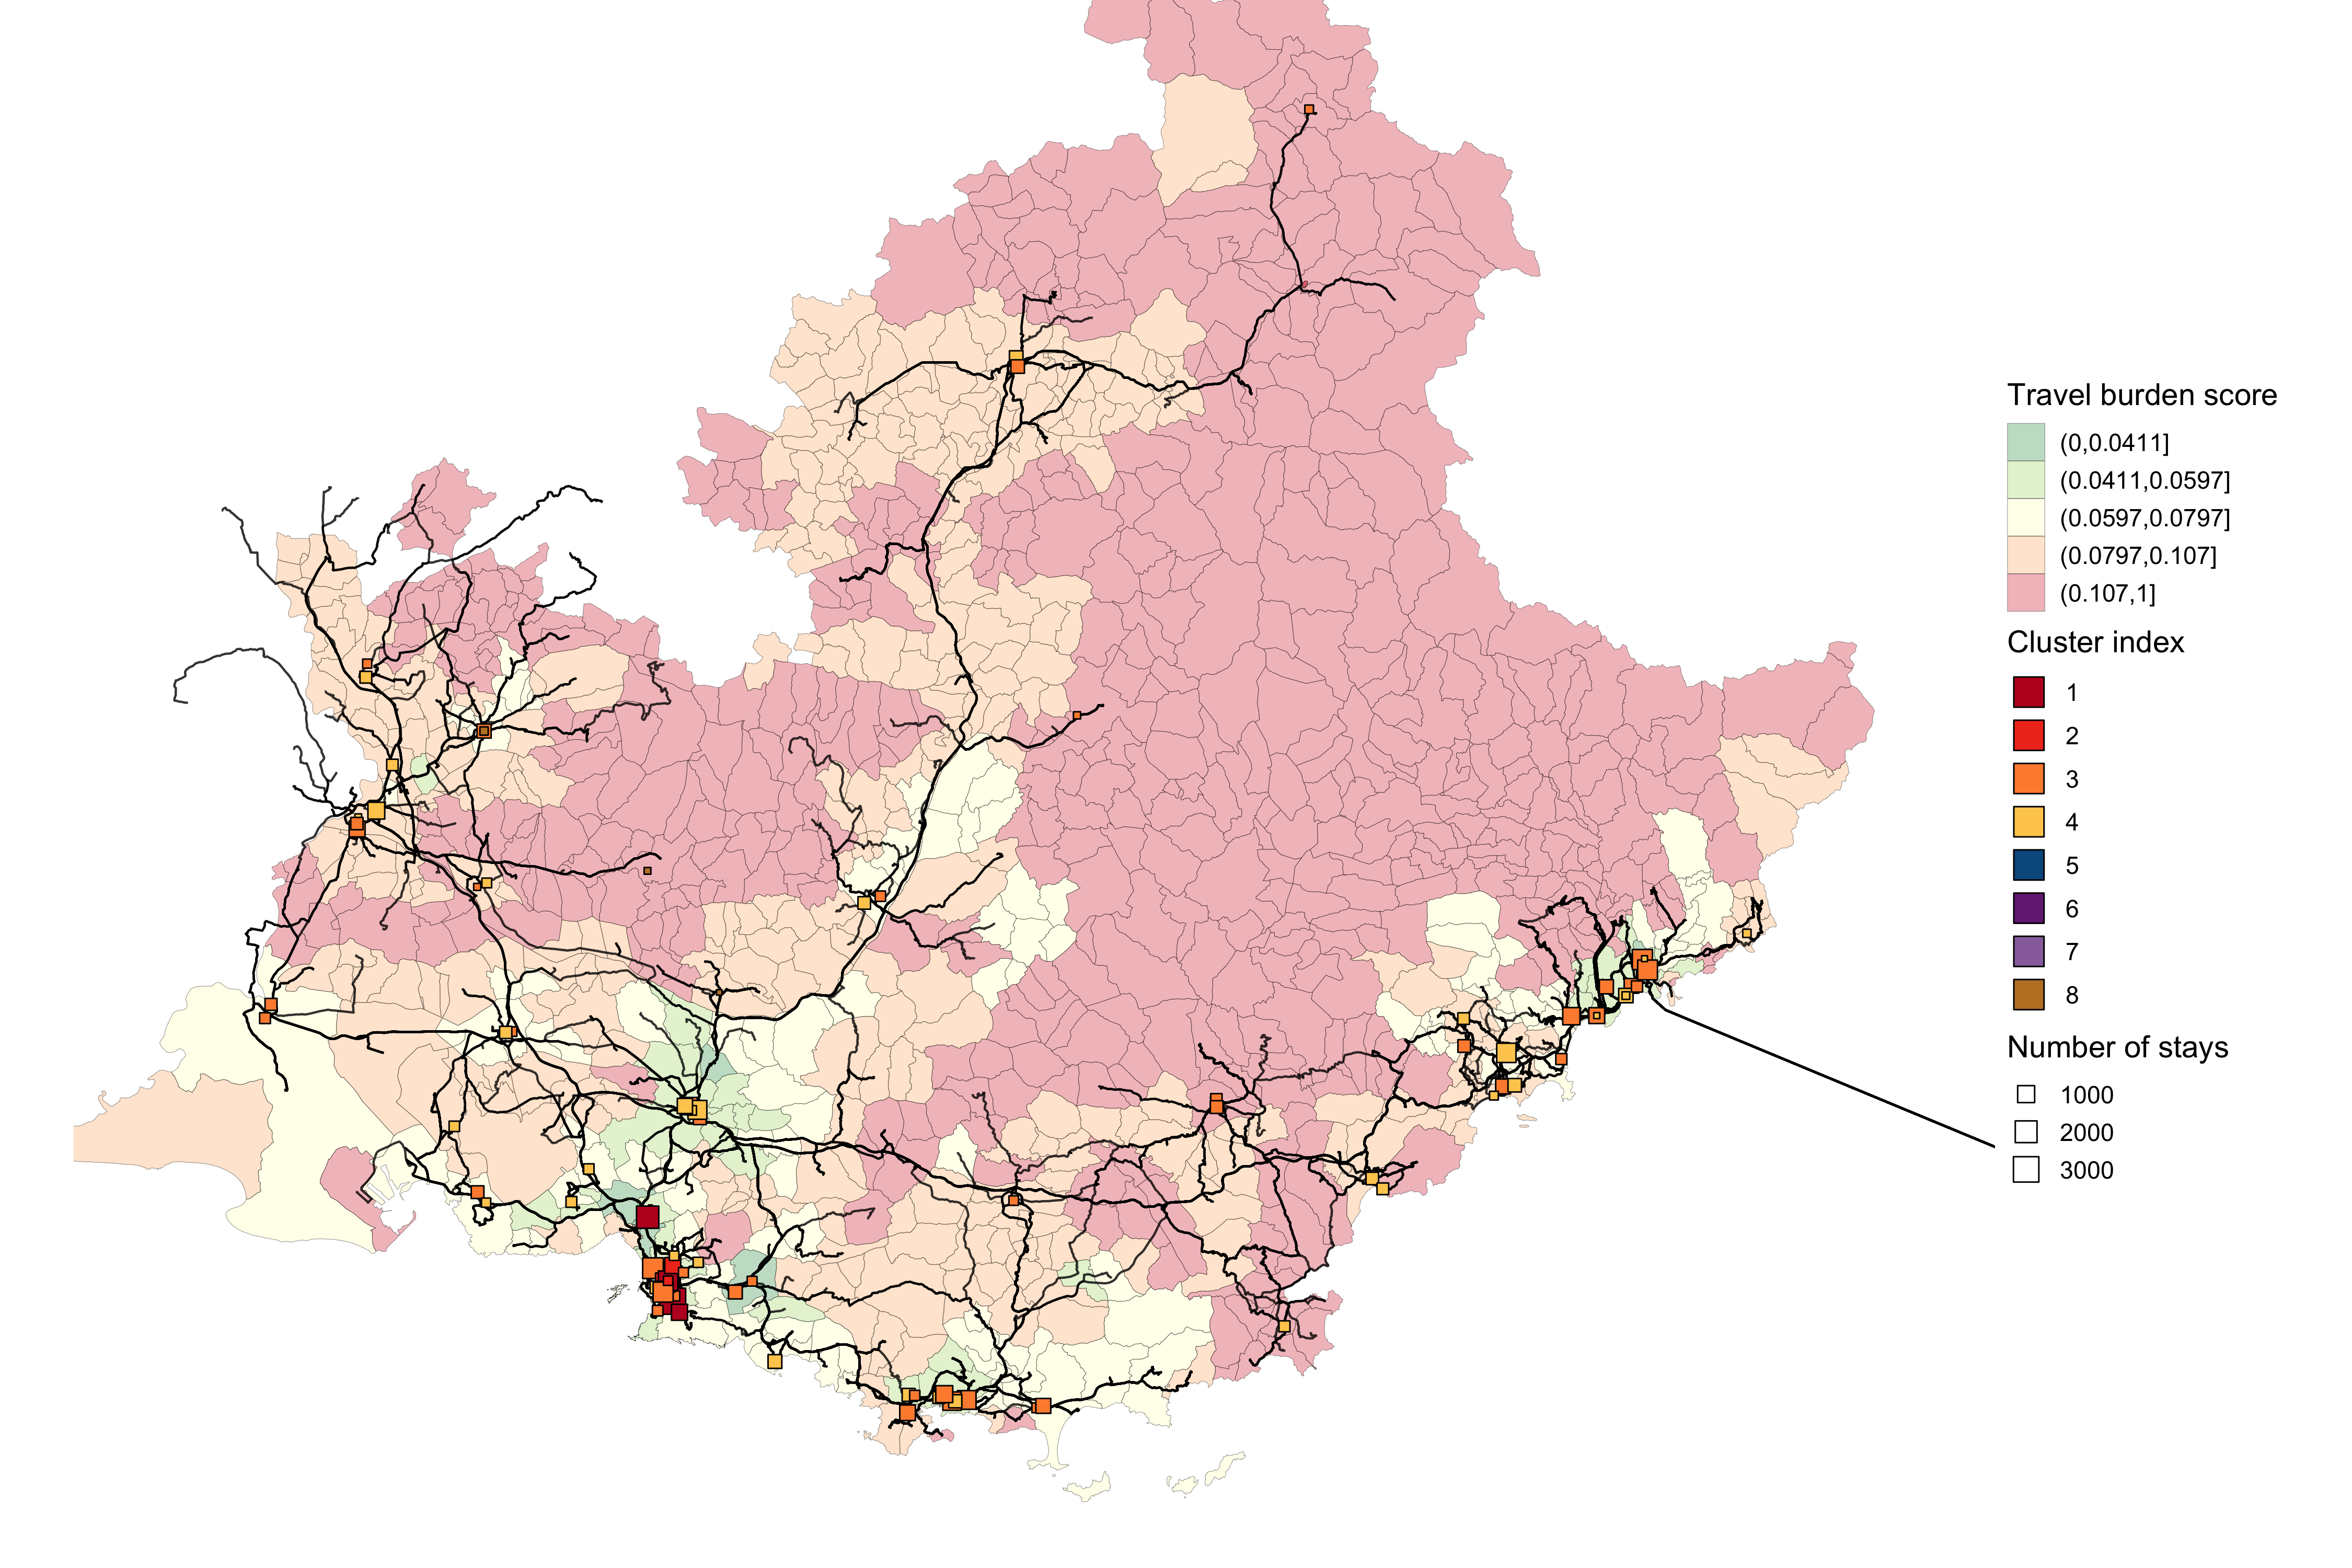
\includegraphics[width=0.9\textwidth]{images/routes/fig_7.png}
    \centering
    \caption{ \textbf{Travel burden score in PACA region.} Nice plot. }
    \label{fig:travel-duration-cancer-type}
\end{figure}

\subsection{Carbon footprint of patients travel}

We finally look at the carbon footprint of patients' travels on
\cref{fig:routes-co2-emissions}. Since we only considered direct emissions, the
carbon footprint is proportional to the traveled distance. The alluvium chart on
sub-figure (A) displays the number of patients routes between municipalities on
the left and hospitals on the right, in the Ain department, located in
Auvergne-Rhone-Alpes region. This department mostly hosts rural municipalities.
The alluvium flows are sized by number of stays and colored by the stays carbon
footprint. The darker flows indicate higher \ac{co2} emissions. We point that
the routes with the more emissions are not necessarily the routes with the most
patients. To illustrate this, we focus on the Bourg-en-Bresse city, which is the
largest city from the Ain department. On plot (B) we show the total \ac{co2}
emissions per visited hospital, for patients living in Bourg-en-Bresse.
Centre-Hospitalier de Fleyriat is the most visit-ed hospitals among patients
living in Bourg-en-Bresse, with 150 stays and 4-kilometer distance between the
municipality centroid and the hospital. The resulting \ac{co2} emissions are 72
kg. However, some patients are traveling outside of Bourg-en-Bresse to reach
hospitals based in Lyon, which represents at least an 80 km drive. For instance,
there were 18 stays in Hospital Lyon Sud, located at 91 km from Bourg-en-Bresse.
The resulting \ac{co2} emissions were 184 kg, which is more than twice the
emissions of the 150 stays in CH Fleyriat.

\begin{figure}[H]
    \includegraphics[width=0.9\textwidth]{images/routes/fig3.png}
    \centering
    \caption{ \textbf{\ac{co2} emissions for cancer patients travels} The
        \ac{co2} emissions are computed based on the GPS distance between the
        patient municipality centroid and hospital location. The total emission
        for a single travel is computed as the product of the average \ac{co2}
        emissions per km and the distance. Figure (A) displays the travels
        between municipalities in Ain department. Municipalities are on the
        left, hospitals on the right. Flows are sized by number of travels and
        colored by \ac{co2} emissions. Figure (B) shows the \ac{co2} emissions
        compared with number of stays in Bourg-en-Bresse city (Ain). The
        \ac{co2} emissions are higher for the fewer patients who traveled
        outside of the city to reach more specialized care centers in Lyon. }
    \label{fig:routes-co2-emissions}
\end{figure}

\section{Discussion}

The results of the travel analysis for cancer patients in metropolitan France
concur with the effects of regionalization of care observed in the literature.
We report longer travels for patients living in rural areas. The hospitals
specialized in oncology tend to receive patients from more distant population
locations. Finally, patients with less frequent cancers are forced to travel
further due to the limited number of hospitals that can correctly treat these
pathologies. We introduced the travel burden score, a new metric to consider
when studying patients travels. This score is proportional to not only distance
and duration, but also road sinuosity and number of roundabouts. The last two
variables, which are not explicitly captured by distance and duration, could be
responsible of more tedious drives for the patients, especially when their
health conditions are deprived. In our estimation, the \ac{co2} emissions are
directly proportional to the traveled distance. We did not consider indirect
emissions linked to the transportation. Car was the only transportation mean we
used, and we assumed every patient traveled by car, which might over-estimate
the \ac{co2} emissions. More research is needed to include public transportation
such as train or subway. The larger share of carbon emissions for cancer
surgeries is covered by frequent cancers, that can be treated in many hospitals,
like breast cancer for instance. For such pathologies, a rethink of the
regionalization of care model might be needed. Patients from less dense
municipalities could be sent to closer regional hospitals if we make sure the
surgeons' expertise is good enough. Partnerships with larger and more
specialized hospitals could be created to spread the more up to date knowledge
outside the urban hospitals. However, this will be more complicated for rare
cancers, where expertise is scarce and concentrated in the larger hospitals. On
a carbon footprint perspective, we believe the lower number of concerned
patients makes it less of a priority.

  \chapter{Transparency in healthcare}

\section{Context}

\subsection{The communications revolution}

Over the past few years, there has been a massive change in the way we
communicate and interact with information. The amount of data and content
available to the public keeps increasing, as well as the number of information
delivery platforms. Studies define this phenomenon as ``the communications
revolution'' \cite{viswanath_communications_2012}. Smartphones democratization
and adoption rate are partly responsible for this revolution. Indeed, a large
and growing number of people own a smartphone, enabling them to access
information anytime and anywhere. Through this, there has been a change in how
people access and use information. With the increasing number of media sources,
mass audience is now split into smaller groups who share common characteristics
and interests. Also, the growth of online audience is now far outpacing the
other media. As a benefit of this communication revolution, it is getting easier
to access resources online, even technical resources such as technical reports
and scientific articles. While these materials may not always be intended for a
mainstream audience, their availability offers opportunities for access and
interpretation by different groups.

\subsection{Healthcare online resources}

The healthcare sector is no exception in this revolution, and health resources
are increasingly available online
\cite{viswanath_science_2005,viswanath_communications_2012}, changing how
patients interact with health providers. Communication has been found to play a
central role in cancer prevention and control. It can provide information on
cancer prevention, monitor lifestyles and health behaviors, promote
participatory decision making during cancer detection, diagnosis, and treatment,
and foster quality of life during survivorship or end of life
\cite{viswanath_communications_2012}. When diagnosed with cancer patients and
their family members lives change radically. They receive treatments and have to
make choices with serious consequences. Such diseases and treatments are
complex, but should be understood before decisions are made. Patients and their
family members should be provided with intelligible and up to date information
on the stage of disease, treatment options and complementary therapies
\cite{butow_dynamics_1997,cassileth_information_1980}.

Multiple benefits of bringing more information to the patients have been
reported. Involving cancer patients in decision-making on their pathways
improves their satisfaction and quality of life, compliance with treatment and
their ability to manage symptoms
\cite{johnson_effects_1982,hack_feasibility_1999,mohide_randomised_1996,mcpherson_effective_2001,
    sheabudgell_information_2014,huchcroft_testing_1984,cegala_patient_2003,viswanath_science_2005}.
Moreover, medically related education interventions are most effective when they
are tailored to patients' individual needs, especially for cancer patients
\cite{cegala_patient_2003}. Through all these benefits, it is clear that
monitoring patient information seeking experiences over time is important
\cite{finney_rutten_cancer-related_2016}.

\subsection{Patients information seeking}

As a matter of fact, patients are often seeking information during their
pathways. In the United States of America, a survey from the Health Information
National Trends (HINTS) \cite{hesse_trust_2005} measured online health
activities, levels of trust, and source preference for 6,369 people. They
observed that physicians remained the most trusted source of information,
despite an increasing number of people looking for information online.

However, there is increasing evidence in the literature that patients are often
not satisfied with the information they received. Some reported to lack
information on their disease and its consequences
\cite{mcpherson_effective_2001}, while others forget or misunderstand the
information conveyed \cite{ley_communicating_1988,hogbin_getting_1989}. The
interaction with their physician has also been cited as a major cause of
dissatisfaction \cite{stewart_effective_1995,bartlett_effects_1984} at all
stages of illness \cite{higginson_palliative_1990}. Patients reported
insufficient time spent on communication during the clinical encounter and
physicians inability to keep up with the most current information and advances
in cancer care \cite{anderson_impact_2003}. Some patients reported incorrect
diagnosis, or not receiving the most up-to-date cancer information from their
physician, especially for rare cancers \cite{dolce_internet_2011}. Patients who
need health information but experience difficulties have been found at risk of
experiencing poorer psychosocial health \cite{arora_barriers_2002}.

A Canadian study surveyed patients attending appointments at follow-up cancer
clinics in Calgary, Alberta \cite{sheabudgell_information_2014} between 2011 and
2012. They approached 648 patients and obtained responses from 411 one of them.
The study aimed at: identifying information needs of patients when meeting their
physician for a follow-up; listing patients preferences on how to receive
information. Here are the results they gathered regarding information seeking
patterns. The most frequently reported source of information was the Internet
(57.4\%); health provider (32.6\%), brochures or pamphlets (25.1\%), and cancer
organizations (24.3\%). The most frequently reported types of information sought
included information about a specific type of cancer (43.1\%), treatment or
cures for cancer (29.4\%), prognosis or recovery from cancer (29.0\%), and
prevention of cancer (27.0\%). The least frequently reported types of cancer
information sought included where to get medical care (3.4\%), paying for
medical care or insurance (4.6\%), and cancer organizations (5.4\%). Regarding
trust, the physician or health care provider was largely the most trusted source
of information, followed by Internet, and family and friends. The least trusted
sources of information included radio, newspaper, and television.

More evidence is reported on the use of the internet for health information
retrieval
\cite{chen_impact_2001,pereira_internet_2000,ziebland_how_2004,dolce_internet_2011}.
For instance, an online questionnaire was administered to participants of
cancer-related communities hosted by the Association of Cancer Online Resources
(ACOR) \cite{dolce_internet_2011}. As a result, 488 participants shared their
personal experiences on why and how they accessed online health resources.
Participants who experienced a lack of informational support related to
procedures found blogs and testimonies online that helped them to know what to
expect from a physical and emotional perspective. Moreover, for rare diseases,
physicians might actually benefit from patients looking from additional
information online, as it could bring additional knowledge to them, and even
change their plans for care. Aware patients can also challenge their physicians
by asking meaningful questions and participate in the tailoring of their
treatment plans. Finally, online communities allowed patients to identify
physicians with a proven track record in cancer care. They endorsed care
providers who took the time to answer questions, as well as specialists from
major cancer centers, that brought superior care which led to better outcome.
Indeed, \ac{gp} play a crucial role in early cancer detection because the
majority of cancer patients initially consult their \ac{gp} with symptoms.
Therefore, the actions taken by the \ac{gp} upon the patient's symptom
presentation may considerably affect the cancer trajectory
\cite{flytkjaer_virgilsen_cancer_2019}. To sum up, the increased usage of the
Internet by cancer patients puts new demands on health care professionals.
Patients need advice about how to find reliable and credible web sites and also
help with authenticating and interpreting the information they find
\cite{carlsson_cancer_2009}.

\subsection{Bringing transparency in cancer surgery}

While patients are looking for informations on their symptoms, diseases and
treatments, it would be crucial for them to know better about their physician's
ability, especially for cancer surgery. In cancer care, surgery is one of the
most important part of the treatment, and is directly linked to the surgeon
ability.

Surgeon and hospital-related factors have been found to be direct predictors of
outcome in colorectal cancer surgery \cite{renzulli_influence_2006,
    bonati_surgeon_2021}. In breast cancer, patients managed by high-volume surgeons
were more likely to have breast-conserving surgery (BCS) than those managed by
low-volume surgeons \cite{mcdermott_surgeon_2013}. Moreover, breast cancer
patients who receive treatment from experienced and specialized surgeons are
more likely to receive the standard sentinel lymph node biopsy
\cite{yen_surgeon_2014}. The surgeon's expertise and learning curve is directly
related to the patient's outcome \cite{renzulli_learning_2005}. A low surgeon or
hospital caseload may be compensated by intensified supervision or by improved
training and teaching \cite{bonati_surgeon_2021}. From all these findings, it is
questioned whether surgeons should have an ethical obligation to inform patients
of their surgical volume and outcomes \cite{glaser_surgeon_2019}. One way to
monitor the surgeons abilities is the use of quality indicators, which have been
developed in high income countries and contributed to improved quality of care
and patient outcomes over time \cite{nietz_quality_2020}.

\section{Methods}

With these evidences of healthcare information needs, we developed Healthcare
Network, a web application that lists every hospital in France, and displays key
statistics on them. The application is directed to either health professionals
or patients. Health professionals might use it to gain insights about specific
hospitals, and look for the best place to send their patients when they lack
expertise. Patients could learn more about the hospital they have been sent to,
check the care quality or surgery volume.

To create the Healthcare-Network web application, we centralized the several
datasets into databases. We then built the backend of the application with
Python and Flask framework, while the frontend was coded with HTML and CSS from
the Bootstrap library. We used two databases: a relational database (MySQL) and
a no relational database (Mongo DB). In Mongo DB, we stored the datasets to draw
the interactive maps in the application. We used the geojson format, which works
well with Mongo DB. All the other datasets are stored in the relational
database. There are roughly 40 tables in the relational database. The most used
tables are statistics on the hospitals and on the municipalities. We chose to
use the Flask framework for its simplicity and the high number of users. The
framework has a simple core to quickly build a working web application with
little code. It can be improved with extensions that add new features. With such
framework, we built several API routes that render HTML and CSS templates to the
users. The interactive maps were built with the Folium library, and the other
figures with Plotly.

\section{Results}

In this section, we will describe the most important features of the web
application, illustrated with screen captures from the website.

The landing page of the application is a minimalist search bar, as illustrated
on \cref{fig:hn-home}. The search feature lets the user look for hospitals by
name, category or location. In this first version, the search algorithm is
fairly basic and matches the hospitals that contains the text query in either
its name category or location. No weighting or additional rule was added. The
search feature could be improved later on, by using dedicated and search focused
databases like the very popular Elastic Search.

\begin{figure}[h]
    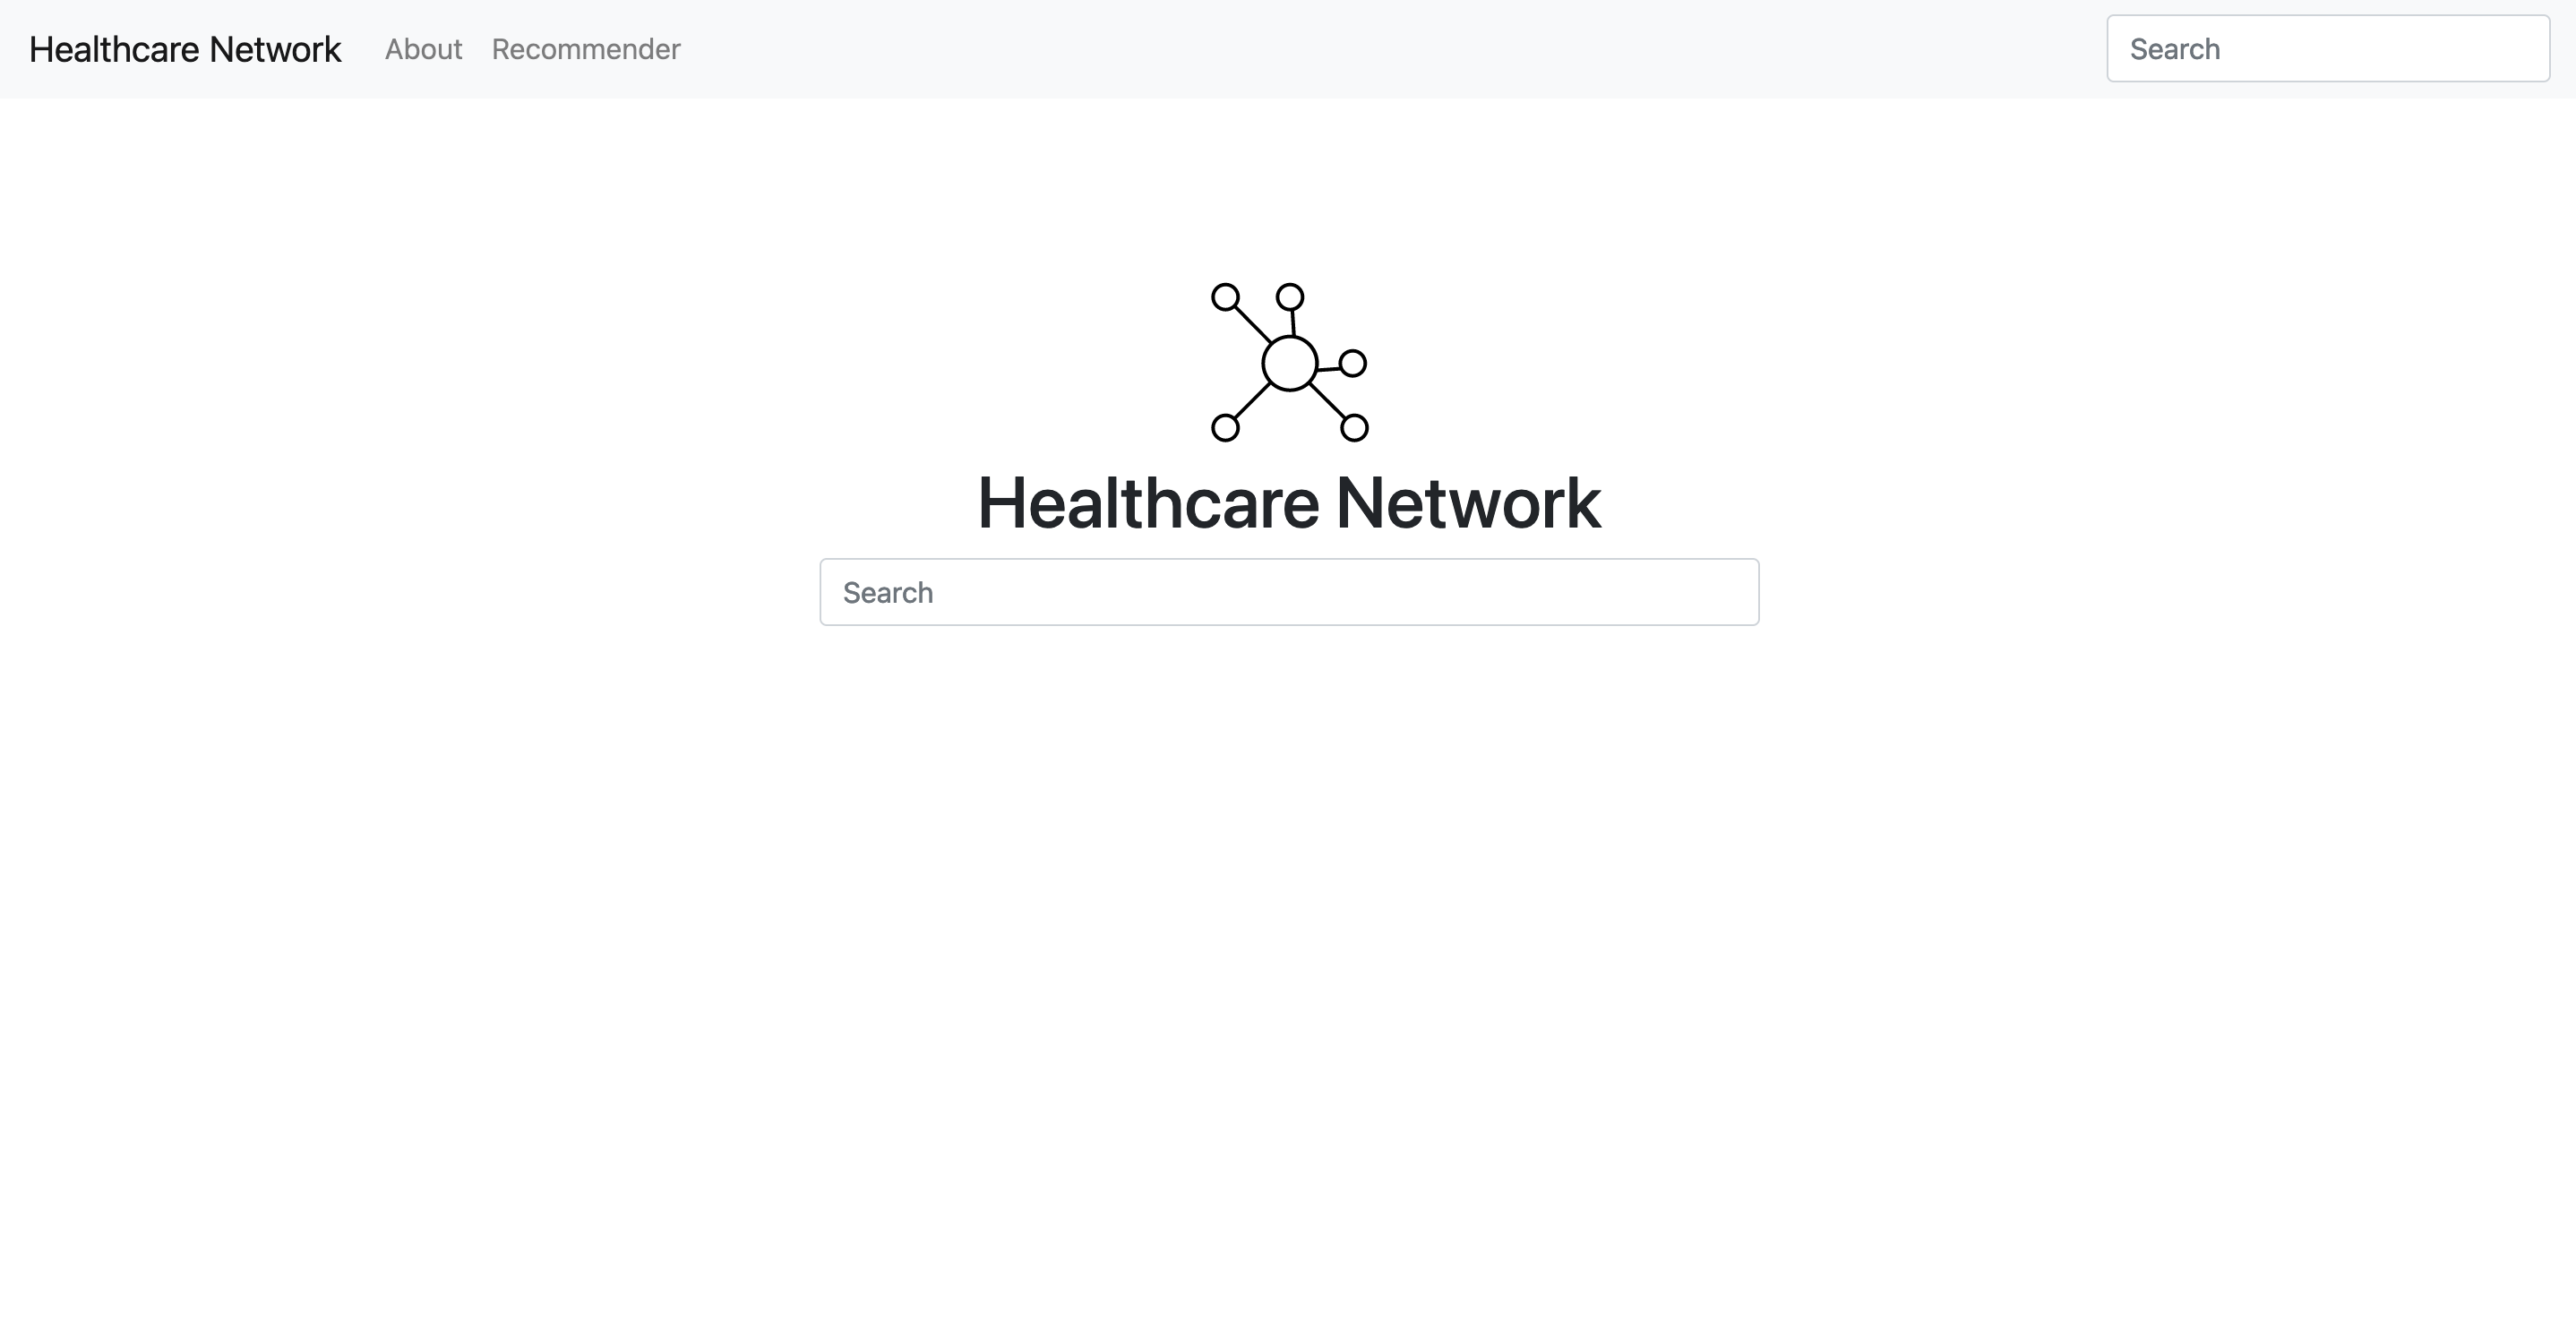
\includegraphics[width=0.7\textwidth]{images/healthcare-network/home.png}
    \centering
    \caption{ \textbf{Healthcare-Network: homepage.} A minimalist page with a
        search bar allowing to find hospitals based on their name, category, or
        location. }
    \label{fig:hn-home}
\end{figure}

We now provide a search example, and \cref{fig:hn-search} shows the results of
the query ``chu'', corresponding to the \acf{chru} hospital category. 153
results were returned, displayed as a list on the left and on a map on the right
side of the screen. The list shows basic informations about the retrieved
hospitals, including their names, locations, categories and type of care
provided, like \acf{mco} for instance. The map is interactive, and lets the user
visualize the spatial distribution of the retrieved hospitals. On the map, the
hospitals are displayed as icons, colored by hospital category. This query
illustrates an additional feature of the search bar: show the spatial distribution
of the hospitals in France by category.

\begin{figure}[h]
    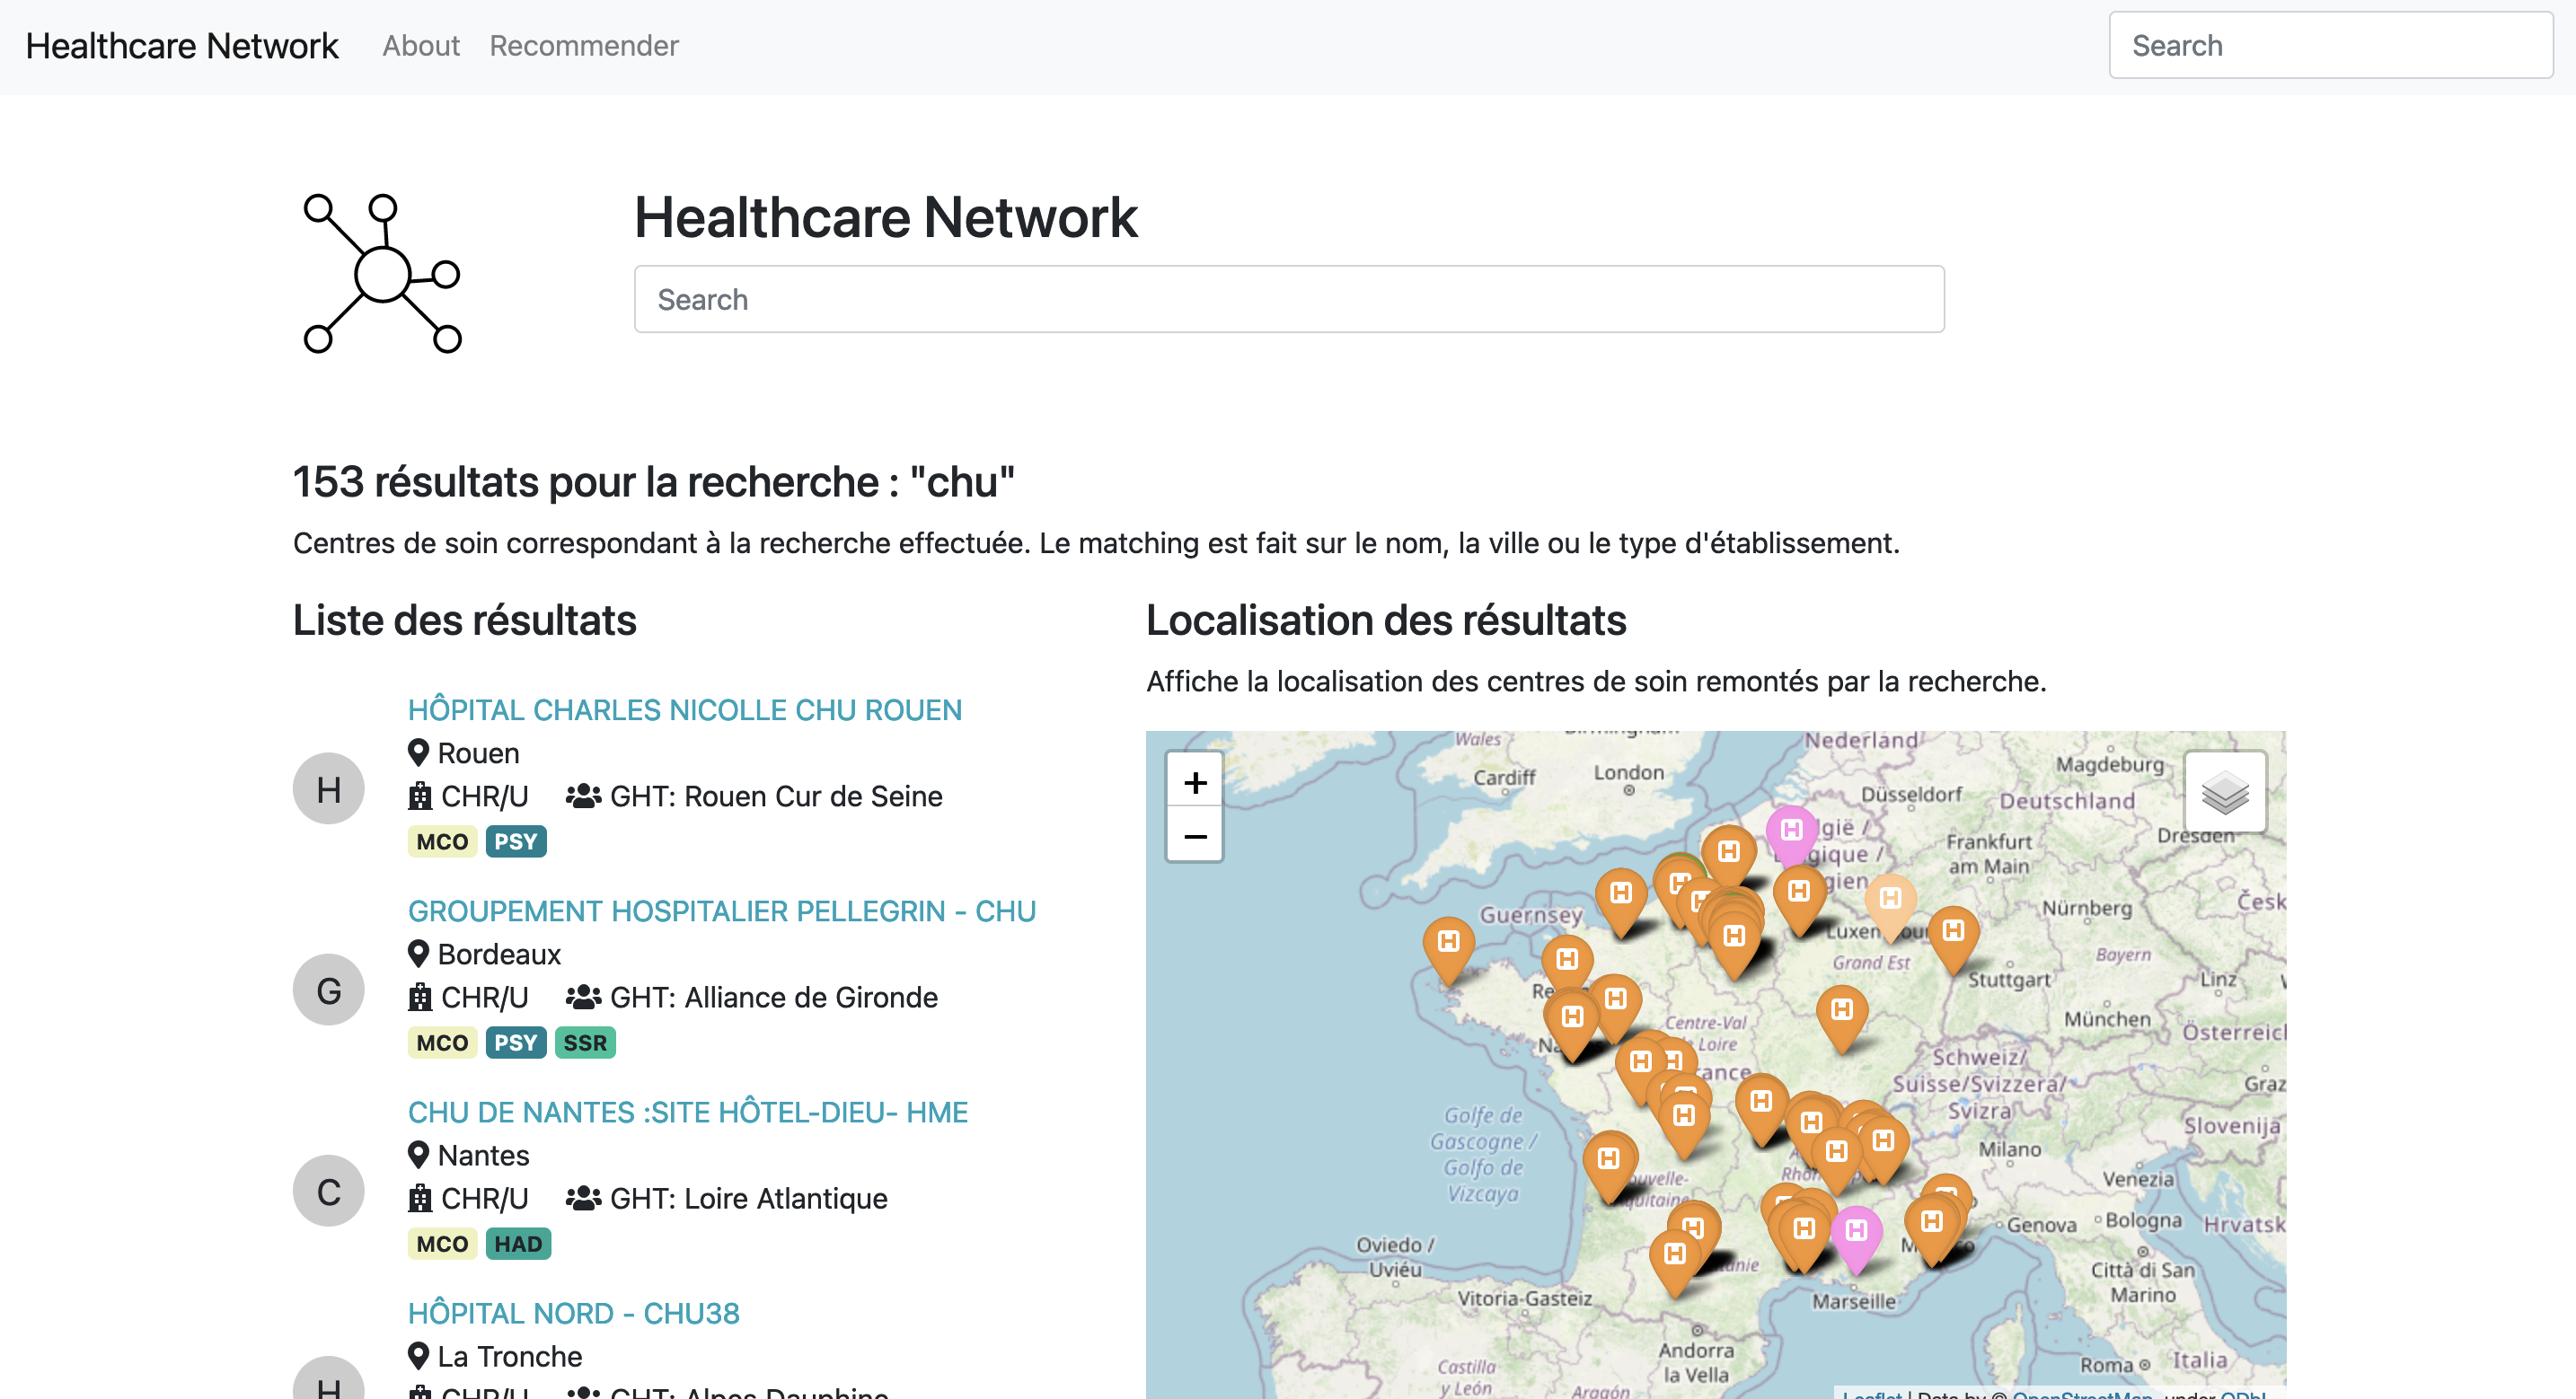
\includegraphics[width=0.7\textwidth]{images/healthcare-network/search.png}
    \centering
    \caption{ \textbf{Healthcare-Network: search results.} The list of retrieved
        hospitals and their details is displayed, as their position on a map.
        This query shows all the \ac{chru} hospitals in metropolitan France. }
    \label{fig:hn-search}
\end{figure}

Each hospital has its individual web page, as illustrated on
\cref{fig:hn-coulommiers-page} with the \ac{ch} de Coulommiers. The web page
shows basic informations about the hospital, with name, location and category
displayed first. A navigation pane also shows the hospitals from the same
\ac{ght} and legal entity. Hospitals within the same \ac{ght} share their
information system. This grouping was introduced in 2016 for the public
hospitals only. They aimed at facilitating the communication between these
facilities, and make it easier to transfer patients from one hospital to another
if needed. Hospitals from the same legal entity are governed by the same
administration, but spread among multiple geographical sites. Hospitals in large
cities such as Paris, Marseille or Lyon have most of their largest hospitals
belonging to the same legal entity. For instance in Paris, the AP-HP legal entity
gathers 39 hospitals spread across the Ile-de-France region.
The hospital location is shown on an interactive map, where the user can
zoom in and out, and add more indicators, including:

\begin{itemize}
    \item The municipalities populations and median salary. These indicators are
          a way to gain insight about the hospital neighborhood, and neighboring
          demand. To display these indicators, we color the municipality according
          to the indicator value.
    \item Patients provenance. We display the number of patients who visited
          this hospital per municipalities within a year. Through this, it is
          easy to evaluate how influent and important an hospital is, based on
          how many patients it is draining from further population locations.
          Usually, small local hospitals tend to receive patients from their
          immediate neighborhood; where large hospitals specialized in oncology
          like Institut Curie or Institut Gustave Roussy will treat patients
          from many different regions.
    \item Other hospitals from the same \ac{ght}. We display on the map the other
          hospitals that share the same information system. With this information,
          we can evaluate how close this hospital is to other hospitals where it
          would be easy to transfer patients if the desired pathology is not treated
          in this hospital.
    \item Other hospitals that shared patients with this hospital within a year.
          We call this 'co-occurrences', and a higher number shows that two
          hospitals seems to work closely together. For instance, one hospital
          might handle the cancer surgery and send their patients to another
          hospital for radiotherapy. Identifying hospitals that frequently
          exchange patients is a good way to find alternative hospitals for
          certain pathologies. There is also a high chance that these two
          hospitals communicate frequently with each other, making it easier
          to send patients and keep track of what happened in their pathways.
\end{itemize}

\begin{figure}[h]
    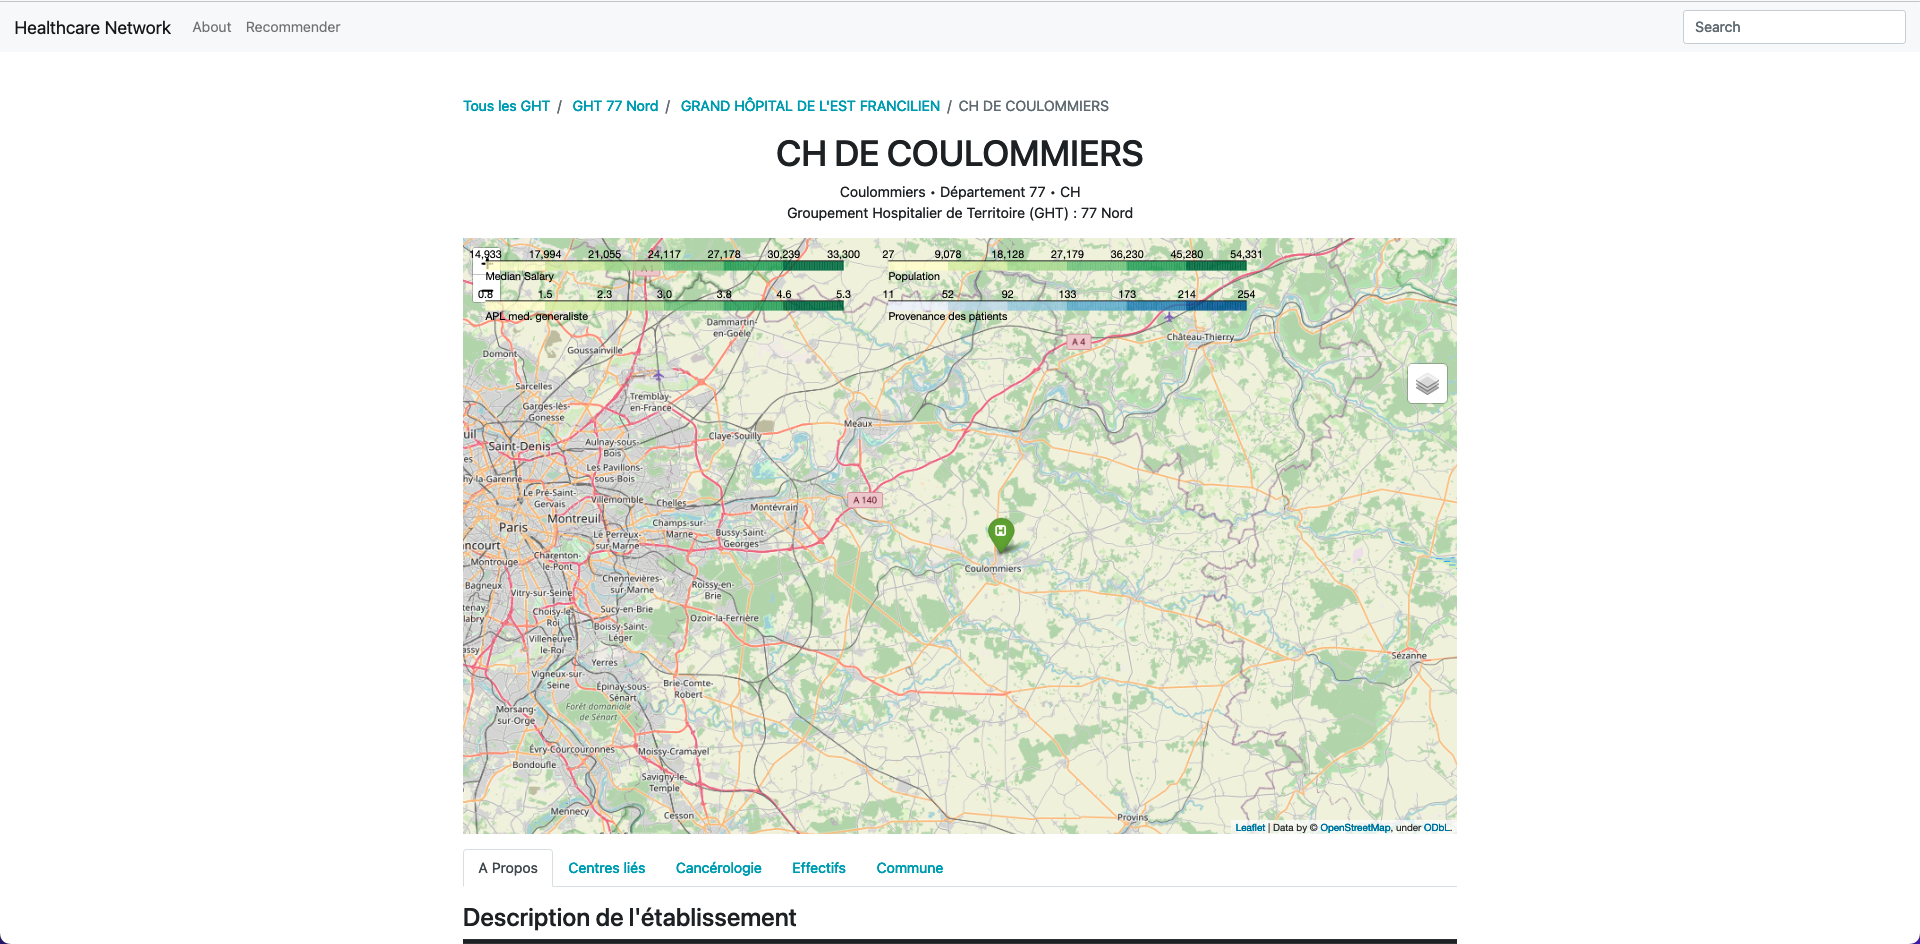
\includegraphics[width=0.7\textwidth]{images/healthcare-network/hospital-page.png}
    \centering
    \caption{ \textbf{Healthcare-Network: example of an hospital page, \acf{ch}
            de Coulommiers.} The web page shows basic informations about the
        hospital, with name, location and category displayed first. A navigation
        pane also shows the hospital \ac{ght} and legal entity. The hospital
        location is shown on an interactive map. }
    \label{fig:hn-coulommiers-page}
\end{figure}

The \cref{fig:hn-coulommiers-co-occ} is an example of the interactive map
mentioned earlier. Here, we colored the municipalities by the number of patients
who visited \ac{ch} de Coulommiers. We also displayed hospitals from the same
legal entity in green. Finally, we show hospitals that exchanged patients with
\ac{ch} de Coulommiers as blue links. From this map, we observe that \ac{ch} de
Coulommiers mostly attract patients from the neighboring municipalities. The
hospitals with the most co-occurrences are either from the same \ac{ght}, or
located in Paris. This might mean that patients with complications were sent to
larger hospitals in Paris.

\begin{figure}[h]
    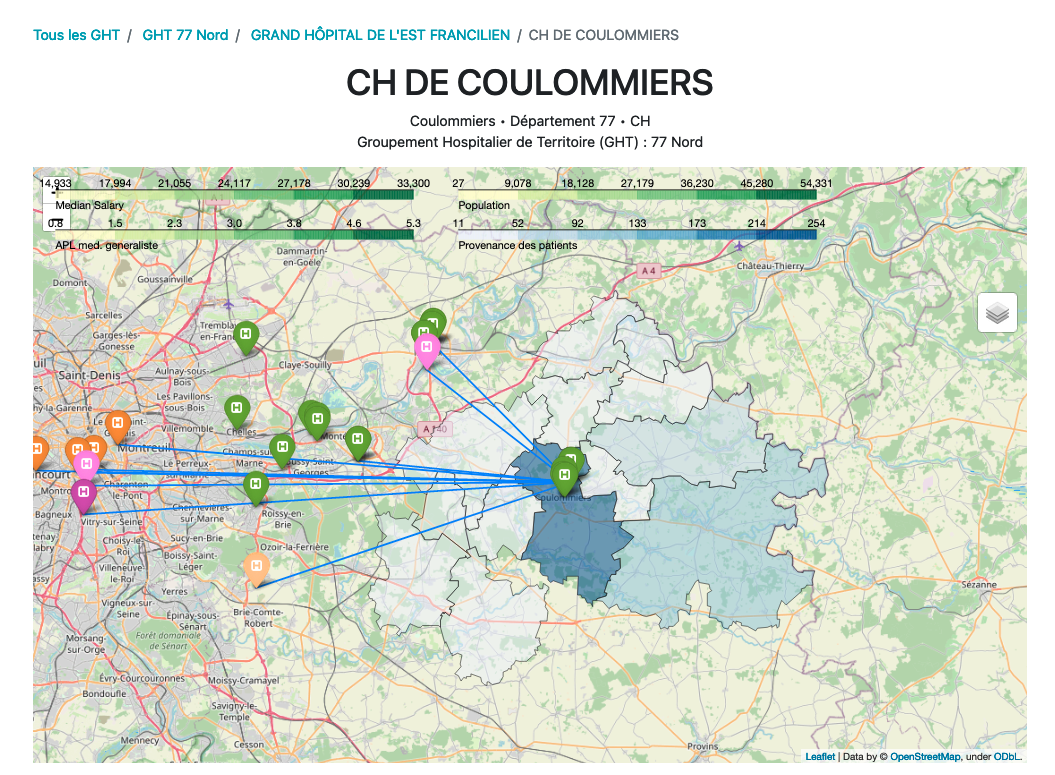
\includegraphics[width=0.7\textwidth]{images/healthcare-network/coulommiers-co-occ.png}
    \centering
    \caption{ \textbf{Healthcare-Network: example of an hospital page, \acf{ch}
            de Coulommiers.} We filled the municipalities by the number of patients
        who visited \ac{ch} de Coulommiers. We also displayed hospitals from the
        same legal entity in green. Finally, we show hospitals that exchanged
        patients with \ac{ch} de Coulommiers as blue links. }
    \label{fig:hn-coulommiers-co-occ}
\end{figure}

Below this interactive map, we display the list of services and number of
\ac{mco} stays and beds for hospitals. For instance, on
\cref{fig:hn-curie-services}, we displayed this information for the Institut
Curie Paris hospital. The list of services allows to quickly evaluate the
hospital ability to treat cancer patients. The number of stays and number of
beds lets the users evaluate the hospital size, and how saturated it is. We see
that Institut Curie has all the main services besides psychiatry and palliative
care. From the activity statistics, we see that this hospital does not do any
obstetric activity.

\begin{figure}[h]
    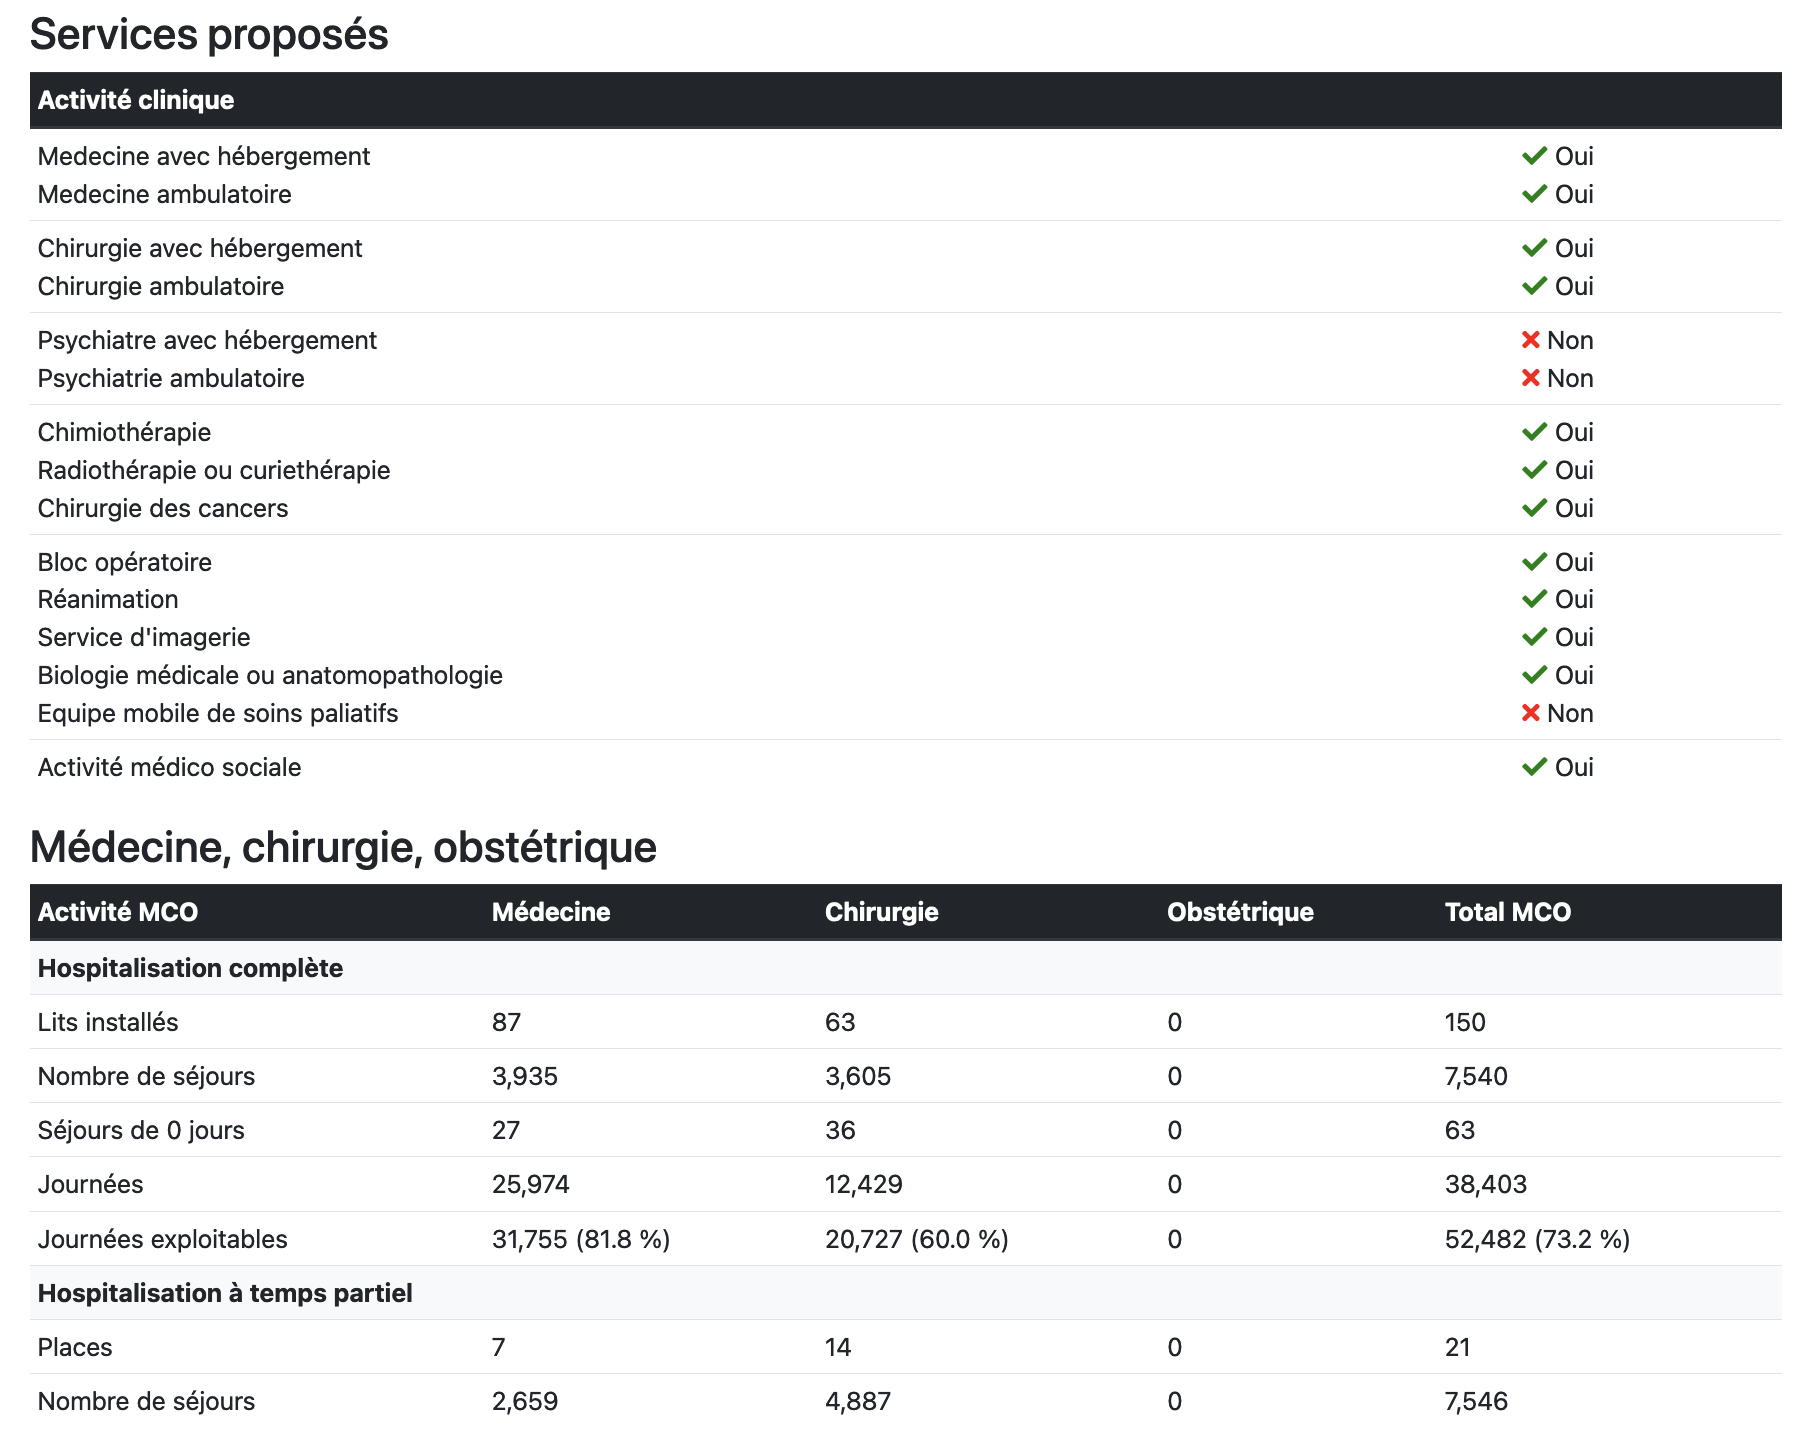
\includegraphics[width=0.7\textwidth]{images/healthcare-network/curie-services.png}
    \centering
    \caption{ \textbf{Healthcare-Network: description of health services
            offered, and statistics on \ac{mco} activity for Institut Curie Paris
            hospital.} The list of services allows to quickly evaluate the
        hospital ability to treat cancer patients. The number of stays and number of
        beds lets the users evaluate the hospital size, and how saturated it is.}
    \label{fig:hn-curie-services}
\end{figure}

Next, we display a section focused on oncology activity, we show statistics
related to cancer care, as illustrated on \cref{fig:hn-curie-cancero}. This
section lists the key oncology services like radiotherapy, cancer surgery and
chemotherapy authorization. The number of cancer related stays, the number of
radiotherapy stays as well as the number of beds dedicated to oncology are
shown.

\begin{figure}[h]
    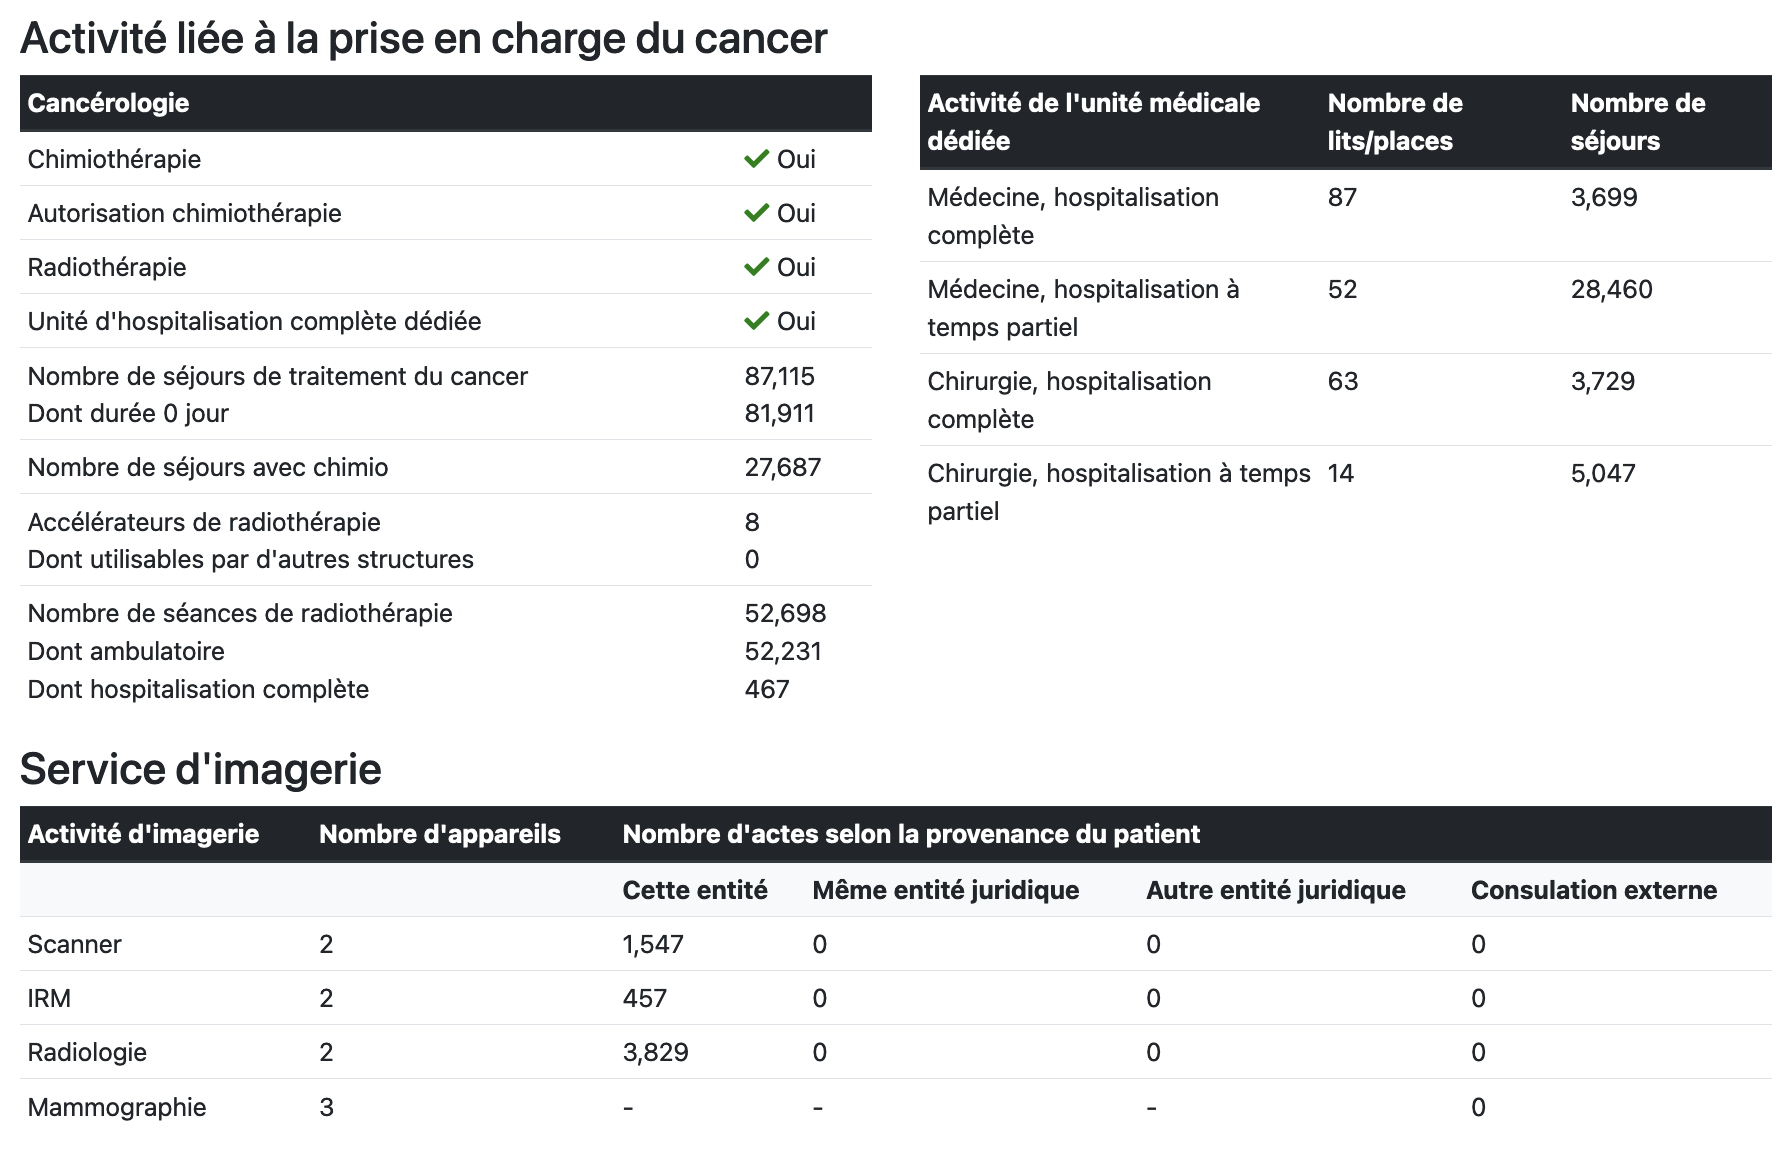
\includegraphics[width=0.7\textwidth]{images/healthcare-network/curie-cancero.png}
    \centering
    \caption{
        \textbf{Healthcare-Network: description of oncology activity for Institut Curie Paris hospital.}
    }
    \label{fig:hn-curie-cancero}
\end{figure}

Finally, we show the number of patients stays by cancer organs treated in the
hospital. We chose a radar chart visualization, as displayed on
\cref{fig:hn-curie-dp}. Three series are shown on this plot. First, in green, we
show the statistics of the current hospital. Then, in purple, we display the
median number of patients treated for every hospital in the same category, while
the orange curve shows the overall median. Showing these three variables allows
the users to compare the current hospital with hospitals within the same
category as well as broader comparison to the overall median. In this case, the
numbers are from Institut Curie hospital. The radar chart shows that this
hospital treats more patients than the other hospitals from the same category,
especially for eye cancer, where Institut Curie is among the only hospitals with
expertise on this rare cancer.

\begin{figure}[h]
    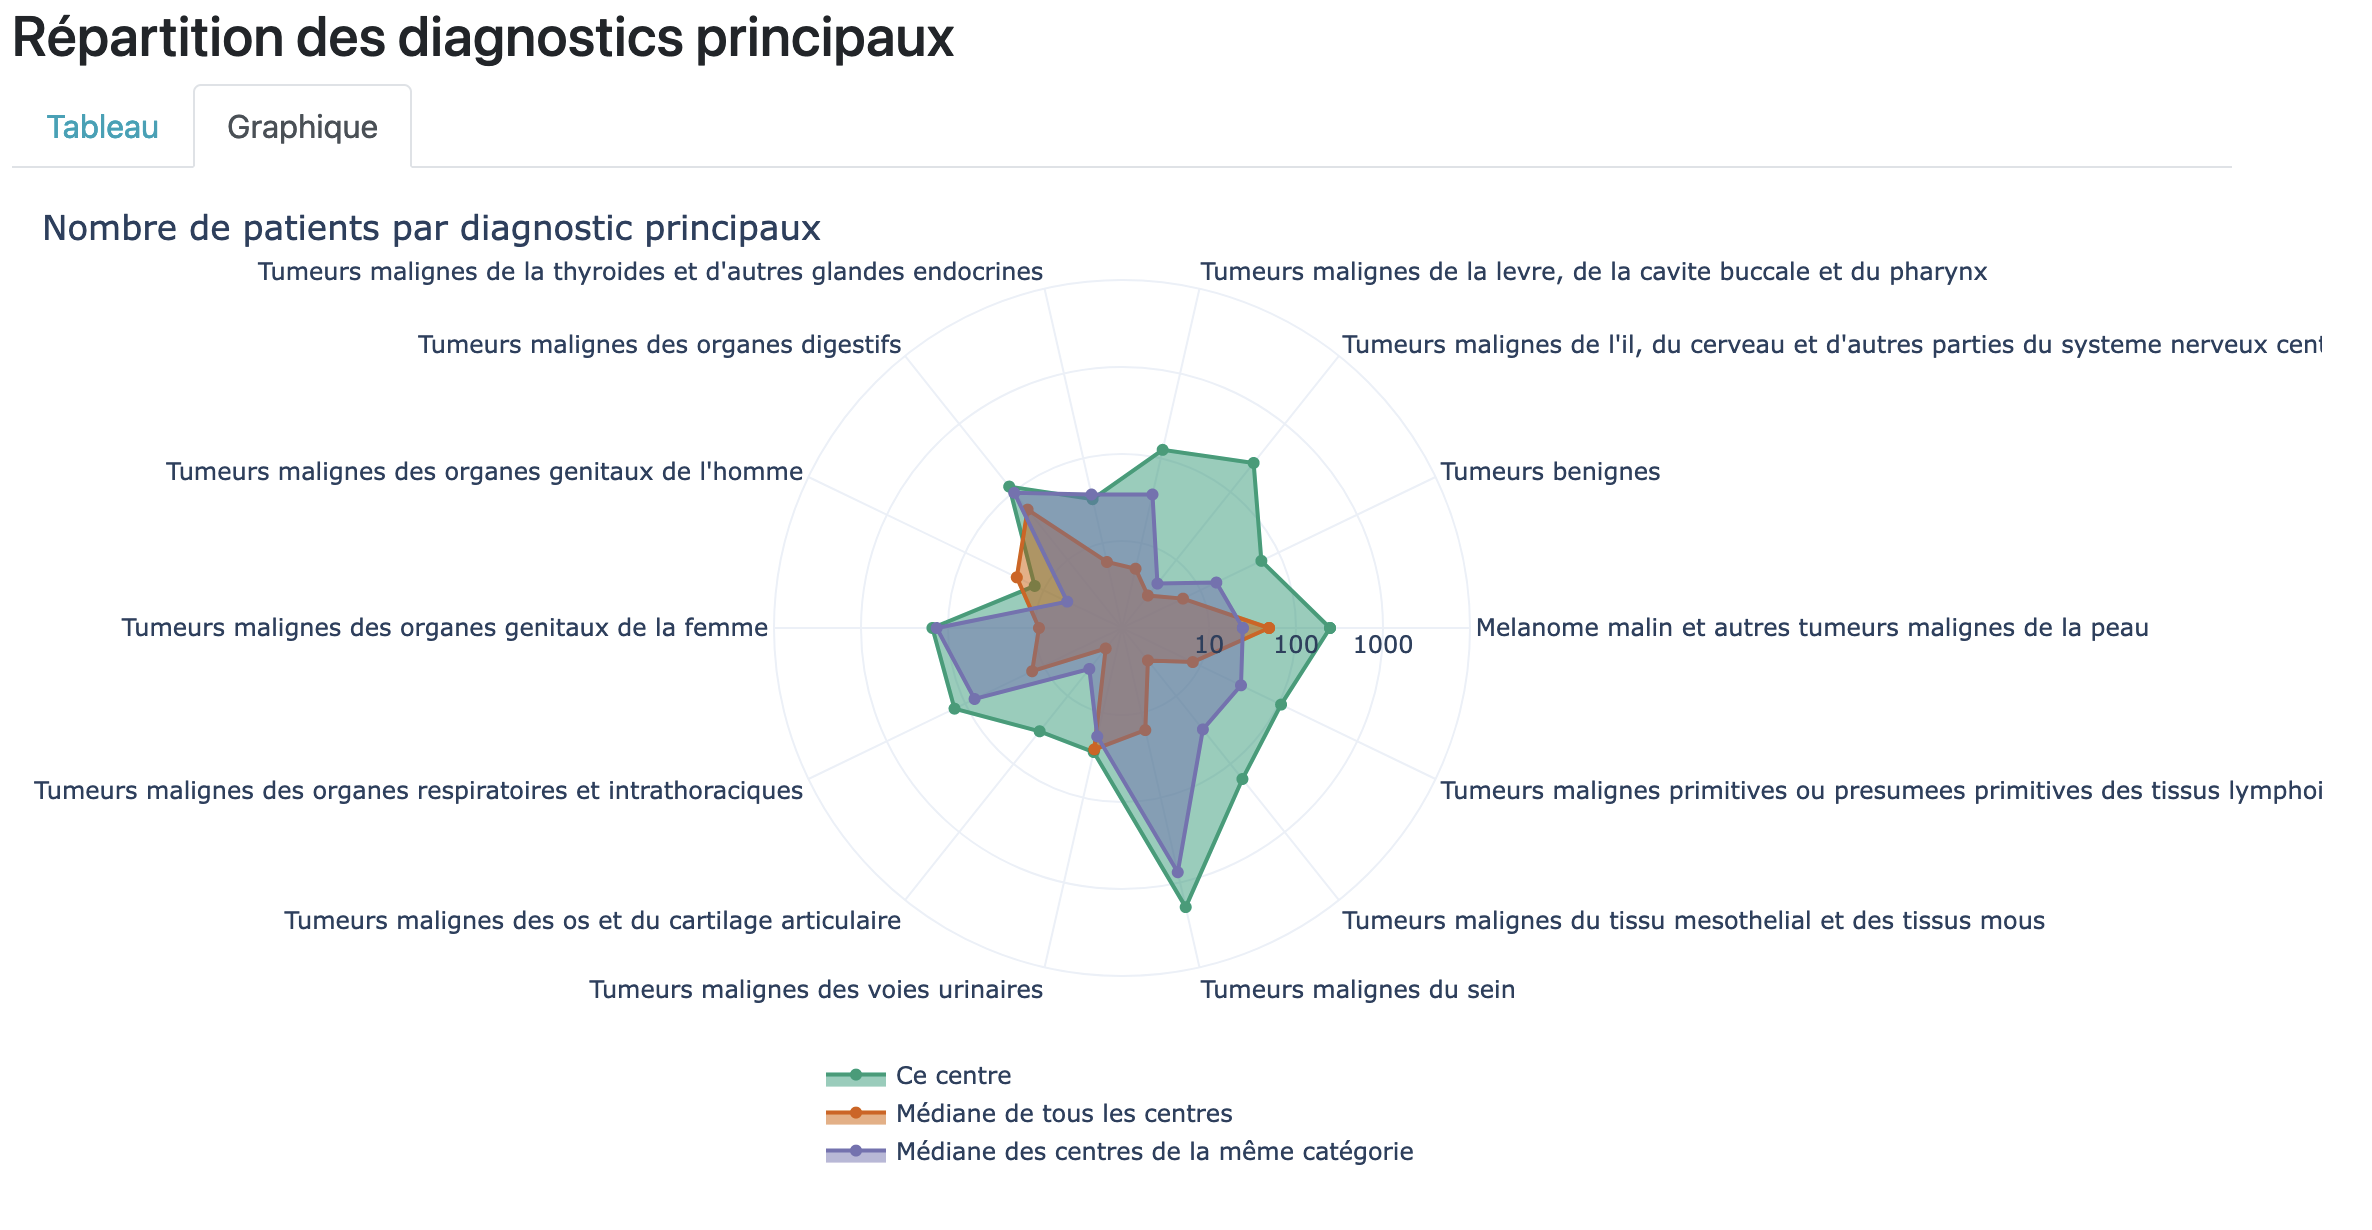
\includegraphics[width=0.7\textwidth]{images/healthcare-network/curie-dp.png}
    \centering
    \caption{ \textbf{Healthcare-Network: number of patients per cancer related
            diagnosis for Institut Curie Paris hospital.} Comparison with the median
        statistics from hospitals within the same category (\ac{clcc}) and
        overall median. }
    \label{fig:hn-curie-dp}
\end{figure}

To gain insights about the hospital neighborhood, we show socio-demographic
statistics on the municipality where the hospital is located. In the case of
Institut Curie, the municipality is the 5\textsuperscript{th} arrondissement of
Paris. Among the numbers displayed, we have the municipality size, population,
median salary and poverty rate. We also count the number of health professionals
by occupation within the hospital department, and within the hospital. This
gives information on the link between the hospital and the town medicine which
is very important for patient care.

\begin{figure}[h]
    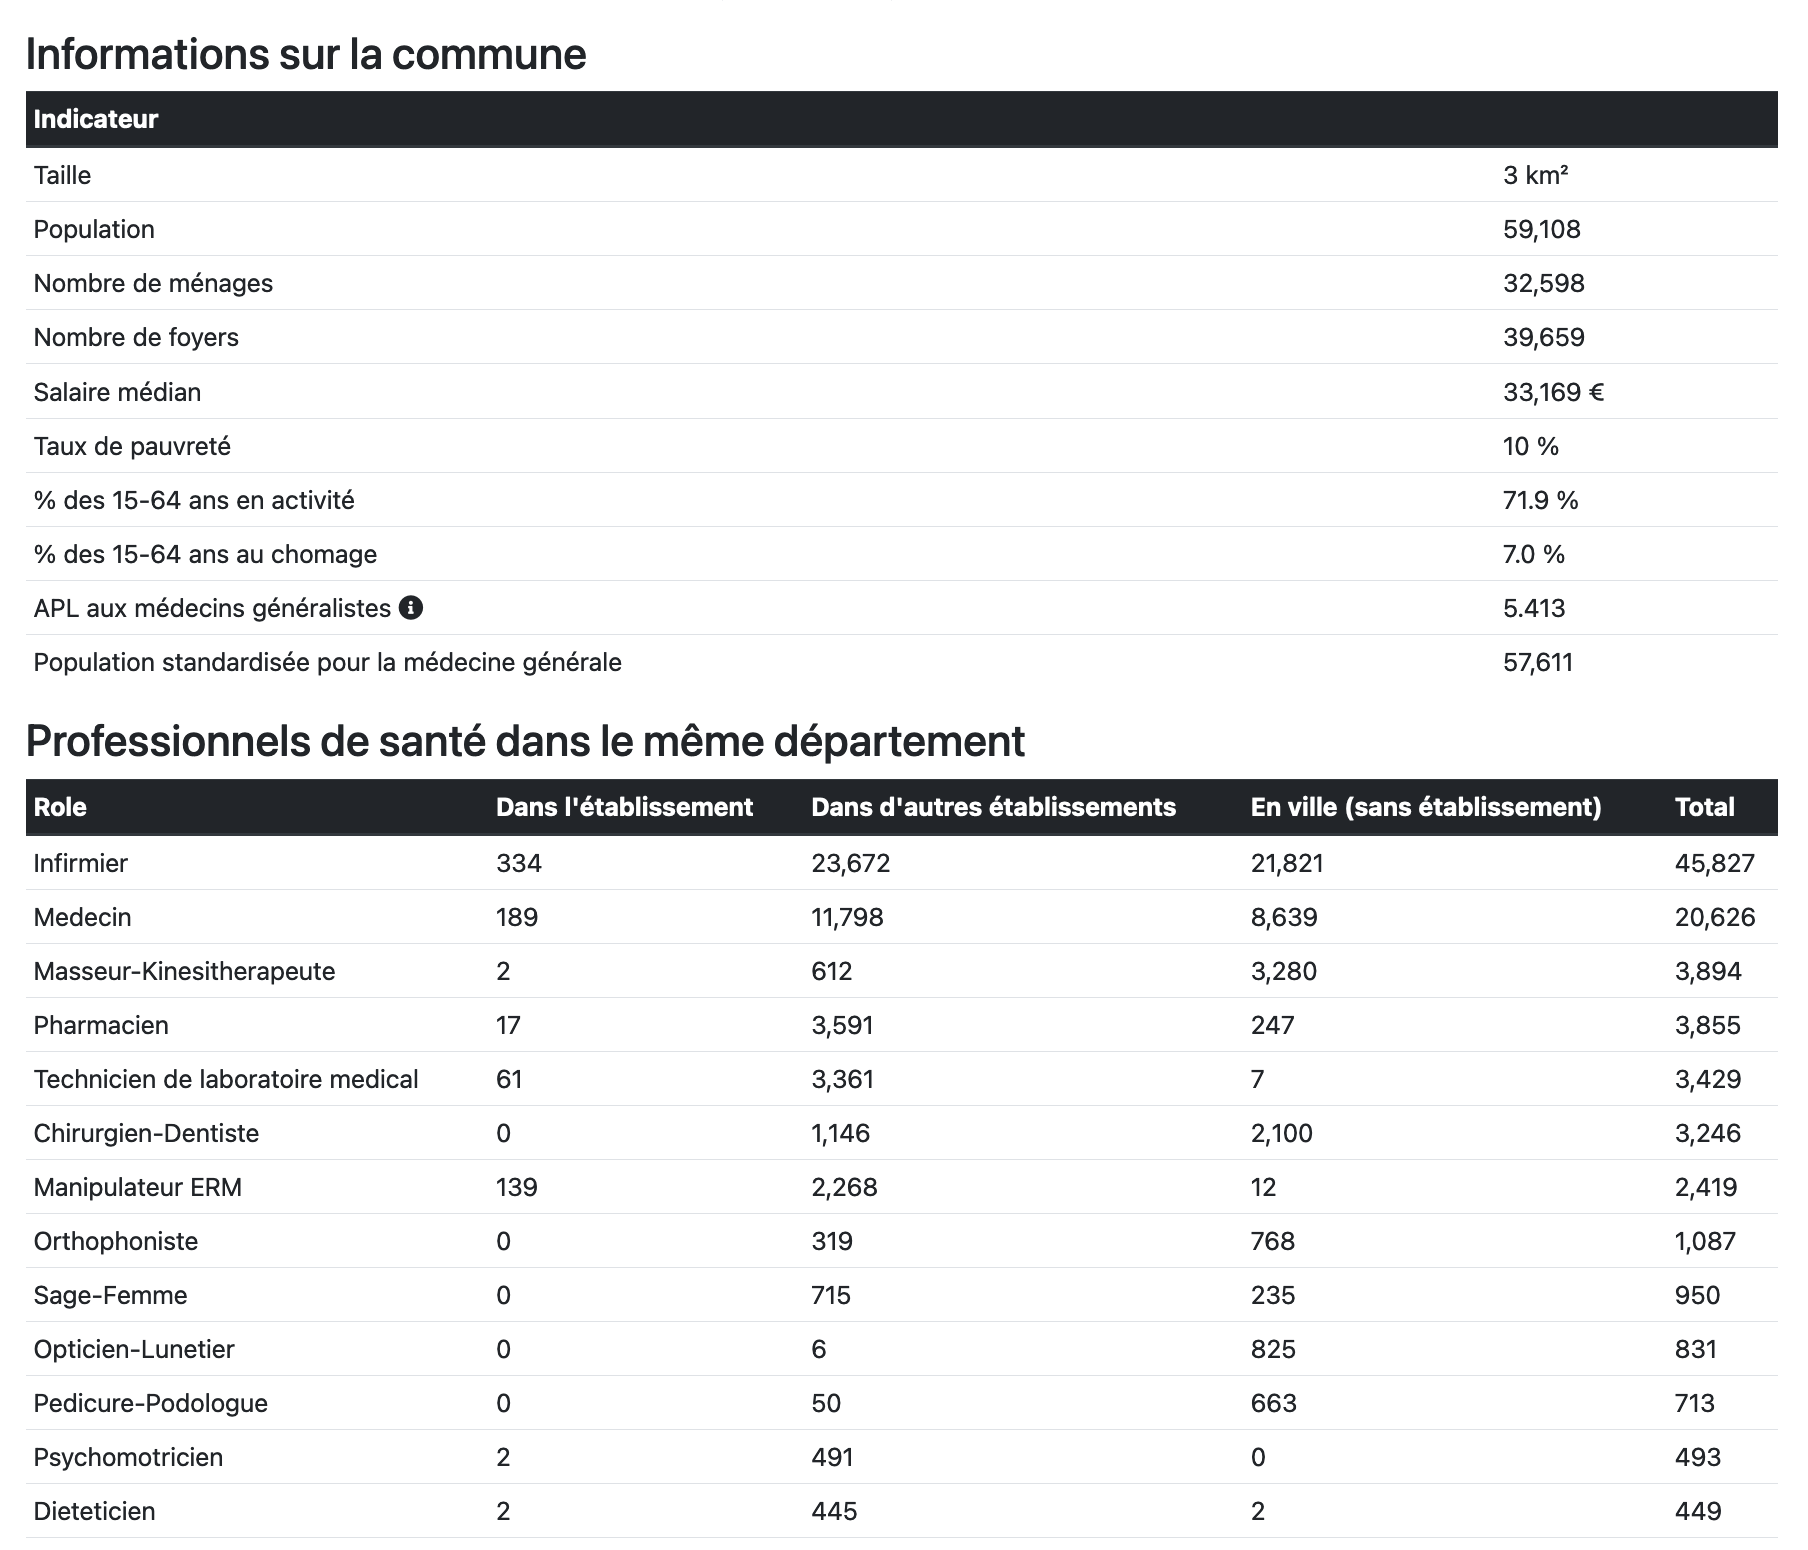
\includegraphics[width=0.7\textwidth]{images/healthcare-network/curie-commune.png}
    \centering
    \caption{ \textbf{Healthcare-Network: statistics on the municipality where
            Institut Curie Paris is located (Paris 75105).} Population, median
        salary and accessibility to primary care are displayed to qualify the
        hospital neighborhood. Health professionals within the department are
        also listed to illustrate the health supply available around the
        hospital. }
    \label{fig:hn-curie-commune}
\end{figure}

\section{Conclusion}

Our Healthcare-Network web application could benefit both patients and
healthcare professionals. It might incentive health professionals to find a
closer hospital from the patient location, lowering both travel burden as well
as \ac{co2} emissions. Also, patients will be able to double check where they
have been sent to, which could reduce dissatisfaction and health disparities. In
Healthcare-Network, hospitals statistics are displayed in the most transparent
way possible. This often involves showing plain numbers to patients or health
professionals, which might be confusing and unclear for some. More work might be
needed to make sure the web application is intuitive and brings useful
information to everyone. Moreover, while we developed the web application with
the help of medical experts, we did not gather patients' feedback yet. The app
design and features are thus likely to change in the future. While our web
application brings more health information to the patients, we should be
cautious about undesired effects of this approach. Indeed, research showed that
the increase in the amount of available medical information resulted in some
difficulties for patients when search-ing for suitable doctors
\cite{narducci_recommender_2015,hoens_reliable_2010}. This gap opened the need
for patient-doctor matchmaking, in which patients can find the right doctors
based on several criteria \cite{han_hybrid_2018}. Recommender systems are a
typical way to solve such problems. They have been integrated into online
retailers, streaming services, and social networks to facilitate users' item
selection process. Recently, these systems have been widely applied to the
healthcare domain to help both end-users and medical professionals in making
more efficient and accurate health related decisions
\cite{tran_recommender_2021}. Recommender systems have also been used to provide
personalized doctor recommendations based on emotions and preferences of users
about doctors through their ratings and reviews \cite{zhang_idoctor_2017}.
Although the current literature has shown many benefits of \ac{hrs} to improve
their health conditions, there still exist some gaps regarding developing and
evaluating \ac{hrs} that need to be bridged \cite{tran_recommender_2021},
especially during their evaluation \cite{calero_valdez_recommender_2016}.
Uncertainty in \ac{hrs} links to potential risks and imprecise predictions since
user preferences are not al-ways captured well. For these reasons, we chose not
to embed a hospital recommender system in the web application yet, since the
information we have on the patients are not detailed enough. Showing the health
facilities nearby the patients' location as well as some key statistics is a
good first step to assist patients and health professionals during the hospital
selection. Moreover, while mass media communications can be an important source
of health information, research found social disparities in health knowledge
that may be related to media use. Indeed, cancer-related health communications
seems to be patterned by race, ethnicity, language, and social class. The
benefits of health information are not equally distributed across socially
distinct groups in the United States \cite{viswanath_race_2011}. A lower
likelihood of cancer information seeking was also observed among those with
lower education levels, lower income and greater ages
\cite{finney_rutten_cancer-related_2016}. Therefore, we must make sure our tool
can be accessed by most of the patients, and efforts must be made in addressing
these social disparities. Improving healthcare by making it more connected will
not be sufficient as it will not benefit a non-insignificant part of the
population. The full benefits of a more connected and transparent healthcare
will show when the more deprived populations can access such tools.

  \chapter{\acf{simca}}

\section{Related work}
Hospital and practitioner recommendation has already been studied in the
literature (see e.g. the survey \cite{tran_recommender_2021}). However, to the
best of our knowledge, no existing method incorporates hospital capacity
constraints in the algorithm training. This tends to refer many users to the
same hospital, potentially saturating it and degrading the overall care quality.

Matrix factorization \cite{koren_matrix_2009} is among the most popular
collaborative filtering recommendation algorithms. Matrix factorization
characterizes every user $i$ and item $j$ by high-dimensional embeddings $u_i,
    v_j$, and predict the user-item affinity by the inner product $\langle u_i, v_j
    \rangle$. This method has already been applied for patient/doctor recommendation
\cite{zhang_idoctor_2017, han_hybrid_2018}. However, regular matrix
factorization is usually applied to simple recommendation problems, such as
movie recommendation: as already explained before, recommending locations brings
new challenges and requires a different approach \cite{zhao_survey_2016}.

Geographical influence has been integrated in the matrix factorization framework
to recommend locations or points of interest (POIs) \cite{li_rank-geofm_2015}:
moreover, the learning algorithm can be adapted by adding a capacity term in the
loss function \cite{christakopoulou_recommendation_2017}.

The Monge-Kantorovitch formulation of the classical \ac{ot} problem can be
rephrased as a linear program that can be computationally slow and unstable in
high dimension \cite{cuturi_sinkhorn_2013}: this problem is often approximated
by adding an entropy regularization term, and easily solved by Sinkhorn-Knopp's
algorithm \cite{cuturi_sinkhorn_2013}. Another important advantage of this
regularization is that the solution of the \ac{ot} problem becomes
differentiable with respect to the parameters, which explains why this step is
integrated in many learning algorithms
\cite{genevay_learning_2017,cuturi_soft-dtw_2018,tai_sinkhorn_2021}.

Most relevant for the present paper is the work from Dupuy, Galichon and Sun
\cite{dupuy_estimating_2016}. In this study, the authors address the inverse
optimal transport problem, that is, given vectors of characteristics $\bX \in
    \mathbb{R}^d$ and $\bY \in \mathbb{R}^{d'}$ and the joint distribution of the
optimal matching, the problem of recovering the affinity function of the form
$\phi(\bX,\bY)=\bX^T \bA \bY$, namely to estimate matrix $\bA$. The authors are
in the setting where they observe pairs of embeddings $(\bX_t,\bY_t)$ together
with the optimal \emph{regularized matching} $\pi^*$ -- that is the solution to
problem \eqref{eq:piSinkhorn} hereafter -- and build an estimator of $\bA$ with
low-rank constraints, the objective being to isolate important characteristics
that carry the most important weight in the matching procedure between $x$ and
$y$. We stress the fact that the setting is different in our study:
% first, the model is slightly more general, with an affinity matrix of the form
% $\bM_{i,j} = \phi(\bU_i,\bV_j,\bD_{i,j})$. Second, and more importantly,
we only observe in our case the embeddings $\bU$ of the users and a distance
matrix $\bD$, function $\phi$ is known as well as the \emph{pure matching}
$\sigma^*$ -- that is the solution of the linear assignment problem
\eqref{eq:sigmastarLAP} hereafter, which differs from $\pi^*$ -- and the aim is
to infer item embeddings $\bV$. In other words, we do not seek to reconstruct
the affinity matrix, but for the learning of items' positions in the user's
embeddings space, these positions acting as reference points, upon which
prediction of future allocations can be made. Another difference is that the
number of items is typically very small compared to the number of users, which
justifies that the items are considered static: we also incorporate
\emph{capacity constraints} on the allocation problem.

\section{Problem definition}

\subsection*{A model for latent and geographical affinity}

The setting of the problem is as follows. Consider $n$ \emph{users} $x_1,
    \ldots, x_n$ embedded in a latent space $\cX$ identified to $\mathbb{R}^d$, with
embeddings given by $\bU_1, \ldots, \bU_n$. Also consider $m$ \emph{items}
$y_1,\ldots, y_m$ embedded in $\cX$ with embeddings $\bV_1, \ldots, \bV_m$, with
$m \leq n$. To each user $x_i$ we assign a single item $y_j$, according to an
\emph{affinity matrix} $\bM \in \mathbb{R}^{n \times m}$ given by
\begin{equation*}\label{eq:def_M}
    \bM_{i,j} := \Phi(\bU_i,\bV_j,\bD_{i,j}),
\end{equation*} where $\bD \in \mathbb{R}^{n \times m}$ is known and may be thought of e.g. as a geographical distance matrix between users and items in the underlying euclidean space, say $\mathbb{R}^2$ (we stress the fact that this space is \emph{not} the embedding space $\cX$). We will denote $\bM = \Phi(\bU,\bV,\bD)$ in the sequel.

We also work under the following constraints: each item $y_j, j \in [m]$ can be
assigned to at most $\bC_j$ users. Where $\bC=(\bC_1,\ldots,\bC_m)$ is
\emph{capacity} vector. The \emph{total capacity} is defined by
\begin{equation*}
    s(\bC) := \sum_{j \in [m]} \bC_j,
\end{equation*} and we will assume $s(\bC) = n$.
We define
\begin{equation*}\label{eq:defSigma}
    \Sigma(n,m,\bC) := \left\lbrace \sigma \in \left\{ 0,1\right\}^{n \times m}, \; {\sigma \mathbf{1}_m}  = { \mathbf{1}_n}, {\sigma^T \mathbf{1}_n} = \bC \right\rbrace.
\end{equation*} In the sequel, $\sigma$ will denote both the assignment and its corresponding matrix representation. The optimal assignment $\sigma^*$ is given by
\begin{equation}\label{eq:sigmastarLAP}
    \sigma^*(\bU,\bV,\bD,\bC) := \argmax_{\sigma \in \Sigma(n,m,\bC)} \Tr\left( \sigma^T \bM \right),
\end{equation}
Note that problem \eqref{eq:sigmastarLAP} is an instance of the \emph{\ac{lap}}.

\subsection*{Goal} Assume that we are given the user embeddings $\bU$, the
distance matrix $\bD$, the capacities $\bC$ and the optimal assignment $\sigma^*
    \in \Sigma(n,m,\bC)$. The goal is to learn the item embeddings $\bV$.

\subsection*{Loss metrics, regularization and relaxation}
We will evaluate the performance of a proposed estimate $\widehat{\bV}$ of $\bV$
through the assignment $\widehat{\pi}$ obtained with $\widehat{\bV}$. To compare
$\widehat{\pi}$ with $\sigma^*$, we use the usual \emph{cross entropy loss}
defined by
\begin{equation*}
    H(\sigma^*,\widehat{\pi}) := - \sum_{i \in [n]} \log{\widehat{\pi}_{i,\sigma^*(i)}} = - \Tr\left( (\sigma^*)^T (\log \widehat{\pi}) \right).
\end{equation*}

% For simplicity, we will next focus on the case where the capacities satisfy
% $\sum_{j \in [m]} \bC_j = n$\todo{LG: je sais pas si on peut vraiment }. We
% will thus resize the matrix $\bM$ in order to have a square matrix: the
% indices $j$ now lie in $[n]$ and correspond to items $\left(y_1, \ldots, y_1,
% y_2, \ldots, y_{m-1}, y_m, \ldots y_m\right)$, where each item $j$ is repeated
% $\bC_j$ times. Problem \eqref{eq:sigmastar} then becomes

% \begin{equation}\label{eq:sigmastarLAP} \sigma^*(\bU,\bV,\bD,\bC) :=
%     \argmax_{\sigma \in \Sigma_n} \Tr\left( \sigma^T \bM \right),
%     \end{equation} where $\Sigma_n$ is the group of permutations of size $n$.

As stated before, from a learning perspective, a main issue is that the solution
to problem \eqref{eq:sigmastarLAP} is not differentiable w.r.t. $\bV$, the
variable of interest. This issue is solved by a relaxation/regularization
procedure \cite{cuturi_sinkhorn_2013}:
\begin{itemize}
    \item since the objective function is linear, we first consider the
          classical relaxation of \eqref{eq:sigmastarLAP} on the polytope of the
          convex hull of $\Sigma(n,m,\bC)$, namely on
          \begin{equation*}\label{eq:defPi}
              \Pi(n,m,\bC) := \left\lbrace \pi \in [0,1]^{n \times m}, \; {\pi \mathbf{1}_m}  = { \mathbf{1}_n}, {\pi^T \mathbf{1}_n} = \bC \right\rbrace.
          \end{equation*}
    \item moreover, we regularize the objective function in order to perform
          (automatic) differentiation: this is made possible by the classical entropy
          regularization in optimal transport.
\end{itemize}
For a small regularization parameter $\eps>0$, the problem then becomes
\begin{equation}\label{eq:piSinkhorn}
    \pi_{\eps}^*(\bU,\bV,\bD,\bC) := \argmax_{\pi \in \Pi(n,m,\bC)} \left[\Tr\left( \pi^T \bM \right) + \eps H(\pi) \right],
\end{equation} where
\begin{equation}\label{eq:Hpi}
    H(\pi) := - \sum_{1 \leq i,j \leq n} \pi_{i,j} (\log \pi_{i,j}-1).
\end{equation}

It is known in the literature \cite{cuturi_sinkhorn_2013} that the solution
$\pi_{\eps}^*$ to the convex optimization problem \eqref{eq:piSinkhorn} can be
easily computed with Sinkhorn-Knopp's algorithm, and has the following form:
\begin{equation}\label{eq:formesinkhorn}
    \left(\pi_{\eps}^* \right)_{i,j} = a_i \exp\left( \frac{1}{\eps} \bM_{i,j} \right) b_j,
\end{equation} where $a$ and $b$ are vectors of $\mathbb{R}_+^n$ and $\mathbb{R}_+^m$.
% The fact that $\pi^*_{\eps}(\bV)$ has an explicit, differentiable formulation
% in terms of $\bV$ justifies the use of such a regularized objective.
Note that we are back to our initial problem \eqref{eq:sigmastarLAP} when
$\eps=0$.

\subsection*{SiMCa Algorithm}
With this new formulation \eqref{eq:piSinkhorn}, we are now able to design an
optimization scheme for our learning problem. In our setting the users
embeddings $\bU$, the distance matrix $\bD$ and the capacities $\bC$ are known,
only the items embeddings $\bV$ are learned. The overall procedure is summarized
in Algorithm \ref{algo_learning_embeddings}. Given the current estimate $\bV_t$
at iteration $t$, we compute the solution $\pi^*_{\eps}(\bV_t)$ to problem
\eqref{eq:piSinkhorn}, which in turn is used to compute the gradient in $\bV_t$
of the following loss
\begin{equation}\label{eq:loss_global}
    \loss(\bV_t) := H\left(\sigma^*,\pi^*_{\eps}(\bV_t)\right)
\end{equation} to update our estimate of $\bV$ through a gradient step. The gradient in $\bV$
has actually a simple analytical expression:

\begin{lemma}\label{lemma:gradient} We have
    \begin{equation}
        \label{eq:gradient}
        \nabla_\bV \loss(\bV) = \frac{1}{\eps} \sum_{1 \leq i,j \leq n} (\pi^*_\eps(\bV) - \sigma^*)_{i,j} \nabla_\bV \bM_{i,j} \, .
    \end{equation}
\end{lemma}

\begin{proof}
    A very similar expression for the gradient is derived for the maximum likelihood
    in \cite{dupuy_estimating_2016}. We straightforwardly adapt their derivation to
    the cross entropy loss \eqref{eq:loss_global}. Let us denote
    \begin{equation}
        \label{eq:defV}
        V_\eps(\bM) = \max_{\pi \in \Pi(n,m,\bC)} \left[\Tr\left( \pi^T \bM \right) + \eps H(\pi) \right]
    \end{equation}
    the optimal value of the regularized \ac{ot} problem \eqref{eq:piSinkhorn}. As
    well-known in the \ac{ot} literature, see Proposition 9.2 of
    \cite{peyre_computational_2020}, its gradient with respect to the affinity
    matrix $M$ is given by the optimal coupling
    \begin{equation}
        \label{eq:gradV}
        \frac{\partial}{\partial \bM_{i, j}} V_\eps(\bM) =  (\pi^*_\eps)_{i, j}.
    \end{equation}
    Our cross-entropy loss \eqref{eq:loss_global} is directly related to the optimal
    value $V_\eps(\bM)$:
    \begin{flalign*}
        \loss = H\left(\sigma^*,\pi^*_{\eps}\right) & = - \sum_{i,j} \sigma^*_{i,j}
        \ln (\pi^*_\eps)_{i,j} \tag*{}                                                                                       \\
                                                    & \stackrel{1}{=} - \sum_{i,j} \sigma^*_{i,j} (\tfrac{1}{\eps}
        \bM_{i,j} + \ln a_i + \ln b_j)                                                                                       \\
                                                    & \stackrel{2}{=} -  \sum_{i,j} \sigma^*_{i,j} \tfrac{1}{\eps}
        \bM_{i,j}  - \sum_{i,j} (\pi^*_\eps)_{i,j} (\ln a_i + \ln b_j)                                                       \\
                                                    & \stackrel{3}{=} -  \sum_{i,j} \sigma^*_{i,j} \tfrac{1}{\eps}
        \bM_{i,j}  - \sum_{i,j} (\pi^*_\eps)_{i,j} (\ln (\pi^*_\eps)_{i,j} -
        \tfrac{1}{\eps} \bM_{i,j})                                                                                           \\
                                                    & \stackrel{4}{=} -  \sum_{i,j} \sigma^*_{i,j} \tfrac{1}{\eps}
        \bM_{i,j}  - s(\bC)                                                                                                  \\
                                                    & - \sum_{i,j} (\pi^*_\eps)_{i,j} (\ln (\pi^*_\eps)_{i,j} - 1) +
        \sum_{i,j} (\pi^*_\eps)_{i,j} \tfrac{1}{\eps} \bM_{i,j}                                                              \\
                                                    & \stackrel{5}{=} -s(\bC) + \tfrac{1}{\eps} [ \Tr(\pi^{*T}_\eps \bM) +
        \eps H(\pi^*_\eps) - \Tr(\sigma^{*T}\bM) ]                                                                           \\
                                                    & \stackrel{6}{=} -s(\bC) + \tfrac{1}{\eps} [ V_\eps(\bM) -
        \Tr(\sigma^{*T}\bM)].                       &                                                                      &
    \end{flalign*}

    The first and third equalities follow from \eqref{eq:formesinkhorn}, the second
    and fourth from $\sigma^*, \pi^*_\eps \in \Pi(n,m,\bC)$, the fifth from the
    definition \eqref{eq:Hpi} of $H(\pi)$ and the sixth from the definition
    \eqref{eq:defV} of $V_\eps(\bM)$. Then differentiating with respect to $\bV$
    leads to \eqref{eq:gradient} by the chain rule and \eqref{eq:gradV}.
\end{proof}

\begin{algorithm}[h]
    \caption{\ac{simca}}
    \label{algo_learning_embeddings}
    % \SetAlgoLined
    \begin{flushleft}
        \textbf{Input:} $\bU, \bD, \bC, \sigma^*$

        For $t =1$ to $T$:

        \begin{itemize}
            \item[$1.$] Compute the affinity matrix $\bM_{t-1} =
                    \Phi(\bU,\bV_{t-1},\bD)$.

            \item[$2.$]  Compute the solution to the optimization problem
                \eqref{eq:piSinkhorn}:
                \begin{equation*}
                    \pi_{\eps}^*(\bV_{t-1}) := \argmax_{\pi \in \Pi(n,m,\bC)} \left[\Tr\left( \pi^T \bM_{t-1} \right) + \eps H(\pi) \right].
                \end{equation*}

            \item[$3.$]  Compute the gradient $\nabla \loss(\bV_{t-1})$ with
                equation \eqref{eq:gradient}.

            \item[$4.$]  Perform a gradient step $\bV_{t} = \bV_{t-1} - \eta \nabla
                    \loss(\bV_{t-1})$.
        \end{itemize}
        \textbf{return} $\bV_T$
    \end{flushleft}
\end{algorithm}

The performance of our method is guaranteed by the following:
\begin{lemma}\label{lemma:convergence_guarantee} Assume that $v \mapsto
        \Phi(u,v,d)$ is linear. Then the loss function \eqref{eq:loss_global} is convex
    in $\bV$ and the output of \ac{simca} Algorithm (Algo.
    \ref{algo_learning_embeddings}) converges to
    \begin{equation*}
        \argmin_{\bV} H\left(\sigma^*,\pi^*_{\eps}(\bV)\right).
    \end{equation*}
\end{lemma}

\begin{proof}
    The proof of Lemma \ref{lemma:gradient} shows that
    \begin{equation*}
        \loss(V) = -s(\bC) + \tfrac{1}{\eps} [
            V_\eps(\bM) - \Tr(\sigma^{*T}\bM)].
    \end{equation*}
    Since $V \mapsto \Phi(\bU,V,\bD)$ is linear, $V \mapsto V_\eps(\bM)$, as defined
    in \eqref{eq:defV} is convex as a maximum of convex functions. By assumption, $V
        \mapsto \Tr(\sigma^{*T}\bM)$ is linear, thus $V \mapsto \loss(V)$ is convex.
\end{proof}

\section{Illustration for the hospital recommendation problem}
We now describe an illustration of our method for the hospital recommendation
problem. Since very few open datasets are available for this problem, we trained
our algorithm on synthetic data.

\subsection*{Dataset generation}
The dataset is generated as follows:
\begin{itemize}
    \item \textbf{Features in the embedding (latent) space:} we sample $n+m$
          points from a Gaussian mixture model with $k$ clusters. We set these points
          as either users ($\bU_i$) or items ($\bV_i$), and considered that each
          cluster must contain at least one item: we are thus left with $n$ users and
          $m$ items, spread between $k$ clusters. Users and items in the same cluster
          are considered similar. We then normalized both users and items features, so
          that all embeddings $\bU_i$ and $\bV_j$ lie on the unit sphere. Note that
          the users and items sampling is done independently of items capacities.

    \item \textbf{Distance in the underlying euclidean space:} to sample the
          distance matrix $\bD$ between users and items, we sample all the positions
          randomly on a circle, and computed the great-circle distance (i.e. spherical
          distance) between every users $i$ and items $j$. We finally normalize the
          distance matrix by its overall mean.

    \item \textbf{Capacities} we sampled $m$ values from a Dirichlet
          Distribution, corresponding to the probabilities that users are assigned to
          the $m$ items. We converted these probabilities into capacities $\bC_j$ by
          multiplying them with the number of users $n$. We then added some extra
          spots to each item.
\end{itemize}

\subsubsection*{Affinity matrix}
In our case, the affinity matrix $\bM=\Phi(\bU,\bV,\bD)$ is defined as follows:
\begin{equation}\label{eq:phi_def_illustration}
    \bM_{i,j}=\Phi(\bU_i,\bV_j,\bD_{i,j}) = (1-\alpha) \bU_i^T \bV_j - \alpha \bD_{i,j}.
\end{equation} The $\alpha$ coefficient measures the trade-off between affinity and proximity.

We then solve the Linear Assignment Problem \eqref{eq:sigmastarLAP} to compute
the pure matching $\sigma^*$.

\subsubsection*{Noise}
Noise is added to the original dataset in two different ways. The first method
is to modify the allocations of random users in $\sigma^*$, the noise ratio
being defined as the percentage of modified allocations\footnote{to make sure
    that the capacities constraints on the items still hold, we must swap
    \emph{pairs of users}: for a given allocation to modify, we pick another user
    randomly and swap their allocations.}. The second method consists in
perturbating $\bU$ as follows:
\begin{equation*}
    \widetilde{\bU} := \sqrt{1-\rho^2} \bU + \rho \bZ,
\end{equation*} where $\bZ$ is a matrix with i.i.d. standard Gaussian entries, and $\rho$ is the noise ratio.

\subsubsection*{Learning the embeddings}
Given $\bU$, $\bD$, $\bC$, $\sigma^*$, $\alpha$ and $\eps$, we compute an
estimate $\widehat{\bV}$ of the item embeddings with \ac{simca} Algorithm
(\cref{algo_learning_embeddings}). Comparing $\widehat{\bV}$ with $\bV$ gives a
first measure of the training performance.

\subsubsection*{Recovering the pure matching}
Then, using $\widetilde{\bU}$ (the noisy version of $\bU$), $\widehat{\bV}$ (the
estimated $\bV$), $\bD$, $\alpha$ and $\eps$, we compute the solution
$\widehat{\pi}^*_{\eps}$ to problem \eqref{eq:piSinkhorn}. Solving the \ac{lap}
on matrix $\widehat{\pi}^*_{\eps}$, we compute a pure matching
$\widehat{\sigma}^*$, which we can next compare to the original ${\sigma}^*$,
giving a second measure of the training performance.

\section{Results}

\subsubsection*{Parameters}
We generated a toy dataset with the following parameters: $n=1000$ users; $m=3$
items; $d=2$ latent features; $k=3$ clusters; $\alpha=0.3$. The items capacities
were 257, 417 and 356. \cref{fig:toy_dataset} shows the generated users and
items in both the embeddings (latent) space and their underlying euclidean
space.

\begin{figure}[h]
    \centering
    \includegraphics[width=.9\columnwidth]{images/simca/dataset.png}
    \caption{ \textbf{Generated dataset.} Users are displayed as crosses and
        items as circles, sized proportionally to their capacities. Users are
        colored accordingly to the item they have been allocated to. Plot (A)
        displays users and items in their shared embeddings (latent) space;
        where plot (B) displays them in their underlying euclidean space. }
    \label{fig:toy_dataset}
\end{figure}

\subsubsection*{Training results}
We trained our model with $\eps=0.1$ entropy regularization and $10$ iterations
in Sinkhorn-Knopp's algorithm to output $\widehat{\bV}$. As mentioned earlier we
compute a solution to the \ac{lap} on matrix $\widehat{\pi}^*_{\eps}$ to output
the estimated allocation $\widehat{\sigma}^*$. The model was trained with Adam
optimizer, with a $0.01$ learning rate and $400$ epochs. For the measures of
performance, we used the F1 score, for measuring how well the allocations are
reproduced, and the mean euclidean distance between learned embeddings
$\widehat{\bV}$ and the ground truth $\bV$. The training results are displayed
on \cref{fig:learned_embeddings}.

\begin{figure}[h]
    \centering
    \includegraphics[width=.9\columnwidth]{images/simca/learned_embeddings.png}
    \caption{ \textbf{Training results.} We can see that the model achieves good
        performances to learn the item embeddings (A), and recovers the
        allocation with a close to 1 F1 score (B). The average distance between
        the learned embeddings and ground truth decreases during training (C). }
    \label{fig:learned_embeddings}
\end{figure}

\subsubsection*{Influence of entropy regularization}
We investigate the influence of the entropy regularization parameter $\eps$ on
the model performance. We let $\eps$ vary between $0.05$ and $2$, with the same
dataset and the same model parameters\footnote{due to numerical instability, the
    algorithm could not train properly above $\eps = 0.05$.}. We ran 5 training for
every value of $\eps$. As shown on \cref{fig:experiment_epsilon}, the training
performance worsens when $\eps$ increases.

\begin{figure}[h]
    \centering
    \includegraphics[width=.45\columnwidth]{images/simca/experiment_epsilon_boxplot.png}
    \caption{ \textbf{Performance as a function of $\eps$.} Increasing $\eps$
        leads to lower F1 scores. }
    \label{fig:experiment_epsilon}
\end{figure}

\subsubsection*{Influence of noise}
We study the influence of noise, either by swapping allocations or adding
Gaussian noise to the used embeddings, as described in the previous section.
Unsurprisingly, as shown in \cref{fig:experiment_noise}, the training
performance is decreasing with the noise ratio.

\begin{figure}[h]
    \centering
    \includegraphics[width=.9\columnwidth]{images/simca/experiment_noise_boxplot.png}
    \caption{ \textbf{Influence of adding Gaussian noise (A) and swapping
            allocations (B) on training performance.} F1 score decreases as noise
        increases. }
    \label{fig:experiment_noise}
\end{figure}

\subsubsection*{Learning both users and items embeddings}

We also studied the case where the users' embeddings are not known, and must be
learned jointly with the items' embeddings from the observed allocations. In
this case, we initialized the items' and users' embeddings similarly. We managed
to retrieve the observed allocation as illustrated on
\cref{fig:experiment_learn_users_embeddings}. However, the average distance
between learned items embeddings and ground truth does not decrease during
training, meaning that the model learned its own interpretation of the users'
and items' representations to satisfy the observed mapping.

\begin{figure}[h]
    \centering
    \includegraphics[width=.9\columnwidth]{images/simca/experiment_learn_both_embeddings.png}
    \caption{ \textbf{Learning both users and items embeddings simultaneously.}
        The learned embeddings are shown on (A). The model retrieves the
        observed allocation (B). However, the average distance between learned
        items embeddings and ground truth does not decrease during training (C).
    }
    \label{fig:experiment_learn_users_embeddings}
\end{figure}

  \chapter*{Conclusion}
\addcontentsline{toc}{chapter}{Conclusion}


\end{singlespace}

%**********************
%***** References *****
%**********************

\newgeometry{top=4cm, bottom=4cm, left=2cm, right=2cm}

\bibliographystyle{vancouver}
\bibliography{references}

%**************************************
%***** List of tables and figures *****
%**************************************

\newgeometry{top=4cm, bottom=4cm, left=2cm, right=2cm}

\listoffigures
\listoftables

%********************
% 4eme de couverture
%********************

\checkoddpage
\ifoddpage \newpage\thispagestyle{empty}\null\newpage \fi

\thispagestyle{empty}
\newgeometry{top=1.5cm, bottom=1.25cm, left=2cm, right=2cm}
\fontfamily{rm}\selectfont

\lhead{}
\rhead{}
\rfoot{}
\cfoot{}
\lfoot{}

\noindent

\includegraphics[height=2.45cm]{images/logos/logo_usp_CBMS.png}
\vspace{1cm}

\fontfamily{cmss}\fontseries{m}\selectfont

\small

\begin{mdframed}[linecolor=Prune,linewidth=1]

    \textbf{Titre:} Etude des disparités géographiques et socio-démographiques dans les parcours de soins en oncologie.

    \noindent \textbf{Mots clés:} 3 à 6 mots clefs (version en français)

    \vspace{-.5cm}
    \begin{multicols}{2}
        \noindent \textbf{Résumé:} On estime à 382 000 le nombre de nouveaux cas de
        cancers incidents et à 157 400 le nombre de décès en 2018 en France. Le Plan
        Cancer 2014-2019 annonce les objectifs à mettre en oeuvre dans la lutte contre le
        cancer en France. En particulier, les objectifs 2 et 7 insistent sur la qualité
        du parcours de soin : ils ambitionnent respectivement de ``garantir la qualité
        et la sécurité des prises en charge'' et ``assurer des prises en charge globales
        et personnalisés''. Dans le but de standardiser le parcours de soin tout en
        personnalisant la prise en charge, des trajectoires de soin ont été instaurées.
        La définition de ces trajectoires de soin optimales s'appuie sur des
        recommandations de bonnes pratiques nationales et internationales. Nous
        proposons d'étudier en détails les disparités géographiques et
        socio-démographiques dans les parcours de soin des patients atteints d'un cancer
        en France. Dans un premier temps, nous chercherons à caractériser les
        établissements de santé en France à partir de leur activité en oncologie. Puis,
        nous étudierons la distribution de ces centres sur le territoire, afin de mettre
        en évidence d'éventuelles disparités dans l'accès à ceux-ci. Enfin, nous
        tenterons de proposer un algorithme de recommandations de centres de soins, à
        partir des données du Système National des Données de Santé (SNDS). Cet
        algorithme aura pour but de guider les patients vers le centre optimal, en vue
        de maximiser la qualité du parcours de soins.

    \end{multicols}

\end{mdframed}


\vspace{8mm}

\begin{mdframed}[linecolor=Prune,linewidth=1]

\textbf{Title:} Geographic and socio-demographic disparities in oncology care pathways.

\noindent \textbf{Keywords:} 3 à 6 mots clefs (version en anglais)

\vspace{-.5cm}
\begin{multicols}{2}
\noindent \textbf{Abstract:} In France, during year 2018, there was 382,000 new cancer cases and 157,400 deaths. The 2014-2019 Cancer Plan sets new objectives for cancer care in France. In particular, objectives 2 and 7 emphasize the quality of the care pathways: they aim respectively to guarantee the quality and safety of care and ensure comprehensive and personalized care. In order to standardize the care pathways while personalizing care, care trajectories have been introduced. The definition of these optimal care trajectories is based on national and international good practice recommendations. We propose to study in detail the geographical and socio-demographic disparities in the care pathways of cancer patients in France. First, we will try to characterize the health care institutions in France based on their oncology activity. Then, we will study the distribution of these centers on the territory, in order to highlight possible disparities in access to them. Finally, we will try to propose a care center recommendation algorithm, using the French social security database (SNDS). This algorithm will aim at guiding patients towards the optimal center, in order to maximize the quality of the care pathways.

\end{multicols}
\end{mdframed}

%%%%%%%%%%%%%%%%%%%%%%%%%%
% Section headers format %
%%%%%%%%%%%%%%%%%%%%%%%%%%

\titleformat{\chapter}[hang]{\bfseries\Large\color{Prune}}{\thechapter\ -}{.1ex}
{\vspace{0.1ex}
}
[\vspace{1ex}]
\titlespacing{\chapter}{0pc}{0ex}{0.5pc}

\titleformat{\section}[hang]{\bfseries\normalsize}{\thesection\ .}{0.5pt}
{\vspace{0.1ex}
}
[\vspace{0.1ex}]
\titlespacing{\section}{1.5pc}{4ex plus .1ex minus .2ex}{.8pc}

\titleformat{\subsection}[hang]{\bfseries\small}{\thesubsection\ .}{1pt}
{\vspace{0.1ex}
}
[\vspace{0.1ex}]
\titlespacing{\subsection}{3pc}{2ex plus .1ex minus .2ex}{.1pc}

\end{document}
